\documentclass[]{book}
\usepackage{lmodern}
\usepackage{amssymb,amsmath}
\usepackage{ifxetex,ifluatex}
\usepackage{fixltx2e} % provides \textsubscript
\ifnum 0\ifxetex 1\fi\ifluatex 1\fi=0 % if pdftex
  \usepackage[T1]{fontenc}
  \usepackage[utf8]{inputenc}
\else % if luatex or xelatex
  \ifxetex
    \usepackage{mathspec}
  \else
    \usepackage{fontspec}
  \fi
  \defaultfontfeatures{Ligatures=TeX,Scale=MatchLowercase}
\fi
% use upquote if available, for straight quotes in verbatim environments
\IfFileExists{upquote.sty}{\usepackage{upquote}}{}
% use microtype if available
\IfFileExists{microtype.sty}{%
\usepackage{microtype}
\UseMicrotypeSet[protrusion]{basicmath} % disable protrusion for tt fonts
}{}
\usepackage{hyperref}
\hypersetup{unicode=true,
            pdftitle={Розеттский камень},
            pdfauthor={Пуассон, фея и три мексиканских негодяя},
            pdfborder={0 0 0},
            breaklinks=true}
\urlstyle{same}  % don't use monospace font for urls
\usepackage{natbib}
\bibliographystyle{apalike}
\usepackage{color}
\usepackage{fancyvrb}
\newcommand{\VerbBar}{|}
\newcommand{\VERB}{\Verb[commandchars=\\\{\}]}
\DefineVerbatimEnvironment{Highlighting}{Verbatim}{commandchars=\\\{\}}
% Add ',fontsize=\small' for more characters per line
\usepackage{framed}
\definecolor{shadecolor}{RGB}{248,248,248}
\newenvironment{Shaded}{\begin{snugshade}}{\end{snugshade}}
\newcommand{\AlertTok}[1]{\textcolor[rgb]{0.94,0.16,0.16}{#1}}
\newcommand{\AnnotationTok}[1]{\textcolor[rgb]{0.56,0.35,0.01}{\textbf{\textit{#1}}}}
\newcommand{\AttributeTok}[1]{\textcolor[rgb]{0.77,0.63,0.00}{#1}}
\newcommand{\BaseNTok}[1]{\textcolor[rgb]{0.00,0.00,0.81}{#1}}
\newcommand{\BuiltInTok}[1]{#1}
\newcommand{\CharTok}[1]{\textcolor[rgb]{0.31,0.60,0.02}{#1}}
\newcommand{\CommentTok}[1]{\textcolor[rgb]{0.56,0.35,0.01}{\textit{#1}}}
\newcommand{\CommentVarTok}[1]{\textcolor[rgb]{0.56,0.35,0.01}{\textbf{\textit{#1}}}}
\newcommand{\ConstantTok}[1]{\textcolor[rgb]{0.00,0.00,0.00}{#1}}
\newcommand{\ControlFlowTok}[1]{\textcolor[rgb]{0.13,0.29,0.53}{\textbf{#1}}}
\newcommand{\DataTypeTok}[1]{\textcolor[rgb]{0.13,0.29,0.53}{#1}}
\newcommand{\DecValTok}[1]{\textcolor[rgb]{0.00,0.00,0.81}{#1}}
\newcommand{\DocumentationTok}[1]{\textcolor[rgb]{0.56,0.35,0.01}{\textbf{\textit{#1}}}}
\newcommand{\ErrorTok}[1]{\textcolor[rgb]{0.64,0.00,0.00}{\textbf{#1}}}
\newcommand{\ExtensionTok}[1]{#1}
\newcommand{\FloatTok}[1]{\textcolor[rgb]{0.00,0.00,0.81}{#1}}
\newcommand{\FunctionTok}[1]{\textcolor[rgb]{0.00,0.00,0.00}{#1}}
\newcommand{\ImportTok}[1]{#1}
\newcommand{\InformationTok}[1]{\textcolor[rgb]{0.56,0.35,0.01}{\textbf{\textit{#1}}}}
\newcommand{\KeywordTok}[1]{\textcolor[rgb]{0.13,0.29,0.53}{\textbf{#1}}}
\newcommand{\NormalTok}[1]{#1}
\newcommand{\OperatorTok}[1]{\textcolor[rgb]{0.81,0.36,0.00}{\textbf{#1}}}
\newcommand{\OtherTok}[1]{\textcolor[rgb]{0.56,0.35,0.01}{#1}}
\newcommand{\PreprocessorTok}[1]{\textcolor[rgb]{0.56,0.35,0.01}{\textit{#1}}}
\newcommand{\RegionMarkerTok}[1]{#1}
\newcommand{\SpecialCharTok}[1]{\textcolor[rgb]{0.00,0.00,0.00}{#1}}
\newcommand{\SpecialStringTok}[1]{\textcolor[rgb]{0.31,0.60,0.02}{#1}}
\newcommand{\StringTok}[1]{\textcolor[rgb]{0.31,0.60,0.02}{#1}}
\newcommand{\VariableTok}[1]{\textcolor[rgb]{0.00,0.00,0.00}{#1}}
\newcommand{\VerbatimStringTok}[1]{\textcolor[rgb]{0.31,0.60,0.02}{#1}}
\newcommand{\WarningTok}[1]{\textcolor[rgb]{0.56,0.35,0.01}{\textbf{\textit{#1}}}}
\usepackage{longtable,booktabs}
\usepackage{graphicx,grffile}
\makeatletter
\def\maxwidth{\ifdim\Gin@nat@width>\linewidth\linewidth\else\Gin@nat@width\fi}
\def\maxheight{\ifdim\Gin@nat@height>\textheight\textheight\else\Gin@nat@height\fi}
\makeatother
% Scale images if necessary, so that they will not overflow the page
% margins by default, and it is still possible to overwrite the defaults
% using explicit options in \includegraphics[width, height, ...]{}
\setkeys{Gin}{width=\maxwidth,height=\maxheight,keepaspectratio}
\IfFileExists{parskip.sty}{%
\usepackage{parskip}
}{% else
\setlength{\parindent}{0pt}
\setlength{\parskip}{6pt plus 2pt minus 1pt}
}
\setlength{\emergencystretch}{3em}  % prevent overfull lines
\providecommand{\tightlist}{%
  \setlength{\itemsep}{0pt}\setlength{\parskip}{0pt}}
\setcounter{secnumdepth}{5}
% Redefines (sub)paragraphs to behave more like sections
\ifx\paragraph\undefined\else
\let\oldparagraph\paragraph
\renewcommand{\paragraph}[1]{\oldparagraph{#1}\mbox{}}
\fi
\ifx\subparagraph\undefined\else
\let\oldsubparagraph\subparagraph
\renewcommand{\subparagraph}[1]{\oldsubparagraph{#1}\mbox{}}
\fi

%%% Use protect on footnotes to avoid problems with footnotes in titles
\let\rmarkdownfootnote\footnote%
\def\footnote{\protect\rmarkdownfootnote}

%%% Change title format to be more compact
\usepackage{titling}

% Create subtitle command for use in maketitle
\providecommand{\subtitle}[1]{
  \posttitle{
    \begin{center}\large#1\end{center}
    }
}

\setlength{\droptitle}{-2em}

  \title{Розеттский камень}
    \pretitle{\vspace{\droptitle}\centering\huge}
  \posttitle{\par}
    \author{Пуассон, фея и три мексиканских негодяя}
    \preauthor{\centering\large\emph}
  \postauthor{\par}
      \predate{\centering\large\emph}
  \postdate{\par}
    \date{2019-09-23}

\usepackage{booktabs} % красивые таблицы
\usepackage{polyglossia} % переключение языков в xelatex
\setmainlanguage{russian} 
\newfontfamily{\cyrillicfont}{Linux Libertine O} % залатываем какой-то косяк с русскими шрифтами
\newfontfamily{\cyrillicfonttt}{Linux Libertine O}

\begin{document}
\maketitle

{
\setcounter{tocdepth}{1}
\tableofcontents
}
\hypertarget{-}{%
\chapter{Напутственное слово}\label{-}}

\hypertarget{installsoft}{%
\chapter{Коан об установке софта}\label{installsoft}}

В этом коане мы рассмотрим установку и настройку программ для работы на языках программирования R и Python, а также установку и настройку программы Stata.

\begin{center}\rule{0.5\linewidth}{\linethickness}\end{center}

\#\#\#Язык программирования R
\textgreater{} R - это открытая среда программирования, помогающая в работе со статистическими данными. Для программирования на R подойдет программа RStudio.

Рассмотрим установку RStudio на Mac OS и Windows.

\#\#\#\#\#Инструкция по установке RStudio для Windows / Mac OS:

\begin{enumerate}
\def\labelenumi{\arabic{enumi}.}
\tightlist
\item
  Загрузите и установите язык программирования R \href{http://cran.cnr.berkeley.edu/}{с официального сайта}.
\end{enumerate}

\begin{itemize}
\item
  Версия для Windows: Выберите ``Download R for Windows'' ▶ ``base'' ▶ ``Download R 3.x.x for Windows''.
\item
  Версия для Mac OS: Выберите ``Download R for (Mac) OS X'' ▶ ``Latest Release'' ▶ ``R 3.x.x''.
\end{itemize}

\begin{enumerate}
\def\labelenumi{\arabic{enumi}.}
\setcounter{enumi}{1}
\tightlist
\item
  Загрузите программу RStudio \href{https://www.rstudio.com/products/rstudio/download/}{с официального сайта разработчика} (выберите подходящую версию из предложенных опций). Возможностей бесплатной версии
  будет вполне достаточно для работы.
  
\includegraphics{images/RStudio.png}
\end{enumerate}

Готово, Вы можете использовать RStudio на вашем компьютере.

\#\#\#\#\#Начало работы

\begin{figure}
\centering
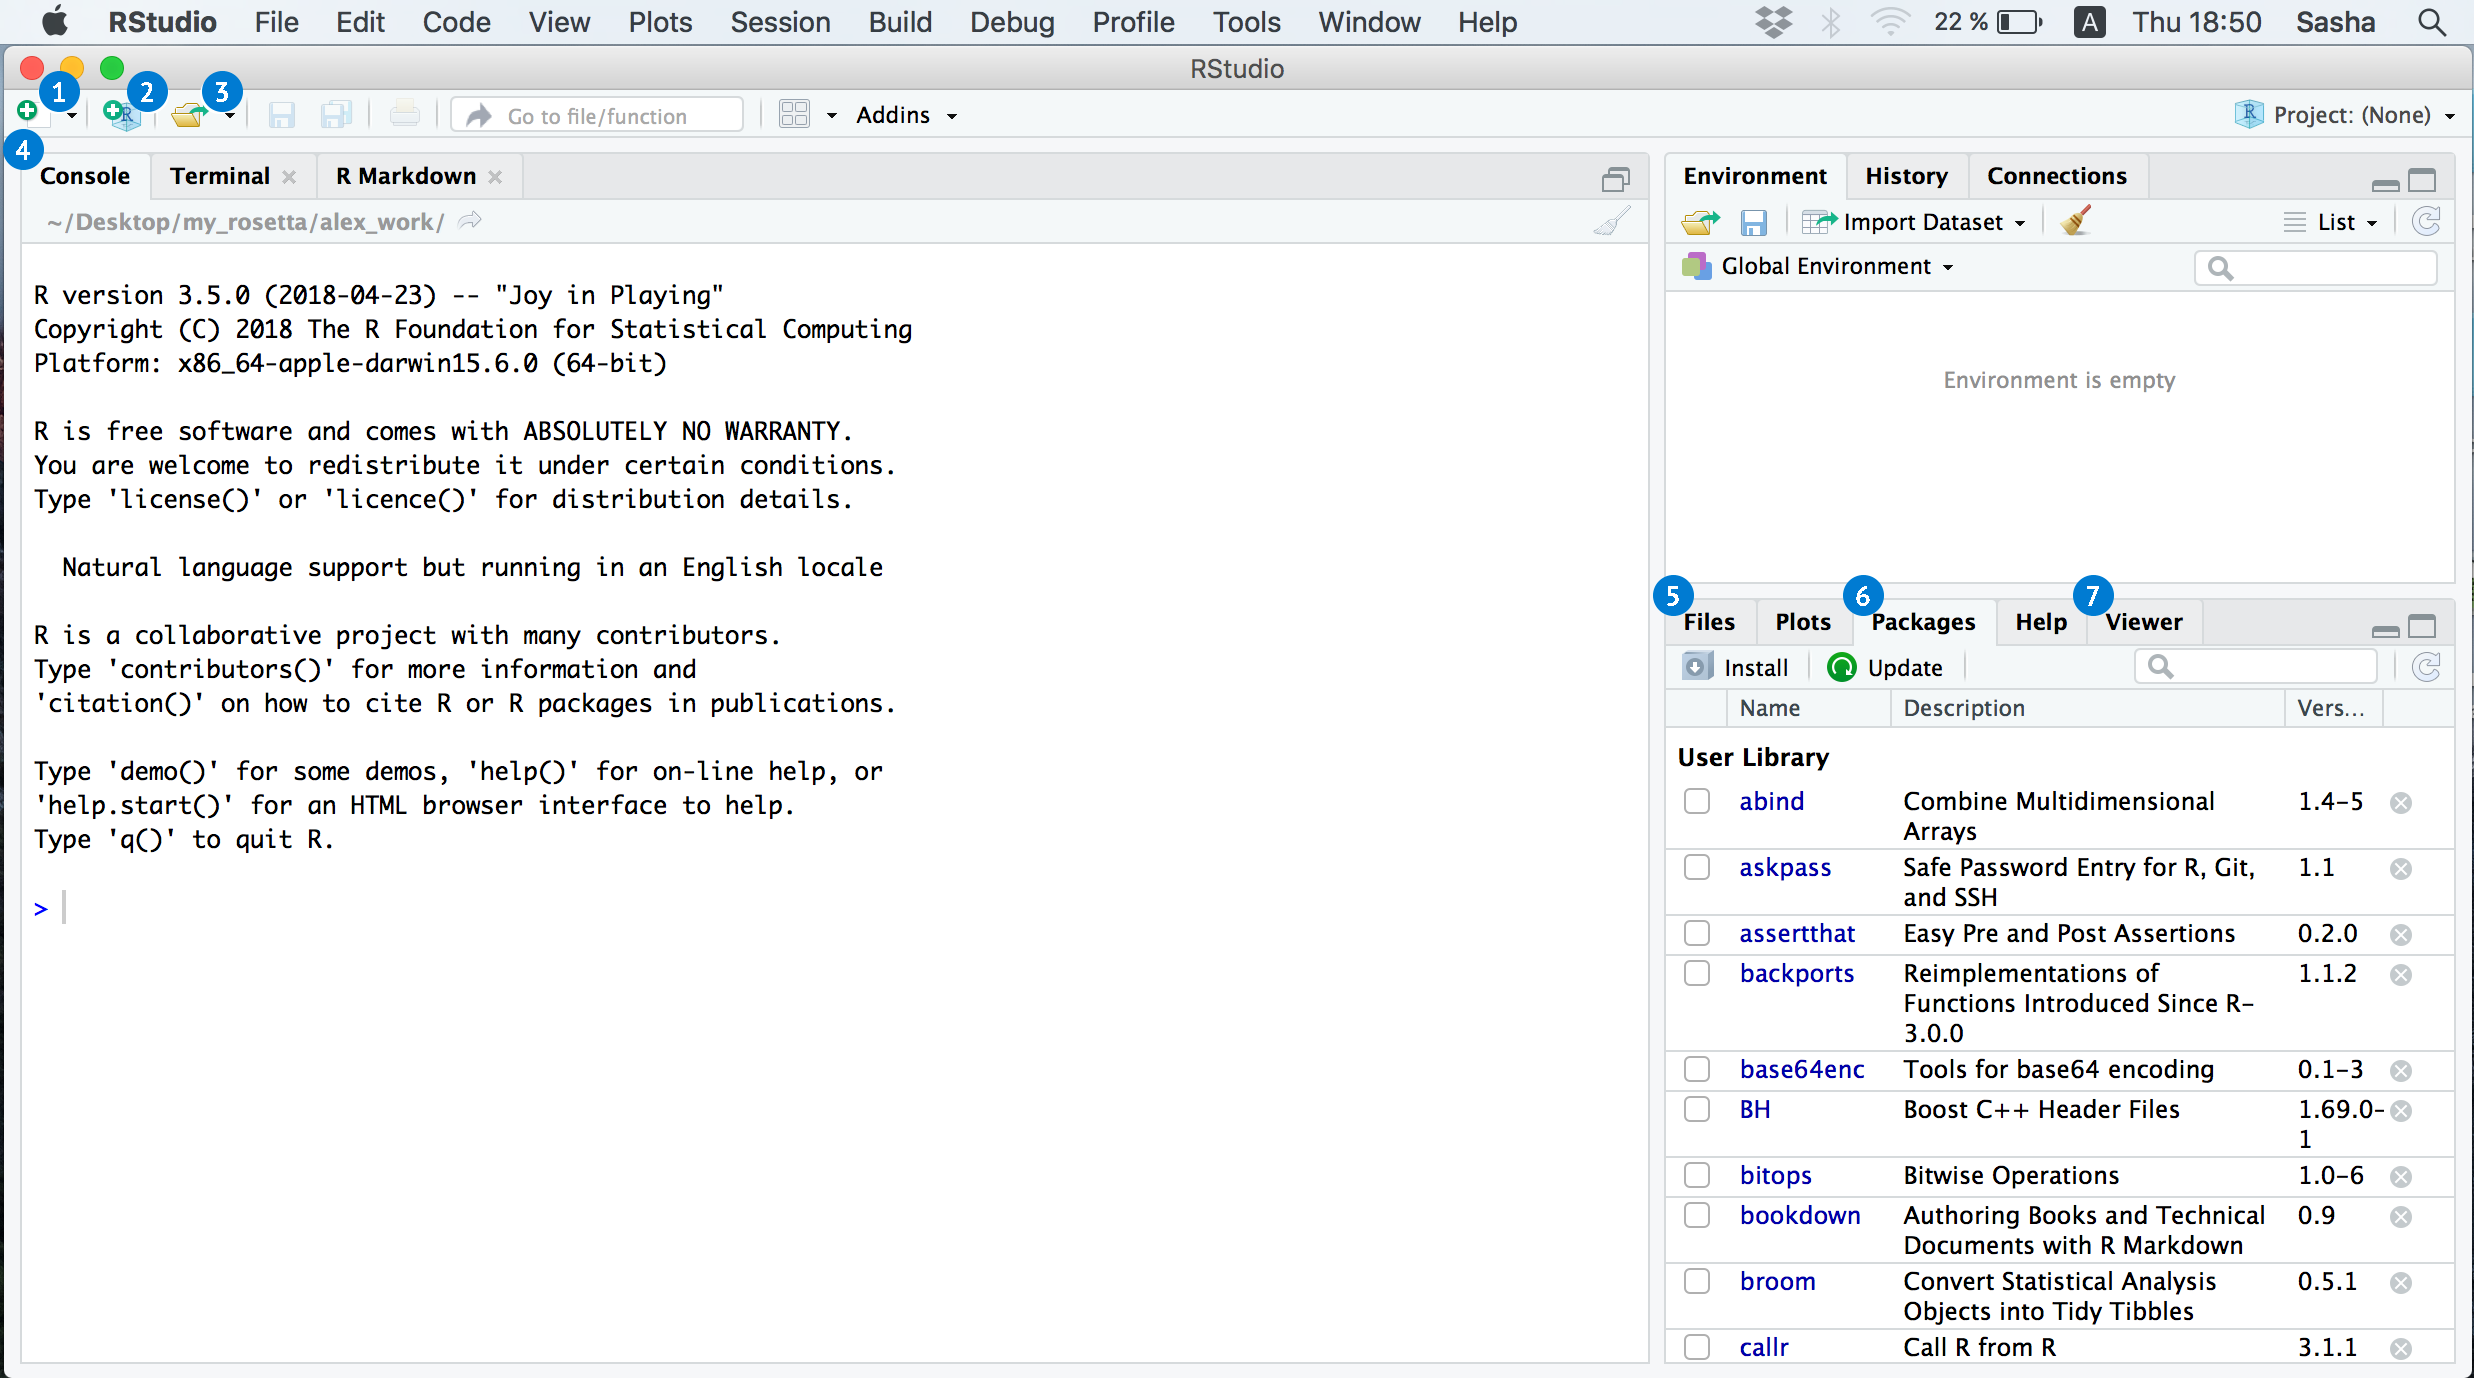
\includegraphics{images/RStudio_Interface.png}
\caption{\emph{Интерфейс программы}}
\end{figure}

\begin{enumerate}
\def\labelenumi{\arabic{enumi}.}
\item
  \textbf{New file} - Создание нового файла.
\item
  \textbf{New project} - Создание нового проекта.
\item
  \textbf{Open file} - Открытие существующего файла.
\item
  \textbf{Console} - Консоль, в которой набирается код.
\item
  \textbf{Files} - Список файлов, доступных для работы.
\item
  \textbf{Packages} - Список установленных пакетов, т.е. расширений. Также можно ознакомиться с ним, введя в консоль команду \emph{installed.packages()}.
\item
  \textbf{Viewer} - Отображение введенного кода.
\end{enumerate}

\begin{center}\rule{0.5\linewidth}{\linethickness}\end{center}

\#\#\#Язык программирования Python
\textgreater{} Python - это ещё одна открытая среда программирования, помогающая в работе со статистическими данными. Для программирования на Python подойдет программа Jupyter Notebook.

\#\#\#\#\#Установка

\begin{enumerate}
\def\labelenumi{\arabic{enumi}.}
\item
  Загрузите и установите Anaconda \href{https://www.anaconda.com/distribution/}{с официального сайта}.
\item
  После загрузки и установки откройте Anaconda Navigator, через который Вы сможете открыть программу Jupyter Notebook.
  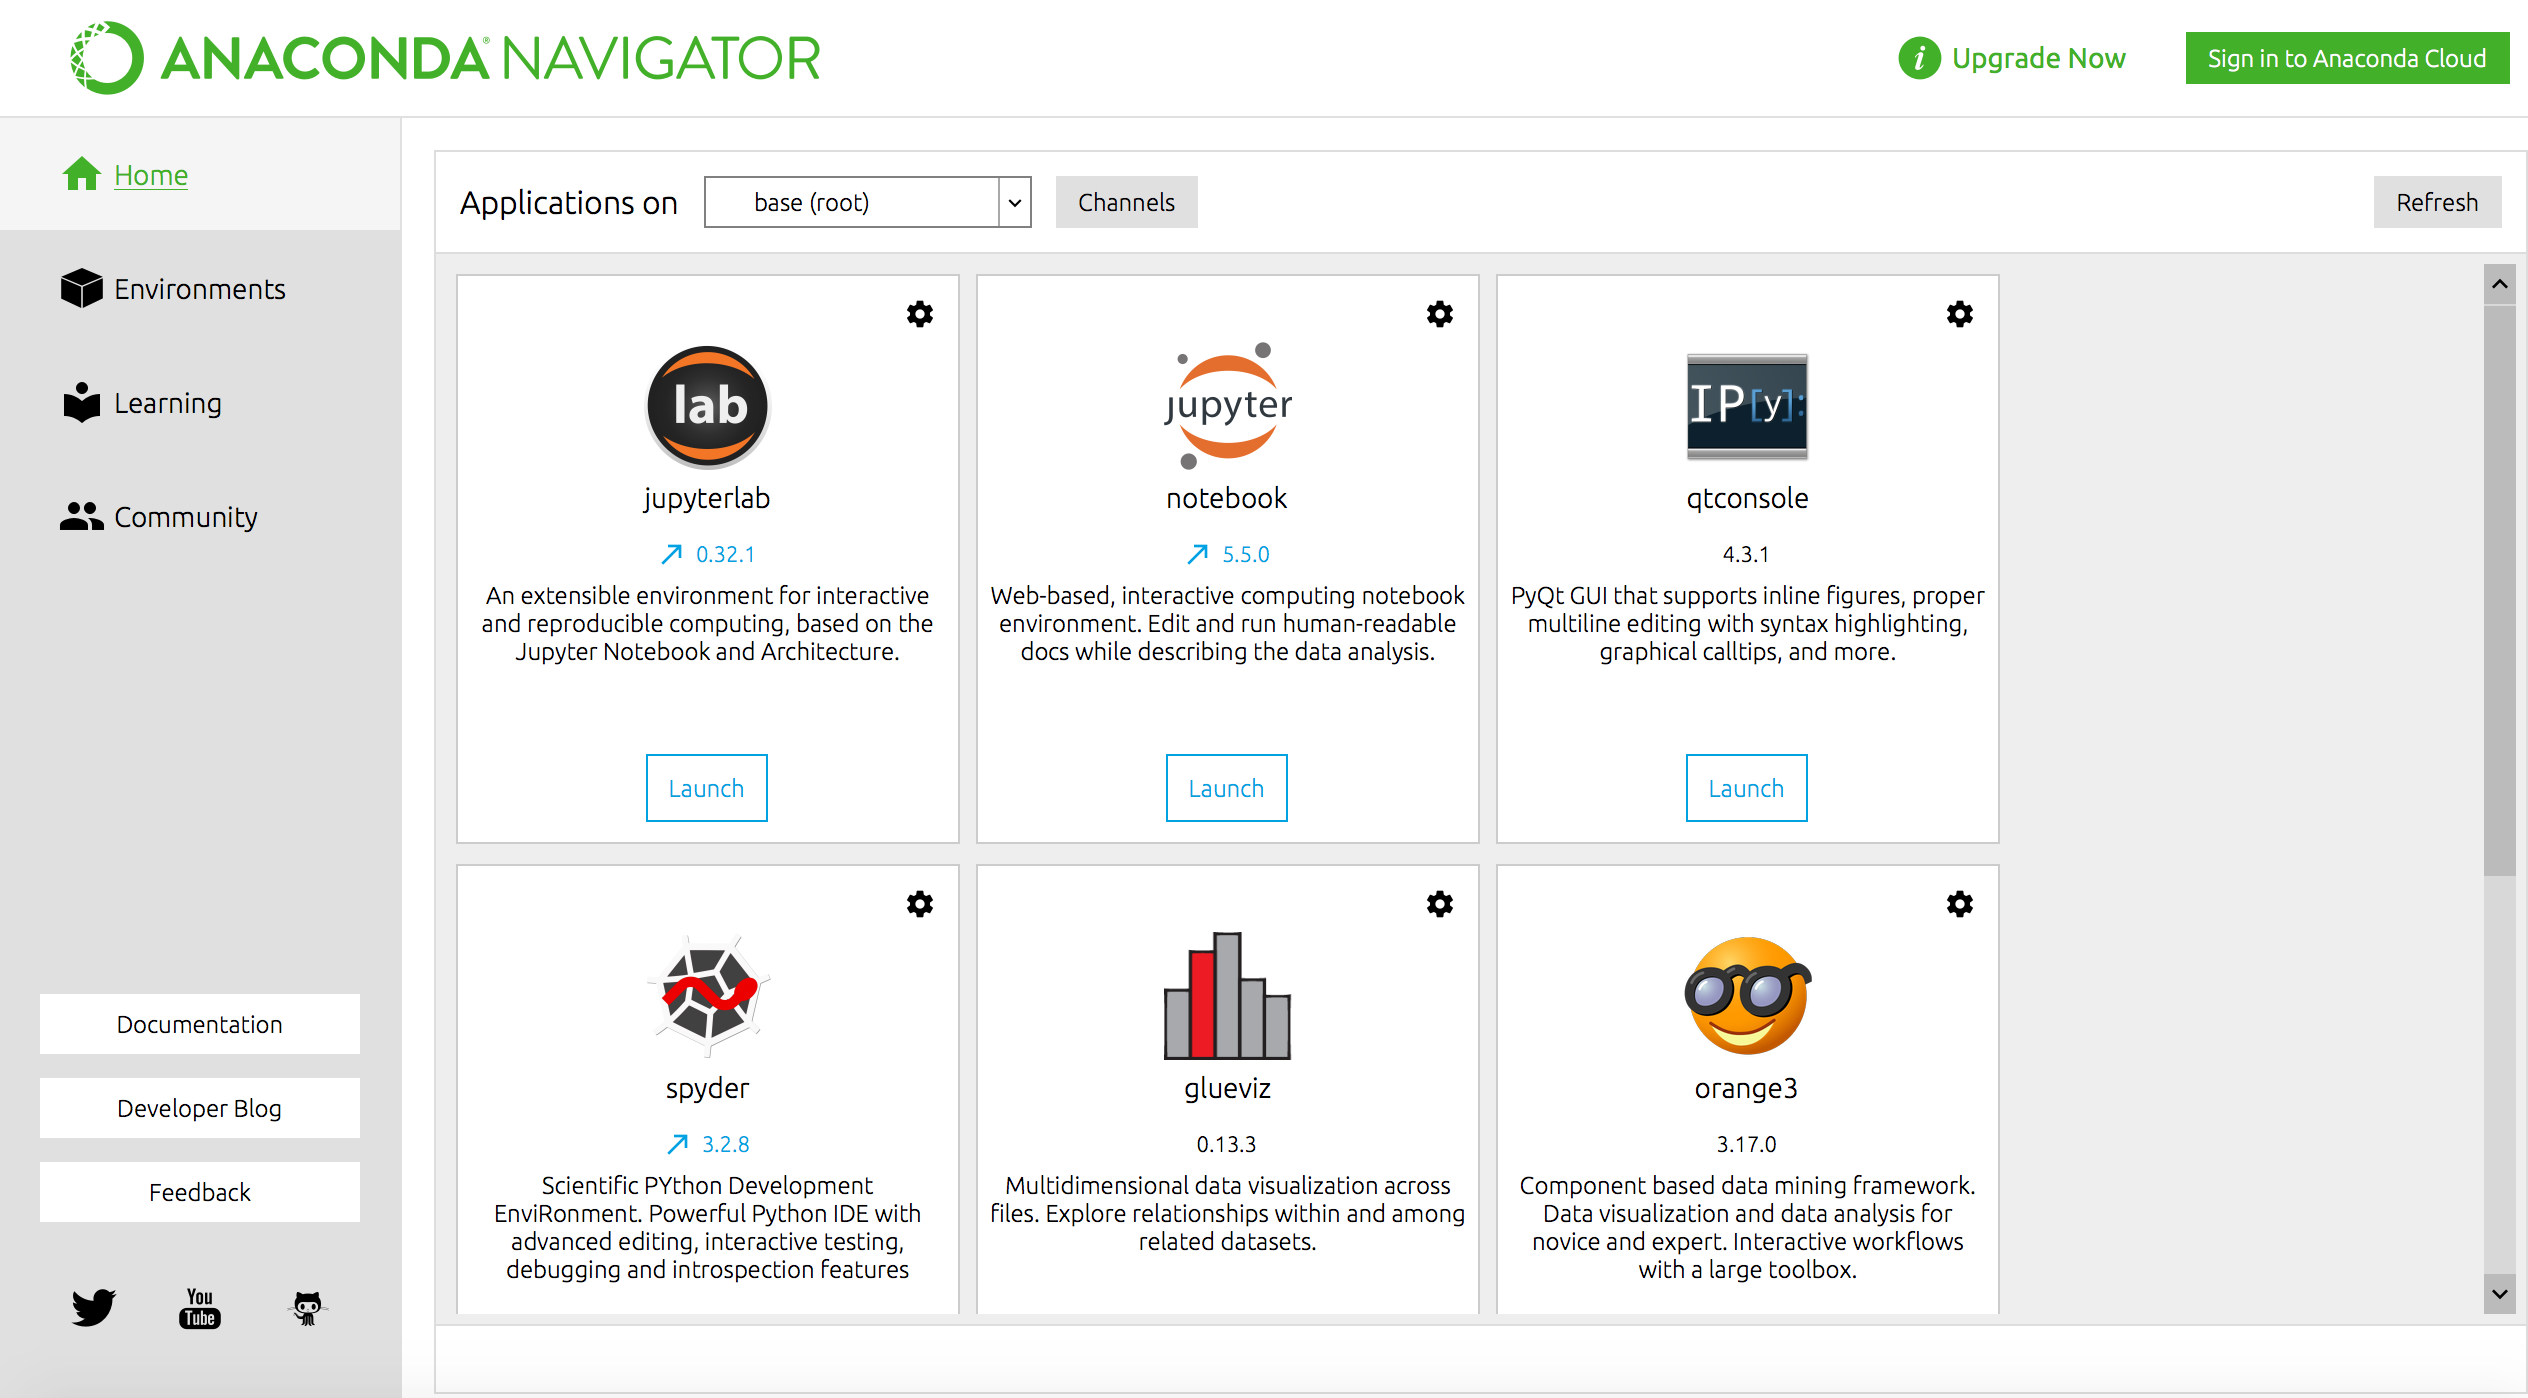
\includegraphics{images/Anaconda Navigator.png}
\end{enumerate}

\#\#\#\#\#Начало работы

Открыв Jupyter Notebook, вы попадете на страницу, содержащую ваши сохраненные файлы. Чтобы создать новый файл, нажмите ``New'' ▶ ``Notebook: Python 3''.
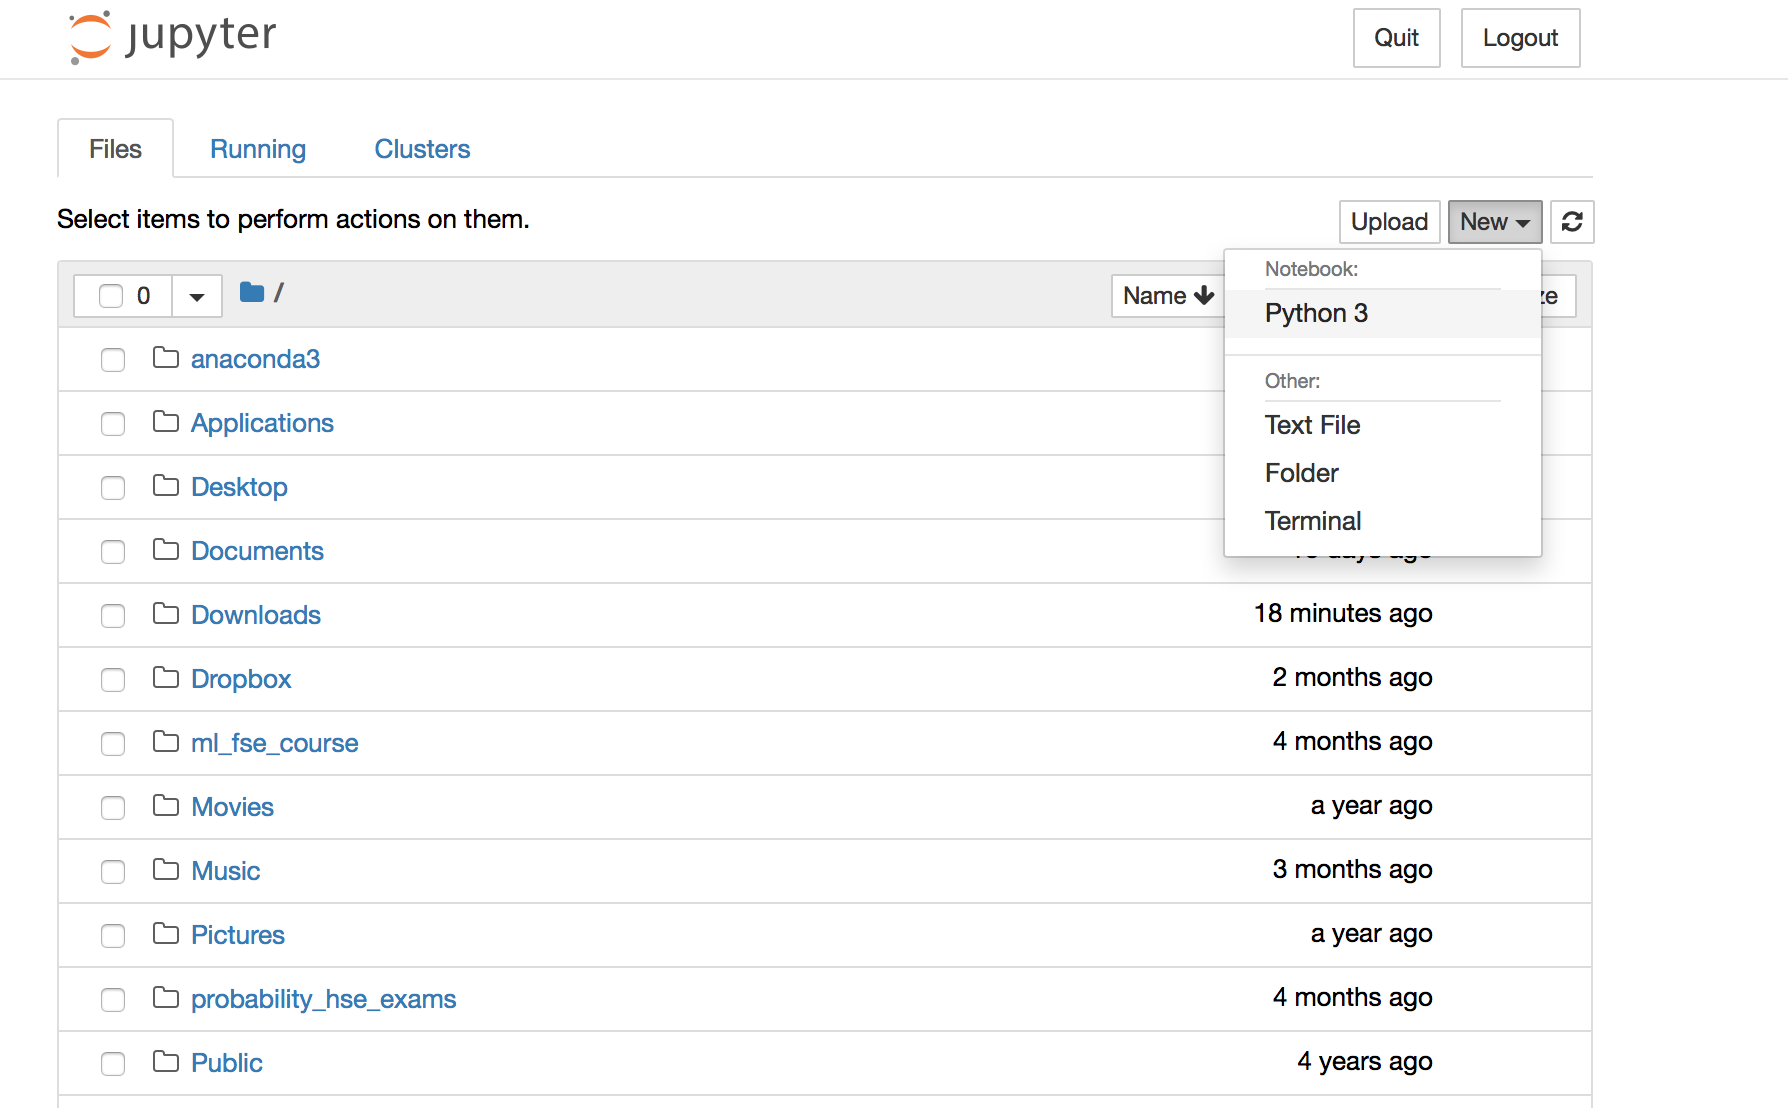
\includegraphics{images/New File in Jupyter.png}

Затем, в открывшемся окне, появится новый файл. Теперь все готово к работе. Вы можете вводить свой код и затем, используя комбинацию клавиш ``Shift'' + ``Enter'', проверять его исполнение.
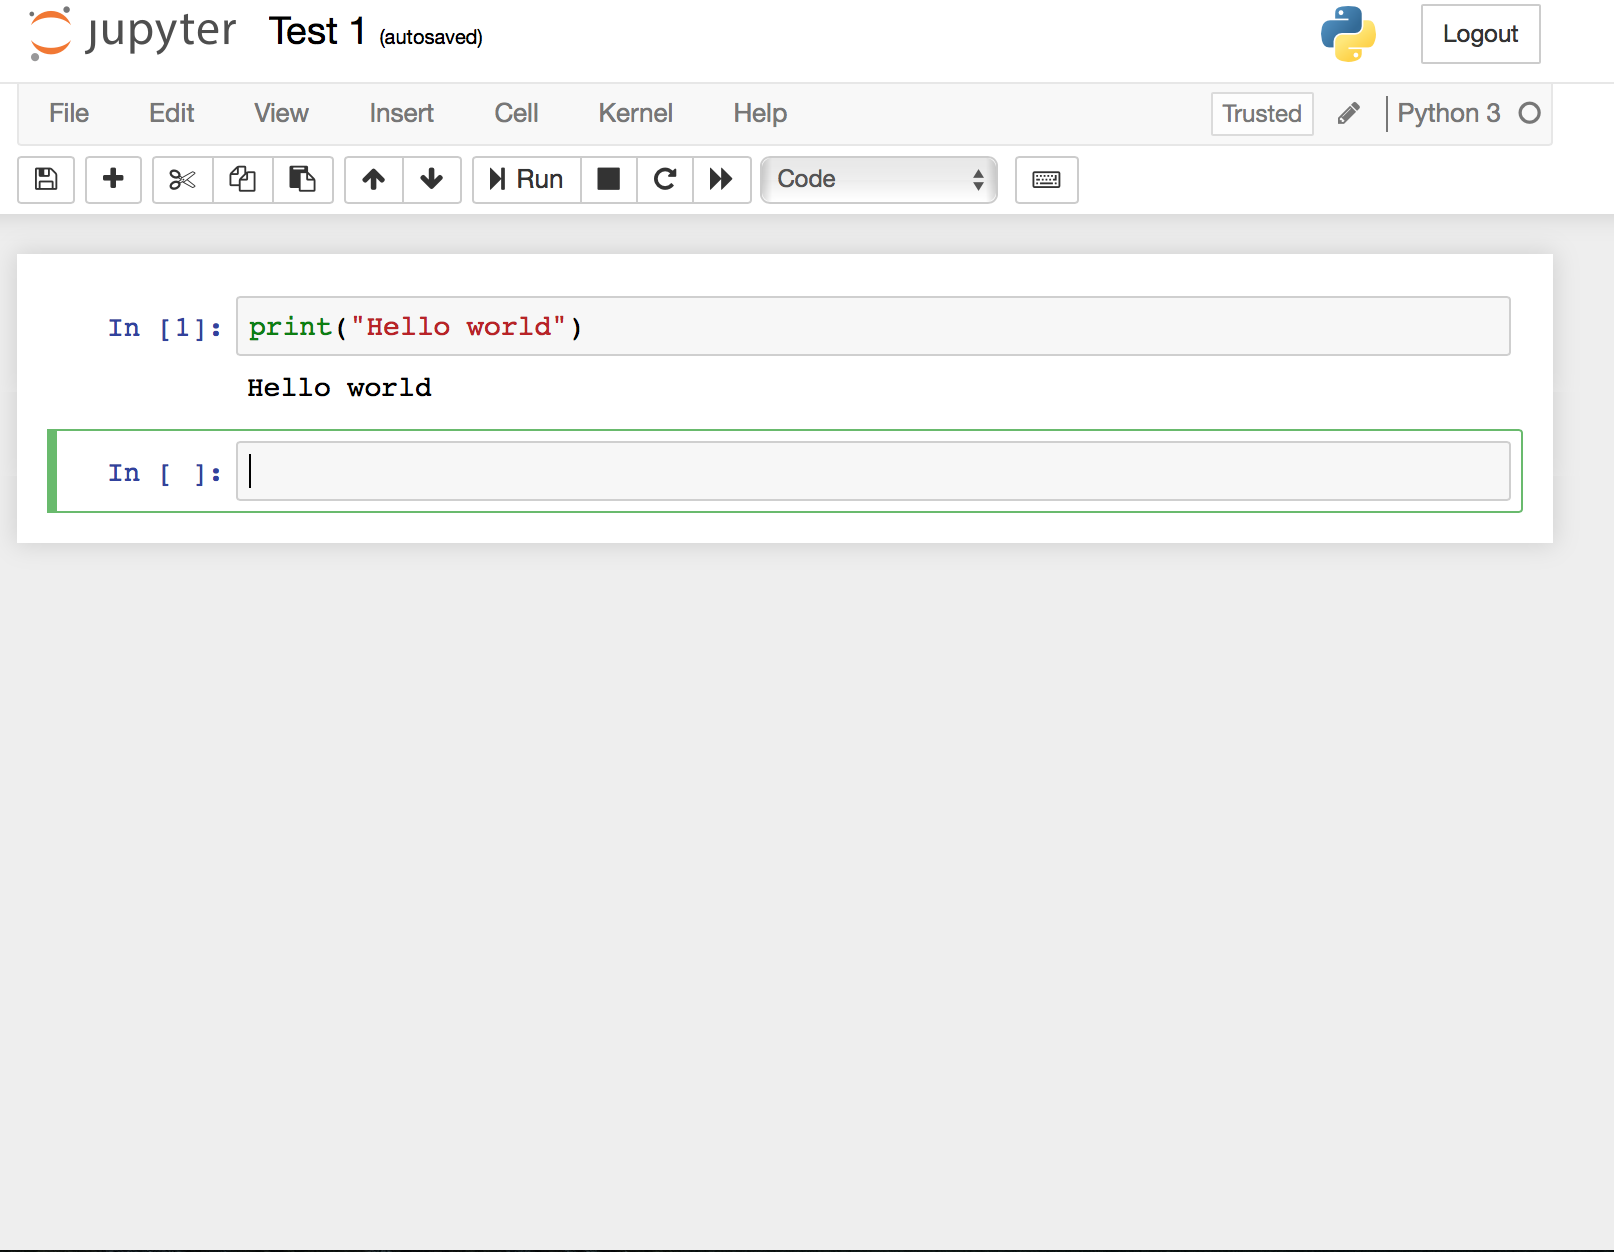
\includegraphics{images/Code in Jupyter.png}

\begin{center}\rule{0.5\linewidth}{\linethickness}\end{center}

\#\#\#Программа STATA
\textgreater{} Stata, в отличие от R и Python, является программой, а не языком программирования. Она также помогает в работе со статистическими данными.

\#\#\#\#\#Установка:

Для установки Stata необходимо загрузить актуальную версию \href{https://www.stata.com/}{с сайта компании-разработчика}. Подойдут как Stata SE, так и Stata MP.

\#\#\#\#\#Начало работы:

\begin{figure}
\centering
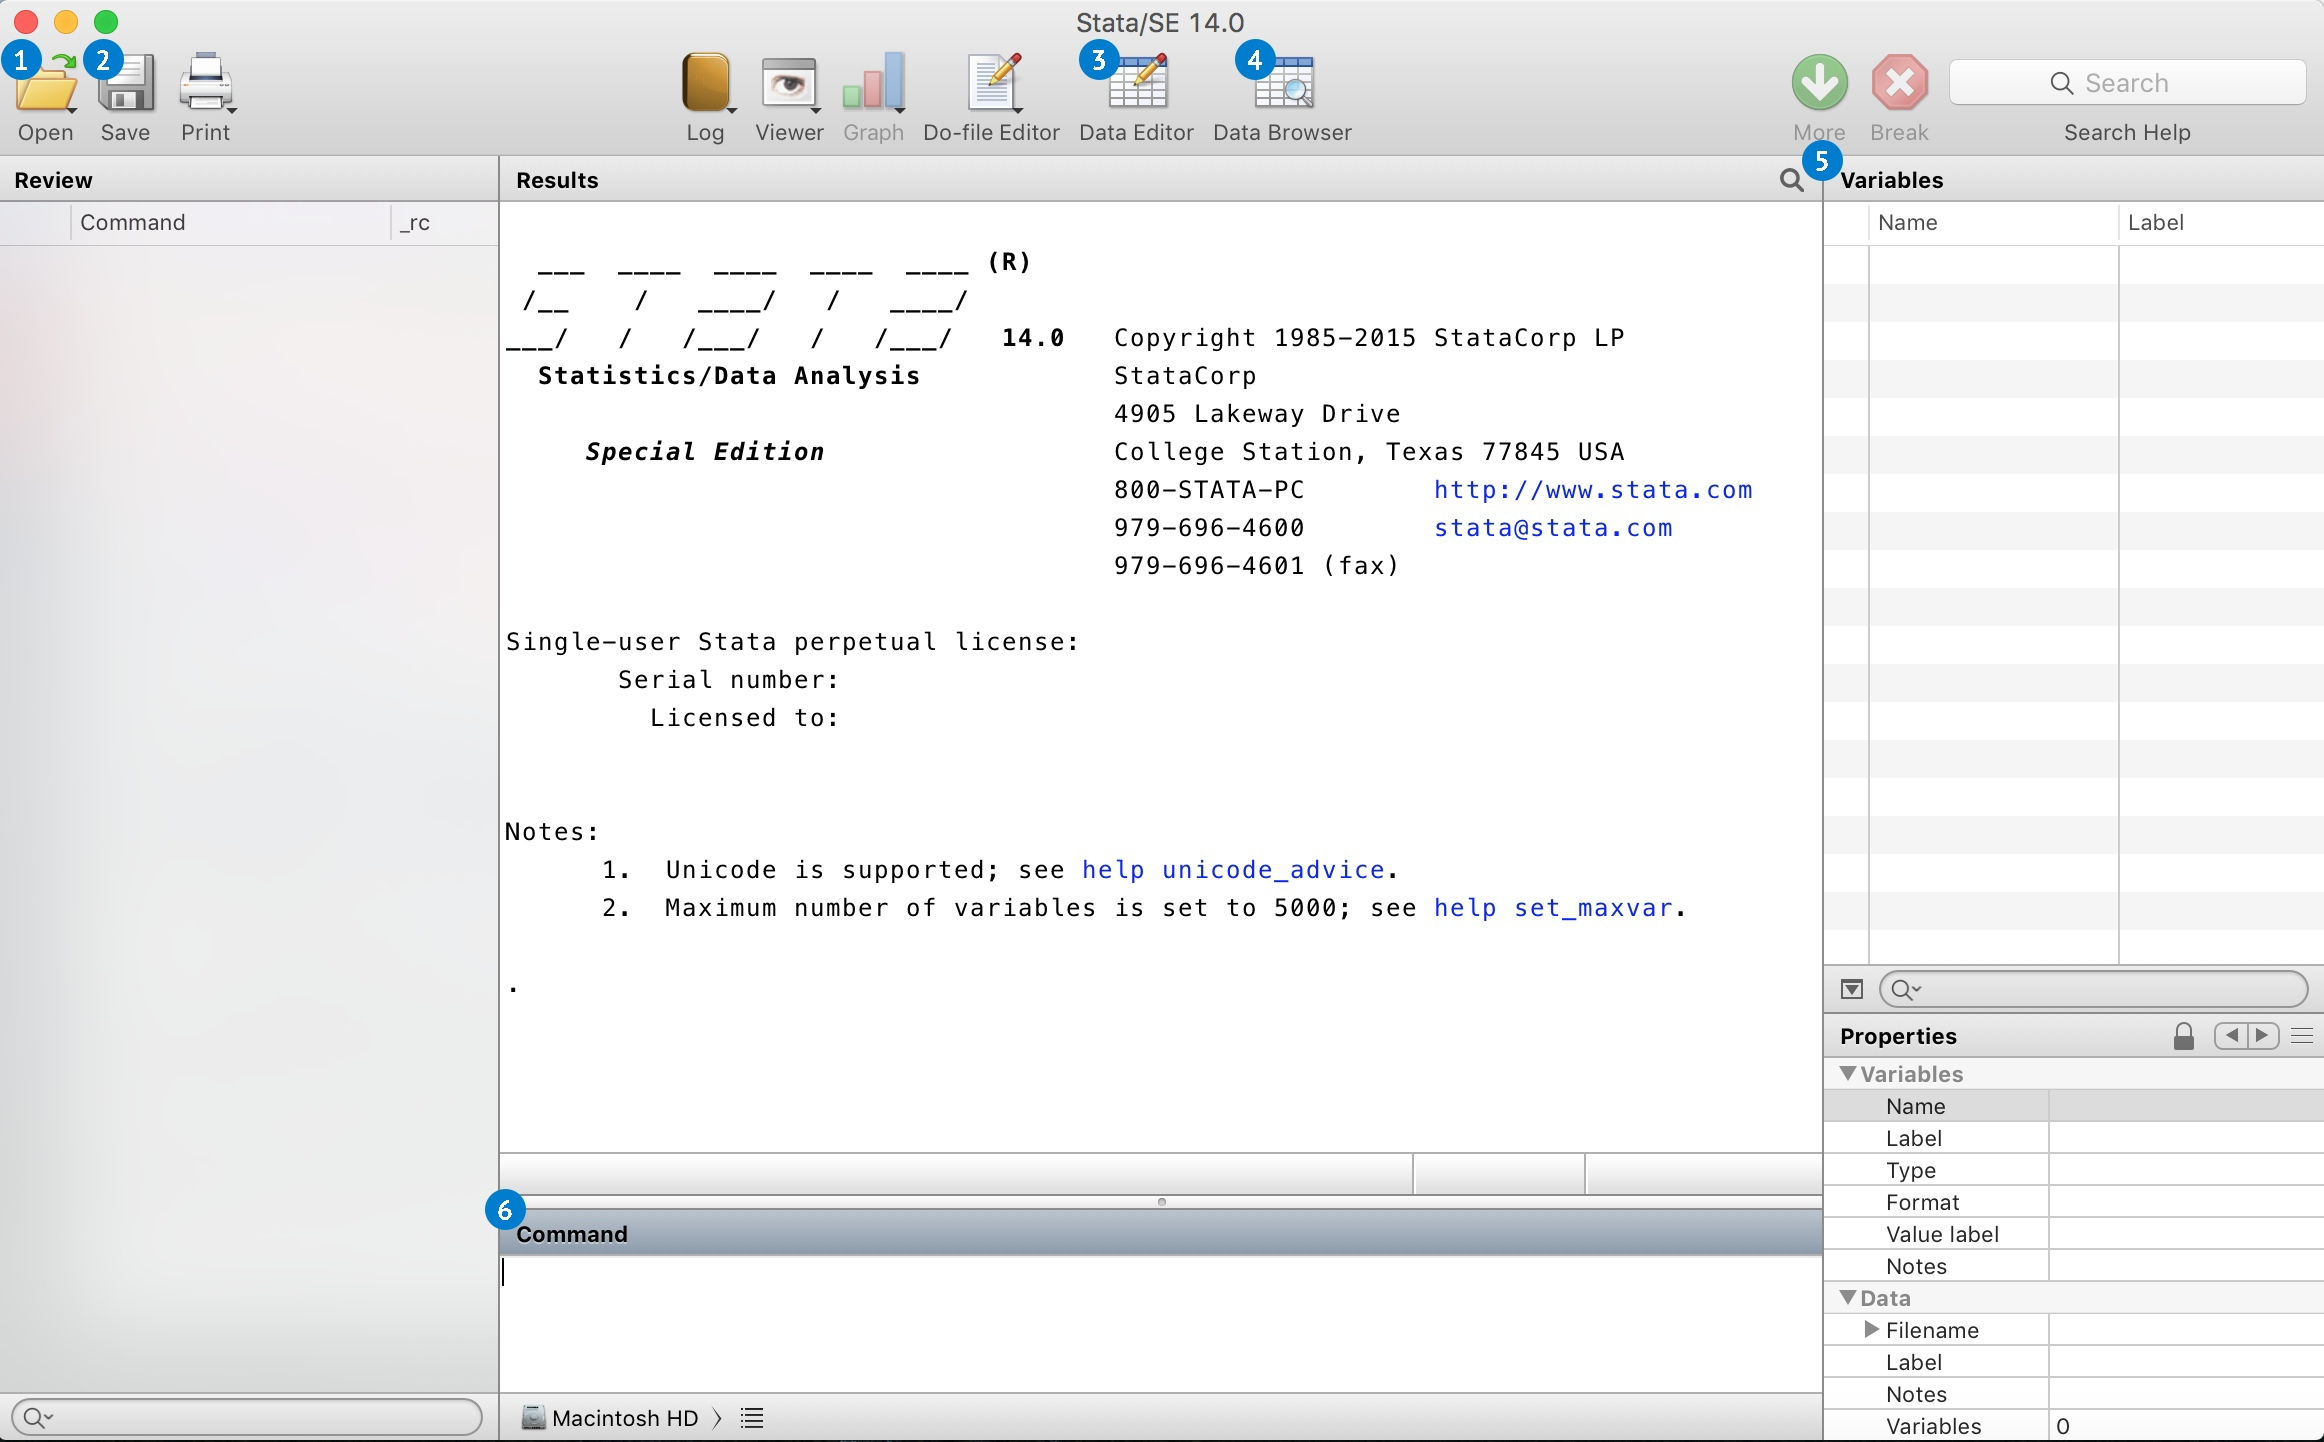
\includegraphics{images/Stata Interface.jpg}
\caption{\emph{Интерфейс Stata}}
\end{figure}

\begin{enumerate}
\def\labelenumi{\arabic{enumi}.}
\tightlist
\item
  \textbf{Open File} - открыть файл.
\item
  \textbf{Save} - сохранить файл.
\item
  \textbf{Data Editor} - редактирование данных.
\item
  \textbf{Data Browser} - просмотр данных.
\item
  \textbf{Variables} - список переменных.
\item
  \textbf{Command} - командная строка, в которой вводится код.
\end{enumerate}

\hypertarget{simplereg}{%
\chapter{Коан о простой линейной регрессии}\label{simplereg}}

\hypertarget{r}{%
\section{r}\label{r}}

Построим простую линейную регрессию в R и проведем несложные тесты.

Загрузим необходимые пакеты.

\begin{Shaded}
\begin{Highlighting}[]
\KeywordTok{library}\NormalTok{(tidyverse) }\CommentTok{# для манипуляций с данными и построения графиков}
\KeywordTok{library}\NormalTok{(skimr) }\CommentTok{# для красивого summary}
\KeywordTok{library}\NormalTok{(rio) }\CommentTok{# для чтения .dta файлов}
\KeywordTok{library}\NormalTok{(car) }\CommentTok{# для линейных гипотез}
\KeywordTok{library}\NormalTok{(tseries) }\CommentTok{# для теста на нормальность}
\KeywordTok{library}\NormalTok{(sjPlot) }\CommentTok{# еще графики}
\end{Highlighting}
\end{Shaded}

Импортируем данные.

\begin{Shaded}
\begin{Highlighting}[]
\NormalTok{df =}\StringTok{ }\NormalTok{rio}\OperatorTok{::}\KeywordTok{import}\NormalTok{(}\StringTok{"data/us-return.dta"}\NormalTok{)}
\end{Highlighting}
\end{Shaded}

Исследуем наш датасет.

\begin{Shaded}
\begin{Highlighting}[]
\KeywordTok{skim_with}\NormalTok{(}\DataTypeTok{numeric =} \KeywordTok{list}\NormalTok{(}\DataTypeTok{hist =} \OtherTok{NULL}\NormalTok{, }\DataTypeTok{p25 =} \OtherTok{NULL}\NormalTok{, }\DataTypeTok{p75 =} \OtherTok{NULL}\NormalTok{)) }\CommentTok{# опустим некоторые описательные статистики}
\KeywordTok{skim}\NormalTok{(df) }
\end{Highlighting}
\end{Shaded}

\begin{verbatim}
Skim summary statistics
 n obs: 2664 
 n variables: 22 

-- Variable type:character -----------------------------------------------------------------
 variable missing complete    n min max empty n_unique
        B       0     2664 2664   0   6  2544       31

-- Variable type:numeric -------------------------------------------------------------------
 variable missing complete    n    mean      sd      p0     p50    p100
        A    2544      120 2664 60.5    34.79    1      60.5    120    
    BOISE    2544      120 2664  0.017   0.097  -0.27    0.015    0.38 
   CITCRP    2544      120 2664  0.012   0.081  -0.28    0.011    0.32 
    CONED    2544      120 2664  0.019   0.05   -0.14    0.019    0.15 
   CONTIL    2544      120 2664 -0.0011  0.15   -0.6     0        0.97 
   DATGEN    2544      120 2664  0.0075  0.13   -0.34    0.017    0.53 
      DEC    2544      120 2664  0.02    0.099  -0.36    0.024    0.39 
    DELTA    2544      120 2664  0.012   0.096  -0.26    0.013    0.29 
   GENMIL    2544      120 2664  0.017   0.065  -0.15    0.011    0.19 
   GERBER    2544      120 2664  0.016   0.088  -0.29    0.015    0.23 
      IBM    2544      120 2664  0.0096  0.059  -0.19    0.002    0.15 
   MARKET    2544      120 2664  0.014   0.068  -0.26    0.012    0.15 
    MOBIL    2544      120 2664  0.016   0.08   -0.18    0.013    0.37 
    MOTOR    2544      120 2664  0.018   0.097  -0.33    0.017    0.27 
    PANAM    2544      120 2664  0.0035  0.13   -0.31    0        0.41 
     PSNH    2544      120 2664 -0.0042  0.11   -0.48    0        0.32 
   rkfree    2544      120 2664  0.0068  0.0022  0.0021  0.0066   0.013
   RKFREE    2544      120 2664  0.0068  0.0022  0.0021  0.0066   0.013
    TANDY    2544      120 2664  0.025   0.13   -0.25    0.022    0.45 
   TEXACO    2544      120 2664  0.012   0.08   -0.19    0.01     0.4  
    WEYER    2544      120 2664  0.0096  0.085  -0.27   -0.002    0.27 
\end{verbatim}

Переименуем столбцы.

\begin{Shaded}
\begin{Highlighting}[]
\NormalTok{df =}\StringTok{ }\KeywordTok{rename}\NormalTok{(df, }\DataTypeTok{n =}\NormalTok{ A, }\DataTypeTok{date =}\NormalTok{ B) }
\end{Highlighting}
\end{Shaded}

\begin{Shaded}
\begin{Highlighting}[]
\NormalTok{df =}\StringTok{ }\KeywordTok{na.omit}\NormalTok{(df) }\CommentTok{# уберем пустые строки}
\end{Highlighting}
\end{Shaded}

Будем верить в CAPM :) Оценим параметры модели для компании MOTOR. Соответственно, зависимая переменная - разница доходностей акций MOTOR и безрискового актива, а регрессор - рыночная премия.

\begin{Shaded}
\begin{Highlighting}[]
\NormalTok{df =}\StringTok{ }\KeywordTok{mutate}\NormalTok{(df, }\DataTypeTok{y =}\NormalTok{ MOTOR }\OperatorTok{-}\StringTok{ }\NormalTok{RKFREE, }\DataTypeTok{x =}\NormalTok{ MARKET }\OperatorTok{-}\StringTok{ }\NormalTok{RKFREE) }
\end{Highlighting}
\end{Shaded}

Строим нашу модель и проверяем гипотезу об адекватности регрессии.

\begin{Shaded}
\begin{Highlighting}[]
\NormalTok{ols =}\StringTok{ }\KeywordTok{lm}\NormalTok{(y }\OperatorTok{~}\StringTok{ }\NormalTok{x, }\DataTypeTok{data =}\NormalTok{ df)}
\KeywordTok{summary}\NormalTok{(ols)}
\end{Highlighting}
\end{Shaded}

\begin{verbatim}

Call:
lm(formula = y ~ x, data = df)

Residuals:
      Min        1Q    Median        3Q       Max 
-0.168421 -0.059381 -0.003399  0.061373  0.182991 

Coefficients:
            Estimate Std. Error t value Pr(>|t|)    
(Intercept) 0.005253   0.007200   0.730    0.467    
x           0.848150   0.104814   8.092 5.91e-13 ***
---
Signif. codes:  0 '***' 0.001 '**' 0.01 '*' 0.05 '.' 0.1 ' ' 1

Residual standard error: 0.07844 on 118 degrees of freedom
Multiple R-squared:  0.3569,    Adjusted R-squared:  0.3514 
F-statistic: 65.48 on 1 and 118 DF,  p-value: 5.913e-13
\end{verbatim}

\begin{Shaded}
\begin{Highlighting}[]
\NormalTok{coeff =}\StringTok{ }\KeywordTok{summary}\NormalTok{(ols)}\OperatorTok{$}\NormalTok{coeff }\CommentTok{# отдельно табличка с коэффициентами}
\NormalTok{coeff}
\end{Highlighting}
\end{Shaded}

\begin{verbatim}
               Estimate  Std. Error   t value     Pr(>|t|)
(Intercept) 0.005252865 0.007199935 0.7295713 4.670981e-01
x           0.848149581 0.104813757 8.0919681 5.913330e-13
\end{verbatim}

Вызовом одной функции получаем кучу полезных графиков. Можем визуально оценить наличие гетероскедастичности, нормальность распределения остатков, наличие выбросов.

\begin{Shaded}
\begin{Highlighting}[]
\KeywordTok{plot}\NormalTok{(ols)}
\end{Highlighting}
\end{Shaded}

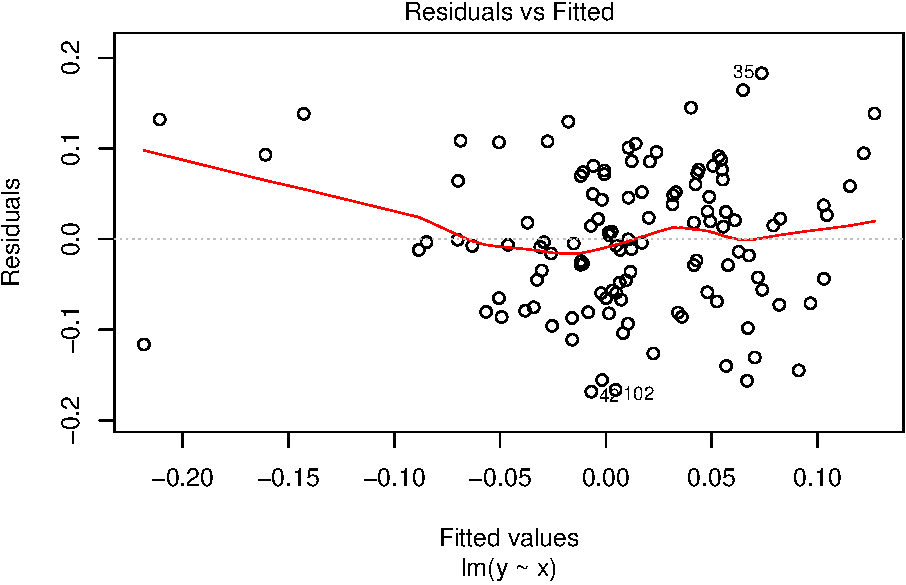
\includegraphics{02-simplereg_files/figure-latex/plot-1.pdf} 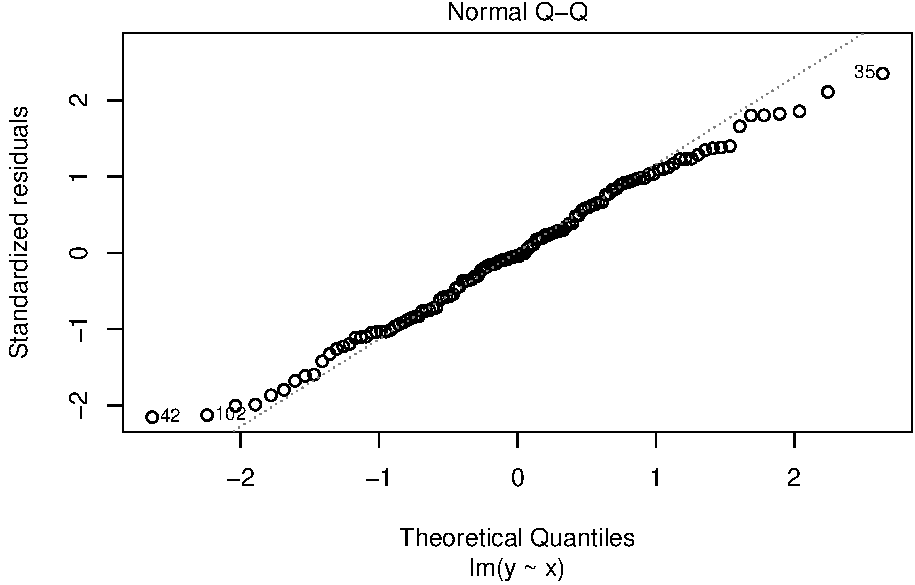
\includegraphics{02-simplereg_files/figure-latex/plot-2.pdf} 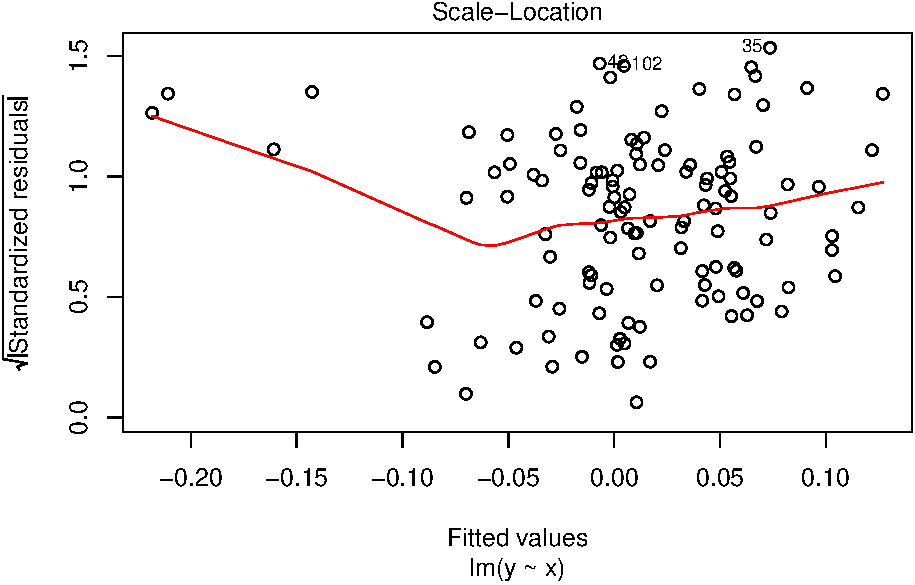
\includegraphics{02-simplereg_files/figure-latex/plot-3.pdf} 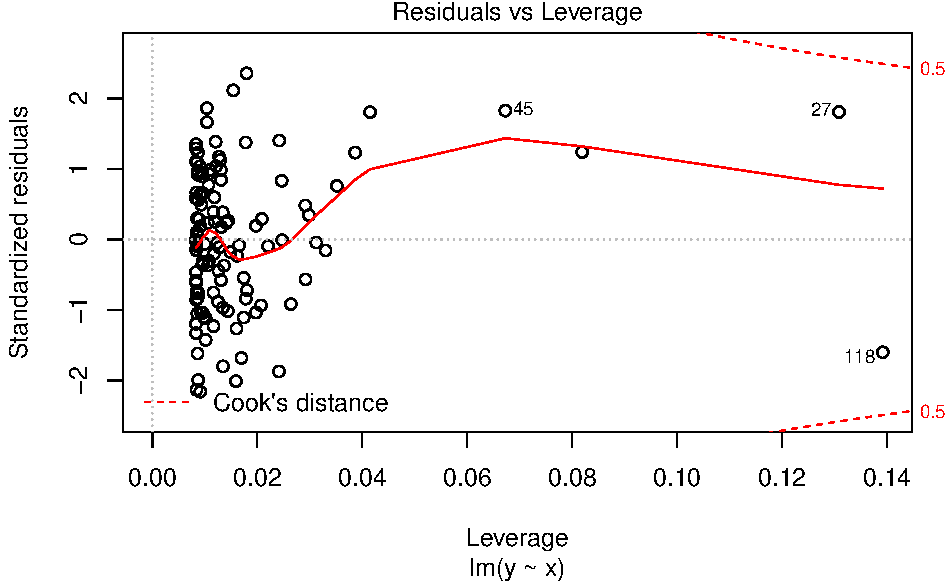
\includegraphics{02-simplereg_files/figure-latex/plot-4.pdf}

Строим доверительный интервал для параметров модели.

\begin{Shaded}
\begin{Highlighting}[]
\NormalTok{est =}\StringTok{ }\KeywordTok{cbind}\NormalTok{(}\DataTypeTok{Estimate =} \KeywordTok{coef}\NormalTok{(ols), }\KeywordTok{confint}\NormalTok{(ols))}
\end{Highlighting}
\end{Shaded}

Проверим гипотезу о равенстве коэффициента при регрессоре единице.

\begin{Shaded}
\begin{Highlighting}[]
\KeywordTok{linearHypothesis}\NormalTok{(ols, }\KeywordTok{c}\NormalTok{(}\StringTok{"x = 1"}\NormalTok{))}
\end{Highlighting}
\end{Shaded}

\begin{verbatim}
Linear hypothesis test

Hypothesis:
x = 1

Model 1: restricted model
Model 2: y ~ x

  Res.Df     RSS Df Sum of Sq      F Pr(>F)
1    119 0.73900                           
2    118 0.72608  1  0.012915 2.0989 0.1501
\end{verbatim}

Посмотрим на остатки :) Протестируем остатки регрессии на нормальность с помощью теста Харке-Бера.

\[H_{0}: S = 0, K = 3,\\
\text{где S — коэффициент асимметрии (Skewness), K — коэффициент эксцесса (Kurtosis)}\]

\begin{Shaded}
\begin{Highlighting}[]
\KeywordTok{jarque.bera.test}\NormalTok{(}\KeywordTok{resid}\NormalTok{(ols)) }
\end{Highlighting}
\end{Shaded}

\begin{verbatim}

    Jarque Bera Test

data:  resid(ols)
X-squared = 1.7803, df = 2, p-value = 0.4106
\end{verbatim}

И тест Шапиро-Уилка.

\(H_{0}: \epsilon_{i} \sim N(\mu,\sigma^2)\)

\begin{Shaded}
\begin{Highlighting}[]
\KeywordTok{shapiro.test}\NormalTok{(}\KeywordTok{resid}\NormalTok{(ols))}
\end{Highlighting}
\end{Shaded}

\begin{verbatim}

    Shapiro-Wilk normality test

data:  resid(ols)
W = 0.99021, p-value = 0.5531
\end{verbatim}

Оба теста указывают на нормальность распределения остатков регрессии.

Сделаем прогноз модели по данным вне обучаемой выборки.

\begin{Shaded}
\begin{Highlighting}[]
\KeywordTok{set.seed}\NormalTok{(}\DecValTok{7}\NormalTok{)}

\NormalTok{newData =}\StringTok{ }\KeywordTok{data.frame}\NormalTok{(}\DataTypeTok{x =}\NormalTok{ df}\OperatorTok{$}\NormalTok{x }\OperatorTok{+}\StringTok{ }\FloatTok{0.5}\OperatorTok{*}\KeywordTok{rnorm}\NormalTok{(}\KeywordTok{length}\NormalTok{(df}\OperatorTok{$}\NormalTok{x))) }\CommentTok{#пошумим}
\NormalTok{yhat =}\StringTok{ }\KeywordTok{predict}\NormalTok{(ols, }\DataTypeTok{newdata =}\NormalTok{ newData, }\DataTypeTok{se =} \OtherTok{TRUE}\NormalTok{)}
\end{Highlighting}
\end{Shaded}

\hypertarget{python}{%
\section{python}\label{python}}

Много полезных функций для статистических расчетов можно найти в пакете Statsmodels.

\begin{Shaded}
\begin{Highlighting}[]

\ImportTok{import}\NormalTok{ pandas }\ImportTok{as}\NormalTok{ pd }\CommentTok{# для работы с таблицами}
\end{Highlighting}
\end{Shaded}

\begin{verbatim}
Error in py_call_impl(callable, dots$args, dots$keywords): ModuleNotFoundError: No module named 'pandas'

Detailed traceback: 
  File "<string>", line 1, in <module>
\end{verbatim}

\begin{Shaded}
\begin{Highlighting}[]
\ImportTok{import}\NormalTok{ numpy }\ImportTok{as}\NormalTok{ np }\CommentTok{# математика, работа с матрицами}
\ImportTok{import}\NormalTok{ matplotlib.pyplot }\ImportTok{as}\NormalTok{ plt }\CommentTok{# графики}
\end{Highlighting}
\end{Shaded}

\begin{verbatim}
Error in py_call_impl(callable, dots$args, dots$keywords): ModuleNotFoundError: No module named 'matplotlib'

Detailed traceback: 
  File "<string>", line 1, in <module>
\end{verbatim}

\begin{Shaded}
\begin{Highlighting}[]
\ImportTok{import}\NormalTok{ statsmodels.api }\ImportTok{as}\NormalTok{ sm}
\end{Highlighting}
\end{Shaded}

\begin{verbatim}
Error in py_call_impl(callable, dots$args, dots$keywords): ModuleNotFoundError: No module named 'statsmodels'

Detailed traceback: 
  File "<string>", line 1, in <module>
\end{verbatim}

\begin{Shaded}
\begin{Highlighting}[]
\ImportTok{import}\NormalTok{ statsmodels.formula.api }\ImportTok{as}\NormalTok{ smf}
\end{Highlighting}
\end{Shaded}

\begin{verbatim}
Error in py_call_impl(callable, dots$args, dots$keywords): ModuleNotFoundError: No module named 'statsmodels'

Detailed traceback: 
  File "<string>", line 1, in <module>
\end{verbatim}

\begin{Shaded}
\begin{Highlighting}[]
\ImportTok{import}\NormalTok{ statsmodels.graphics.gofplots }\ImportTok{as}\NormalTok{ gf}
\end{Highlighting}
\end{Shaded}

\begin{verbatim}
Error in py_call_impl(callable, dots$args, dots$keywords): ModuleNotFoundError: No module named 'statsmodels'

Detailed traceback: 
  File "<string>", line 1, in <module>
\end{verbatim}

\begin{Shaded}
\begin{Highlighting}[]
\ImportTok{from}\NormalTok{ statsmodels.stats.outliers_influence }\ImportTok{import}\NormalTok{ summary_table}
\end{Highlighting}
\end{Shaded}

\begin{verbatim}
Error in py_call_impl(callable, dots$args, dots$keywords): ModuleNotFoundError: No module named 'statsmodels'

Detailed traceback: 
  File "<string>", line 1, in <module>
\end{verbatim}

\begin{Shaded}
\begin{Highlighting}[]
\ImportTok{import}\NormalTok{ seaborn }\ImportTok{as}\NormalTok{ sns }\CommentTok{# еще более классные графики}
\end{Highlighting}
\end{Shaded}

\begin{verbatim}
Error in py_call_impl(callable, dots$args, dots$keywords): ModuleNotFoundError: No module named 'seaborn'

Detailed traceback: 
  File "<string>", line 1, in <module>
\end{verbatim}

\begin{Shaded}
\begin{Highlighting}[]
\ImportTok{from}\NormalTok{ scipy.stats }\ImportTok{import}\NormalTok{ shapiro }\CommentTok{# еще математика}
\end{Highlighting}
\end{Shaded}

\begin{verbatim}
Error in py_call_impl(callable, dots$args, dots$keywords): ModuleNotFoundError: No module named 'scipy'

Detailed traceback: 
  File "<string>", line 1, in <module>
\end{verbatim}

\begin{Shaded}
\begin{Highlighting}[]
\ImportTok{import}\NormalTok{ statsmodels.discrete.discrete_model}
\end{Highlighting}
\end{Shaded}

\begin{verbatim}
Error in py_call_impl(callable, dots$args, dots$keywords): ModuleNotFoundError: No module named 'statsmodels'

Detailed traceback: 
  File "<string>", line 1, in <module>
\end{verbatim}

При желании, можем кастомизировать графики :)

\begin{Shaded}
\begin{Highlighting}[]
\NormalTok{plt.style.use(}\StringTok{'seaborn'}\NormalTok{)}
\end{Highlighting}
\end{Shaded}

\begin{verbatim}
Error in py_call_impl(callable, dots$args, dots$keywords): NameError: name 'plt' is not defined

Detailed traceback: 
  File "<string>", line 1, in <module>
\end{verbatim}

\begin{Shaded}
\begin{Highlighting}[]
\NormalTok{plt.rc(}\StringTok{'font'}\NormalTok{, size}\OperatorTok{=}\DecValTok{14}\NormalTok{)}
\end{Highlighting}
\end{Shaded}

\begin{verbatim}
Error in py_call_impl(callable, dots$args, dots$keywords): NameError: name 'plt' is not defined

Detailed traceback: 
  File "<string>", line 1, in <module>
\end{verbatim}

\begin{Shaded}
\begin{Highlighting}[]
\NormalTok{plt.rc(}\StringTok{'figure'}\NormalTok{, titlesize}\OperatorTok{=}\DecValTok{15}\NormalTok{)}
\end{Highlighting}
\end{Shaded}

\begin{verbatim}
Error in py_call_impl(callable, dots$args, dots$keywords): NameError: name 'plt' is not defined

Detailed traceback: 
  File "<string>", line 1, in <module>
\end{verbatim}

\begin{Shaded}
\begin{Highlighting}[]
\NormalTok{plt.rc(}\StringTok{'axes'}\NormalTok{, labelsize}\OperatorTok{=}\DecValTok{15}\NormalTok{)}
\end{Highlighting}
\end{Shaded}

\begin{verbatim}
Error in py_call_impl(callable, dots$args, dots$keywords): NameError: name 'plt' is not defined

Detailed traceback: 
  File "<string>", line 1, in <module>
\end{verbatim}

\begin{Shaded}
\begin{Highlighting}[]
\NormalTok{plt.rc(}\StringTok{'axes'}\NormalTok{, titlesize}\OperatorTok{=}\DecValTok{15}\NormalTok{)}
\end{Highlighting}
\end{Shaded}

\begin{verbatim}
Error in py_call_impl(callable, dots$args, dots$keywords): NameError: name 'plt' is not defined

Detailed traceback: 
  File "<string>", line 1, in <module>
\end{verbatim}

Загрузим данные.

\begin{Shaded}
\begin{Highlighting}[]
\NormalTok{df }\OperatorTok{=}\NormalTok{ pd.read_stata(}\StringTok{'data/us-return.dta'}\NormalTok{)}
\end{Highlighting}
\end{Shaded}

\begin{verbatim}
Error in py_call_impl(callable, dots$args, dots$keywords): NameError: name 'pd' is not defined

Detailed traceback: 
  File "<string>", line 1, in <module>
\end{verbatim}

Избавимся от наблюдений с пропущенными значениями.

\begin{Shaded}
\begin{Highlighting}[]
\NormalTok{df.dropna(inplace}\OperatorTok{=}\VariableTok{True}\NormalTok{)}
\end{Highlighting}
\end{Shaded}

\begin{verbatim}
Error in py_call_impl(callable, dots$args, dots$keywords): NameError: name 'df' is not defined

Detailed traceback: 
  File "<string>", line 1, in <module>
\end{verbatim}

\begin{Shaded}
\begin{Highlighting}[]
\NormalTok{df.reset_index(drop}\OperatorTok{=}\VariableTok{True}\NormalTok{, inplace}\OperatorTok{=}\VariableTok{True}\NormalTok{)}
\end{Highlighting}
\end{Shaded}

\begin{verbatim}
Error in py_call_impl(callable, dots$args, dots$keywords): NameError: name 'df' is not defined

Detailed traceback: 
  File "<string>", line 1, in <module>
\end{verbatim}

Переименуем столбцы.

\begin{Shaded}
\begin{Highlighting}[]
\NormalTok{df }\OperatorTok{=}\NormalTok{ df.rename(columns}\OperatorTok{=}\NormalTok{\{}\StringTok{'A'}\NormalTok{:}\StringTok{'n'}\NormalTok{, }\StringTok{'B'}\NormalTok{: }\StringTok{'date'}\NormalTok{\})}
\end{Highlighting}
\end{Shaded}

\begin{verbatim}
Error in py_call_impl(callable, dots$args, dots$keywords): NameError: name 'df' is not defined

Detailed traceback: 
  File "<string>", line 1, in <module>
\end{verbatim}

\begin{Shaded}
\begin{Highlighting}[]
\NormalTok{df[}\StringTok{'y'}\NormalTok{] }\OperatorTok{=}\NormalTok{ df[}\StringTok{'MOTOR'}\NormalTok{] }\OperatorTok{-}\NormalTok{ df[}\StringTok{'RKFREE'}\NormalTok{]}
\end{Highlighting}
\end{Shaded}

\begin{verbatim}
Error in py_call_impl(callable, dots$args, dots$keywords): NameError: name 'df' is not defined

Detailed traceback: 
  File "<string>", line 1, in <module>
\end{verbatim}

\begin{Shaded}
\begin{Highlighting}[]
\NormalTok{df[}\StringTok{'x'}\NormalTok{] }\OperatorTok{=}\NormalTok{ df[}\StringTok{'MARKET'}\NormalTok{] }\OperatorTok{-}\NormalTok{ df[}\StringTok{'RKFREE'}\NormalTok{] }
\end{Highlighting}
\end{Shaded}

\begin{verbatim}
Error in py_call_impl(callable, dots$args, dots$keywords): NameError: name 'df' is not defined

Detailed traceback: 
  File "<string>", line 1, in <module>
\end{verbatim}

Строим модель и читаем саммари :)

\begin{Shaded}
\begin{Highlighting}[]
\NormalTok{regr }\OperatorTok{=}\NormalTok{ smf.ols(}\StringTok{'y~x'}\NormalTok{, data }\OperatorTok{=}\NormalTok{ df).fit()}
\end{Highlighting}
\end{Shaded}

\begin{verbatim}
Error in py_call_impl(callable, dots$args, dots$keywords): NameError: name 'smf' is not defined

Detailed traceback: 
  File "<string>", line 1, in <module>
\end{verbatim}

\begin{Shaded}
\begin{Highlighting}[]
\NormalTok{regr.summary()}
\end{Highlighting}
\end{Shaded}

\begin{verbatim}
Error in py_call_impl(callable, dots$args, dots$keywords): NameError: name 'regr' is not defined

Detailed traceback: 
  File "<string>", line 1, in <module>
\end{verbatim}

Получить прогноз.

\begin{Shaded}
\begin{Highlighting}[]
\NormalTok{df[}\StringTok{'yhat'}\NormalTok{] }\OperatorTok{=}\NormalTok{ regr.fittedvalues}
\end{Highlighting}
\end{Shaded}

\begin{verbatim}
Error in py_call_impl(callable, dots$args, dots$keywords): NameError: name 'regr' is not defined

Detailed traceback: 
  File "<string>", line 1, in <module>
\end{verbatim}

Красивые графики для остатков, выборосов и прочих радостей, как в R, придется строить ручками. Зато приятно поиграть с оформлением :)

\begin{Shaded}
\begin{Highlighting}[]
\NormalTok{fig, ax }\OperatorTok{=}\NormalTok{ plt.subplots()}
\end{Highlighting}
\end{Shaded}

\begin{verbatim}
Error in py_call_impl(callable, dots$args, dots$keywords): NameError: name 'plt' is not defined

Detailed traceback: 
  File "<string>", line 1, in <module>
\end{verbatim}

\begin{Shaded}
\begin{Highlighting}[]
\NormalTok{ax.plot(df[}\StringTok{'x'}\NormalTok{],regr.fittedvalues, color}\OperatorTok{=}\StringTok{'g'}\NormalTok{, alpha }\OperatorTok{=}\FloatTok{0.8}\NormalTok{)}
\end{Highlighting}
\end{Shaded}

\begin{verbatim}
Error in py_call_impl(callable, dots$args, dots$keywords): NameError: name 'ax' is not defined

Detailed traceback: 
  File "<string>", line 1, in <module>
\end{verbatim}

\begin{Shaded}
\begin{Highlighting}[]
\NormalTok{ax.scatter(df[}\StringTok{'x'}\NormalTok{],regr.fittedvalues}\OperatorTok{+}\NormalTok{regr.resid, color }\OperatorTok{=} \StringTok{'g'}\NormalTok{, alpha }\OperatorTok{=} \FloatTok{0.8}\NormalTok{, s }\OperatorTok{=} \DecValTok{40}\NormalTok{)}
\end{Highlighting}
\end{Shaded}

\begin{verbatim}
Error in py_call_impl(callable, dots$args, dots$keywords): NameError: name 'ax' is not defined

Detailed traceback: 
  File "<string>", line 1, in <module>
\end{verbatim}

\begin{Shaded}
\begin{Highlighting}[]
\NormalTok{ax.vlines(df[}\StringTok{'x'}\NormalTok{],regr.fittedvalues,regr.fittedvalues}\OperatorTok{+}\NormalTok{regr.resid, color }\OperatorTok{=} \StringTok{'gray'}\NormalTok{, alpha }\OperatorTok{=} \FloatTok{0.5}\NormalTok{)}
\end{Highlighting}
\end{Shaded}

\begin{verbatim}
Error in py_call_impl(callable, dots$args, dots$keywords): NameError: name 'ax' is not defined

Detailed traceback: 
  File "<string>", line 1, in <module>
\end{verbatim}

\begin{Shaded}
\begin{Highlighting}[]
\NormalTok{plt.title(}\StringTok{'Линия регрессии и остатки'}\NormalTok{)}
\end{Highlighting}
\end{Shaded}

\begin{verbatim}
Error in py_call_impl(callable, dots$args, dots$keywords): NameError: name 'plt' is not defined

Detailed traceback: 
  File "<string>", line 1, in <module>
\end{verbatim}

\begin{Shaded}
\begin{Highlighting}[]
\NormalTok{plt.xlabel(}\StringTok{'RKFREE'}\NormalTok{)}
\end{Highlighting}
\end{Shaded}

\begin{verbatim}
Error in py_call_impl(callable, dots$args, dots$keywords): NameError: name 'plt' is not defined

Detailed traceback: 
  File "<string>", line 1, in <module>
\end{verbatim}

\begin{Shaded}
\begin{Highlighting}[]
\NormalTok{plt.ylabel(}\StringTok{'MARKET'}\NormalTok{)}
\end{Highlighting}
\end{Shaded}

\begin{verbatim}
Error in py_call_impl(callable, dots$args, dots$keywords): NameError: name 'plt' is not defined

Detailed traceback: 
  File "<string>", line 1, in <module>
\end{verbatim}

\begin{Shaded}
\begin{Highlighting}[]
\NormalTok{plt.show()}
\end{Highlighting}
\end{Shaded}

\begin{verbatim}
Error in py_call_impl(callable, dots$args, dots$keywords): NameError: name 'plt' is not defined

Detailed traceback: 
  File "<string>", line 1, in <module>
\end{verbatim}

Строим доверительный интервал.

\begin{Shaded}
\begin{Highlighting}[]
\NormalTok{regr.conf_int()}
\end{Highlighting}
\end{Shaded}

\begin{verbatim}
Error in py_call_impl(callable, dots$args, dots$keywords): NameError: name 'regr' is not defined

Detailed traceback: 
  File "<string>", line 1, in <module>
\end{verbatim}

И проведем F-test.

\begin{Shaded}
\begin{Highlighting}[]
\NormalTok{hypotheses }\OperatorTok{=} \StringTok{'(x = 1)'}
\NormalTok{regr.f_test(r_matrix }\OperatorTok{=}\NormalTok{ hypotheses)}
\end{Highlighting}
\end{Shaded}

\begin{verbatim}
Error in py_call_impl(callable, dots$args, dots$keywords): NameError: name 'regr' is not defined

Detailed traceback: 
  File "<string>", line 1, in <module>
\end{verbatim}

Тест Шапиро. Такой же, как и в R. Для удобства можно поместить в табличку.

\begin{Shaded}
\begin{Highlighting}[]
\NormalTok{W, p_value }\OperatorTok{=}\NormalTok{ shapiro(regr.resid)}
\CommentTok{#pd.DataFrame(data = \{'W': [round(W,3)], 'p_value': [round(p_value,3)]\})}
\end{Highlighting}
\end{Shaded}

\begin{verbatim}
Error in py_call_impl(callable, dots$args, dots$keywords): NameError: name 'shapiro' is not defined

Detailed traceback: 
  File "<string>", line 1, in <module>
\end{verbatim}

Генерируем новые данные и строим предсказание.

\begin{Shaded}
\begin{Highlighting}[]
\ImportTok{import}\NormalTok{ random}
\NormalTok{random.seed(}\DecValTok{7}\NormalTok{)}

\NormalTok{newData }\OperatorTok{=}\NormalTok{ df[}\StringTok{'x'}\NormalTok{] }\OperatorTok{+} \FloatTok{0.5}\OperatorTok{*}\NormalTok{np.random.normal(}\BuiltInTok{len}\NormalTok{(df))}
\end{Highlighting}
\end{Shaded}

\begin{verbatim}
Error in py_call_impl(callable, dots$args, dots$keywords): NameError: name 'df' is not defined

Detailed traceback: 
  File "<string>", line 1, in <module>
\end{verbatim}

\begin{Shaded}
\begin{Highlighting}[]
\NormalTok{prediction }\OperatorTok{=}\NormalTok{ regr.predict(newData)}
\end{Highlighting}
\end{Shaded}

\begin{verbatim}
Error in py_call_impl(callable, dots$args, dots$keywords): NameError: name 'regr' is not defined

Detailed traceback: 
  File "<string>", line 1, in <module>
\end{verbatim}

А теперь жесть! Построим графички, похожие на autoplot R.

\begin{Shaded}
\begin{Highlighting}[]
\NormalTok{fig_1 }\OperatorTok{=}\NormalTok{ plt.figure(}\DecValTok{1}\NormalTok{)}
\end{Highlighting}
\end{Shaded}

\begin{verbatim}
Error in py_call_impl(callable, dots$args, dots$keywords): NameError: name 'plt' is not defined

Detailed traceback: 
  File "<string>", line 1, in <module>
\end{verbatim}

\begin{Shaded}
\begin{Highlighting}[]
\NormalTok{fig_1.axes[}\DecValTok{0}\NormalTok{] }\OperatorTok{=}\NormalTok{ sns.residplot(df[}\StringTok{'x'}\NormalTok{], df[}\StringTok{'y'}\NormalTok{],}
\NormalTok{                                  lowess}\OperatorTok{=}\VariableTok{True}\NormalTok{,}
\NormalTok{                                  scatter_kws}\OperatorTok{=}\NormalTok{\{}\StringTok{'alpha'}\NormalTok{: }\FloatTok{0.6}\NormalTok{\},}
\NormalTok{                                  line_kws}\OperatorTok{=}\NormalTok{\{}\StringTok{'color'}\NormalTok{: }\StringTok{'red'}\NormalTok{, }\StringTok{'lw'}\NormalTok{: }\DecValTok{2}\NormalTok{, }\StringTok{'alpha'}\NormalTok{: }\FloatTok{0.8}\NormalTok{\})}
\end{Highlighting}
\end{Shaded}

\begin{verbatim}
Error in py_call_impl(callable, dots$args, dots$keywords): NameError: name 'sns' is not defined

Detailed traceback: 
  File "<string>", line 1, in <module>
\end{verbatim}

\begin{Shaded}
\begin{Highlighting}[]
\NormalTok{fig_1.axes[}\DecValTok{0}\NormalTok{].set_title(}\StringTok{'Residuals vs Fitted'}\NormalTok{)}
\end{Highlighting}
\end{Shaded}

\begin{verbatim}
Error in py_call_impl(callable, dots$args, dots$keywords): NameError: name 'fig_1' is not defined

Detailed traceback: 
  File "<string>", line 1, in <module>
\end{verbatim}

\begin{Shaded}
\begin{Highlighting}[]
\NormalTok{fig_1.axes[}\DecValTok{0}\NormalTok{].set_xlabel(}\StringTok{'Fitted values'}\NormalTok{)}
\end{Highlighting}
\end{Shaded}

\begin{verbatim}
Error in py_call_impl(callable, dots$args, dots$keywords): NameError: name 'fig_1' is not defined

Detailed traceback: 
  File "<string>", line 1, in <module>
\end{verbatim}

\begin{Shaded}
\begin{Highlighting}[]
\NormalTok{fig_1.axes[}\DecValTok{0}\NormalTok{].set_ylabel(}\StringTok{'Residuals'}\NormalTok{)}


\CommentTok{# можем добавить метки потенциальных аутлаеров}
\end{Highlighting}
\end{Shaded}

\begin{verbatim}
Error in py_call_impl(callable, dots$args, dots$keywords): NameError: name 'fig_1' is not defined

Detailed traceback: 
  File "<string>", line 1, in <module>
\end{verbatim}

\begin{Shaded}
\begin{Highlighting}[]
\NormalTok{abs_resid }\OperatorTok{=} \BuiltInTok{abs}\NormalTok{(regr.resid).sort_values(ascending}\OperatorTok{=}\VariableTok{False}\NormalTok{)}
\end{Highlighting}
\end{Shaded}

\begin{verbatim}
Error in py_call_impl(callable, dots$args, dots$keywords): NameError: name 'regr' is not defined

Detailed traceback: 
  File "<string>", line 1, in <module>
\end{verbatim}

\begin{Shaded}
\begin{Highlighting}[]
\NormalTok{abs_resid_top3 }\OperatorTok{=}\NormalTok{ abs_resid[:}\DecValTok{3}\NormalTok{]}
\end{Highlighting}
\end{Shaded}

\begin{verbatim}
Error in py_call_impl(callable, dots$args, dots$keywords): NameError: name 'abs_resid' is not defined

Detailed traceback: 
  File "<string>", line 1, in <module>
\end{verbatim}

\begin{Shaded}
\begin{Highlighting}[]
\ControlFlowTok{for}\NormalTok{ i }\KeywordTok{in}\NormalTok{ abs_resid_top3.index:}
\NormalTok{    fig_1.axes[}\DecValTok{0}\NormalTok{].annotate(i, }
\NormalTok{                               xy}\OperatorTok{=}\NormalTok{(regr.fittedvalues[i], }
\NormalTok{                                   regr.resid[i]))}
\end{Highlighting}
\end{Shaded}

\begin{verbatim}
Error in py_call_impl(callable, dots$args, dots$keywords): NameError: name 'abs_resid_top3' is not defined

Detailed traceback: 
  File "<string>", line 1, in <module>
\end{verbatim}

\begin{Shaded}
\begin{Highlighting}[]
\NormalTok{norm_residuals }\OperatorTok{=}\NormalTok{ regr.get_influence().resid_studentized_internal }\CommentTok{# сохраним стьюдентизированные остатки }
\end{Highlighting}
\end{Shaded}

\begin{verbatim}
Error in py_call_impl(callable, dots$args, dots$keywords): NameError: name 'regr' is not defined

Detailed traceback: 
  File "<string>", line 1, in <module>
\end{verbatim}

\begin{Shaded}
\begin{Highlighting}[]
\NormalTok{QQ }\OperatorTok{=}\NormalTok{ gf.ProbPlot(norm_residuals)}
\end{Highlighting}
\end{Shaded}

\begin{verbatim}
Error in py_call_impl(callable, dots$args, dots$keywords): NameError: name 'gf' is not defined

Detailed traceback: 
  File "<string>", line 1, in <module>
\end{verbatim}

\begin{Shaded}
\begin{Highlighting}[]
\NormalTok{fig_2 }\OperatorTok{=}\NormalTok{ QQ.qqplot(line}\OperatorTok{=}\StringTok{'45'}\NormalTok{, alpha}\OperatorTok{=}\FloatTok{0.5}\NormalTok{, color}\OperatorTok{=}\StringTok{'b'}\NormalTok{, lw}\OperatorTok{=}\DecValTok{1}\NormalTok{)}
\end{Highlighting}
\end{Shaded}

\begin{verbatim}
Error in py_call_impl(callable, dots$args, dots$keywords): NameError: name 'QQ' is not defined

Detailed traceback: 
  File "<string>", line 1, in <module>
\end{verbatim}

\begin{Shaded}
\begin{Highlighting}[]
\NormalTok{fig_2.axes[}\DecValTok{0}\NormalTok{].set_title(}\StringTok{'Normal Q-Q'}\NormalTok{)}
\end{Highlighting}
\end{Shaded}

\begin{verbatim}
Error in py_call_impl(callable, dots$args, dots$keywords): NameError: name 'fig_2' is not defined

Detailed traceback: 
  File "<string>", line 1, in <module>
\end{verbatim}

\begin{Shaded}
\begin{Highlighting}[]
\NormalTok{fig_2.axes[}\DecValTok{0}\NormalTok{].set_xlabel(}\StringTok{'Theoretical Quantiles'}\NormalTok{)}
\end{Highlighting}
\end{Shaded}

\begin{verbatim}
Error in py_call_impl(callable, dots$args, dots$keywords): NameError: name 'fig_2' is not defined

Detailed traceback: 
  File "<string>", line 1, in <module>
\end{verbatim}

\begin{Shaded}
\begin{Highlighting}[]
\NormalTok{fig_2.axes[}\DecValTok{0}\NormalTok{].set_ylabel(}\StringTok{'Standardized Residuals'}\NormalTok{)}\OperatorTok{;}

\CommentTok{#и снова метки}
\end{Highlighting}
\end{Shaded}

\begin{verbatim}
Error in py_call_impl(callable, dots$args, dots$keywords): NameError: name 'fig_2' is not defined

Detailed traceback: 
  File "<string>", line 1, in <module>
\end{verbatim}

\begin{Shaded}
\begin{Highlighting}[]
\NormalTok{abs_norm_resid }\OperatorTok{=}\NormalTok{ np.flip(np.argsort(}\BuiltInTok{abs}\NormalTok{(norm_residuals)), }\DecValTok{0}\NormalTok{)}
\end{Highlighting}
\end{Shaded}

\begin{verbatim}
Error in py_call_impl(callable, dots$args, dots$keywords): NameError: name 'norm_residuals' is not defined

Detailed traceback: 
  File "<string>", line 1, in <module>
\end{verbatim}

\begin{Shaded}
\begin{Highlighting}[]
\NormalTok{abs_norm_resid_top3 }\OperatorTok{=}\NormalTok{ abs_norm_resid[:}\DecValTok{3}\NormalTok{]}
\end{Highlighting}
\end{Shaded}

\begin{verbatim}
Error in py_call_impl(callable, dots$args, dots$keywords): NameError: name 'abs_norm_resid' is not defined

Detailed traceback: 
  File "<string>", line 1, in <module>
\end{verbatim}

\begin{Shaded}
\begin{Highlighting}[]
\ControlFlowTok{for}\NormalTok{ r, i }\KeywordTok{in} \BuiltInTok{enumerate}\NormalTok{(abs_norm_resid_top3):}
\NormalTok{    fig_2.axes[}\DecValTok{0}\NormalTok{].annotate(i, }
\NormalTok{                               xy}\OperatorTok{=}\NormalTok{(np.flip(QQ.theoretical_quantiles, }\DecValTok{0}\NormalTok{)[r],}
\NormalTok{                                   norm_residuals[i]))}
\end{Highlighting}
\end{Shaded}

\begin{verbatim}
Error in py_call_impl(callable, dots$args, dots$keywords): NameError: name 'abs_norm_resid_top3' is not defined

Detailed traceback: 
  File "<string>", line 1, in <module>
\end{verbatim}

\begin{Shaded}
\begin{Highlighting}[]
\NormalTok{fig_3 }\OperatorTok{=}\NormalTok{ plt.figure(}\DecValTok{3}\NormalTok{)}
\end{Highlighting}
\end{Shaded}

\begin{verbatim}
Error in py_call_impl(callable, dots$args, dots$keywords): NameError: name 'plt' is not defined

Detailed traceback: 
  File "<string>", line 1, in <module>
\end{verbatim}

\begin{Shaded}
\begin{Highlighting}[]
\NormalTok{plt.scatter(regr.fittedvalues, np.sqrt(}\BuiltInTok{abs}\NormalTok{(norm_residuals)), alpha}\OperatorTok{=}\FloatTok{0.5}\NormalTok{)}
\end{Highlighting}
\end{Shaded}

\begin{verbatim}
Error in py_call_impl(callable, dots$args, dots$keywords): NameError: name 'plt' is not defined

Detailed traceback: 
  File "<string>", line 1, in <module>
\end{verbatim}

\begin{Shaded}
\begin{Highlighting}[]
\NormalTok{sns.regplot(regr.fittedvalues, np.sqrt(}\BuiltInTok{abs}\NormalTok{(norm_residuals)), }
\NormalTok{            scatter}\OperatorTok{=}\VariableTok{False}\NormalTok{, }
\NormalTok{            ci}\OperatorTok{=}\VariableTok{False}\NormalTok{, }
\NormalTok{            lowess}\OperatorTok{=}\VariableTok{True}\NormalTok{,}
\NormalTok{            line_kws}\OperatorTok{=}\NormalTok{\{}\StringTok{'color'}\NormalTok{: }\StringTok{'red'}\NormalTok{, }\StringTok{'lw'}\NormalTok{: }\DecValTok{1}\NormalTok{, }\StringTok{'alpha'}\NormalTok{: }\FloatTok{0.6}\NormalTok{\})}
\end{Highlighting}
\end{Shaded}

\begin{verbatim}
Error in py_call_impl(callable, dots$args, dots$keywords): NameError: name 'sns' is not defined

Detailed traceback: 
  File "<string>", line 1, in <module>
\end{verbatim}

\begin{Shaded}
\begin{Highlighting}[]
\NormalTok{fig_3.axes[}\DecValTok{0}\NormalTok{].set_title(}\StringTok{'Scale-Location'}\NormalTok{)}
\end{Highlighting}
\end{Shaded}

\begin{verbatim}
Error in py_call_impl(callable, dots$args, dots$keywords): NameError: name 'fig_3' is not defined

Detailed traceback: 
  File "<string>", line 1, in <module>
\end{verbatim}

\begin{Shaded}
\begin{Highlighting}[]
\NormalTok{fig_3.axes[}\DecValTok{0}\NormalTok{].set_xlabel(}\StringTok{'Fitted values'}\NormalTok{)}
\end{Highlighting}
\end{Shaded}

\begin{verbatim}
Error in py_call_impl(callable, dots$args, dots$keywords): NameError: name 'fig_3' is not defined

Detailed traceback: 
  File "<string>", line 1, in <module>
\end{verbatim}

\begin{Shaded}
\begin{Highlighting}[]
\NormalTok{fig_3.axes[}\DecValTok{0}\NormalTok{].set_ylabel(}\StringTok{'$\textbackslash{}sqrt\{|Standardized Residuals|\}$'}\NormalTok{)}

\CommentTok{# и еще раз!)}
\end{Highlighting}
\end{Shaded}

\begin{verbatim}
Error in py_call_impl(callable, dots$args, dots$keywords): NameError: name 'fig_3' is not defined

Detailed traceback: 
  File "<string>", line 1, in <module>
\end{verbatim}

\begin{Shaded}
\begin{Highlighting}[]
\NormalTok{abs_sq_norm_resid }\OperatorTok{=}\NormalTok{ np.flip(np.argsort(np.sqrt(}\BuiltInTok{abs}\NormalTok{(norm_residuals)), }\DecValTok{0}\NormalTok{))}
\end{Highlighting}
\end{Shaded}

\begin{verbatim}
Error in py_call_impl(callable, dots$args, dots$keywords): NameError: name 'norm_residuals' is not defined

Detailed traceback: 
  File "<string>", line 1, in <module>
\end{verbatim}

\begin{Shaded}
\begin{Highlighting}[]
\NormalTok{abs_sq_norm_resid_top3 }\OperatorTok{=}\NormalTok{ abs_sq_norm_resid[:}\DecValTok{3}\NormalTok{]}
\end{Highlighting}
\end{Shaded}

\begin{verbatim}
Error in py_call_impl(callable, dots$args, dots$keywords): NameError: name 'abs_sq_norm_resid' is not defined

Detailed traceback: 
  File "<string>", line 1, in <module>
\end{verbatim}

\begin{Shaded}
\begin{Highlighting}[]
\ControlFlowTok{for}\NormalTok{ i }\KeywordTok{in}\NormalTok{ abs_sq_norm_resid_top3:}
\NormalTok{    fig_3.axes[}\DecValTok{0}\NormalTok{].annotate(i, xy}\OperatorTok{=}\NormalTok{(regr.fittedvalues[i], }
\NormalTok{                                   np.sqrt(}\BuiltInTok{abs}\NormalTok{(norm_residuals)[i])))}
\end{Highlighting}
\end{Shaded}

\begin{verbatim}
Error in py_call_impl(callable, dots$args, dots$keywords): NameError: name 'abs_sq_norm_resid_top3' is not defined

Detailed traceback: 
  File "<string>", line 1, in <module>
\end{verbatim}

\begin{Shaded}
\begin{Highlighting}[]
\NormalTok{leverage }\OperatorTok{=}\NormalTok{ regr.get_influence().hat_matrix_diag }\CommentTok{# сохраняем элементы матрицы-шляпницы}
\end{Highlighting}
\end{Shaded}

\begin{verbatim}
Error in py_call_impl(callable, dots$args, dots$keywords): NameError: name 'regr' is not defined

Detailed traceback: 
  File "<string>", line 1, in <module>
\end{verbatim}

\begin{Shaded}
\begin{Highlighting}[]
\NormalTok{cook_dist }\OperatorTok{=}\NormalTok{ regr.get_influence().cooks_distance[}\DecValTok{0}\NormalTok{] }\CommentTok{# и расстояние Кука}
\end{Highlighting}
\end{Shaded}

\begin{verbatim}
Error in py_call_impl(callable, dots$args, dots$keywords): NameError: name 'regr' is not defined

Detailed traceback: 
  File "<string>", line 1, in <module>
\end{verbatim}

\begin{Shaded}
\begin{Highlighting}[]
\NormalTok{fig_4 }\OperatorTok{=}\NormalTok{ plt.figure(}\DecValTok{4}\NormalTok{)}
\end{Highlighting}
\end{Shaded}

\begin{verbatim}
Error in py_call_impl(callable, dots$args, dots$keywords): NameError: name 'plt' is not defined

Detailed traceback: 
  File "<string>", line 1, in <module>
\end{verbatim}

\begin{Shaded}
\begin{Highlighting}[]
\NormalTok{plt.scatter(leverage, norm_residuals, alpha}\OperatorTok{=}\FloatTok{0.5}\NormalTok{)}
\end{Highlighting}
\end{Shaded}

\begin{verbatim}
Error in py_call_impl(callable, dots$args, dots$keywords): NameError: name 'plt' is not defined

Detailed traceback: 
  File "<string>", line 1, in <module>
\end{verbatim}

\begin{Shaded}
\begin{Highlighting}[]
\NormalTok{sns.regplot(leverage, norm_residuals, }
\NormalTok{            scatter}\OperatorTok{=}\VariableTok{False}\NormalTok{, }
\NormalTok{            ci}\OperatorTok{=}\VariableTok{False}\NormalTok{, }
\NormalTok{            lowess}\OperatorTok{=}\VariableTok{True}\NormalTok{,}
\NormalTok{            line_kws}\OperatorTok{=}\NormalTok{\{}\StringTok{'color'}\NormalTok{: }\StringTok{'red'}\NormalTok{, }\StringTok{'lw'}\NormalTok{: }\DecValTok{1}\NormalTok{, }\StringTok{'alpha'}\NormalTok{: }\FloatTok{0.8}\NormalTok{\})}
\end{Highlighting}
\end{Shaded}

\begin{verbatim}
Error in py_call_impl(callable, dots$args, dots$keywords): NameError: name 'sns' is not defined

Detailed traceback: 
  File "<string>", line 1, in <module>
\end{verbatim}

\begin{Shaded}
\begin{Highlighting}[]
\NormalTok{fig_4.axes[}\DecValTok{0}\NormalTok{].set_xlim(}\DecValTok{0}\NormalTok{, }\FloatTok{0.20}\NormalTok{)}
\end{Highlighting}
\end{Shaded}

\begin{verbatim}
Error in py_call_impl(callable, dots$args, dots$keywords): NameError: name 'fig_4' is not defined

Detailed traceback: 
  File "<string>", line 1, in <module>
\end{verbatim}

\begin{Shaded}
\begin{Highlighting}[]
\NormalTok{fig_4.axes[}\DecValTok{0}\NormalTok{].set_ylim(}\OperatorTok{-}\DecValTok{3}\NormalTok{, }\DecValTok{5}\NormalTok{)}
\end{Highlighting}
\end{Shaded}

\begin{verbatim}
Error in py_call_impl(callable, dots$args, dots$keywords): NameError: name 'fig_4' is not defined

Detailed traceback: 
  File "<string>", line 1, in <module>
\end{verbatim}

\begin{Shaded}
\begin{Highlighting}[]
\NormalTok{fig_4.axes[}\DecValTok{0}\NormalTok{].set_title(}\StringTok{'Residuals vs Leverage'}\NormalTok{)}
\end{Highlighting}
\end{Shaded}

\begin{verbatim}
Error in py_call_impl(callable, dots$args, dots$keywords): NameError: name 'fig_4' is not defined

Detailed traceback: 
  File "<string>", line 1, in <module>
\end{verbatim}

\begin{Shaded}
\begin{Highlighting}[]
\NormalTok{fig_4.axes[}\DecValTok{0}\NormalTok{].set_xlabel(}\StringTok{'Leverage'}\NormalTok{)}
\end{Highlighting}
\end{Shaded}

\begin{verbatim}
Error in py_call_impl(callable, dots$args, dots$keywords): NameError: name 'fig_4' is not defined

Detailed traceback: 
  File "<string>", line 1, in <module>
\end{verbatim}

\begin{Shaded}
\begin{Highlighting}[]
\NormalTok{fig_4.axes[}\DecValTok{0}\NormalTok{].set_ylabel(}\StringTok{'Standardized Residuals'}\NormalTok{)}
\end{Highlighting}
\end{Shaded}

\begin{verbatim}
Error in py_call_impl(callable, dots$args, dots$keywords): NameError: name 'fig_4' is not defined

Detailed traceback: 
  File "<string>", line 1, in <module>
\end{verbatim}

\begin{Shaded}
\begin{Highlighting}[]
\NormalTok{leverage_top3 }\OperatorTok{=}\NormalTok{ np.flip(np.argsort(cook_dist), }\DecValTok{0}\NormalTok{)[:}\DecValTok{3}\NormalTok{]}
\end{Highlighting}
\end{Shaded}

\begin{verbatim}
Error in py_call_impl(callable, dots$args, dots$keywords): NameError: name 'cook_dist' is not defined

Detailed traceback: 
  File "<string>", line 1, in <module>
\end{verbatim}

\begin{Shaded}
\begin{Highlighting}[]
\ControlFlowTok{for}\NormalTok{ i }\KeywordTok{in}\NormalTok{ leverage_top3:}
\NormalTok{    fig_4.axes[}\DecValTok{0}\NormalTok{].annotate(i, }
\NormalTok{                               xy}\OperatorTok{=}\NormalTok{(leverage[i], }
\NormalTok{                                   norm_residuals[i]))}
\end{Highlighting}
\end{Shaded}

\begin{verbatim}
Error in py_call_impl(callable, dots$args, dots$keywords): NameError: name 'leverage_top3' is not defined

Detailed traceback: 
  File "<string>", line 1, in <module>
\end{verbatim}

\begin{Shaded}
\begin{Highlighting}[]
\NormalTok{plt.show()}
\end{Highlighting}
\end{Shaded}

\begin{verbatim}
Error in py_call_impl(callable, dots$args, dots$keywords): NameError: name 'plt' is not defined

Detailed traceback: 
  File "<string>", line 1, in <module>
\end{verbatim}

\hypertarget{stata}{%
\section{stata}\label{stata}}

Загружаем данные.

\begin{verbatim}
use data/us-return.dta
\end{verbatim}

\begin{verbatim}

Любуемся и даем новые названия столбцам.

```stata
summarize
ren A n
ren B date
```

```
    Variable |        Obs        Mean    Std. Dev.       Min        Max
-------------+---------------------------------------------------------
           A |        120        60.5    34.78505          1        120
           B |          0
       MOBIL |        120    .0161917    .0803075      -.178       .366
      TEXACO |        120    .0119417    .0797036      -.194       .399
         IBM |        120    .0096167     .059024      -.187        .15
-------------+---------------------------------------------------------
         DEC |        120      .01975    .0991438      -.364       .385
      DATGEN |        120    .0074833    .1275399      -.342       .528
       CONED |        120    .0185083    .0502719      -.139       .151
        PSNH |        120   -.0042167    .1094712      -.485       .318
       WEYER |        120    .0096333    .0850664      -.271        .27
-------------+---------------------------------------------------------
       BOISE |        120     .016675    .0974882      -.274       .379
       MOTOR |        120    .0181583    .0972656      -.331        .27
       TANDY |        120    .0250083     .127566      -.246       .454
       PANAM |        120    .0035167    .1318054      -.313       .406
       DELTA |        120    .0116917    .0959317       -.26       .289
-------------+---------------------------------------------------------
      CONTIL |        120      -.0011    .1506992        -.6       .974
      CITCRP |        120    .0118583    .0809719      -.282       .318
      GERBER |        120       .0164    .0877379      -.288       .234
      GENMIL |        120    .0165833    .0650403      -.148        .19
      MARKET |        120    .0139917    .0683532       -.26       .148
-------------+---------------------------------------------------------
      RKFREE |        120    .0068386    .0021869     .00207     .01255
      rkfree |        120    .0068386    .0021869     .00207     .01255

```

Убираем пропущенные значения и создаем новые переменные.

```stata
drop if n == .
gen y = MOTOR - RKFREE
gen x = MARKET - RKFREE
```

```
(2,544 observations deleted)

```

Строим модель и проверяем гипотезу об адекватности регрессии. Тут же получаем доверительные интервалы для коэффициентов.

```stata
reg y x
```

```
      Source |       SS           df       MS      Number of obs   =       120
-------------+----------------------------------   F(1, 118)       =     65.48
       Model |  .402913404         1  .402913404   Prob > F        =    0.0000
    Residual |  .726081541       118  .006153233   R-squared       =    0.3569
-------------+----------------------------------   Adj R-squared   =    0.3514
       Total |  1.12899494       119  .009487352   Root MSE        =    .07844

------------------------------------------------------------------------------
           y |      Coef.   Std. Err.      t    P>|t|     [95% Conf. Interval]
-------------+----------------------------------------------------------------
           x |   .8481496   .1048138     8.09   0.000     .6405898    1.055709
       _cons |   .0052529   .0071999     0.73   0.467     -.009005    .0195107
------------------------------------------------------------------------------
```

Проверим гипотезу о равенстве коэффициента при регрессоре единице. 

```stata
test x = 1
```

```
 ( 1)  x = 1

       F(  1,   118) =    2.10
            Prob > F =    0.1501
```

Сделаем предсказание по выборке и сохраним остатки.

```stata
predict u_hat, resid
predict y_hat
```

```
(option xb assumed; fitted values)
```

Протестируем остатки регрессии на нормальность с помощью теста Харке-Бера.
На самом деле, это не совсем тест Харке-Бера. Оригинальный вариант ассимптотический и в нем нет поправки на размер выборки. В Stata есть. Подробнее здесь https://www.stata.com/manuals13/rsktest.pdf


```stata
sktest u_hat
```

```
                    Skewness/Kurtosis tests for Normality
                                                          ------ joint ------
    Variable |        Obs  Pr(Skewness)  Pr(Kurtosis) adj chi2(2)   Prob>chi2
-------------+---------------------------------------------------------------
       u_hat |        120     0.8841        0.1027        2.74         0.2539
```

И тест Шапиро-Уилка. Тут все аналогично R.

```stata
swilk u_hat
```

```
                   Shapiro-Wilk W test for normal data

    Variable |        Obs       W           V         z       Prob>z
-------------+------------------------------------------------------
       u_hat |        120    0.99021      0.942    -0.133    0.55310
```

Гипотеза о нормальности остатков не отвергается.

QQ - график


```stata
qnorm u_hat 
```
![](qq_plot.png)

График предсказанных значений против остатков.

```stata
rvfplot, yline(0)
```
![](resvsfit.png)

График диагональных элементов матрицы-шляпницы против квадрата остатков (по сравнению с R оси поменялись местами).

```stata
lvr2plot
```
![](resvsh.png)

График предсказанных значений против стандартизиованных остатков. Размер точек на графике зависит от расстояния Кука для данного наблюдения.

```stata
predict D, cooksd
predict standard, rstandard

graph twoway scatter standard y_hat [aweight=D], msymbol(oh) yline(0)
```
![](standardhat.png)


```stata
set seed 7

set obs 120
gen x_new = x+ 0.5 * rnormal()
gen y_hat_new =  .8481496 * x_new + .0052529 
```

```
 translator Graph2png not found
r(111);



number of observations (_N) was 120, now 120

```


<!--chapter:end:02-simplereg.Rmd-->

# Модель бинарного выбора {#binchoice}




> Сейчас попробуем подружиться с моделями бинарного выбора на основе данных `bwght.dta`, где зависимая переменная отражает, является индивид курильщиком или нет.

## r

Загрузим необходимы пакеты.

```r
library(rio) # импорт и экспорт данных в разных форматах
library(tidyverse) # графики и манипуляции с данными
library(skimr) # описательные статистики
library(mfx) # нахождение предельных эффектов
library(margins) # визуализация предельных эффектов
```

```
Error in library(margins): there is no package called 'margins'
```

```r
library(lmtest) # проведение тестов
library(plotROC) # построение ROC-кривой
```

```
Error in library(plotROC): there is no package called 'plotROC'
```

```r
library(caret) # confusion-матрица
library(texreg) # вывод результатов регрессии в тех и html
```
Импортируем исследуемые данные.

```r
data = import("data/bwght.dta") 
```

```
Error in import("data/bwght.dta"): No such file
```
Сгенерируем переменную `smoke`, отражающее состояние отдельного индивида: курильщик, если `smoke = 1`, не курильщик - иначе. 

```r
data = mutate(data, smoke=(cigs>0))
```

```
Error in UseMethod("mutate_"): no applicable method for 'mutate_' applied to an object of class "function"
```
Рассмотрим описательные статистики по всем переменным: решение курить, семейный доход, налог на сигареты, цена сигарет, образование отца и матери, паритет, цвет кожи.

```r
skim(data)
```
Заметим существование пропущенных переменных у `fatheduc`, `motheduc`. Будем анализировать только те значения, у которых нет пропущенных наблюдений. Для этого создадим новый dataframe, `data_2`, в котором отсутствуют пропущенные значения. Просмотрим его описательные статистики.

```r
data_2 = filter(data, !is.na(fatheduc), !is.na(motheduc))
```

```
Error in UseMethod("filter_"): no applicable method for 'filter_' applied to an object of class "function"
```

```r
skim(data_2)
```

```
Error in skim(data_2): object 'data_2' not found
```
Построим модель линейной вероятности. Сохраним результат под `lin_prob_model`. 

```r
lin_prob_model = lm(smoke ~ 1 + faminc + cigtax + cigprice + fatheduc + motheduc + parity + white, data=data_2)
```

```
Error in is.data.frame(data): object 'data_2' not found
```

```r
summary(lin_prob_model)
```

```
Error in summary(lin_prob_model): object 'lin_prob_model' not found
```
Посмотрим на число совпадений прогноза и исходных значений. Для этого оценим предсказанные значения модели линейной вероятности. Сохраним значение как `predictions_lin_prob_model`.

```r
predictions_lin_prob_model = predict(lin_prob_model)
```

```
Error in predict(lin_prob_model): object 'lin_prob_model' not found
```
Генерируем `smoke_ols` как 1, если вероятность по модели больше 0.5 и 0, если она меньше 0.5.

```r
smoke_ols = 1 * (predictions_lin_prob_model>0.5)
```

```
Error in eval(expr, envir, enclos): object 'predictions_lin_prob_model' not found
```
Число совпадений данных и прогноза модели линейной вероятности:

```r
sum (smoke_ols == data_2$smoke)
```

```
Error in eval(expr, envir, enclos): object 'smoke_ols' not found
```
Известно, что модель линейной вероятности обладает значительными недостатками, в частности: нереалистичное значение оцененной вероятности, ошибки, распределённые не нормально и гетероскедастичность. Поэтому оценим `P(smoke=1|x)`, и построим логит- и пробит-модели. 
Немного о логит-модели: предполагается, что существует скрытая (латентная) переменная, для которой строится модель, $$ y^*_i = \beta_1 + \beta_2 \cdot X_i + \varepsilon_i$$,так, что:

\[
\begin{equation*}
Y_i = 
 \begin{cases}
   1, &\text{если ${y_i}^* \geqslant 0$}\\
   0, &\text{если ${y_i}^* < 0$}
 \end{cases}
\end{equation*}
\]

 $$\varepsilon_i \sim logistic, \\f(t) = \frac{e^{-t}}{(1 + e^{-t})^2}$$
 
Построим логит-модель и сохраним результат оцененной модели как `logit_model`.

```r
logit_model = glm(smoke ~ 1 + faminc + cigtax + cigprice + fatheduc + motheduc + parity + white, x=TRUE, data=data_2, family=binomial(link="logit"))
```

```
Error in is.data.frame(data): object 'data_2' not found
```

```r
summary(logit_model)
```

```
Error in summary(logit_model): object 'logit_model' not found
```
Так как коэффициенты логит- и пробит- моделей плохо интерпретируются, поскольку единицы измерения латентной переменной определить сложно, посчитаем предельные эффекты, то есть изменение вероятности решения курить с изменением фактора на 1 единицу. 

Для предельного эффекта в средних значениях факторов:

```r
logitmfx(smoke ~ 1 + faminc + cigtax + cigprice + fatheduc + motheduc + parity + white, data=data_2, atmean=TRUE)
```

```
Error in is.data.frame(data): object 'data_2' not found
```

```r
margins = margins(logit_model)
```

```
Error in margins(logit_model): could not find function "margins"
```

```r
plot(margins)
```

```
Error in plot(margins): object 'margins' not found
```
Интерпретация предельных эффектов следующая (на примере переменной семейного дохода): при увеличении семейного дохода в среднем на 1 единицу при остальных неизменных факторах, вероятность стать курильщиком уменьшается в среднем на 0.18%. 

Визуализируем предельный эффект для семейного дохода:

```r
cplot(logit_model, "faminc", what="effect", main="Average Marginal Effect of Faminc")
```

```
Error in cplot(logit_model, "faminc", what = "effect", main = "Average Marginal Effect of Faminc"): could not find function "cplot"
```
Для определения качества модели построим классификационную матрицу. Для этого сначала вычислим предсказания логит-модели, `predictions_logit_model`. Так как результат не бинарный, то введём порог отсечения, равный 0.5. Назовём бинарный результат `smoke_logit`:

```r
predictions_logit_model = predict(logit_model)
```

```
Error in predict(logit_model): object 'logit_model' not found
```

```r
smoke_logit_model = (predictions_logit_model>0.5)
```

```
Error in eval(expr, envir, enclos): object 'predictions_logit_model' not found
```
Построим классификационную матрицу. При возникновении ошибок аргументов, в частности, при несовпадении их размера или типа, можно воспользоваться функцией `as.factor()`.

```r
confusionMatrix(as.factor(smoke_logit_model), as.factor(data_2$smoke))
```

```
Error in is.factor(x): object 'smoke_logit_model' not found
```
Качество модели также можно проанализировать с помощью ROC-кривой, отражающей зависимость доли верных положительно классифицируемых наблюдений (`sensitivity`) от доли ложных положительно классифицируемых наблюдений `(1-specifity)`. 

Построим ROC-кривую для логит-модели:

```r
basicplot = ggplot(data_2, aes(m=predictions_logit_model, d=data_2$smoke)) + geom_roc()
```

```
Error in ggplot(data_2, aes(m = predictions_logit_model, d = data_2$smoke)): object 'data_2' not found
```

```r
basicplot + annotate("text", x = .75, y = .25, 
           label = paste("AUC =", round(calc_auc(basicplot)$AUC, 2)))
```

```
Error in eval(expr, envir, enclos): object 'basicplot' not found
```
Площадь под кривой обозначается как AUC. Он показывает качество классификации. Соответственно, чем выше AUC, тем лучше построенная модель.

Теперь рассмотрим логит-модель, не учитывающую переменную `white`. Сохраним эту логит-модель под названием `logit_model_new`. 

```r
logit_model_new = glm(smoke ~ 1 + faminc + cigtax + cigprice + fatheduc + motheduc + parity, x=TRUE, data=data_2, family=binomial(link="logit"))
```

```
Error in is.data.frame(data): object 'data_2' not found
```
Сравним модели `logit_model` и `logit_model_new` с помощью теста максимального правдоподобия (likelihood ratio test).

```r
lrtest(logit_model,logit_model_new)
```

```
Error in lrtest(logit_model, logit_model_new): object 'logit_model' not found
```
`p-value = 0.08` в LR-тесте. Следовательно, основная гипотеза о том, что переменная `white` не влияет на решение стать курильщиком, не отвергается на 5% уровне значимости.

Сейчас посмотрим на пробит-модель. Скрытая переменная в этой модели распределена стандартно нормально: 
\[
f(t) = \frac{1 \cdot e^{\frac{-t^2}{2}}}{\sqrt{2 \cdot \pi}}
\]

Построим пробит-модель.

```r
probit_model = glm(smoke ~ 1 + faminc + cigtax + cigprice + fatheduc + motheduc + parity + white, data=data_2, family=binomial(link="probit"))
```

```
Error in is.data.frame(data): object 'data_2' not found
```

```r
summary(probit_model)
```

```
Error in summary(probit_model): object 'probit_model' not found
```
Вычисление предельных эффектов и их интерпретация, построение классификационной матрицы и ROC-кривой и LR-тест проводятся аналогично выполненным в логит-модели.
Выведем сравнительную таблицу для построенных моделей.

```r
screenreg(list(lin_prob_model, logit_model, probit_model), 
             custom.model.names = c("Модель линейной   вероятности", "Логит-модель", "Пробит-модель"))
```

```
Error in "list" %in% class(l)[1]: object 'lin_prob_model' not found
```

## python

Попробуем повторить эти шаги, используя **python**.

Импортируем пакеты:

```python
import numpy as np
import pandas as pd # чтение файлов
```

```
Error in py_call_impl(callable, dots$args, dots$keywords): ModuleNotFoundError: No module named 'pandas'

Detailed traceback: 
  File "<string>", line 1, in <module>
```

```python
import matplotlib.pyplot as plt # построение графиков
```

```
Error in py_call_impl(callable, dots$args, dots$keywords): ModuleNotFoundError: No module named 'matplotlib'

Detailed traceback: 
  File "<string>", line 1, in <module>
```

```python
from statsmodels.formula.api import logit, probit, ols # построение логит-, пробит - и линейной регрессий
```

```
Error in py_call_impl(callable, dots$args, dots$keywords): ModuleNotFoundError: No module named 'statsmodels'

Detailed traceback: 
  File "<string>", line 1, in <module>
```

```python
import statistics # описательные статистики
import sklearn
```

```
Error in py_call_impl(callable, dots$args, dots$keywords): ModuleNotFoundError: No module named 'sklearn'

Detailed traceback: 
  File "<string>", line 1, in <module>
```

```python
from sklearn import metrics # для работы с классификационными матрицами
```

```
Error in py_call_impl(callable, dots$args, dots$keywords): ModuleNotFoundError: No module named 'sklearn'

Detailed traceback: 
  File "<string>", line 1, in <module>
```

```python
from sklearn.metrics import roc_curve, auc  # ROC-curve и AUC
```

```
Error in py_call_impl(callable, dots$args, dots$keywords): ModuleNotFoundError: No module named 'sklearn'

Detailed traceback: 
  File "<string>", line 1, in <module>
```

```python
from scipy.stats.distributions import chi2 # хи-квадрат-статистика
```

```
Error in py_call_impl(callable, dots$args, dots$keywords): ModuleNotFoundError: No module named 'scipy'

Detailed traceback: 
  File "<string>", line 1, in <module>
```
Загрузим данные:

```python
data = pd.read_stata("data/bwght.dta")
```

```
Error in py_call_impl(callable, dots$args, dots$keywords): NameError: name 'pd' is not defined

Detailed traceback: 
  File "<string>", line 1, in <module>
```
Уберём пропущенные данные.Выведем описательные статистики по данным.

```python
data_2 = data.dropna()
```

```
Error in py_call_impl(callable, dots$args, dots$keywords): NameError: name 'data' is not defined

Detailed traceback: 
  File "<string>", line 1, in <module>
```

```python
data_2.describe()
```

```
Error in py_call_impl(callable, dots$args, dots$keywords): NameError: name 'data_2' is not defined

Detailed traceback: 
  File "<string>", line 1, in <module>
```
Создадим бинарную переменную `smoke`:

```python
data_2['smoke'] = 1 * (data_2['cigs']>0)
```

```
Error in py_call_impl(callable, dots$args, dots$keywords): NameError: name 'data_2' is not defined

Detailed traceback: 
  File "<string>", line 1, in <module>
```
Построим модель линейной вероятности:

```python
lin_prob_model = ols("smoke ~ 1 + faminc + cigtax + cigprice + fatheduc + motheduc + parity + white", data_2).fit()
```

```
Error in py_call_impl(callable, dots$args, dots$keywords): NameError: name 'ols' is not defined

Detailed traceback: 
  File "<string>", line 1, in <module>
```

```python
lin_prob_model.summary()
```

```
Error in py_call_impl(callable, dots$args, dots$keywords): NameError: name 'lin_prob_model' is not defined

Detailed traceback: 
  File "<string>", line 1, in <module>
```
Создадим переменную `predictions__lin_prob_model`, равную прогнозным значениям модели линейной вероятности, и посмотрим на число совпадений исходных и прогнозных данных.

```python
predictions_lin_prob_model = lin_prob_model.predict(data_2)
```

```
Error in py_call_impl(callable, dots$args, dots$keywords): NameError: name 'lin_prob_model' is not defined

Detailed traceback: 
  File "<string>", line 1, in <module>
```

```python
data_2['smoke_ols'] = 1 * (predictions_lin_prob_model>0.5)
```

```
Error in py_call_impl(callable, dots$args, dots$keywords): NameError: name 'predictions_lin_prob_model' is not defined

Detailed traceback: 
  File "<string>", line 1, in <module>
```

```python
sum(data_2['smoke']==data_2['smoke_ols'])
```

```
Error in py_call_impl(callable, dots$args, dots$keywords): NameError: name 'data_2' is not defined

Detailed traceback: 
  File "<string>", line 1, in <module>
```
Построим логит-модель.

```python
logit_model = logit("smoke ~ 1 + faminc + cigtax + cigprice + fatheduc + motheduc + parity + white", data_2).fit()
```

```
Error in py_call_impl(callable, dots$args, dots$keywords): NameError: name 'logit' is not defined

Detailed traceback: 
  File "<string>", line 1, in <module>
```

```python
logit_model.summary()
```

```
Error in py_call_impl(callable, dots$args, dots$keywords): NameError: name 'logit_model' is not defined

Detailed traceback: 
  File "<string>", line 1, in <module>
```
Посчитаем предельные эффекты в средних значениях переменных для логистической регрессии.

```python
me_mean = logit_model.get_margeff(at='mean')
```

```
Error in py_call_impl(callable, dots$args, dots$keywords): NameError: name 'logit_model' is not defined

Detailed traceback: 
  File "<string>", line 1, in <module>
```

```python
me_mean.summary()
```

```
Error in py_call_impl(callable, dots$args, dots$keywords): NameError: name 'me_mean' is not defined

Detailed traceback: 
  File "<string>", line 1, in <module>
```

Посмотрим на точность классификации построенной логит-модели. Для этого вычислим прогнозные значения модели.


```python
predictions_logit_pred = logit_model.predict(data_2) # прогнозирование значений
```

```
Error in py_call_impl(callable, dots$args, dots$keywords): NameError: name 'logit_model' is not defined

Detailed traceback: 
  File "<string>", line 1, in <module>
```

```python
data_2['smoke_logit_model'] = 1 * (predictions_logit_pred>0.5)
```

```
Error in py_call_impl(callable, dots$args, dots$keywords): NameError: name 'predictions_logit_pred' is not defined

Detailed traceback: 
  File "<string>", line 1, in <module>
```
Построим классификационную матрицу.

```python
sklearn.metrics.confusion_matrix(data_2['smoke'], data_2['smoke_logit_model'])
```

```
Error in py_call_impl(callable, dots$args, dots$keywords): NameError: name 'sklearn' is not defined

Detailed traceback: 
  File "<string>", line 1, in <module>
```
Точность прогноза и классификационные данные.

```python
np.round(sklearn.metrics.accuracy_score(data_2['smoke'],data_2['smoke_logit_model']), 2)
```

```
Error in py_call_impl(callable, dots$args, dots$keywords): NameError: name 'sklearn' is not defined

Detailed traceback: 
  File "<string>", line 1, in <module>
```

```python
sklearn.metrics.classification_report(data_2['smoke'], data_2['smoke_logit_model'])
```

```
Error in py_call_impl(callable, dots$args, dots$keywords): NameError: name 'sklearn' is not defined

Detailed traceback: 
  File "<string>", line 1, in <module>
```
Выведем ROC-кривую для логит-модели.

```python
fpr, tpr, thresholds = metrics.roc_curve(data_2['smoke'], predictions_logit_pred)
```

```
Error in py_call_impl(callable, dots$args, dots$keywords): NameError: name 'metrics' is not defined

Detailed traceback: 
  File "<string>", line 1, in <module>
```

```python
auc = metrics.roc_auc_score(data_2['smoke'], predictions_logit_pred)
```

```
Error in py_call_impl(callable, dots$args, dots$keywords): NameError: name 'metrics' is not defined

Detailed traceback: 
  File "<string>", line 1, in <module>
```

```python
plt.plot(fpr,tpr,label="auc="+str(np.round(auc, 2)))
```

```
Error in py_call_impl(callable, dots$args, dots$keywords): NameError: name 'plt' is not defined

Detailed traceback: 
  File "<string>", line 1, in <module>
```

```python
plt.legend(loc=4)
```

```
Error in py_call_impl(callable, dots$args, dots$keywords): NameError: name 'plt' is not defined

Detailed traceback: 
  File "<string>", line 1, in <module>
```

```python
plt.xlabel('1-Specifity')
```

```
Error in py_call_impl(callable, dots$args, dots$keywords): NameError: name 'plt' is not defined

Detailed traceback: 
  File "<string>", line 1, in <module>
```

```python
plt.ylabel('Sensitivity')
```

```
Error in py_call_impl(callable, dots$args, dots$keywords): NameError: name 'plt' is not defined

Detailed traceback: 
  File "<string>", line 1, in <module>
```

```python
plt.title('ROC-curve')
```

```
Error in py_call_impl(callable, dots$args, dots$keywords): NameError: name 'plt' is not defined

Detailed traceback: 
  File "<string>", line 1, in <module>
```

```python
plt.show()
```

```
Error in py_call_impl(callable, dots$args, dots$keywords): NameError: name 'plt' is not defined

Detailed traceback: 
  File "<string>", line 1, in <module>
```
Построим новую логит-модель (`logit_model_new`) без учёта переменной `white`.

```python
logit_model_new = logit("smoke ~ 1 + faminc + cigtax + cigprice + fatheduc + motheduc + parity ", data_2).fit()
```

```
Error in py_call_impl(callable, dots$args, dots$keywords): NameError: name 'logit' is not defined

Detailed traceback: 
  File "<string>", line 1, in <module>
```

```python
logit_model_new.summary()
```

```
Error in py_call_impl(callable, dots$args, dots$keywords): NameError: name 'logit_model_new' is not defined

Detailed traceback: 
  File "<string>", line 1, in <module>
```
Так как на момент написания коана готовой реализации функции теста отношения правдоподобия нет, то сделаем его ручками.

```python
L1 = logit_model.llf
```

```
Error in py_call_impl(callable, dots$args, dots$keywords): NameError: name 'logit_model' is not defined

Detailed traceback: 
  File "<string>", line 1, in <module>
```

```python
L2 = logit_model_new.llf
```

```
Error in py_call_impl(callable, dots$args, dots$keywords): NameError: name 'logit_model_new' is not defined

Detailed traceback: 
  File "<string>", line 1, in <module>
```

```python
def likelihood_ratio(llmin, llmax):
    return(2*(max(llmax, llmin) - min(llmax, llmin)))
LR = likelihood_ratio (L1, L2)
```

```
Error in py_call_impl(callable, dots$args, dots$keywords): NameError: name 'L1' is not defined

Detailed traceback: 
  File "<string>", line 1, in <module>
```

```python
np.round(chi2.sf(LR, 1), 2) # расчёт p-value для теста
```

```
Error in py_call_impl(callable, dots$args, dots$keywords): NameError: name 'chi2' is not defined

Detailed traceback: 
  File "<string>", line 1, in <module>
```
Основная гипотеза о незначимости фактора `white` не отвергается на 5% уровне значимости. 
Построим пробит-модель.

```python
probit_model = probit("smoke ~ 1 + faminc + cigtax + cigprice + fatheduc + motheduc + parity + white", data_2).fit()
```

```
Error in py_call_impl(callable, dots$args, dots$keywords): NameError: name 'probit' is not defined

Detailed traceback: 
  File "<string>", line 1, in <module>
```

```python
probit_model.summary()
```

```
Error in py_call_impl(callable, dots$args, dots$keywords): NameError: name 'probit_model' is not defined

Detailed traceback: 
  File "<string>", line 1, in <module>
```
Расчёт предельных эффектов, точности классификации, визуализация ROC-кривой и проведение LR-теста проводятся аналогично операциям с логит-моделью.
Сравнение моделей.

```python
pd.DataFrame(dict(col1=lin_prob_model.params, col2=logit_model.params, col3=probit_model.params))
```

```
Error in py_call_impl(callable, dots$args, dots$keywords): NameError: name 'pd' is not defined

Detailed traceback: 
  File "<string>", line 1, in <module>
```

## stata

А сейчас познакомимся с тем, как **stata** работает с моделями бинарного выбора.

Импортируем данные.



```stata
use data/bwght.dta
```

```
file data/bwght.dta not found
r(601);

end of do-file
r(601);
```
Сгенерируем переменную `smoke`.

```stata
gen smoke = (cigs>0) if cigs != .
```

```
 file data/bwght.dta not found
r(601);


cigs not found
r(111);

end of do-file
r(111);
```
Рассмотрим описательные статистики dataframe.

```stata
sum smoke faminc cigtax cigprice fatheduc motheduc parity white
```

```
 file data/bwght.dta not found
r(601);


no variables defined
r(111);

end of do-file
r(111);
```
Уберём пропущенные наблюдения.

```stata
sum smoke faminc cigtax cigprice fatheduc motheduc parity white if fatheduc != . & motheduc != .
```

```
 file data/bwght.dta not found
r(601);


no variables defined
r(111);

end of do-file
r(111);
```
Построим модель линейной вероятности. Сохраним результат под `lin_prob_model`.

```stata
reg smoke faminc cigtax cigprice fatheduc motheduc parity white if fatheduc != . & motheduc != .
est store lin_prob_model
```

```
 file data/bwght.dta not found
r(601);


fatheduc not found
r(111);

end of do-file
r(111);
```
Посчитаем количество совпадений прогнозов и исходных значений.

```stata
predict predictions_lin_prob_model
gen smoke_ols = (predictions_lin_prob_model>0.5) if predictions_lin_prob_model != .
count if smoke_ols == smoke
tab smoke_ols smoke
```

```
 file data/bwght.dta not found
r(601);


last estimates not found
r(301);

end of do-file
r(301);
```
Построим логит-модель и сохраним результат оцененной модели как `logit_model`.

```stata
logit smoke faminc cigtax cigprice fatheduc motheduc parity white if fatheduc != . & motheduc != .
est store logit_model
```

```
 file data/bwght.dta not found
r(601);


fatheduc not found
r(111);

end of do-file
r(111);
```
Рассчитаем предельные эффекты в средних значениях переменных.

```stata
margins, dydx(*) atmeans
```

```
 file data/bwght.dta not found
r(601);


last estimates not found
r(301);

end of do-file
r(301);
```
Визуализируем предельные эффекты.

```stata
marginsplot
```
![](marginsplot1.png)

Посмотрим на точность классификации построенной логит-модели. Для этого применяется простая команда:

```stata
estat classification
```

```
 file data/bwght.dta not found
r(601);


last estimates not found
r(301);

end of do-file
r(301);
```
Построим ROC-кривую, показывающую качество классификации построенной логит-модели.

```stata
lroc
```
![](lroc.png)

попробуем построить ещё одну логит-модель без учёта фактора `white` и сохраним новую модель под именем `logit_model_new`.

```stata
logit smoke faminc cigtax cigprice fatheduc motheduc parity if fatheduc != . & motheduc != .
est store logit_model_new
```

```
 file data/bwght.dta not found
r(601);


fatheduc not found
r(111);

end of do-file
r(111);
```
Сравним `logit_model` и `logit_model_new` с помощью LR (likelihood-ratio test):

```stata
lrtest logit_model logit_model_new
```

```
 file data/bwght.dta not found
r(601);


estimation result logit_model not found
r(111);

end of do-file
r(111);
```
`p-value = 0.08` в LR-тесте. Следовательно, основная гипотеза о том, что переменная `white` не влияет на решение стать курильщиком, не отвергается на 5% уровне значимости.

Построим пробит-модель и сохраним результат оцененной модели как `probit_model`.

```stata
probit smoke faminc cigtax cigprice fatheduc motheduc parity white if fatheduc != . & motheduc != .
est store probit_model
```

```
 file data/bwght.dta not found
r(601);


fatheduc not found
r(111);

end of do-file
r(111);
```
Сравним коэффициенты построенных моделей: модели линейной вероятности, логит- и пробит-моделей.

```stata
est tab lin_prob_model logit_model probit_model
```

```
 file data/bwght.dta not found
r(601);


estimation result lin_prob_model not found
r(111);

end of do-file
r(111);
```



<!--chapter:end:03-binchoice.Rmd-->

### Модели множественного выбора {#multchoice}




Загрузим необходимые пакеты.

```r
library(tidyverse) # для манипуляций с данными и построения графиков
library(skimr) # для красивого summary
library(rio) # для чтения .dta файлов
library(margins) # для расчета предельных эффектов
```

```
Error in library(margins): there is no package called 'margins'
```

```r
library(mlogit)
```

```
Error in library(mlogit): there is no package called 'mlogit'
```

```r
library(skimr)
library(nnet)
library(questionr)
```

```
Error in library(questionr): there is no package called 'questionr'
```

```r
library(MASS)
library(survival)
library(lattice)
```

## r

Импортируем датасет. В нем находятся данные по клиентам пенсионных фондов. Нас интересует переменная `pctstck`, которая принимает три значения: 0, 50, 100 - в зависимоcти от ответа респондента на вопрос о предпочтительном способе инвестирования пенсионных накоплений.   


```r
df = rio::import("data/pension.dta")
```


```r
skim_with(numeric = list(hist = NULL, p25 = NULL, p75 = NULL)) #посмотрим на данные

skim(df)
```

```
Skim summary statistics
 n obs: 226 
 n variables: 19 

-- Variable type:numeric -------------------------------------------------------------------
 variable missing complete   n     mean      sd   p0     p50 p100
      age       0      226 226   60.7      4.29   53   60      73
    black       0      226 226    0.12     0.33    0    0       1
   choice       0      226 226    0.62     0.49    0    1       1
     educ       7      219 226   13.52     2.55    8   12      18
   female       0      226 226    0.6      0.49    0    1       1
  finc100      10      216 226    0.12     0.33    0    0       1
  finc101      10      216 226    0.065    0.25    0    0       1
   finc25      10      216 226    0.21     0.41    0    0       1
   finc35      10      216 226    0.19     0.39    0    0       1
   finc50      10      216 226    0.25     0.43    0    0       1
   finc75      10      216 226    0.12     0.33    0    0       1
       id       0      226 226 2445.09  1371.27   38 2377.5  5014
  irain89       0      226 226    0.5      0.5     0    0.5     1
  married       0      226 226    0.73     0.44    0    1       1
  pctstck       0      226 226   46.68    39.44    0   50     100
  prftshr      20      206 226    0.21     0.41    0    0       1
   pyears       8      218 226   11.39     9.61    0    9      45
 stckin89       0      226 226    0.32     0.47    0    0       1
 wealth89       0      226 226  197.91   242.09 -580  127.85 1485
```


Создадим факторную перменную и упорядочим категории. 


```r
df = mutate(df, y = factor(pctstck)) # факторная переменная
df = mutate(df, y = relevel(y, ref = 1)) # сменить базовую категорию
levels(df$y)
```

```
[1] "0"   "50"  "100"
```

Можно взглянуть на значения объясняемой переменной в разрезе какой-то другой переменной. Или посмотреть на картиночку.


```r
table(df$y, df$educ)
```

```
     
       8  9 10 11 12 13 14 15 16 17 18
  0    5  3  0  3 31  4  7  0 11  1  7
  50   1  1  0  3 34  4  6  2 14  5 14
  100  0  2  1  1 36  1  5  4  5  4  4
```

```r
tab = xtabs(~ y + educ, data = df)
prop.table(tab, 1)
```

```
     educ
y              8          9         10         11         12         13
  0   0.06944444 0.04166667 0.00000000 0.04166667 0.43055556 0.05555556
  50  0.01190476 0.01190476 0.00000000 0.03571429 0.40476190 0.04761905
  100 0.00000000 0.03174603 0.01587302 0.01587302 0.57142857 0.01587302
     educ
y             14         15         16         17         18
  0   0.09722222 0.00000000 0.15277778 0.01388889 0.09722222
  50  0.07142857 0.02380952 0.16666667 0.05952381 0.16666667
  100 0.07936508 0.06349206 0.07936508 0.06349206 0.06349206
```

```r
spineplot(tab, off = 0)
```

![](04-multinom_choice_files/figure-latex/unnamed-chunk-1-1.pdf)<!-- --> 

Построим модель множественного выбора (лог-линейная модель). 


```r
multmodel= multinom(y ~ choice+age+educ+wealth89+prftshr, data = df, reflevel = '50')
```

```
# weights:  21 (12 variable)
initial  value 220.821070 
iter  10 value 207.012642
iter  20 value 204.507792
final  value 204.507779 
converged
```

```r
summary(multmodel)
```

```
Call:
multinom(formula = y ~ choice + age + educ + wealth89 + prftshr, 
    data = df, reflevel = "50")

Coefficients:
    (Intercept)    choice         age       educ      wealth89    prftshr
50     3.777686 0.6269410 -0.10621691 0.18518113 -0.0003716626 -0.2717872
100    4.492971 0.6244954 -0.09482129 0.04644315 -0.0003548369  0.9809245

Std. Errors:
    (Intercept)    choice        age       educ     wealth89   prftshr
50     1.581691 0.3701263 0.02826469 0.06725443 0.0007365833 0.4988234
100    1.385291 0.3851273 0.02530600 0.07203058 0.0007896235 0.4396202

Residual Deviance: 409.0156 
AIC: 433.0156 
```

При необходимости можем построить модельку для подвыборки, например, только для замужних/женатых.


```r
multmodel_married = multinom(y ~ choice+age+educ+wealth89+prftshr, subset = married == 1, data = df, reflevel = '50')
```

```
# weights:  21 (12 variable)
initial  value 165.890456 
iter  10 value 152.737765
iter  20 value 149.611359
final  value 149.611069 
converged
```

```r
summary(multmodel_married)
```

```
Call:
multinom(formula = y ~ choice + age + educ + wealth89 + prftshr, 
    data = df, subset = married == 1, reflevel = "50")

Coefficients:
    (Intercept)    choice        age       educ      wealth89   prftshr
50     4.907315 1.0040978 -0.1279041 0.19054837 -0.0006204112 0.1901337
100    5.135424 0.4658502 -0.1145570 0.09046898 -0.0002127724 1.2594092

Std. Errors:
    (Intercept)    choice        age       educ     wealth89   prftshr
50     1.836616 0.4462543 0.03282248 0.07841324 0.0008456801 0.5624022
100    1.551829 0.4583930 0.02890949 0.08508466 0.0008605946 0.5228806

Residual Deviance: 299.2221 
AIC: 323.2221 
```

Быстренько прикинули значимость коэффициентов.


```r
summary(multmodel)$coefficients/summary(multmodel)$standard.errors
```

```
    (Intercept)   choice       age      educ   wealth89    prftshr
50     2.388384 1.693857 -3.757937 2.7534413 -0.5045765 -0.5448566
100    3.243342 1.621530 -3.746989 0.6447699 -0.4493748  2.2313001
```

Сохраним прогнозы.

```r
fit_values = fitted(multmodel)
```

И посчитать относительное изменение отношения шансов:

\[
\frac{P(y_{i} = j)}{P(y_{i} = 1)} = exp(x_{i}\beta)
\] - показывает изменение отношения шансов при выборе альтернативы j вместо альтернативы 0, если x изменился на единицу


```r
odds.ratio(multmodel) 
```

```
Error in odds.ratio(multmodel): could not find function "odds.ratio"
```


Можем посчитать предельные эффекты в различных квартилях. 


```r
summary(marginal_effects(multmodel)) 
```

```
Error in marginal_effects(multmodel): could not find function "marginal_effects"
```

Допустим, мы можем упорядочить наши альтернативы (например, от более рискованного способа распределения ресурсов до менее). Тогда воспользуемся моделью упорядоченного выбора.


```r
logit.polr = polr(y ~ choice+age+educ+wealth89+prftshr , data = df)
probit.polr = polr(y ~ choice+age+educ+wealth89+prftshr , data = df, method = 'probit') 


### summary(logit.polr) не работает
```


```r
fit_prob = fitted(logit.polr)
fit_log = fitted(probit.polr)
```

## stata




```stata
use data/pension.dta
```
\end{verbatim}

\begin{verbatim}
sum
\end{verbatim}

\begin{verbatim}
    Variable |        Obs        Mean    Std. Dev.       Min        Max
-------------+---------------------------------------------------------
          id |        226    2445.093    1371.271         38       5014
      pyears |        218    11.38532    9.605498          0         45
     prftshr |        206    .2087379    .4073967          0          1
      choice |        226    .6150442     .487665          0          1
      female |        226    .6017699      .49062          0          1
-------------+---------------------------------------------------------
     married |        226    .7345133    .4425723          0          1
         age |        226    60.70354    4.287002         53         73
        educ |        219    13.51598    2.554627          8         18
      finc25 |        216    .2083333    .4070598          0          1
      finc35 |        216    .1851852      .38935          0          1
-------------+---------------------------------------------------------
      finc50 |        216    .2453704    .4313061          0          1
      finc75 |        216        .125    .3314871          0          1
     finc100 |        216    .1203704      .32615          0          1
     finc101 |        216    .0648148    .2467707          0          1
    wealth89 |        226    197.9057    242.0919   -579.997   1484.997
-------------+---------------------------------------------------------
       black |        226     .119469    .3250596          0          1
    stckin89 |        226    .3185841    .4669616          0          1
     irain89 |        226          .5    .5011099          0          1
     pctstck |        226    46.68142    39.44116          0        100
\end{verbatim}

\begin{verbatim}
ren pctstck y
\end{verbatim}

\begin{verbatim}

Построим модель множественного выбора (лог-линейная модель). 

```stata
mlogit y choice age educ wealth89 prftshr,  baseoutcome(0) 
```

```
Iteration 0:   log likelihood = -219.86356  
Iteration 1:   log likelihood = -204.58172  
Iteration 2:   log likelihood =  -204.5078  
Iteration 3:   log likelihood = -204.50778  
Iteration 4:   log likelihood = -204.50778  

Multinomial logistic regression                 Number of obs     =        201
                                                LR chi2(10)       =      30.71
                                                Prob > chi2       =     0.0007
Log likelihood = -204.50778                     Pseudo R2         =     0.0698

------------------------------------------------------------------------------
           y |      Coef.   Std. Err.      z    P>|z|     [95% Conf. Interval]
-------------+----------------------------------------------------------------
0            |  (base outcome)
-------------+----------------------------------------------------------------
50           |
      choice |   .6269473   .3706065     1.69   0.091    -.0994281    1.353323
         age |  -.1062189   .0434194    -2.45   0.014    -.1913193   -.0211185
        educ |   .1851821    .070641     2.62   0.009     .0467283    .3236359
    wealth89 |  -.0003717   .0007432    -0.50   0.617    -.0018283     .001085
     prftshr |  -.2718087   .4988312    -0.54   0.586      -1.2495    .7058825
       _cons |   3.777798   2.790118     1.35   0.176    -1.690732    9.246328
-------------+----------------------------------------------------------------
100          |
      choice |   .6244907   .3859169     1.62   0.106    -.1318925    1.380874
         age |  -.0948282   .0450488    -2.11   0.035    -.1831222   -.0065341
        educ |   .0464378   .0767858     0.60   0.545    -.1040595    .1969352
    wealth89 |  -.0003548    .000797    -0.45   0.656     -.001917    .0012074
     prftshr |   .9809114   .4396226     2.23   0.026      .119267    1.842556
       _cons |   4.493463   2.967396     1.51   0.130    -1.322526    10.30945
------------------------------------------------------------------------------
```

Можем посмотреть на прогнозы.


```stata
predict p1 p2 p3, p
```

```
(25 missing values generated)
```

И посчитать относительное изменение отношения шансов:

\[
\frac{P(y_{i} = j)}{P(y_{i} = 1)} = exp(x_{i}\beta)
\] - показывает изменение отношения шансов при выборе альтернативы j вместо альтернативы 0, если x изменился на единицу.
В stata, в отличие от R, отношение шансов называется relative-risk ratio.


```stata
mlogit, rrr
```

```
Multinomial logistic regression                 Number of obs     =        201
                                                LR chi2(10)       =      30.71
                                                Prob > chi2       =     0.0007
Log likelihood = -204.50778                     Pseudo R2         =     0.0698

------------------------------------------------------------------------------
           y |        RRR   Std. Err.      z    P>|z|     [95% Conf. Interval]
-------------+----------------------------------------------------------------
0            |  (base outcome)
-------------+----------------------------------------------------------------
50           |
      choice |   1.871888   .6937337     1.69   0.091     .9053551    3.870264
         age |   .8992278   .0390439    -2.45   0.014     .8258688     .979103
        educ |   1.203438    .085012     2.62   0.009     1.047837    1.382144
    wealth89 |   .9996284   .0007429    -0.50   0.617     .9981733    1.001086
     prftshr |       .762   .3801094    -0.54   0.586     .2866481    2.025633
       _cons |   43.71966    121.983     1.35   0.176     .1843845    10366.43
-------------+----------------------------------------------------------------
100          |
      choice |   1.867295   .7206205     1.62   0.106     .8764352    3.978377
         age |   .9095292   .0409732    -2.11   0.035     .8326664    .9934872
        educ |   1.047533   .0804356     0.60   0.545     .9011717    1.217665
    wealth89 |   .9996452   .0007968    -0.45   0.656     .9980848    1.001208
     prftshr |   2.666886   1.172423     2.23   0.026     1.126671    6.312652
       _cons |   89.43064   265.3761     1.51   0.130     .2664612    30015.02
------------------------------------------------------------------------------
```


Можем посчитать предельные эффекты в разных точках.


```stata
margins, predict(outcome(50)) dydx(choice age educ wealth89 prftshr) atmeans 

margins, predict(outcome(50)) dydx(choice age educ wealth89 prftshr) at((p25) *)
```

```
Conditional marginal effects                    Number of obs     =        201
Model VCE    : OIM

Expression   : Pr(y==50), predict(outcome(50))
dy/dx w.r.t. : choice age educ wealth89 prftshr
at           : choice          =    .6069652 (mean)
               age             =    60.52736 (mean)
               educ            =    13.56219 (mean)
               wealth89        =    205.5467 (mean)
               prftshr         =    .2089552 (mean)

------------------------------------------------------------------------------
             |            Delta-method
             |      dy/dx   Std. Err.      z    P>|z|     [95% Conf. Interval]
-------------+----------------------------------------------------------------
      choice |    .077144   .0757102     1.02   0.308    -.0712453    .2255333
         age |   -.014281   .0089754    -1.59   0.112    -.0318725    .0033105
        educ |   .0380169   .0140813     2.70   0.007     .0104182    .0656157
    wealth89 |  -.0000474   .0001544    -0.31   0.759      -.00035    .0002551
     prftshr |  -.1715698   .0989457    -1.73   0.083    -.3654998    .0223602
------------------------------------------------------------------------------


Conditional marginal effects                    Number of obs     =        201
Model VCE    : OIM

Expression   : Pr(y==50), predict(outcome(50))
dy/dx w.r.t. : choice age educ wealth89 prftshr
at           : choice          =           0 (p25)
               age             =          57 (p25)
               educ            =          12 (p25)
               wealth89        =        65.1 (p25)
               prftshr         =           0 (p25)

------------------------------------------------------------------------------
             |            Delta-method
             |      dy/dx   Std. Err.      z    P>|z|     [95% Conf. Interval]
-------------+----------------------------------------------------------------
      choice |   .0853087   .0708501     1.20   0.229    -.0535549    .2241723
         age |  -.0154741   .0095391    -1.62   0.105    -.0341705    .0032222
        educ |   .0380373   .0133192     2.86   0.004     .0119321    .0641426
    wealth89 |   -.000052    .000152    -0.34   0.732      -.00035     .000246
     prftshr |  -.1534241     .10697    -1.43   0.151    -.3630814    .0562333
------------------------------------------------------------------------------
```


Допустим, мы можем упорядочить наши альтернативы (например, от более рискованного способа распределения ресурсов до менее). Тогда воспользуемся моделью упорядоченного выбора.


```stata
oprobit y choice age educ wealth89 prftshr

ologit y choice age educ wealth89 prftshr
```

```
Iteration 0:   log likelihood = -219.86356  
Iteration 1:   log likelihood = -212.89234  
Iteration 2:   log likelihood = -212.88817  
Iteration 3:   log likelihood = -212.88817  

Ordered probit regression                       Number of obs     =        201
                                                LR chi2(5)        =      13.95
                                                Prob > chi2       =     0.0159
Log likelihood = -212.88817                     Pseudo R2         =     0.0317

------------------------------------------------------------------------------
           y |      Coef.   Std. Err.      z    P>|z|     [95% Conf. Interval]
-------------+----------------------------------------------------------------
      choice |   .2932272    .167064     1.76   0.079    -.0342122    .6206666
         age |  -.0453065   .0195009    -2.32   0.020    -.0835275   -.0070854
        educ |   .0269375   .0315643     0.85   0.393    -.0349273    .0888024
    wealth89 |  -.0001694   .0003431    -0.49   0.622    -.0008419    .0005031
     prftshr |   .4864833   .2030406     2.40   0.017      .088531    .8844355
-------------+----------------------------------------------------------------
       /cut1 |  -2.578052   1.277878                     -5.082648   -.0734562
       /cut2 |  -1.561798   1.272756                     -4.056353    .9327576
------------------------------------------------------------------------------


Iteration 0:   log likelihood = -219.86356  
Iteration 1:   log likelihood = -212.75117  
Iteration 2:   log likelihood = -212.72813  
Iteration 3:   log likelihood = -212.72813  

Ordered logistic regression                     Number of obs     =        201
                                                LR chi2(5)        =      14.27
                                                Prob > chi2       =     0.0140
Log likelihood = -212.72813                     Pseudo R2         =     0.0325

------------------------------------------------------------------------------
           y |      Coef.   Std. Err.      z    P>|z|     [95% Conf. Interval]
-------------+----------------------------------------------------------------
      choice |   .4720438   .2757545     1.71   0.087     -.068425    1.012513
         age |  -.0776337   .0328659    -2.36   0.018    -.1420497   -.0132177
        educ |   .0475714   .0514763     0.92   0.355    -.0533203    .1484631
    wealth89 |   -.000277    .000561    -0.49   0.621    -.0013765    .0008224
     prftshr |   .8312158   .3506528     2.37   0.018     .1439489    1.518483
-------------+----------------------------------------------------------------
       /cut1 |  -4.376271   2.144494                     -8.579402   -.1731395
       /cut2 |  -2.714186   2.129423                     -6.887779    1.459407
------------------------------------------------------------------------------
```




<!--chapter:end:04-multinom_choice.Rmd-->

# Модели упорядоченного выбора и условный логит {#ordchoice}




Загрузим необходимые пакеты.

```r
library(tidyverse) # для манипуляций с данными и построения графиков
library(skimr) #для красивого summary
library(rio) # для чтения .dta файлов
library(margins)
```

```
Error in library(margins): there is no package called 'margins'
```

```r
library(mlogit)
```

```
Error in library(mlogit): there is no package called 'mlogit'
```

```r
library(nnet)
library(questionr)
```

```
Error in library(questionr): there is no package called 'questionr'
```

```r
library(MASS)
library(survival)

# log(6)
```

Импортируем датасет. В нем находятся данные по клиентам пенсионных фондов. Нас интересует переменная `pctstck`, которая принимает три значения: 0, 50, 100 - в зависимоcти от ответа респондента на вопрос о предпочтительном способе инвестирования пенсионных накоплений.   

```r
df = rio::import("pension.dta")
```


```r
skim_with(numeric = list(hist = NULL, p25 = NULL, p75 = NULL)) #посмотрим на данные
#skim(df)
```


Создадим факторную перменную и упорядочим категории. 


```r
df = rename(df,  alloc = pctstck) # переименуем 
df = mutate(df, alloc_factor = factor(alloc)) # факторная переменная
df = mutate(df, y = relevel(df$alloc_factor, ref = 1)) # сменить базовую категорию
levels(df$y)
```

```
[1] "0"   "50"  "100"
```

Построим модель множественного выбора (лог-линейная модель). 

```r
multmodel = multinom(y ~ choice+age+educ+wealth89+prftshr, data = df)
```

```
# weights:  21 (12 variable)
initial  value 220.821070 
iter  10 value 207.012642
iter  20 value 204.507792
final  value 204.507779 
converged
```

```r
summary(multmodel)
```

```
Call:
multinom(formula = y ~ choice + age + educ + wealth89 + prftshr, 
    data = df)

Coefficients:
    (Intercept)    choice         age       educ      wealth89    prftshr
50     3.777686 0.6269410 -0.10621691 0.18518113 -0.0003716626 -0.2717872
100    4.492971 0.6244954 -0.09482129 0.04644315 -0.0003548369  0.9809245

Std. Errors:
    (Intercept)    choice        age       educ     wealth89   prftshr
50     1.581691 0.3701263 0.02826469 0.06725443 0.0007365833 0.4988234
100    1.385291 0.3851273 0.02530600 0.07203058 0.0007896235 0.4396202

Residual Deviance: 409.0156 
AIC: 433.0156 
```

Сохраним прогнозы.

```r
fit_values = fitted(multmodel)
head(fit_values)
```

```
          0        50       100
1 0.4040703 0.3308134 0.2651163
2 0.1534943 0.2619464 0.5845593
3 0.1651913 0.2342525 0.6005562
4 0.4300671 0.1504960 0.4194370
5 0.4878942 0.2797337 0.2323721
6 0.4642700 0.1265789 0.4091510
```

И посчитать относительное изменение отношения шансов:

\[
\frac{P(y_{i} = j)}{P(y_{i} = 1)} = exp(x_{i}\beta)
\] 
показывает изменение отношения шансов при выборе альтернативы j вместо альтернативы 0, если x изменился на единицу

```r
odds.ratio(multmodel) # отношение шансов в stata называется relative-risk ratio
```

```
Error in odds.ratio(multmodel): could not find function "odds.ratio"
```


Можем посчитать предельные эффекты в различных квартилях. 

```r
summary(marginal_effects(multmodel)) # mean как в стате
```

```
Error in marginal_effects(multmodel): could not find function "marginal_effects"
```



Допустим, мы можем упорядочить наши альтернативы (например, от более рискованного способа распределения ресурсов до менее)

```r
ordered_logit = polr(y ~ choice+age+educ+wealth89+prftshr , data = df)
ordered_probit = polr(y ~ choice+age+educ+wealth89+prftshr , data = df, method = 'probit') 

fit_prob = fitted(ordered_probit)
fit_log = fitted(ordered_logit)
ordered_probit
```

```
Call:
polr(formula = y ~ choice + age + educ + wealth89 + prftshr, 
    data = df, method = "probit")

Coefficients:
       choice           age          educ      wealth89       prftshr 
 0.2932276690 -0.0453064786  0.0269376562 -0.0001693805  0.4864824791 

Intercepts:
     0|50    50|100 
-2.578050 -1.561799 

Residual Deviance: 425.7763 
AIC: 439.7763 
(25 observations deleted due to missingness)
```

```r
ln(5)
```

```
Error in ln(5): could not find function "ln"
```



```r
cond_logit = clogit(y ~ choice+age+strata(educ)+wealth89+prftshr , data = df)
```

```
Error in coxph(formula = Surv(rep(1, 226L), y) ~ choice + age + strata(educ) + : Cox model doesn't support "mright" survival data
```

### То же самое в стате



```stata
use pension.dta
```

```
end of do-file
```


```stata
sum
```

```
    Variable |        Obs        Mean    Std. Dev.       Min        Max
-------------+---------------------------------------------------------
          id |        226    2445.093    1371.271         38       5014
      pyears |        218    11.38532    9.605498          0         45
     prftshr |        206    .2087379    .4073967          0          1
      choice |        226    .6150442     .487665          0          1
      female |        226    .6017699      .49062          0          1
-------------+---------------------------------------------------------
     married |        226    .7345133    .4425723          0          1
         age |        226    60.70354    4.287002         53         73
        educ |        219    13.51598    2.554627          8         18
      finc25 |        216    .2083333    .4070598          0          1
      finc35 |        216    .1851852      .38935          0          1
-------------+---------------------------------------------------------
      finc50 |        216    .2453704    .4313061          0          1
      finc75 |        216        .125    .3314871          0          1
     finc100 |        216    .1203704      .32615          0          1
     finc101 |        216    .0648148    .2467707          0          1
    wealth89 |        226    197.9057    242.0919   -579.997   1484.997
-------------+---------------------------------------------------------
       black |        226     .119469    .3250596          0          1
    stckin89 |        226    .3185841    .4669616          0          1
     irain89 |        226          .5    .5011099          0          1
     pctstck |        226    46.68142    39.44116          0        100
```



```stata
ren pctstck alloc
```
\end{verbatim}

Построим модель множественного выбора (лог-линейная модель).

\begin{verbatim}
mlogit alloc choice age educ wealth89 prftshr,  baseoutcome(0) #маленькое отличие с R
\end{verbatim}

\begin{verbatim}
> ичие с R
option # not allowed
r(198);

end of do-file
r(198);
\end{verbatim}

Можем посмотреть на прогнозы.

\begin{verbatim}
predict p1 p2 p3, p
\end{verbatim}

\begin{verbatim}
 option # not allowed
r(198);


last estimates not found
r(301);

end of do-file
r(301);
\end{verbatim}

И посчитать относительное изменение отношения шансов:

\[
\frac{P(y_{i} = j)}{P(y_{i} = 1)} = exp(x_{i}\beta)
\] - показывает изменение отношения шансов при выборе альтернативы j вместо альтернативы 0, если x изменился на единицу

\begin{verbatim}
mlogit, rrr #relative-risk ratio
\end{verbatim}

\begin{verbatim}
 option # not allowed
r(198);


last estimates not found
r(301);

end of do-file
r(301);
\end{verbatim}

Можем посчитать предельные эффекты в разных точках.

\begin{verbatim}
margins, predict(outcome(50)) dydx( choice age educ wealth89 prftshr) atmeans 

margins, predict(outcome(50)) dydx( choice age educ wealth89 prftshr) at((p25) *)
\end{verbatim}

\begin{verbatim}
 option # not allowed
r(198);


last estimates not found
r(301);

end of do-file
r(301);
\end{verbatim}

\begin{verbatim}
oprobit alloc choice age educ wealth89 prftshr

ologit alloc choice age educ wealth89 prftshr
\end{verbatim}

\begin{verbatim}
 option # not allowed
r(198);



Iteration 0:   log likelihood = -219.86356  
Iteration 1:   log likelihood = -212.89234  
Iteration 2:   log likelihood = -212.88817  
Iteration 3:   log likelihood = -212.88817  

Ordered probit regression                       Number of obs     =        201
                                                LR chi2(5)        =      13.95
                                                Prob > chi2       =     0.0159
Log likelihood = -212.88817                     Pseudo R2         =     0.0317

------------------------------------------------------------------------------
       alloc |      Coef.   Std. Err.      z    P>|z|     [95% Conf. Interval]
-------------+----------------------------------------------------------------
      choice |   .2932272    .167064     1.76   0.079    -.0342122    .6206666
         age |  -.0453065   .0195009    -2.32   0.020    -.0835275   -.0070854
        educ |   .0269375   .0315643     0.85   0.393    -.0349273    .0888024
    wealth89 |  -.0001694   .0003431    -0.49   0.622    -.0008419    .0005031
     prftshr |   .4864833   .2030406     2.40   0.017      .088531    .8844355
-------------+----------------------------------------------------------------
       /cut1 |  -2.578052   1.277878                     -5.082648   -.0734562
       /cut2 |  -1.561798   1.272756                     -4.056353    .9327576
------------------------------------------------------------------------------


Iteration 0:   log likelihood = -219.86356  
Iteration 1:   log likelihood = -212.75117  
Iteration 2:   log likelihood = -212.72813  
Iteration 3:   log likelihood = -212.72813  

Ordered logistic regression                     Number of obs     =        201
                                                LR chi2(5)        =      14.27
                                                Prob > chi2       =     0.0140
Log likelihood = -212.72813                     Pseudo R2         =     0.0325

------------------------------------------------------------------------------
       alloc |      Coef.   Std. Err.      z    P>|z|     [95% Conf. Interval]
-------------+----------------------------------------------------------------
      choice |   .4720438   .2757545     1.71   0.087     -.068425    1.012513
         age |  -.0776337   .0328659    -2.36   0.018    -.1420497   -.0132177
        educ |   .0475714   .0514763     0.92   0.355    -.0533203    .1484631
    wealth89 |   -.000277    .000561    -0.49   0.621    -.0013765    .0008224
     prftshr |   .8312158   .3506528     2.37   0.018     .1439489    1.518483
-------------+----------------------------------------------------------------
       /cut1 |  -4.376271   2.144494                     -8.579402   -.1731395
       /cut2 |  -2.714186   2.129423                     -6.887779    1.459407
------------------------------------------------------------------------------
\end{verbatim}

Посмотрим на conditional logit

ПОКА ЗАБИЛА

\begin{verbatim}

use crackers.dta


egen resp = group(id occ)

tabulate brand, generate(br)
rename br1 Sunshine
rename br2 Keebler
rename br3 Nabisco

clogit choice Sunshine Keebler Nabisco display feature price, group(resp)
\end{verbatim}

\begin{verbatim}
 option # not allowed
r(198);


no; data in memory would be lost
r(4);

end of do-file
r(4);
\end{verbatim}

\hypertarget{poisreg}{%
\chapter{Модели счетных данных}\label{poisreg}}

Загрузим необходимые пакеты.

\begin{Shaded}
\begin{Highlighting}[]
\KeywordTok{library}\NormalTok{(tidyverse) }\CommentTok{# работа с данными и графики}
\KeywordTok{library}\NormalTok{(skimr) }\CommentTok{# красивое summary}
\KeywordTok{library}\NormalTok{(rio) }\CommentTok{# чтение .dta файлов}
\KeywordTok{library}\NormalTok{(MASS) }\CommentTok{# отрицательное биномиальное}
\KeywordTok{library}\NormalTok{(lmtest) }\CommentTok{# для проверки гипотез}
\KeywordTok{library}\NormalTok{(pscl) }\CommentTok{# zero-inflation function}
\end{Highlighting}
\end{Shaded}

\begin{verbatim}
Error in library(pscl): there is no package called 'pscl'
\end{verbatim}

\begin{Shaded}
\begin{Highlighting}[]
\KeywordTok{library}\NormalTok{(margins) }\CommentTok{# для подсчета предельных эффектов}
\end{Highlighting}
\end{Shaded}

\begin{verbatim}
Error in library(margins): there is no package called 'margins'
\end{verbatim}

\begin{Shaded}
\begin{Highlighting}[]
\KeywordTok{library}\NormalTok{(sjPlot) }\CommentTok{# визуализация моделей}
\end{Highlighting}
\end{Shaded}

\hypertarget{r-1}{%
\section{r}\label{r-1}}

Импортируем данные.

\begin{Shaded}
\begin{Highlighting}[]
\NormalTok{df_fish =}\StringTok{ }\NormalTok{rio}\OperatorTok{::}\KeywordTok{import}\NormalTok{(}\DataTypeTok{file =} \StringTok{"data/fish.dta"}\NormalTok{)}
\end{Highlighting}
\end{Shaded}

Данные содержат информацию о количестве рыбы, пойманной людьми на отдыхе.

Camper - наличие/отсутсвие палатки.
Child - количество детей, которых взяли на рыбалку.
Persons - количество людей в группе.
Count - количество пойманной рыбы

Посмотрим нам описательные статистики.

\begin{Shaded}
\begin{Highlighting}[]
\KeywordTok{skim_with}\NormalTok{(}\DataTypeTok{numeric =} \KeywordTok{list}\NormalTok{(}\DataTypeTok{hist =} \OtherTok{NULL}\NormalTok{, }\DataTypeTok{p25 =} \OtherTok{NULL}\NormalTok{, }\DataTypeTok{p75 =} \OtherTok{NULL}\NormalTok{))}
\KeywordTok{skim}\NormalTok{(df_fish)}
\end{Highlighting}
\end{Shaded}

\begin{verbatim}
Skim summary statistics
 n obs: 250 
 n variables: 4 

-- Variable type:numeric -------------------------------------------------------------------
 variable missing complete   n mean    sd p0 p50 p100
   camper       0      250 250 0.59  0.49  0   1    1
    child       0      250 250 0.68  0.85  0   0    3
    count       0      250 250 3.3  11.64  0   0  149
  persons       0      250 250 2.53  1.11  1   2    4
\end{verbatim}

Переменная \texttt{camper} принимает всего два значения, поэтому превратим ее в факторную переменную.

\begin{Shaded}
\begin{Highlighting}[]
\NormalTok{df_fish =}\StringTok{ }\KeywordTok{mutate}\NormalTok{(df_fish, }\DataTypeTok{camper =} \KeywordTok{factor}\NormalTok{(camper))}
\end{Highlighting}
\end{Shaded}

Наша задача - по имеющимся данным предсказать улов. Для начала посмотрим на распределение объясняемой переменной \texttt{count}.

\begin{Shaded}
\begin{Highlighting}[]
\KeywordTok{ggplot}\NormalTok{(df_fish, }\KeywordTok{aes}\NormalTok{(}\DataTypeTok{x =}\NormalTok{ count)) }\OperatorTok{+}\StringTok{ }
\StringTok{  }\KeywordTok{geom_histogram}\NormalTok{(}\DataTypeTok{binwidth =} \DecValTok{1}\NormalTok{) }\OperatorTok{+}\StringTok{ }
\StringTok{  }\KeywordTok{labs}\NormalTok{(}\DataTypeTok{x =} \StringTok{'count'}\NormalTok{, }\DataTypeTok{y =} \StringTok{'frequency'}\NormalTok{, }\DataTypeTok{title =} \StringTok{'Distribution of count variable'}\NormalTok{)}
\end{Highlighting}
\end{Shaded}

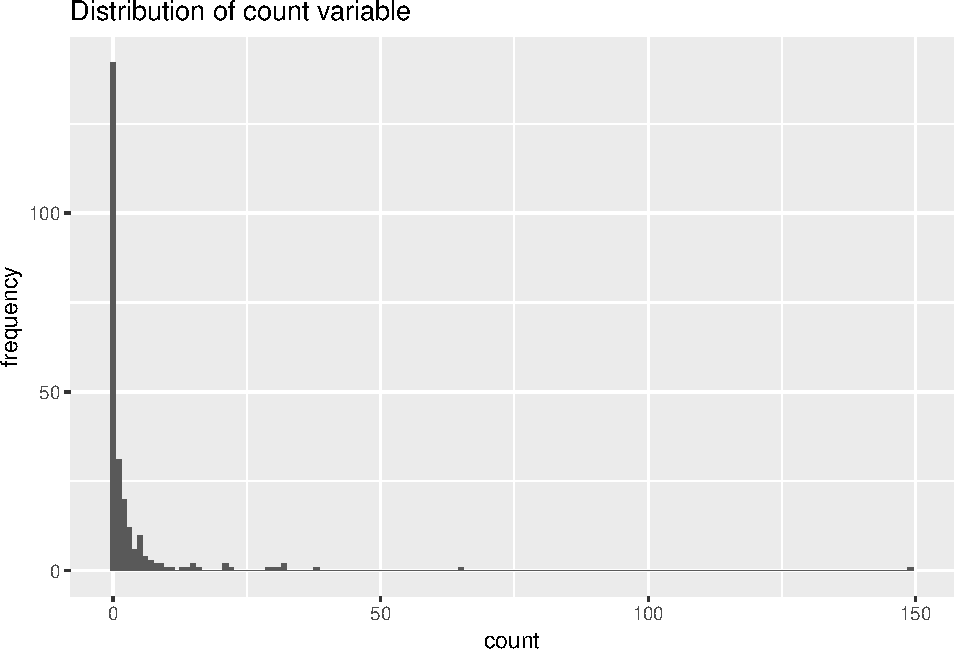
\includegraphics{05-poisreg_files/figure-latex/hist-1.pdf}

Предположим, что переменная имеет распределение Пуассона. Будем использовать пуассоновскую регрессию.
\[
P(y=k)=exp(-\lambda) \lambda^k / k!
\]
где \(\lambda=\exp(b_1 +b_2*x)\)

\begin{Shaded}
\begin{Highlighting}[]
\NormalTok{poisson_model =}\StringTok{ }\KeywordTok{glm}\NormalTok{(count }\OperatorTok{~}\StringTok{ }\NormalTok{child }\OperatorTok{+}\StringTok{ }\NormalTok{camper }\OperatorTok{+}\StringTok{  }\NormalTok{persons, }\DataTypeTok{family =} \StringTok{"poisson"}\NormalTok{, }\DataTypeTok{data =}\NormalTok{ df_fish)}
\KeywordTok{summary}\NormalTok{(poisson_model)}
\end{Highlighting}
\end{Shaded}

\begin{verbatim}

Call:
glm(formula = count ~ child + camper + persons, family = "poisson", 
    data = df_fish)

Deviance Residuals: 
    Min       1Q   Median       3Q      Max  
-6.8096  -1.4431  -0.9060  -0.0406  16.1417  

Coefficients:
            Estimate Std. Error z value Pr(>|z|)    
(Intercept) -1.98183    0.15226  -13.02   <2e-16 ***
child       -1.68996    0.08099  -20.87   <2e-16 ***
camper1      0.93094    0.08909   10.45   <2e-16 ***
persons      1.09126    0.03926   27.80   <2e-16 ***
---
Signif. codes:  0 '***' 0.001 '**' 0.01 '*' 0.05 '.' 0.1 ' ' 1

(Dispersion parameter for poisson family taken to be 1)

    Null deviance: 2958.4  on 249  degrees of freedom
Residual deviance: 1337.1  on 246  degrees of freedom
AIC: 1682.1

Number of Fisher Scoring iterations: 6
\end{verbatim}

Посчитаем средний предельный эффект для каждой переменной.

\begin{Shaded}
\begin{Highlighting}[]
\NormalTok{m =}\StringTok{ }\KeywordTok{margins}\NormalTok{(poisson_model)}
\end{Highlighting}
\end{Shaded}

\begin{verbatim}
Error in margins(poisson_model): could not find function "margins"
\end{verbatim}

\begin{Shaded}
\begin{Highlighting}[]
\KeywordTok{summary}\NormalTok{(m)}
\end{Highlighting}
\end{Shaded}

\begin{verbatim}
Error in summary(m): object 'm' not found
\end{verbatim}

\begin{Shaded}
\begin{Highlighting}[]
\KeywordTok{cplot}\NormalTok{(poisson_model, }\DataTypeTok{x =} \StringTok{'persons'}\NormalTok{, }\DataTypeTok{what =} \StringTok{'effect'}\NormalTok{, }\DataTypeTok{title =} \StringTok{'Предельный эффект переменной camper'}\NormalTok{)}
\end{Highlighting}
\end{Shaded}

\begin{verbatim}
Error in cplot(poisson_model, x = "persons", what = "effect", title = "Предельный эффект переменной camper"): could not find function "cplot"
\end{verbatim}

\begin{Shaded}
\begin{Highlighting}[]
\KeywordTok{margins}\NormalTok{(poisson_model, }\DataTypeTok{at =} \KeywordTok{list}\NormalTok{(}\DataTypeTok{child =} \DecValTok{0}\OperatorTok{:}\DecValTok{1}\NormalTok{)) }\CommentTok{# или в какой-нибудь точке}
\end{Highlighting}
\end{Shaded}

\begin{verbatim}
Error in margins(poisson_model, at = list(child = 0:1)): could not find function "margins"
\end{verbatim}

\begin{Shaded}
\begin{Highlighting}[]
\KeywordTok{plot_model}\NormalTok{(poisson_model, }\DataTypeTok{type =} \StringTok{'pred'}\NormalTok{)}
\end{Highlighting}
\end{Shaded}

\begin{verbatim}
$child
\end{verbatim}

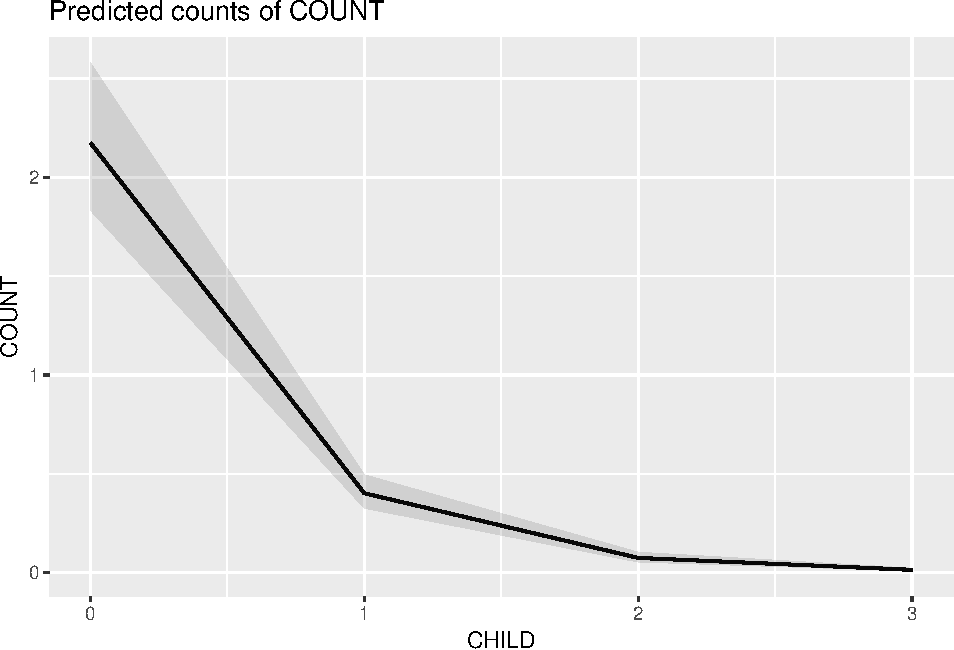
\includegraphics{05-poisreg_files/figure-latex/mef-1.pdf}

\begin{verbatim}

$camper
\end{verbatim}

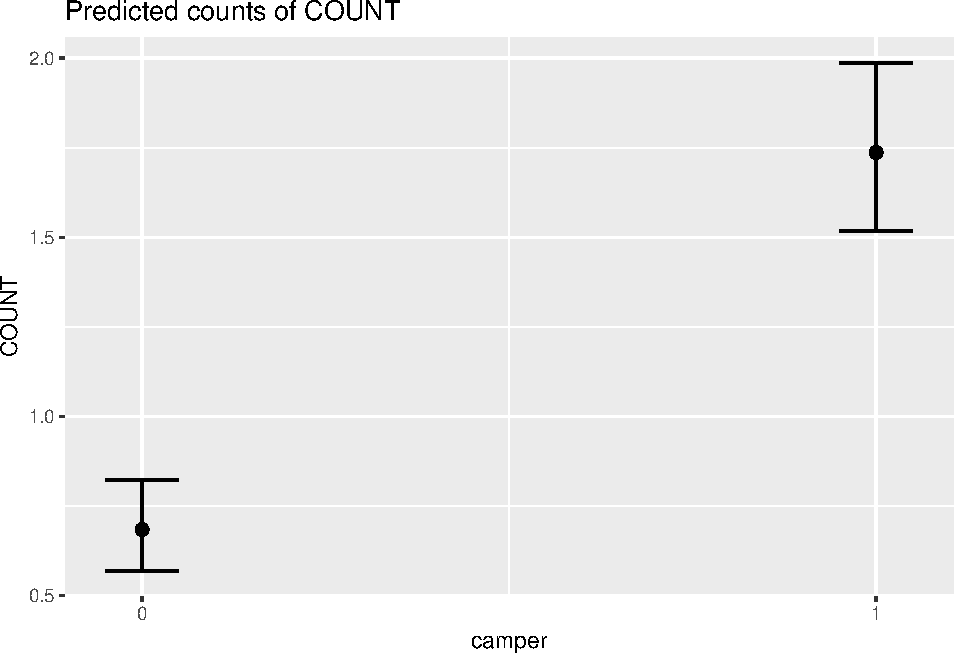
\includegraphics{05-poisreg_files/figure-latex/mef-2.pdf}

\begin{verbatim}

$persons
\end{verbatim}

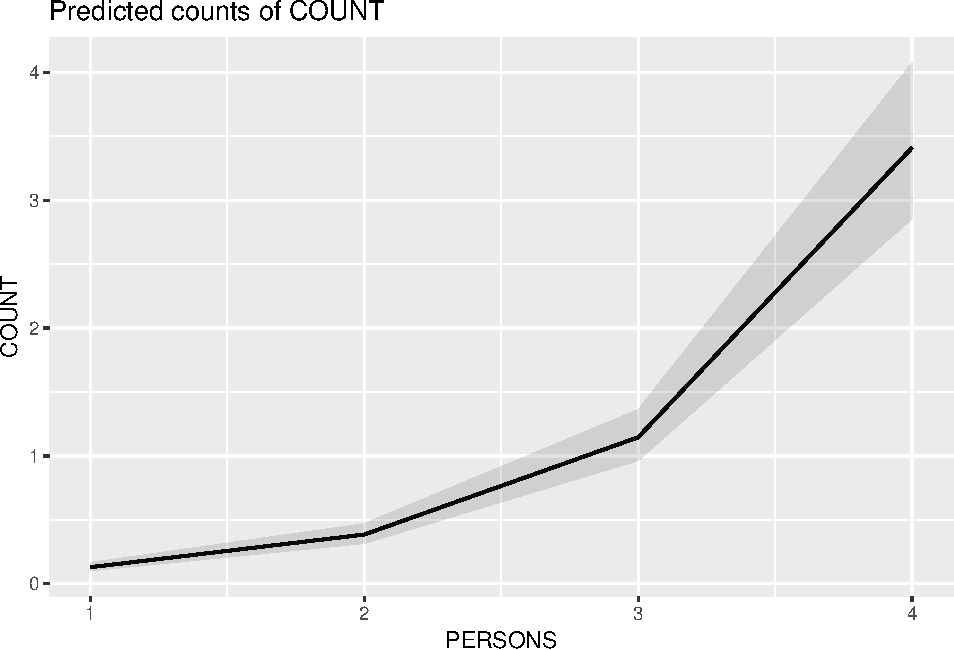
\includegraphics{05-poisreg_files/figure-latex/mef-3.pdf}

\begin{Shaded}
\begin{Highlighting}[]
\KeywordTok{plot_model}\NormalTok{(poisson_model, }\DataTypeTok{type =} \StringTok{"pred"}\NormalTok{, }\DataTypeTok{terms =} \KeywordTok{c}\NormalTok{(}\StringTok{"child [0, 0, 1]"}\NormalTok{, }\StringTok{"persons [1,3]"}\NormalTok{))}
\end{Highlighting}
\end{Shaded}

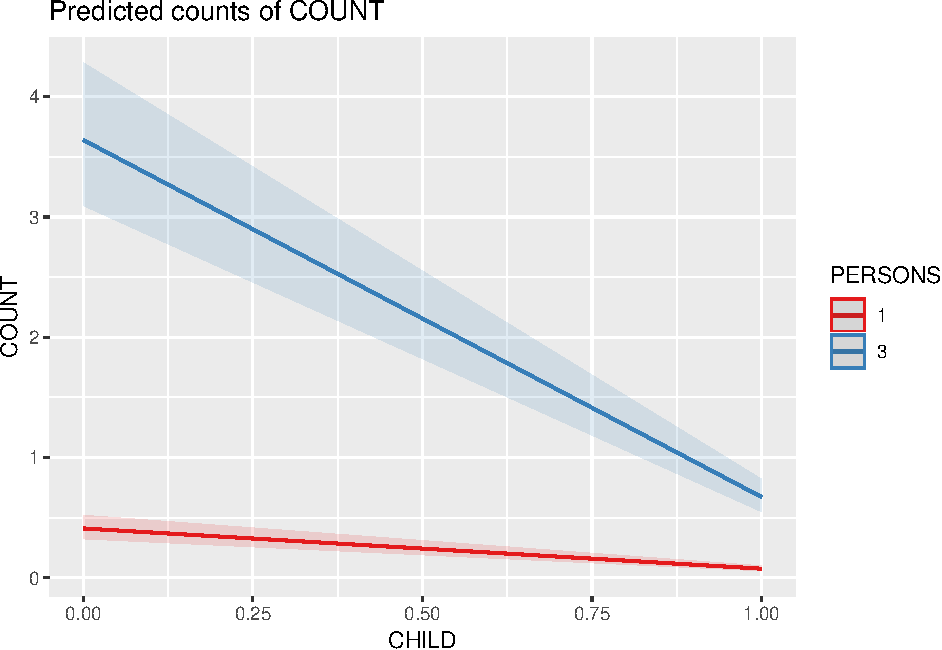
\includegraphics{05-poisreg_files/figure-latex/mef-4.pdf}

Однако, заметим, что дисперсия и среднее значение объясняемой переменной не равны, как это предполагает распределение Пуассона.

\begin{Shaded}
\begin{Highlighting}[]
\NormalTok{df_fish }\OperatorTok\StringTok{ }
\StringTok{  }\KeywordTok{group_by}\NormalTok{(camper) }\OperatorTok\StringTok{ }
\StringTok{  }\KeywordTok{summarize}\NormalTok{(}\DataTypeTok{var =} \KeywordTok{var}\NormalTok{(count), }\DataTypeTok{mean =} \KeywordTok{mean}\NormalTok{(count))}
\end{Highlighting}
\end{Shaded}

\begin{verbatim}
# A tibble: 2 x 3
  camper   var  mean
  <fct>  <dbl> <dbl>
1 0       21.1  1.52
2 1      212.   4.54
\end{verbatim}

Оценим регрессию, предполагая отрицательное биномиальное распределение остатков. В этом случае, дисперсия распределения зависит от некоторого параметра и не равна среднему.

\begin{Shaded}
\begin{Highlighting}[]
\NormalTok{nb1 =}\StringTok{ }\KeywordTok{glm.nb}\NormalTok{(count }\OperatorTok{~}\StringTok{ }\NormalTok{child }\OperatorTok{+}\StringTok{ }\NormalTok{camper }\OperatorTok{+}\StringTok{  }\NormalTok{persons, }\DataTypeTok{data =}\NormalTok{ df_fish)}
\KeywordTok{summary}\NormalTok{(nb1)}
\end{Highlighting}
\end{Shaded}

\begin{verbatim}

Call:
glm.nb(formula = count ~ child + camper + persons, data = df_fish, 
    init.theta = 0.4635287626, link = log)

Deviance Residuals: 
    Min       1Q   Median       3Q      Max  
-1.6673  -0.9599  -0.6590  -0.0319   4.9433  

Coefficients:
            Estimate Std. Error z value Pr(>|z|)    
(Intercept)  -1.6250     0.3304  -4.918 8.74e-07 ***
child        -1.7805     0.1850  -9.623  < 2e-16 ***
camper1       0.6211     0.2348   2.645  0.00816 ** 
persons       1.0608     0.1144   9.273  < 2e-16 ***
---
Signif. codes:  0 '***' 0.001 '**' 0.01 '*' 0.05 '.' 0.1 ' ' 1

(Dispersion parameter for Negative Binomial(0.4635) family taken to be 1)

    Null deviance: 394.25  on 249  degrees of freedom
Residual deviance: 210.65  on 246  degrees of freedom
AIC: 820.44

Number of Fisher Scoring iterations: 1

              Theta:  0.4635 
          Std. Err.:  0.0712 

 2 x log-likelihood:  -810.4440 
\end{verbatim}

Попробуем исключить из модели переменную \texttt{camper} и сравним качество двух моделей.

\begin{Shaded}
\begin{Highlighting}[]
\NormalTok{nb2 =}\StringTok{ }\KeywordTok{update}\NormalTok{(nb1, . }\OperatorTok{~}\StringTok{ }\NormalTok{. }\OperatorTok{-}\StringTok{ }\NormalTok{camper)}
\KeywordTok{waldtest}\NormalTok{(nb1, nb2)}
\end{Highlighting}
\end{Shaded}

\begin{verbatim}
Wald test

Model 1: count ~ child + camper + persons
Model 2: count ~ child + persons
  Res.Df Df      F   Pr(>F)   
1    246                      
2    247 -1 6.9979 0.008686 **
---
Signif. codes:  0 '***' 0.001 '**' 0.01 '*' 0.05 '.' 0.1 ' ' 1
\end{verbatim}

Можем посмотреть на результаты модели с ``раздутыми нулями'' (zero-inflated). Они предполагают большую частоту нулевых наблюдений.

\begin{Shaded}
\begin{Highlighting}[]
\NormalTok{zero_infl =}\StringTok{ }\KeywordTok{zeroinfl}\NormalTok{(count }\OperatorTok{~}\StringTok{  }\NormalTok{child }\OperatorTok{+}\StringTok{ }\NormalTok{camper }\OperatorTok{|}\StringTok{ }\NormalTok{persons, }\DataTypeTok{data =}\NormalTok{ df_fish, }\DataTypeTok{dist =} \StringTok{'negbin'}\NormalTok{)}
\end{Highlighting}
\end{Shaded}

\begin{verbatim}
Error in zeroinfl(count ~ child + camper | persons, data = df_fish, dist = "negbin"): could not find function "zeroinfl"
\end{verbatim}

\begin{Shaded}
\begin{Highlighting}[]
\KeywordTok{summary}\NormalTok{(zero_infl)}
\end{Highlighting}
\end{Shaded}

\begin{verbatim}
Error in summary(zero_infl): object 'zero_infl' not found
\end{verbatim}

\begin{Shaded}
\begin{Highlighting}[]
\KeywordTok{plot_model}\NormalTok{(zero_infl, }\DataTypeTok{type =} \StringTok{'pred'}\NormalTok{)}
\end{Highlighting}
\end{Shaded}

\begin{verbatim}
Error in insight::model_info(model): object 'zero_infl' not found
\end{verbatim}

\hypertarget{python-1}{%
\section{python}\label{python-1}}

Нужные пакетики:

\begin{Shaded}
\begin{Highlighting}[]
\ImportTok{import}\NormalTok{ pandas }\ImportTok{as}\NormalTok{ pd }\CommentTok{# для работы с таблицами}
\end{Highlighting}
\end{Shaded}

\begin{verbatim}
Error in py_call_impl(callable, dots$args, dots$keywords): ModuleNotFoundError: No module named 'pandas'

Detailed traceback: 
  File "<string>", line 1, in <module>
\end{verbatim}

\begin{Shaded}
\begin{Highlighting}[]
\ImportTok{import}\NormalTok{ numpy }\ImportTok{as}\NormalTok{ np }\CommentTok{# математика, работа с матрицами}
\ImportTok{import}\NormalTok{ matplotlib.pyplot }\ImportTok{as}\NormalTok{ plt }\CommentTok{# графики}
\end{Highlighting}
\end{Shaded}

\begin{verbatim}
Error in py_call_impl(callable, dots$args, dots$keywords): ModuleNotFoundError: No module named 'matplotlib'

Detailed traceback: 
  File "<string>", line 1, in <module>
\end{verbatim}

\begin{Shaded}
\begin{Highlighting}[]
\ImportTok{import}\NormalTok{ statsmodels.api }\ImportTok{as}\NormalTok{ sm}
\end{Highlighting}
\end{Shaded}

\begin{verbatim}
Error in py_call_impl(callable, dots$args, dots$keywords): ModuleNotFoundError: No module named 'statsmodels'

Detailed traceback: 
  File "<string>", line 1, in <module>
\end{verbatim}

\begin{Shaded}
\begin{Highlighting}[]
\ImportTok{import}\NormalTok{ statsmodels.formula.api }\ImportTok{as}\NormalTok{ smf}
\end{Highlighting}
\end{Shaded}

\begin{verbatim}
Error in py_call_impl(callable, dots$args, dots$keywords): ModuleNotFoundError: No module named 'statsmodels'

Detailed traceback: 
  File "<string>", line 1, in <module>
\end{verbatim}

\begin{Shaded}
\begin{Highlighting}[]
\ImportTok{import}\NormalTok{ statsmodels.graphics.gofplots }\ImportTok{as}\NormalTok{ gf}
\end{Highlighting}
\end{Shaded}

\begin{verbatim}
Error in py_call_impl(callable, dots$args, dots$keywords): ModuleNotFoundError: No module named 'statsmodels'

Detailed traceback: 
  File "<string>", line 1, in <module>
\end{verbatim}

\begin{Shaded}
\begin{Highlighting}[]
\ImportTok{from}\NormalTok{ statsmodels.stats.outliers_influence }\ImportTok{import}\NormalTok{ summary_table}
\end{Highlighting}
\end{Shaded}

\begin{verbatim}
Error in py_call_impl(callable, dots$args, dots$keywords): ModuleNotFoundError: No module named 'statsmodels'

Detailed traceback: 
  File "<string>", line 1, in <module>
\end{verbatim}

\begin{Shaded}
\begin{Highlighting}[]
\ImportTok{import}\NormalTok{ seaborn }\ImportTok{as}\NormalTok{ sns }\CommentTok{# еще более классные графики}
\end{Highlighting}
\end{Shaded}

\begin{verbatim}
Error in py_call_impl(callable, dots$args, dots$keywords): ModuleNotFoundError: No module named 'seaborn'

Detailed traceback: 
  File "<string>", line 1, in <module>
\end{verbatim}

\begin{Shaded}
\begin{Highlighting}[]
\ImportTok{from}\NormalTok{ scipy.stats }\ImportTok{import}\NormalTok{ shapiro }\CommentTok{# еще математика}
\end{Highlighting}
\end{Shaded}

\begin{verbatim}
Error in py_call_impl(callable, dots$args, dots$keywords): ModuleNotFoundError: No module named 'scipy'

Detailed traceback: 
  File "<string>", line 1, in <module>
\end{verbatim}

\begin{Shaded}
\begin{Highlighting}[]
\ImportTok{import}\NormalTok{ statsmodels.discrete.discrete_model}
\end{Highlighting}
\end{Shaded}

\begin{verbatim}
Error in py_call_impl(callable, dots$args, dots$keywords): ModuleNotFoundError: No module named 'statsmodels'

Detailed traceback: 
  File "<string>", line 1, in <module>
\end{verbatim}

\begin{Shaded}
\begin{Highlighting}[]
\ImportTok{from}\NormalTok{ statsmodels.discrete.count_model }\ImportTok{import}\NormalTok{ ZeroInflatedPoisson}
\end{Highlighting}
\end{Shaded}

\begin{verbatim}
Error in py_call_impl(callable, dots$args, dots$keywords): ModuleNotFoundError: No module named 'statsmodels'

Detailed traceback: 
  File "<string>", line 1, in <module>
\end{verbatim}

\begin{Shaded}
\begin{Highlighting}[]
\NormalTok{plt.style.use(}\StringTok{'ggplot'}\NormalTok{)}
\end{Highlighting}
\end{Shaded}

\begin{verbatim}
Error in py_call_impl(callable, dots$args, dots$keywords): NameError: name 'plt' is not defined

Detailed traceback: 
  File "<string>", line 1, in <module>
\end{verbatim}

Загружаем данные и смотрим описательные статистики.

\begin{Shaded}
\begin{Highlighting}[]
\NormalTok{df_fish }\OperatorTok{=}\NormalTok{ pd.read_stata(}\StringTok{'data/fish.dta'}\NormalTok{)}
\end{Highlighting}
\end{Shaded}

\begin{verbatim}
Error in py_call_impl(callable, dots$args, dots$keywords): NameError: name 'pd' is not defined

Detailed traceback: 
  File "<string>", line 1, in <module>
\end{verbatim}

\begin{Shaded}
\begin{Highlighting}[]
\NormalTok{sns.distplot(df_fish[}\StringTok{'count'}\NormalTok{])}
\end{Highlighting}
\end{Shaded}

\begin{verbatim}
Error in py_call_impl(callable, dots$args, dots$keywords): NameError: name 'sns' is not defined

Detailed traceback: 
  File "<string>", line 1, in <module>
\end{verbatim}

\begin{Shaded}
\begin{Highlighting}[]
\NormalTok{plt.show()}
\end{Highlighting}
\end{Shaded}

\begin{verbatim}
Error in py_call_impl(callable, dots$args, dots$keywords): NameError: name 'plt' is not defined

Detailed traceback: 
  File "<string>", line 1, in <module>
\end{verbatim}

Превращаем переменную \texttt{camper} в категориальную.

\begin{Shaded}
\begin{Highlighting}[]
\NormalTok{df_fish[}\StringTok{'camper'}\NormalTok{] }\OperatorTok{=}\NormalTok{ df_fish[}\StringTok{'camper'}\NormalTok{].astype(}\StringTok{'category'}\NormalTok{)}
\end{Highlighting}
\end{Shaded}

\begin{verbatim}
Error in py_call_impl(callable, dots$args, dots$keywords): NameError: name 'df_fish' is not defined

Detailed traceback: 
  File "<string>", line 1, in <module>
\end{verbatim}

Строим Пуассоновскую регрессию.

\begin{Shaded}
\begin{Highlighting}[]
\NormalTok{pois }\OperatorTok{=}\NormalTok{ statsmodels.discrete.discrete_model.Poisson(endog }\OperatorTok{=}\NormalTok{ count, exog }\OperatorTok{=}\NormalTok{ np.array(child, camper, persons), data}\OperatorTok{=}\NormalTok{df_fish)}
\end{Highlighting}
\end{Shaded}

\begin{verbatim}
Error in py_call_impl(callable, dots$args, dots$keywords): NameError: name 'statsmodels' is not defined

Detailed traceback: 
  File "<string>", line 1, in <module>
\end{verbatim}

\begin{Shaded}
\begin{Highlighting}[]
\NormalTok{regr_pois }\OperatorTok{=}\NormalTok{ smf.glm(}\StringTok{'count ~ child + camper +  persons'}\NormalTok{, data}\OperatorTok{=}\NormalTok{df_fish,}
\NormalTok{                    family}\OperatorTok{=}\NormalTok{sm.families.Poisson()).fit()}
\end{Highlighting}
\end{Shaded}

\begin{verbatim}
Error in py_call_impl(callable, dots$args, dots$keywords): NameError: name 'smf' is not defined

Detailed traceback: 
  File "<string>", line 1, in <module>
\end{verbatim}

\begin{Shaded}
\begin{Highlighting}[]
\NormalTok{regr_pois.summary()}
\end{Highlighting}
\end{Shaded}

\begin{verbatim}
Error in py_call_impl(callable, dots$args, dots$keywords): NameError: name 'regr_pois' is not defined

Detailed traceback: 
  File "<string>", line 1, in <module>
\end{verbatim}

Посмотрим, равны ли среднее значение и дисперсия, как это предполагает распределение Пуассона.

\begin{Shaded}
\begin{Highlighting}[]
\NormalTok{(df_fish}
\NormalTok{ .}\BuiltInTok{filter}\NormalTok{([}\StringTok{'count'}\NormalTok{, }\StringTok{'camper'}\NormalTok{])}
\NormalTok{ .groupby(}\StringTok{'camper'}\NormalTok{)}
\NormalTok{ .agg([}\StringTok{'mean'}\NormalTok{, }\StringTok{'var'}\NormalTok{]))}
\end{Highlighting}
\end{Shaded}

\begin{verbatim}
Error in py_call_impl(callable, dots$args, dots$keywords): NameError: name 'df_fish' is not defined

Detailed traceback: 
  File "<string>", line 1, in <module>
\end{verbatim}

И регрессию с остатками, имеющими отрицательное биномиальное распределение.

\begin{Shaded}
\begin{Highlighting}[]
\NormalTok{regr_bin }\OperatorTok{=}\NormalTok{ smf.glm(}\StringTok{'count ~ child + camper +  persons'}\NormalTok{, data}\OperatorTok{=}\NormalTok{df_fish,}
\NormalTok{              family}\OperatorTok{=}\NormalTok{sm.families.NegativeBinomial()).fit()}
\end{Highlighting}
\end{Shaded}

\begin{verbatim}
Error in py_call_impl(callable, dots$args, dots$keywords): NameError: name 'smf' is not defined

Detailed traceback: 
  File "<string>", line 1, in <module>
\end{verbatim}

\begin{Shaded}
\begin{Highlighting}[]
\NormalTok{regr_bin.summary()}
\end{Highlighting}
\end{Shaded}

\begin{verbatim}
Error in py_call_impl(callable, dots$args, dots$keywords): NameError: name 'regr_bin' is not defined

Detailed traceback: 
  File "<string>", line 1, in <module>
\end{verbatim}

Проверим гипотезу о равенстве 0 коэффициента при переменной \texttt{camper}. Проведем тест Вальда.

\begin{Shaded}
\begin{Highlighting}[]
\NormalTok{hyp }\OperatorTok{=} \StringTok{'(child = 0)'}
\NormalTok{regr_bin.wald_test(hyp)}
\end{Highlighting}
\end{Shaded}

\begin{verbatim}
Error in py_call_impl(callable, dots$args, dots$keywords): NameError: name 'regr_bin' is not defined

Detailed traceback: 
  File "<string>", line 1, in <module>
\end{verbatim}

Посчитаем средний предельный эффект для каждой переменной.

\begin{Shaded}
\begin{Highlighting}[]
\NormalTok{pred }\OperatorTok{=}\NormalTok{ regr_pois.fittedvalues}
\end{Highlighting}
\end{Shaded}

\begin{verbatim}
Error in py_call_impl(callable, dots$args, dots$keywords): NameError: name 'regr_pois' is not defined

Detailed traceback: 
  File "<string>", line 1, in <module>
\end{verbatim}

\begin{Shaded}
\begin{Highlighting}[]
\NormalTok{mean_mef_child }\OperatorTok{=}\NormalTok{ np.mean([regr_pois.params[}\DecValTok{1}\NormalTok{] }\OperatorTok{*}\NormalTok{ p }\ControlFlowTok{for}\NormalTok{ p }\KeywordTok{in}\NormalTok{ pred])}
\end{Highlighting}
\end{Shaded}

\begin{verbatim}
Error in py_call_impl(callable, dots$args, dots$keywords): NameError: name 'pred' is not defined

Detailed traceback: 
  File "<string>", line 1, in <module>
\end{verbatim}

\begin{Shaded}
\begin{Highlighting}[]
\NormalTok{mean_mef_camper }\OperatorTok{=}\NormalTok{ np.mean([regr_pois.params[}\DecValTok{2}\NormalTok{] }\OperatorTok{*}\NormalTok{ p }\ControlFlowTok{for}\NormalTok{ p }\KeywordTok{in}\NormalTok{ pred])}
\end{Highlighting}
\end{Shaded}

\begin{verbatim}
Error in py_call_impl(callable, dots$args, dots$keywords): NameError: name 'pred' is not defined

Detailed traceback: 
  File "<string>", line 1, in <module>
\end{verbatim}

\begin{Shaded}
\begin{Highlighting}[]
\NormalTok{data_1 }\OperatorTok{=}\NormalTok{ pd.DataFrame(\{}\StringTok{'child'}\NormalTok{: df_fish[}\StringTok{'child'}\NormalTok{], }\StringTok{'camper'}\NormalTok{: }\DecValTok{1}\NormalTok{, }\StringTok{'persons'}\NormalTok{: df_fish[}\StringTok{'persons'}\NormalTok{]\})}
\end{Highlighting}
\end{Shaded}

\begin{verbatim}
Error in py_call_impl(callable, dots$args, dots$keywords): NameError: name 'pd' is not defined

Detailed traceback: 
  File "<string>", line 1, in <module>
\end{verbatim}

\begin{Shaded}
\begin{Highlighting}[]
\NormalTok{data_0 }\OperatorTok{=}\NormalTok{ pd.DataFrame(\{}\StringTok{'child'}\NormalTok{: df_fish[}\StringTok{'child'}\NormalTok{], }\StringTok{'camper'}\NormalTok{: }\DecValTok{0}\NormalTok{, }\StringTok{'persons'}\NormalTok{: df_fish[}\StringTok{'persons'}\NormalTok{]\})}
\end{Highlighting}
\end{Shaded}

\begin{verbatim}
Error in py_call_impl(callable, dots$args, dots$keywords): NameError: name 'pd' is not defined

Detailed traceback: 
  File "<string>", line 1, in <module>
\end{verbatim}

\begin{Shaded}
\begin{Highlighting}[]
\NormalTok{mean_mef_persons }\OperatorTok{=}\NormalTok{ np.mean([(regr_pois.predict(data_1)[i]}\OperatorTok{-}\NormalTok{regr_pois.predict(data_0)[i]) }
                            \ControlFlowTok{for}\NormalTok{ i }\KeywordTok{in} \BuiltInTok{range}\NormalTok{(}\BuiltInTok{len}\NormalTok{(df_fish))])}
\end{Highlighting}
\end{Shaded}

\begin{verbatim}
Error in py_call_impl(callable, dots$args, dots$keywords): NameError: name 'df_fish' is not defined

Detailed traceback: 
  File "<string>", line 2, in <module>
\end{verbatim}

\begin{Shaded}
\begin{Highlighting}[]
\NormalTok{plot_model(regr_pois, }\BuiltInTok{type} \OperatorTok{=} \StringTok{'effect'}\NormalTok{, terms }\OperatorTok{=} \StringTok{'camper'}\NormalTok{)}
\end{Highlighting}
\end{Shaded}

\begin{verbatim}
Error in py_call_impl(callable, dots$args, dots$keywords): NameError: name 'plot_model' is not defined

Detailed traceback: 
  File "<string>", line 1, in <module>
\end{verbatim}

И модель с раздутыми нулями. (которой нет)

\hypertarget{stata-1}{%
\section{stata}\label{stata-1}}

Загружаем данные и смотрим описательные статистики.

\begin{verbatim}
use data/fish.dta
summarize
\end{verbatim}

\begin{verbatim}
    Variable |        Obs        Mean    Std. Dev.       Min        Max
-------------+---------------------------------------------------------
      camper |        250        .588    .4931824          0          1
       child |        250        .684    .8503153          0          3
       count |        250       3.296    11.63503          0        149
     persons |        250       2.528     1.11273          1          4
\end{verbatim}

\begin{verbatim}
hist count
\end{verbatim}

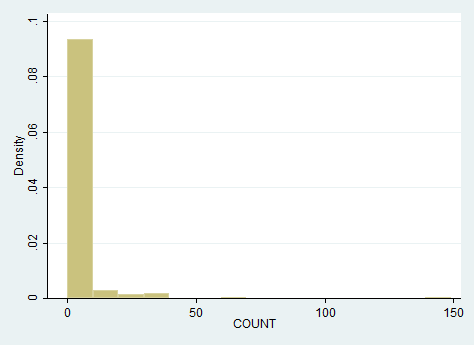
\includegraphics{hist_pois.png}

Строим Пуассоновскую регрессию.
В описательных статистиках:
\(AIC = -2log(L) + 2k\)
\(AIC = -2log(L) + klog(N)\)

\begin{verbatim}
glm count camper child persons, family(poisson)
\end{verbatim}

\begin{verbatim}
 translator Graph2png not found
r(111);



Iteration 0:   log likelihood = -965.92815  
Iteration 1:   log likelihood = -837.97093  
Iteration 2:   log likelihood = -837.07307  
Iteration 3:   log likelihood = -837.07248  
Iteration 4:   log likelihood = -837.07248  

Generalized linear models                         No. of obs      =        250
Optimization     : ML                             Residual df     =        246
                                                  Scale parameter =          1
Deviance         =  1337.079644                   (1/df) Deviance =   5.435283
Pearson          =  2910.627049                   (1/df) Pearson  =   11.83182

Variance function: V(u) = u                       [Poisson]
Link function    : g(u) = ln(u)                   [Log]

                                                  AIC             =    6.72858
Log likelihood   = -837.0724803                   BIC             =  -21.19974

------------------------------------------------------------------------------
             |                 OIM
       count |      Coef.   Std. Err.      z    P>|z|     [95% Conf. Interval]
-------------+----------------------------------------------------------------
      camper |   .9309359   .0890869    10.45   0.000     .7563289    1.105543
       child |  -1.689957   .0809922   -20.87   0.000    -1.848699   -1.531215
     persons |   1.091262   .0392553    27.80   0.000     1.014323    1.168201
       _cons |  -1.981827    .152263   -13.02   0.000    -2.280257   -1.683397
------------------------------------------------------------------------------
\end{verbatim}

Можем посчитать AIC и BIC по другой формуле, аналогично выводу R.
\(AIC = \frac {-2log(L) + 2k}{N}\)

\begin{verbatim}
estat ic
\end{verbatim}

\begin{verbatim}
 translator Graph2png not found
r(111);


last estimates not found
r(301);

end of do-file
r(301);
\end{verbatim}

Посмотрим, равны ли среднее значение и дисперсия, как это предполагает распределение Пуассона.

\begin{verbatim}
tabstat count, by(camper) stat(mean, variance) nototal
\end{verbatim}

\begin{verbatim}
 translator Graph2png not found
r(111);



Summary for variables: count
     by categories of: camper (CAMPER)

  camper |      mean  variance
---------+--------------------
       0 |  1.524272  21.05578
       1 |  4.537415   212.401
------------------------------
\end{verbatim}

Предположим, что остатки имеют отрицательное биномиальное распределение.

\begin{verbatim}
nbreg count child camper persons
\end{verbatim}

\begin{verbatim}
 translator Graph2png not found
r(111);



Fitting Poisson model:

Iteration 0:   log likelihood = -841.58831  
Iteration 1:   log likelihood = -837.07386  
Iteration 2:   log likelihood = -837.07248  
Iteration 3:   log likelihood = -837.07248  

Fitting constant-only model:

Iteration 0:   log likelihood = -582.76028  
Iteration 1:   log likelihood = -464.44518  
Iteration 2:   log likelihood = -464.43931  
Iteration 3:   log likelihood = -464.43931  

Fitting full model:

Iteration 0:   log likelihood = -438.02759  
Iteration 1:   log likelihood = -409.71171  
Iteration 2:   log likelihood = -405.34765  
Iteration 3:   log likelihood = -405.22204  
Iteration 4:   log likelihood =   -405.222  
Iteration 5:   log likelihood =   -405.222  

Negative binomial regression                    Number of obs     =        250
                                                LR chi2(3)        =     118.43
Dispersion     = mean                           Prob > chi2       =     0.0000
Log likelihood =   -405.222                     Pseudo R2         =     0.1275

------------------------------------------------------------------------------
       count |      Coef.   Std. Err.      z    P>|z|     [95% Conf. Interval]
-------------+----------------------------------------------------------------
       child |   -1.78052   .1920379    -9.27   0.000    -2.156907   -1.404132
      camper |   .6211286   .2358072     2.63   0.008      .158955    1.083302
     persons |     1.0608   .1174733     9.03   0.000     .8305564    1.291043
       _cons |   -1.62499   .3294006    -4.93   0.000    -2.270603   -.9793765
-------------+----------------------------------------------------------------
    /lnalpha |   .7688868   .1538497                      .4673469    1.070427
-------------+----------------------------------------------------------------
       alpha |   2.157363   .3319098                      1.595755    2.916624
------------------------------------------------------------------------------
LR test of alpha=0: chibar2(01) = 863.70               Prob >= chibar2 = 0.000
\end{verbatim}

Проверим гипотезу о равенстве 0 коэффицинта при переменной \texttt{camper}. Проведем тест Вальда.

\begin{verbatim}
quietly: nbreg count child i.camper persons 
test i.camper 
\end{verbatim}

\begin{verbatim}
 translator Graph2png not found
r(111);



i:  operator invalid
r(198);

end of do-file
r(198);
\end{verbatim}

Посчитаем средний предельный эффект для каждой переменной.

\begin{verbatim}
margins, dydx(*)
marginsplot
\end{verbatim}

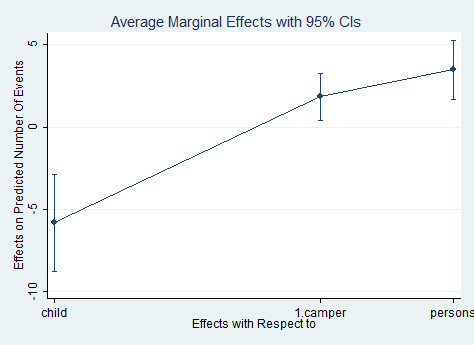
\includegraphics{margins_plot.png}

И модель с раздутыми нулями.

\begin{verbatim}
zinb count child i.camper, inflate(persons)
\end{verbatim}

\begin{verbatim}
 translator Graph2png not found
r(111);



Fitting constant-only model:

Iteration 0:   log likelihood = -519.33992  
Iteration 1:   log likelihood = -471.96077  
Iteration 2:   log likelihood = -465.38193  
Iteration 3:   log likelihood = -464.39882  
Iteration 4:   log likelihood = -463.92704  
Iteration 5:   log likelihood = -463.79248  
Iteration 6:   log likelihood = -463.75773  
Iteration 7:   log likelihood =  -463.7518  
Iteration 8:   log likelihood = -463.75119  
Iteration 9:   log likelihood = -463.75118  

Fitting full model:

Iteration 0:   log likelihood = -463.75118  (not concave)
Iteration 1:   log likelihood = -440.43162  
Iteration 2:   log likelihood = -434.96651  
Iteration 3:   log likelihood = -433.49903  
Iteration 4:   log likelihood = -432.89949  
Iteration 5:   log likelihood = -432.89091  
Iteration 6:   log likelihood = -432.89091  

Zero-inflated negative binomial regression      Number of obs     =        250
                                                Nonzero obs       =        108
                                                Zero obs          =        142

Inflation model = logit                         LR chi2(2)        =      61.72
Log likelihood  = -432.8909                     Prob > chi2       =     0.0000

------------------------------------------------------------------------------
       count |      Coef.   Std. Err.      z    P>|z|     [95% Conf. Interval]
-------------+----------------------------------------------------------------
count        |
       child |  -1.515255   .1955912    -7.75   0.000    -1.898606   -1.131903
       _cons |   1.371048   .2561131     5.35   0.000     .8690758    1.873021
-------------+----------------------------------------------------------------
inflate      |
     persons |  -1.666563   .6792833    -2.45   0.014    -2.997934   -.3351922
       _cons |   1.603104   .8365065     1.92   0.055     -.036419    3.242626
-------------+----------------------------------------------------------------
    /lnalpha |   .9853533     .17595     5.60   0.000     .6404975    1.330209
-------------+----------------------------------------------------------------
       alpha |   2.678758   .4713275                      1.897425    3.781834
------------------------------------------------------------------------------
\end{verbatim}

\hypertarget{disordered}{%
\chapter{Модели неупорядоченного выбора}\label{disordered}}

\hypertarget{instruments}{%
\chapter{Интcтрументы для простой регрессии}\label{instruments}}

\hypertarget{arma}{%
\chapter{ARMA}\label{arma}}

\begin{quote}
Достигнем просветления в анализе временных рядов вместе с нашими друзьями, stata, r и python!
В качестве анализируемых наблюдений используем данные по стоимости акций коммапнии \texttt{Apple} c 2015 - 01 - 01 по 2015 - 12 - 31: цена открытия/ закрытия, минимальная/ максимальная цены, объём и скорректиованная цена.
\end{quote}

\hypertarget{r-2}{%
\section{r}\label{r-2}}

Традиционно начнём в \textbf{r}.

Загрузим необходимые пакеты:

\begin{Shaded}
\begin{Highlighting}[]
\KeywordTok{library}\NormalTok{(xts) }\CommentTok{# работа с временными рядами}
\KeywordTok{library}\NormalTok{(dplyr) }\CommentTok{# манипуляции с данными}
\KeywordTok{library}\NormalTok{(ggplot2) }\CommentTok{# построение графиков}
\KeywordTok{library}\NormalTok{(aTSA) }\CommentTok{# тест Дики-Фуллера}
\end{Highlighting}
\end{Shaded}

\begin{verbatim}
Error in library(aTSA): there is no package called 'aTSA'
\end{verbatim}

\begin{Shaded}
\begin{Highlighting}[]
\KeywordTok{library}\NormalTok{(forecast) }\CommentTok{# прогнозирование ARMA-моделей}
\KeywordTok{library}\NormalTok{(quantmod) }\CommentTok{# импортирование dataset}
\KeywordTok{library}\NormalTok{(lmtest) }\CommentTok{# проверка гипотез}
\end{Highlighting}
\end{Shaded}

Импортируем dataset \texttt{AAPL} прямо из пакета \texttt{quantmod}. Будем анализировать одномерный временной ряд от переменной \texttt{AAPL.\ Close}.

\begin{Shaded}
\begin{Highlighting}[]
\KeywordTok{getSymbols}\NormalTok{(}\StringTok{"AAPL"}\NormalTok{,}\DataTypeTok{from=}\StringTok{"2015-01-01"}\NormalTok{,}\DataTypeTok{to=}\StringTok{"2015-12-31"}\NormalTok{)}
\end{Highlighting}
\end{Shaded}

\begin{verbatim}
[1] "AAPL"
\end{verbatim}

Обозначим наш dataframe как \texttt{apple\_df}.

\begin{Shaded}
\begin{Highlighting}[]
\NormalTok{apple_df =}\StringTok{ }\NormalTok{AAPL}\OperatorTok{$}\NormalTok{AAPL.Close}
\end{Highlighting}
\end{Shaded}

Визуализируем исследуемый временной ряд, его автокорреляционную и частную автокорреляционную функции.

\begin{Shaded}
\begin{Highlighting}[]
\KeywordTok{ggtsdisplay}\NormalTok{(apple_df)}
\end{Highlighting}
\end{Shaded}

\begin{center}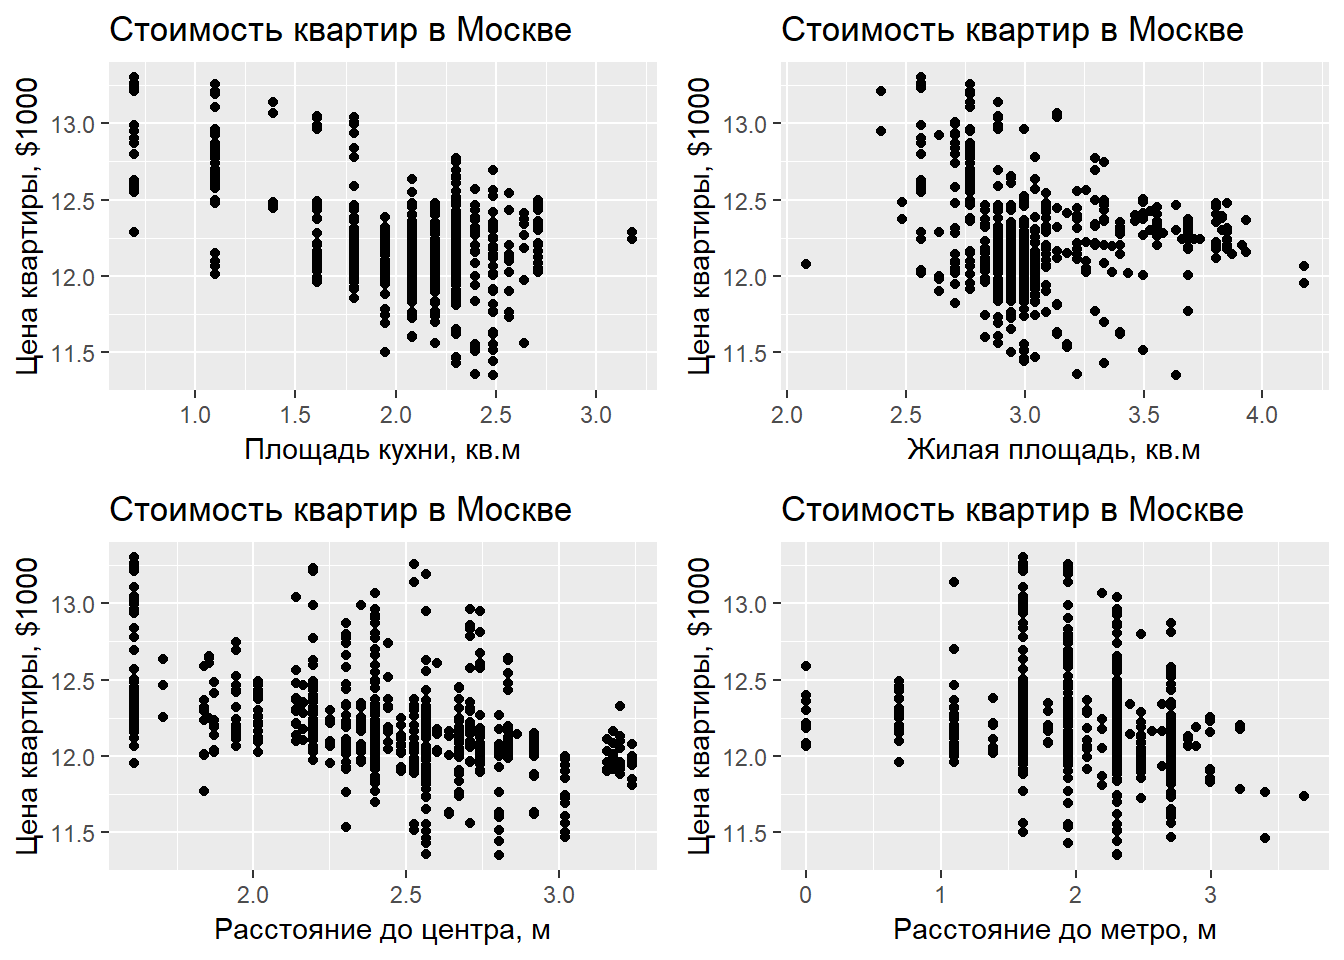
\includegraphics{08-arma_files/figure-latex/unnamed-chunk-5-1} \end{center}

По графику видим, что процесс напоминает случайное блуждание: медленно убывает автокорреляционная функция, первый лаг частной автокорреляционной функции не входит в доверительный интервал, остальные - входят.

Проверим стационарность ряда тестом Дики-Фуллера.

\begin{Shaded}
\begin{Highlighting}[]
\KeywordTok{adf.test}\NormalTok{(apple_df)}
\end{Highlighting}
\end{Shaded}

\begin{verbatim}
Error in adf.test(apple_df): could not find function "adf.test"
\end{verbatim}

Тест выявил нестационарность на 5\% уровне значимости (основная гипотеза -- о нестационарности ряда).

Возьмём первую разность от ряда, чтобы сделать его стационарным (ведь только стационарные процессы могут быть описаны моделью \texttt{ARMA\ (p,\ q)} ) и снова построим автокорреляционную и частную автокорреляционную функции.

\begin{Shaded}
\begin{Highlighting}[]
\NormalTok{apple_diff =}\StringTok{ }\KeywordTok{diff}\NormalTok{(apple_df)}
\KeywordTok{ggtsdisplay}\NormalTok{(apple_diff)}
\end{Highlighting}
\end{Shaded}

\begin{center}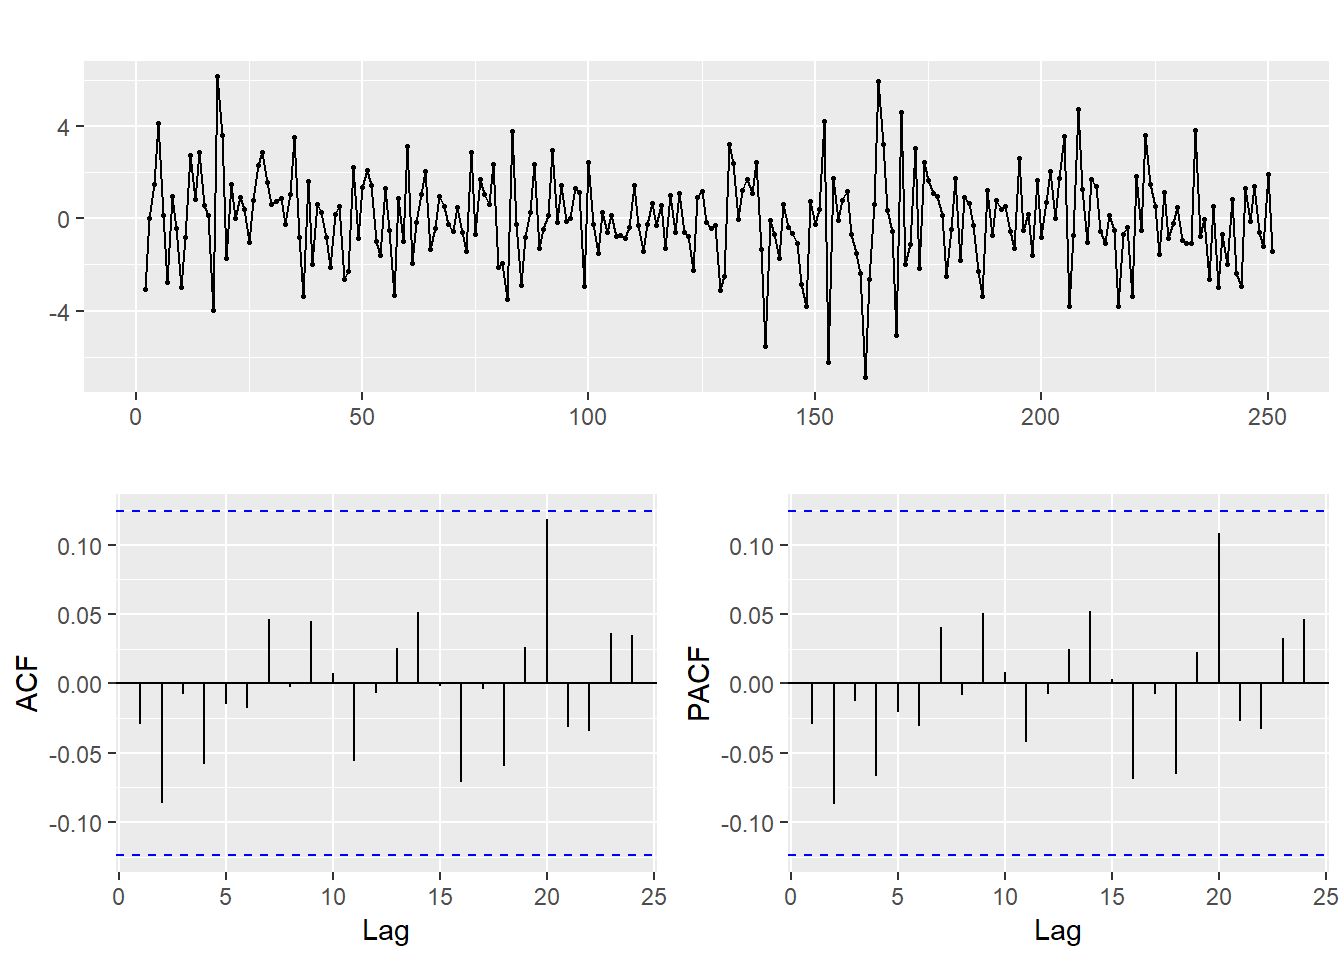
\includegraphics{08-arma_files/figure-latex/unnamed-chunk-7-1} \end{center}

\begin{Shaded}
\begin{Highlighting}[]
\KeywordTok{summary}\NormalTok{(apple_diff)}
\end{Highlighting}
\end{Shaded}

\begin{verbatim}
     Index              AAPL.Close      
 Min.   :2015-01-02   Min.   :-6.89000  
 1st Qu.:2015-04-04   1st Qu.:-1.02500  
 Median :2015-07-02   Median :-0.07500  
 Mean   :2015-07-02   Mean   :-0.00804  
 3rd Qu.:2015-09-30   3rd Qu.: 1.14499  
 Max.   :2015-12-30   Max.   : 6.17000  
                      NA's   :1         
\end{verbatim}

Ряд похож на стационарный. Теперь построим несколько моделей, которые потенциально могут описать данный ряд, хотя уже заранее ожидается, что ряд в разностях будет описан \texttt{ARIMA\ (0,\ 0,\ 0)}, что равносильно \texttt{ARMA(0,\ 0)}, но всё же\ldots{}

\texttt{ARIMA\ (0,\ 0,\ 0)}:

\begin{Shaded}
\begin{Highlighting}[]
\NormalTok{arima_}\DecValTok{000}\NormalTok{ =}\StringTok{ }\KeywordTok{arima}\NormalTok{(apple_diff, }\DataTypeTok{order=}\KeywordTok{c}\NormalTok{(}\DecValTok{0}\NormalTok{, }\DecValTok{0}\NormalTok{, }\DecValTok{0}\NormalTok{))}
\KeywordTok{summary}\NormalTok{(arima_}\DecValTok{000}\NormalTok{)}
\end{Highlighting}
\end{Shaded}

\begin{verbatim}

Call:
arima(x = apple_diff, order = c(0, 0, 0))

Coefficients:
      intercept
        -0.0080
s.e.     0.1244

sigma^2 estimated as 3.867:  log likelihood = -523.79,  aic = 1051.58

Training set error measures:
                       ME     RMSE      MAE      MPE     MAPE      MASE
Training set 8.078552e-15 1.966425 1.495158 99.55996 99.55996 0.6825331
                    ACF1
Training set -0.02936922
\end{verbatim}

Построим также модель \texttt{ARIMA\ (1,\ 0,\ 0)} , что равносильно \texttt{ARMA\ (1,\ 0)}, для сравнения.

\begin{Shaded}
\begin{Highlighting}[]
\NormalTok{arima_}\DecValTok{100}\NormalTok{ =}\StringTok{ }\KeywordTok{arima}\NormalTok{(apple_diff, }\DataTypeTok{order=}\KeywordTok{c}\NormalTok{(}\DecValTok{1}\NormalTok{, }\DecValTok{0}\NormalTok{, }\DecValTok{0}\NormalTok{))}
\KeywordTok{summary}\NormalTok{(arima_}\DecValTok{100}\NormalTok{)}
\end{Highlighting}
\end{Shaded}

\begin{verbatim}

Call:
arima(x = apple_diff, order = c(1, 0, 0))

Coefficients:
          ar1  intercept
      -0.0296    -0.0075
s.e.   0.0635     0.1208

sigma^2 estimated as 3.863:  log likelihood = -523.68,  aic = 1053.36

Training set error measures:
                        ME     RMSE      MAE      MPE     MAPE      MASE
Training set -0.0003728078 1.965566 1.491983 94.09101 105.0814 0.6810838
                     ACF1
Training set -0.002372191
\end{verbatim}

\begin{Shaded}
\begin{Highlighting}[]
\KeywordTok{coeftest}\NormalTok{(arima_}\DecValTok{100}\NormalTok{)}
\end{Highlighting}
\end{Shaded}

\begin{verbatim}

z test of coefficients:

            Estimate Std. Error z value Pr(>|z|)
ar1       -0.0296313  0.0634712 -0.4668   0.6406
intercept -0.0075101  0.1207545 -0.0622   0.9504
\end{verbatim}

По информационному критерию Акаике первая модель лучше (AIC меньше), а также во второй модели коэффициент перед ar(1) незначим.

Получается, что (как и ожидалось) первая модель лучше.
Можно схитрить и использовать функцию автоподбора коэффициентов модели ARIMA.

\begin{Shaded}
\begin{Highlighting}[]
\NormalTok{arima_auto_model =}\StringTok{ }\KeywordTok{auto.arima}\NormalTok{(apple_diff)}
\KeywordTok{summary}\NormalTok{(arima_auto_model)}
\end{Highlighting}
\end{Shaded}

\begin{verbatim}
Series: apple_diff 
ARIMA(0,0,0) with zero mean 

sigma^2 estimated as 3.867:  log likelihood=-523.79
AIC=1049.58   AICc=1049.6   BIC=1053.1

Training set error measures:
                       ME     RMSE     MAE       MPE     MAPE      MASE
Training set -0.008040008 1.966441 1.49548 -37.76185 445.4945 0.6841274
                    ACF1
Training set -0.02936922
\end{verbatim}

Такая функция автоматически минимизирует критерий Акаике. Заметим, что автоподбор выдал модель \texttt{ARIMA\ (0,\ 0,\ 0)} для первой разности.

Теперь проверим остатки модели \texttt{ARIMA\ (0,\ 0,\ 0)} на белошумность. Сохраним остатки и проделаем тест Льюнг-Бокса, в котором основная гипотеза - остатки независимы.

Сохраним остатки модели \texttt{ARIMA\ (0,\ 0,\ 0)} и построим тест Льюнг-Бокса (если наблюдений мало, то используем опцию \texttt{Box-Pierce}).

\begin{Shaded}
\begin{Highlighting}[]
\NormalTok{res_arima_}\DecValTok{000}\NormalTok{ =}\StringTok{ }\KeywordTok{resid}\NormalTok{(arima_}\DecValTok{000}\NormalTok{)}
\KeywordTok{Box.test}\NormalTok{(res_arima_}\DecValTok{000}\NormalTok{, }\DataTypeTok{lag=}\DecValTok{10}\NormalTok{, }\DataTypeTok{type=}\StringTok{"Ljung-Box"}\NormalTok{)}
\end{Highlighting}
\end{Shaded}

\begin{verbatim}

    Box-Ljung test

data:  res_arima_000
X-squared = 4.2362, df = 10, p-value = 0.9361
\end{verbatim}

Основная гипотеза об отсутствии автокорреляции остатков отвергается, следовательно, модель корректно описывает структуру автокорреляции.

Время небольших фактов: Льюнг - это женщина-статистик! Поэтому правильно склонять ``Льюнг-Бокса'', а не ``Льюнга-Бокса''!

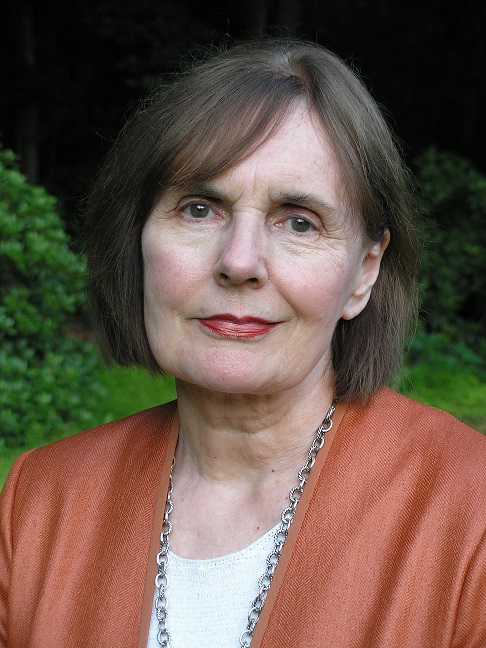
\includegraphics{images/Greta.jpg}

Можно ещё также научиться оценивать визуально, где лежат корни AR и MA (\texttt{unit\ root\ test}). Так как для построенной модели нет AR и MA частей (\texttt{ARIMA\ (0,\ 0,\ 0)}), то можно применить команду к, например, \texttt{ARIMA\ (1,\ 0,\ 0)}:

\begin{Shaded}
\begin{Highlighting}[]
\KeywordTok{autoplot}\NormalTok{(arima_}\DecValTok{100}\NormalTok{)}
\end{Highlighting}
\end{Shaded}

\begin{center}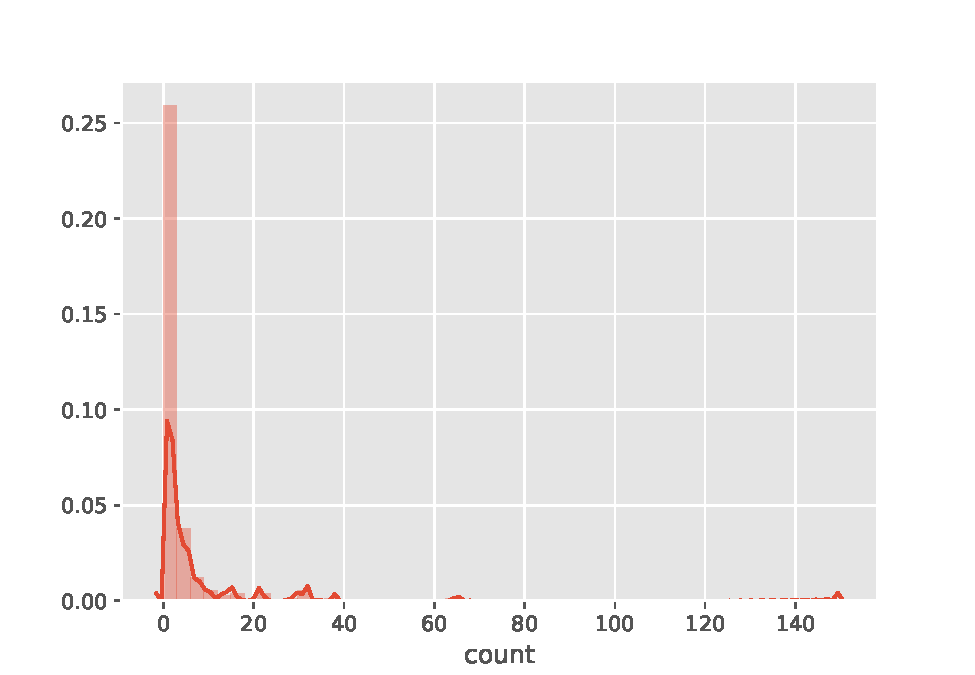
\includegraphics{08-arma_files/figure-latex/unnamed-chunk-12-1} \end{center}

Построим прогноз на 3 периода вперёд для модели \texttt{arima\_000}. Визуализируем прогноз, границы 80\% и 95\% доверительного интервалов.

\begin{Shaded}
\begin{Highlighting}[]
\KeywordTok{forecast}\NormalTok{(arima_}\DecValTok{000}\NormalTok{, }\DataTypeTok{h=}\DecValTok{10}\NormalTok{) }\OperatorTok
\KeywordTok{autoplot}\NormalTok{()}
\end{Highlighting}
\end{Shaded}

\begin{center}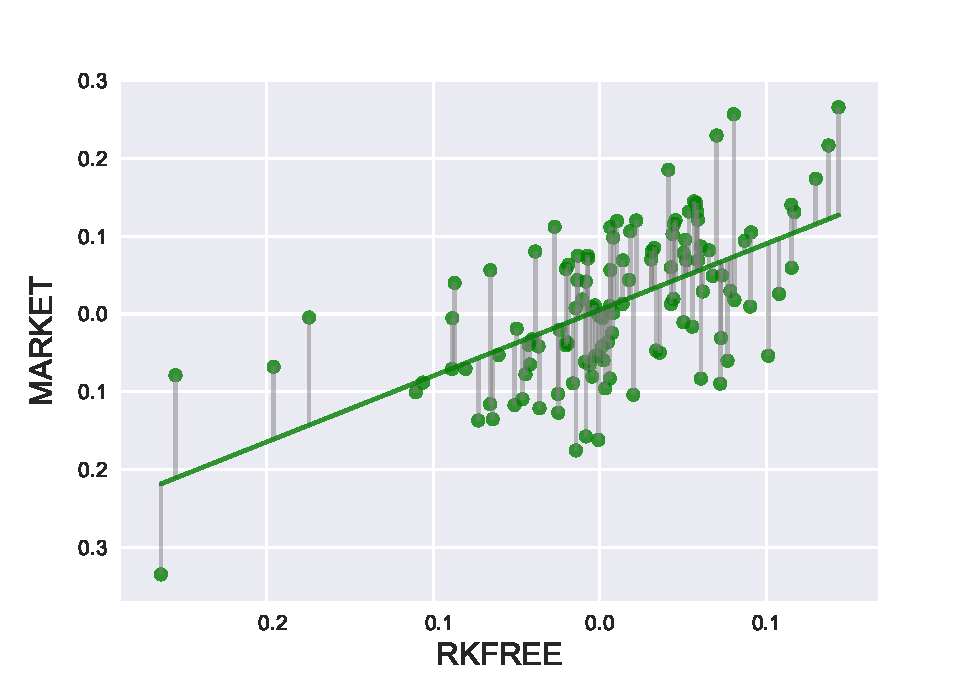
\includegraphics{08-arma_files/figure-latex/unnamed-chunk-13-1} \end{center}

\hypertarget{python-2}{%
\section{python}\label{python-2}}

Настало время \textbf{python}!

Импортируем необходимые пакеты.

\begin{Shaded}
\begin{Highlighting}[]
\ImportTok{import}\NormalTok{ quandl }\CommentTok{# импортирование данных из Сети}
\end{Highlighting}
\end{Shaded}

\begin{verbatim}
Error in py_call_impl(callable, dots$args, dots$keywords): ModuleNotFoundError: No module named 'quandl'

Detailed traceback: 
  File "<string>", line 1, in <module>
\end{verbatim}

\begin{Shaded}
\begin{Highlighting}[]
\ImportTok{import}\NormalTok{ datetime }\CommentTok{# работа с форматами даты и времени}
\ImportTok{import}\NormalTok{ matplotlib.pyplot }\ImportTok{as}\NormalTok{ plt }\CommentTok{# построение графиков}
\end{Highlighting}
\end{Shaded}

\begin{verbatim}
Error in py_call_impl(callable, dots$args, dots$keywords): ModuleNotFoundError: No module named 'matplotlib'

Detailed traceback: 
  File "<string>", line 1, in <module>
\end{verbatim}

\begin{Shaded}
\begin{Highlighting}[]
\ImportTok{from}\NormalTok{ pandas }\ImportTok{import}\NormalTok{ Series }\CommentTok{# работа с временными рядами}
\end{Highlighting}
\end{Shaded}

\begin{verbatim}
Error in py_call_impl(callable, dots$args, dots$keywords): ModuleNotFoundError: No module named 'pandas'

Detailed traceback: 
  File "<string>", line 1, in <module>
\end{verbatim}

\begin{Shaded}
\begin{Highlighting}[]
\ImportTok{import}\NormalTok{ statsmodels}
\end{Highlighting}
\end{Shaded}

\begin{verbatim}
Error in py_call_impl(callable, dots$args, dots$keywords): ModuleNotFoundError: No module named 'statsmodels'

Detailed traceback: 
  File "<string>", line 1, in <module>
\end{verbatim}

\begin{Shaded}
\begin{Highlighting}[]
\ImportTok{from}\NormalTok{ statsmodels.tsa.arima_model }\ImportTok{import}\NormalTok{ ARMA }\CommentTok{# ARMA-модели}
\end{Highlighting}
\end{Shaded}

\begin{verbatim}
Error in py_call_impl(callable, dots$args, dots$keywords): ModuleNotFoundError: No module named 'statsmodels'

Detailed traceback: 
  File "<string>", line 1, in <module>
\end{verbatim}

\begin{Shaded}
\begin{Highlighting}[]
\ImportTok{from}\NormalTok{ statsmodels.graphics.tsaplots }\ImportTok{import}\NormalTok{ plot_acf }\CommentTok{# построение графиков acf и pacf}
\end{Highlighting}
\end{Shaded}

\begin{verbatim}
Error in py_call_impl(callable, dots$args, dots$keywords): ModuleNotFoundError: No module named 'statsmodels'

Detailed traceback: 
  File "<string>", line 1, in <module>
\end{verbatim}

\begin{Shaded}
\begin{Highlighting}[]
\ImportTok{from}\NormalTok{ statsmodels.graphics.tsaplots }\ImportTok{import}\NormalTok{ plot_pacf}
\end{Highlighting}
\end{Shaded}

\begin{verbatim}
Error in py_call_impl(callable, dots$args, dots$keywords): ModuleNotFoundError: No module named 'statsmodels'

Detailed traceback: 
  File "<string>", line 1, in <module>
\end{verbatim}

\begin{Shaded}
\begin{Highlighting}[]
\ImportTok{import}\NormalTok{ statsmodels.api }\ImportTok{as}\NormalTok{ sm}
\end{Highlighting}
\end{Shaded}

\begin{verbatim}
Error in py_call_impl(callable, dots$args, dots$keywords): ModuleNotFoundError: No module named 'statsmodels'

Detailed traceback: 
  File "<string>", line 1, in <module>
\end{verbatim}

\begin{Shaded}
\begin{Highlighting}[]
\ImportTok{from}\NormalTok{ statsmodels.stats }\ImportTok{import}\NormalTok{ diagnostic }\ImportTok{as}\NormalTok{ diag }\CommentTok{# тесты}
\end{Highlighting}
\end{Shaded}

\begin{verbatim}
Error in py_call_impl(callable, dots$args, dots$keywords): ModuleNotFoundError: No module named 'statsmodels'

Detailed traceback: 
  File "<string>", line 1, in <module>
\end{verbatim}

\begin{Shaded}
\begin{Highlighting}[]
\ImportTok{import}\NormalTok{ pmdarima }\ImportTok{as}\NormalTok{ pm}
\end{Highlighting}
\end{Shaded}

\begin{verbatim}
Error in py_call_impl(callable, dots$args, dots$keywords): ModuleNotFoundError: No module named 'pmdarima'

Detailed traceback: 
  File "<string>", line 1, in <module>
\end{verbatim}

\begin{Shaded}
\begin{Highlighting}[]
\ImportTok{from}\NormalTok{ pmdarima.arima }\ImportTok{import}\NormalTok{ auto_arima }\CommentTok{# автоподбор коэффициентов модели ARIMA}
\end{Highlighting}
\end{Shaded}

\begin{verbatim}
Error in py_call_impl(callable, dots$args, dots$keywords): ModuleNotFoundError: No module named 'pmdarima'

Detailed traceback: 
  File "<string>", line 1, in <module>
\end{verbatim}

\begin{Shaded}
\begin{Highlighting}[]
\ImportTok{from}\NormalTok{ statsmodels.tsa.stattools }\ImportTok{import}\NormalTok{ adfuller }\CommentTok{# тест Дики-Фуллера}
\end{Highlighting}
\end{Shaded}

\begin{verbatim}
Error in py_call_impl(callable, dots$args, dots$keywords): ModuleNotFoundError: No module named 'statsmodels'

Detailed traceback: 
  File "<string>", line 1, in <module>
\end{verbatim}

Загрузим dataset:

\begin{Shaded}
\begin{Highlighting}[]
\NormalTok{start }\OperatorTok{=}\NormalTok{ datetime.datetime(}\DecValTok{2015}\NormalTok{, }\DecValTok{1}\NormalTok{, }\DecValTok{1}\NormalTok{)}
\NormalTok{end }\OperatorTok{=}\NormalTok{ datetime.datetime(}\DecValTok{2015}\NormalTok{, }\DecValTok{12}\NormalTok{, }\DecValTok{31}\NormalTok{)}
\NormalTok{apple }\OperatorTok{=}\NormalTok{ quandl.get(}\StringTok{"WIKI/"} \OperatorTok{+} \StringTok{"AAPL"}\NormalTok{, start_date}\OperatorTok{=}\NormalTok{start, end_date}\OperatorTok{=}\NormalTok{end)}
\end{Highlighting}
\end{Shaded}

\begin{verbatim}
Error in py_call_impl(callable, dots$args, dots$keywords): NameError: name 'quandl' is not defined

Detailed traceback: 
  File "<string>", line 1, in <module>
\end{verbatim}

Проверим загрузку данных. Установим dataset как цену закрытия.

\begin{Shaded}
\begin{Highlighting}[]
\NormalTok{apple.head()}
\end{Highlighting}
\end{Shaded}

\begin{verbatim}
Error in py_call_impl(callable, dots$args, dots$keywords): NameError: name 'apple' is not defined

Detailed traceback: 
  File "<string>", line 1, in <module>
\end{verbatim}

\begin{Shaded}
\begin{Highlighting}[]
\NormalTok{apple_df }\OperatorTok{=}\NormalTok{ apple[}\StringTok{"Close"}\NormalTok{]}
\end{Highlighting}
\end{Shaded}

\begin{verbatim}
Error in py_call_impl(callable, dots$args, dots$keywords): NameError: name 'apple' is not defined

Detailed traceback: 
  File "<string>", line 1, in <module>
\end{verbatim}

Посмотрим на структуру временного ряда, автокорреляционную и частную автокорреляционную функции.

\begin{Shaded}
\begin{Highlighting}[]
\NormalTok{apple_df.plot(grid}\OperatorTok{=}\VariableTok{True}\NormalTok{)}
\end{Highlighting}
\end{Shaded}

\begin{verbatim}
Error in py_call_impl(callable, dots$args, dots$keywords): NameError: name 'apple_df' is not defined

Detailed traceback: 
  File "<string>", line 1, in <module>
\end{verbatim}

\begin{Shaded}
\begin{Highlighting}[]
\NormalTok{plt.title(}\StringTok{"Структурa временного ряда"}\NormalTok{)}
\end{Highlighting}
\end{Shaded}

\begin{verbatim}
Error in py_call_impl(callable, dots$args, dots$keywords): NameError: name 'plt' is not defined

Detailed traceback: 
  File "<string>", line 1, in <module>
\end{verbatim}

\begin{Shaded}
\begin{Highlighting}[]
\NormalTok{plt.show()}
\end{Highlighting}
\end{Shaded}

\begin{verbatim}
Error in py_call_impl(callable, dots$args, dots$keywords): NameError: name 'plt' is not defined

Detailed traceback: 
  File "<string>", line 1, in <module>
\end{verbatim}

\begin{Shaded}
\begin{Highlighting}[]
\NormalTok{plot_acf(apple_df, lags}\OperatorTok{=}\DecValTok{20}\NormalTok{)}
\end{Highlighting}
\end{Shaded}

\begin{verbatim}
Error in py_call_impl(callable, dots$args, dots$keywords): NameError: name 'plot_acf' is not defined

Detailed traceback: 
  File "<string>", line 1, in <module>
\end{verbatim}

\begin{Shaded}
\begin{Highlighting}[]
\NormalTok{plt.show()}
\end{Highlighting}
\end{Shaded}

\begin{verbatim}
Error in py_call_impl(callable, dots$args, dots$keywords): NameError: name 'plt' is not defined

Detailed traceback: 
  File "<string>", line 1, in <module>
\end{verbatim}

\begin{Shaded}
\begin{Highlighting}[]
\NormalTok{plot_pacf(apple_df, lags}\OperatorTok{=}\DecValTok{20}\NormalTok{)}
\end{Highlighting}
\end{Shaded}

\begin{verbatim}
Error in py_call_impl(callable, dots$args, dots$keywords): NameError: name 'plot_pacf' is not defined

Detailed traceback: 
  File "<string>", line 1, in <module>
\end{verbatim}

\begin{Shaded}
\begin{Highlighting}[]
\NormalTok{plt.show()}
\end{Highlighting}
\end{Shaded}

\begin{verbatim}
Error in py_call_impl(callable, dots$args, dots$keywords): NameError: name 'plt' is not defined

Detailed traceback: 
  File "<string>", line 1, in <module>
\end{verbatim}

Появились очень знакомые (и красивые) графики. Важно отметить, что на графиках есть 0 - лаг, он равен единице, в предыдущих графиках его не было.

Проверим стационарность ряда тестом Дики-Фуллера.

\begin{Shaded}
\begin{Highlighting}[]
\NormalTok{res }\OperatorTok{=}\NormalTok{ sm.tsa.adfuller(apple_df, regression}\OperatorTok{=}\StringTok{'ct'}\NormalTok{)}
\end{Highlighting}
\end{Shaded}

\begin{verbatim}
Error in py_call_impl(callable, dots$args, dots$keywords): NameError: name 'sm' is not defined

Detailed traceback: 
  File "<string>", line 1, in <module>
\end{verbatim}

\begin{Shaded}
\begin{Highlighting}[]
\CommentTok{'p-value:\{\}'}\NormalTok{.}\BuiltInTok{format}\NormalTok{(res[}\DecValTok{1}\NormalTok{])}
\end{Highlighting}
\end{Shaded}

\begin{verbatim}
Error in py_call_impl(callable, dots$args, dots$keywords): NameError: name 'res' is not defined

Detailed traceback: 
  File "<string>", line 1, in <module>
\end{verbatim}

Возьмём первую разность.

\begin{Shaded}
\begin{Highlighting}[]
\NormalTok{apple_diff }\OperatorTok{=}\NormalTok{ apple_df.diff(periods}\OperatorTok{=}\DecValTok{1}\NormalTok{).dropna()}
\end{Highlighting}
\end{Shaded}

\begin{verbatim}
Error in py_call_impl(callable, dots$args, dots$keywords): NameError: name 'apple_df' is not defined

Detailed traceback: 
  File "<string>", line 1, in <module>
\end{verbatim}

И визуализируем структуру нового ряда.

\begin{Shaded}
\begin{Highlighting}[]
\NormalTok{apple_diff.plot(grid}\OperatorTok{=}\VariableTok{True}\NormalTok{)}
\end{Highlighting}
\end{Shaded}

\begin{verbatim}
Error in py_call_impl(callable, dots$args, dots$keywords): NameError: name 'apple_diff' is not defined

Detailed traceback: 
  File "<string>", line 1, in <module>
\end{verbatim}

\begin{Shaded}
\begin{Highlighting}[]
\NormalTok{plt.title(}\StringTok{"Структурa временного ряда"}\NormalTok{)}
\end{Highlighting}
\end{Shaded}

\begin{verbatim}
Error in py_call_impl(callable, dots$args, dots$keywords): NameError: name 'plt' is not defined

Detailed traceback: 
  File "<string>", line 1, in <module>
\end{verbatim}

\begin{Shaded}
\begin{Highlighting}[]
\NormalTok{plt.show()}
\end{Highlighting}
\end{Shaded}

\begin{verbatim}
Error in py_call_impl(callable, dots$args, dots$keywords): NameError: name 'plt' is not defined

Detailed traceback: 
  File "<string>", line 1, in <module>
\end{verbatim}

\begin{Shaded}
\begin{Highlighting}[]
\NormalTok{plot_acf(apple_diff, lags}\OperatorTok{=}\DecValTok{50}\NormalTok{)}
\end{Highlighting}
\end{Shaded}

\begin{verbatim}
Error in py_call_impl(callable, dots$args, dots$keywords): NameError: name 'plot_acf' is not defined

Detailed traceback: 
  File "<string>", line 1, in <module>
\end{verbatim}

\begin{Shaded}
\begin{Highlighting}[]
\NormalTok{plt.show()}
\end{Highlighting}
\end{Shaded}

\begin{verbatim}
Error in py_call_impl(callable, dots$args, dots$keywords): NameError: name 'plt' is not defined

Detailed traceback: 
  File "<string>", line 1, in <module>
\end{verbatim}

\begin{Shaded}
\begin{Highlighting}[]
\NormalTok{plot_pacf(apple_diff, lags}\OperatorTok{=}\DecValTok{50}\NormalTok{)}
\end{Highlighting}
\end{Shaded}

\begin{verbatim}
Error in py_call_impl(callable, dots$args, dots$keywords): NameError: name 'plot_pacf' is not defined

Detailed traceback: 
  File "<string>", line 1, in <module>
\end{verbatim}

\begin{Shaded}
\begin{Highlighting}[]
\NormalTok{plt.show()}
\end{Highlighting}
\end{Shaded}

\begin{verbatim}
Error in py_call_impl(callable, dots$args, dots$keywords): NameError: name 'plt' is not defined

Detailed traceback: 
  File "<string>", line 1, in <module>
\end{verbatim}

Аналогично операциям в \textbf{r}, смоделируем данный ряд как \texttt{ARMA\ (0,\ 0)}.

\begin{Shaded}
\begin{Highlighting}[]
\NormalTok{arma_00 }\OperatorTok{=}\NormalTok{ ARMA(apple_diff, order}\OperatorTok{=}\NormalTok{(}\DecValTok{0}\NormalTok{, }\DecValTok{0}\NormalTok{))}
\end{Highlighting}
\end{Shaded}

\begin{verbatim}
Error in py_call_impl(callable, dots$args, dots$keywords): NameError: name 'ARMA' is not defined

Detailed traceback: 
  File "<string>", line 1, in <module>
\end{verbatim}

\begin{Shaded}
\begin{Highlighting}[]
\NormalTok{arma_00_fit }\OperatorTok{=}\NormalTok{ arma_00.fit(disp}\OperatorTok{=}\VariableTok{False}\NormalTok{)}
\end{Highlighting}
\end{Shaded}

\begin{verbatim}
Error in py_call_impl(callable, dots$args, dots$keywords): NameError: name 'arma_00' is not defined

Detailed traceback: 
  File "<string>", line 1, in <module>
\end{verbatim}

\begin{Shaded}
\begin{Highlighting}[]
\NormalTok{arma_00_fit.summary()}
\end{Highlighting}
\end{Shaded}

\begin{verbatim}
Error in py_call_impl(callable, dots$args, dots$keywords): NameError: name 'arma_00_fit' is not defined

Detailed traceback: 
  File "<string>", line 1, in <module>
\end{verbatim}

Смоделируем ряд как \texttt{ARMA\ (1,\ 0)}:

\begin{Shaded}
\begin{Highlighting}[]
\NormalTok{arma_10 }\OperatorTok{=}\NormalTok{ ARMA(apple_diff, order}\OperatorTok{=}\NormalTok{(}\DecValTok{1}\NormalTok{, }\DecValTok{0}\NormalTok{))}
\end{Highlighting}
\end{Shaded}

\begin{verbatim}
Error in py_call_impl(callable, dots$args, dots$keywords): NameError: name 'ARMA' is not defined

Detailed traceback: 
  File "<string>", line 1, in <module>
\end{verbatim}

\begin{Shaded}
\begin{Highlighting}[]
\NormalTok{arma_10_fit }\OperatorTok{=}\NormalTok{ arma_10.fit(disp}\OperatorTok{=}\VariableTok{False}\NormalTok{)}
\end{Highlighting}
\end{Shaded}

\begin{verbatim}
Error in py_call_impl(callable, dots$args, dots$keywords): NameError: name 'arma_10' is not defined

Detailed traceback: 
  File "<string>", line 1, in <module>
\end{verbatim}

\begin{Shaded}
\begin{Highlighting}[]
\NormalTok{arma_10_fit.summary()}
\end{Highlighting}
\end{Shaded}

\begin{verbatim}
Error in py_call_impl(callable, dots$args, dots$keywords): NameError: name 'arma_10_fit' is not defined

Detailed traceback: 
  File "<string>", line 1, in <module>
\end{verbatim}

Вторая модель имеет более высокое значение критерия Акаике и незначимый коэффициент перед ar(1).

Отдельно можно выделить значения AIC и BIC для построенных моделей.

\begin{Shaded}
\begin{Highlighting}[]
\NormalTok{np.}\BuiltInTok{round}\NormalTok{(arma_00_fit.aic, }\DecValTok{2}\NormalTok{)}
\end{Highlighting}
\end{Shaded}

\begin{verbatim}
Error in py_call_impl(callable, dots$args, dots$keywords): NameError: name 'np' is not defined

Detailed traceback: 
  File "<string>", line 1, in <module>
\end{verbatim}

\begin{Shaded}
\begin{Highlighting}[]
\NormalTok{np.}\BuiltInTok{round}\NormalTok{(arma_10_fit.aic, }\DecValTok{2}\NormalTok{)}
\end{Highlighting}
\end{Shaded}

\begin{verbatim}
Error in py_call_impl(callable, dots$args, dots$keywords): NameError: name 'np' is not defined

Detailed traceback: 
  File "<string>", line 1, in <module>
\end{verbatim}

\begin{Shaded}
\begin{Highlighting}[]
\NormalTok{np.}\BuiltInTok{round}\NormalTok{(arma_00_fit.bic, }\DecValTok{2}\NormalTok{)}
\end{Highlighting}
\end{Shaded}

\begin{verbatim}
Error in py_call_impl(callable, dots$args, dots$keywords): NameError: name 'np' is not defined

Detailed traceback: 
  File "<string>", line 1, in <module>
\end{verbatim}

\begin{Shaded}
\begin{Highlighting}[]
\NormalTok{np.}\BuiltInTok{round}\NormalTok{(arma_10_fit.bic, }\DecValTok{2}\NormalTok{)}
\end{Highlighting}
\end{Shaded}

\begin{verbatim}
Error in py_call_impl(callable, dots$args, dots$keywords): NameError: name 'np' is not defined

Detailed traceback: 
  File "<string>", line 1, in <module>
\end{verbatim}

Как и в \textbf{r}, \textbf{python} имеет опцию автоподбора коэффициентов модели \texttt{ARIMA}.

\begin{Shaded}
\begin{Highlighting}[]
\NormalTok{auto_arima_python }\OperatorTok{=}\NormalTok{ pm.auto_arima(apple_diff)}
\end{Highlighting}
\end{Shaded}

\begin{verbatim}
Error in py_call_impl(callable, dots$args, dots$keywords): NameError: name 'pm' is not defined

Detailed traceback: 
  File "<string>", line 1, in <module>
\end{verbatim}

\begin{Shaded}
\begin{Highlighting}[]
\NormalTok{auto_arima_python.summary()}
\end{Highlighting}
\end{Shaded}

\begin{verbatim}
Error in py_call_impl(callable, dots$args, dots$keywords): NameError: name 'auto_arima_python' is not defined

Detailed traceback: 
  File "<string>", line 1, in <module>
\end{verbatim}

В строчке \texttt{SARIMAX} нет рядом коэффициентов. Это означает, что они нулевые, как и предполагалось, то есть модель описывается \texttt{ARMA\ (0,\ 0)}.Эта функция также удобна тем, что выводит статистики.

Проверим белошумность остатков тестом Льюнг - Бокса.

Сначала сохраним остатки как \texttt{residuals}.

\begin{Shaded}
\begin{Highlighting}[]
\NormalTok{residuals }\OperatorTok{=}\NormalTok{ pd.DataFrame(arma_00_fit.resid)}
\end{Highlighting}
\end{Shaded}

\begin{verbatim}
Error in py_call_impl(callable, dots$args, dots$keywords): NameError: name 'pd' is not defined

Detailed traceback: 
  File "<string>", line 1, in <module>
\end{verbatim}

\begin{Shaded}
\begin{Highlighting}[]
\NormalTok{diag.acorr_ljungbox(residuals, lags}\OperatorTok{=}\DecValTok{10}\NormalTok{, boxpierce}\OperatorTok{=}\VariableTok{False}\NormalTok{)}
\end{Highlighting}
\end{Shaded}

\begin{verbatim}
Error in py_call_impl(callable, dots$args, dots$keywords): NameError: name 'diag' is not defined

Detailed traceback: 
  File "<string>", line 1, in <module>
\end{verbatim}

Посмотрим на прогноз на 10 дней вперёд.

\begin{Shaded}
\begin{Highlighting}[]
\NormalTok{forecast }\OperatorTok{=}\NormalTok{ arma_00_fit.forecast(steps}\OperatorTok{=}\DecValTok{10}\NormalTok{)[}\DecValTok{0}\NormalTok{]}
\end{Highlighting}
\end{Shaded}

\begin{verbatim}
Error in py_call_impl(callable, dots$args, dots$keywords): NameError: name 'arma_00_fit' is not defined

Detailed traceback: 
  File "<string>", line 1, in <module>
\end{verbatim}

\begin{Shaded}
\begin{Highlighting}[]
\NormalTok{forecast}
\end{Highlighting}
\end{Shaded}

\begin{verbatim}
Error in py_call_impl(callable, dots$args, dots$keywords): NameError: name 'forecast' is not defined

Detailed traceback: 
  File "<string>", line 1, in <module>
\end{verbatim}

И визуализируем прогнозные значения на исходном графике.

\begin{Shaded}
\begin{Highlighting}[]
\NormalTok{arma_00_fit.plot_predict(}\BuiltInTok{len}\NormalTok{(apple_diff)}\OperatorTok{-}\DecValTok{250}\NormalTok{, }\BuiltInTok{len}\NormalTok{(apple_diff)}\OperatorTok{+}\DecValTok{10}\NormalTok{)}
\end{Highlighting}
\end{Shaded}

\begin{verbatim}
Error in py_call_impl(callable, dots$args, dots$keywords): NameError: name 'arma_00_fit' is not defined

Detailed traceback: 
  File "<string>", line 1, in <module>
\end{verbatim}

\begin{Shaded}
\begin{Highlighting}[]
\NormalTok{plt.xlabel(}\StringTok{'Лаги'}\NormalTok{)}
\end{Highlighting}
\end{Shaded}

\begin{verbatim}
Error in py_call_impl(callable, dots$args, dots$keywords): NameError: name 'plt' is not defined

Detailed traceback: 
  File "<string>", line 1, in <module>
\end{verbatim}

\begin{Shaded}
\begin{Highlighting}[]
\NormalTok{plt.ylabel(}\StringTok{'Изменение цены'}\NormalTok{)}
\end{Highlighting}
\end{Shaded}

\begin{verbatim}
Error in py_call_impl(callable, dots$args, dots$keywords): NameError: name 'plt' is not defined

Detailed traceback: 
  File "<string>", line 1, in <module>
\end{verbatim}

\begin{Shaded}
\begin{Highlighting}[]
\NormalTok{plt.title(}\StringTok{'Изменение цены закрытия AAPL'}\NormalTok{)}
\end{Highlighting}
\end{Shaded}

\begin{verbatim}
Error in py_call_impl(callable, dots$args, dots$keywords): NameError: name 'plt' is not defined

Detailed traceback: 
  File "<string>", line 1, in <module>
\end{verbatim}

\begin{Shaded}
\begin{Highlighting}[]
\NormalTok{plt.show()}
\end{Highlighting}
\end{Shaded}

\begin{verbatim}
Error in py_call_impl(callable, dots$args, dots$keywords): NameError: name 'plt' is not defined

Detailed traceback: 
  File "<string>", line 1, in <module>
\end{verbatim}

\hypertarget{stata-2}{%
\section{stata}\label{stata-2}}

Теперь научимся анализировать временные ряды в \textbf{stata}.
Импортируем dataset.

\begin{verbatim}
use data/apple.dta
\end{verbatim}

Установим временной формат переменной \texttt{Date} и визуализируем исследуемый временной ряд, его автокорреляционную и частную автокорреляционную функции.

\begin{verbatim}
tsset Date
\end{verbatim}

\begin{verbatim}
 file data/apple.dta not found
r(601);


no variables defined
r(111);

end of do-file
r(111);
\end{verbatim}

\begin{verbatim}
tsline Close
\end{verbatim}

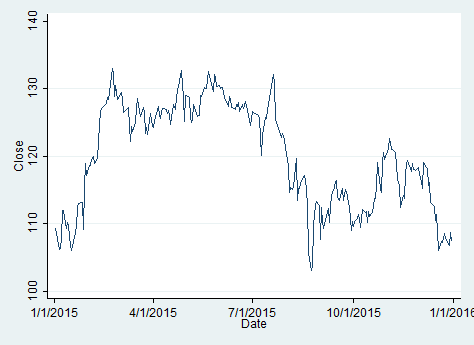
\includegraphics{ts.png}

\begin{verbatim}
ac Close
\end{verbatim}

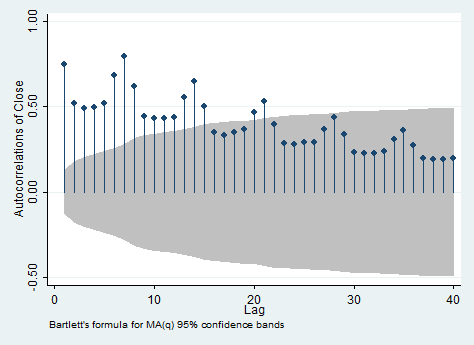
\includegraphics{ac.png}

\begin{verbatim}
pac Close
\end{verbatim}

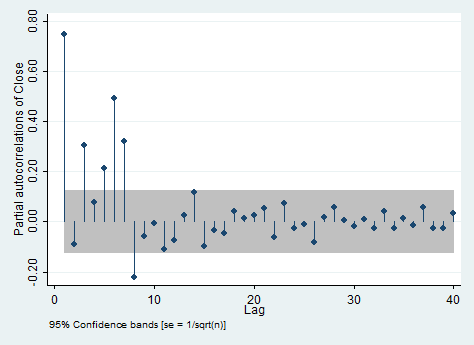
\includegraphics{pac.png}

Проверим стационарность ряда тестом Дики-Фуллера.

\begin{verbatim}
dfuller Close, trend lags(0)
\end{verbatim}

\begin{verbatim}
 file data/apple.dta not found
r(601);


no variables defined
r(111);

end of do-file
r(111);
\end{verbatim}

Тест выявил нестационарность на 5\% уровне значимости (основная гипотеза - о нестационарности).
Возьмём первую разность от ряда, чтобы сделать его стационарным и снова построим графики ACF и PACF.

\begin{verbatim}
gen Close_1 = Close[_n]-Close[_n-1]
\end{verbatim}

И визуализируем его, вместе с автокорреляционной и частной автокорреляционной функциями.

\begin{verbatim}
tsline Close_1
\end{verbatim}

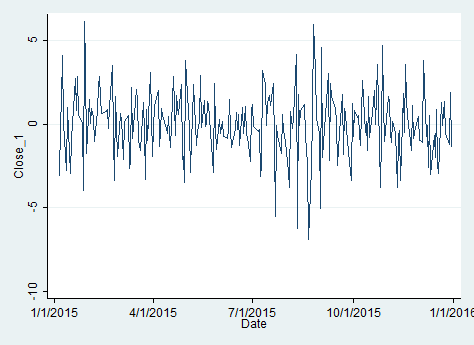
\includegraphics{ts_1.png}

\begin{verbatim}
ac Close_1
\end{verbatim}

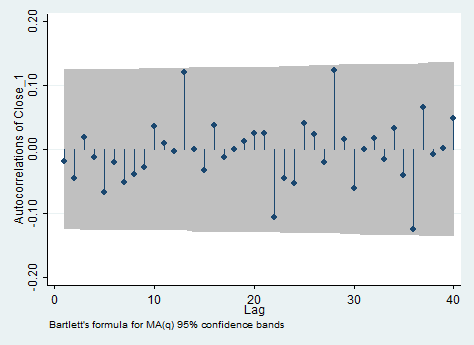
\includegraphics{acc_1.png}

\begin{verbatim}
pac Close_1
\end{verbatim}

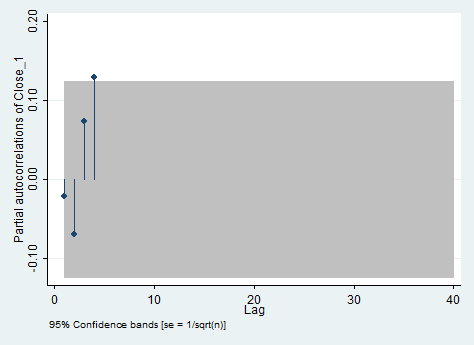
\includegraphics{pacc_1.png}

Теперь построим несколько моделей, которые потенциально могут описать данный ряд, хотя уже заранее ожидается, что ряд в разностях будет описан \texttt{ARIMA\ (0,\ 0,\ 0)}, что равносильно \texttt{ARMA\ (0,\ 0)}, но всё же\ldots{}
\texttt{ARIMA\ (0,\ 0,\ 0)}.Можно также отдельно вывести AIC и BIC для построенной модели. Построим также модель \texttt{ARIMA\ (1,\ 0,\ 0)} для сравнения.

\begin{verbatim}
arima Close_1, arima(0, 0, 0)
estat ic
arima Close_1, arima(1, 0, 0)
estat ic
\end{verbatim}

\begin{verbatim}
 file data/apple.dta not found
r(601);


no variables defined
r(111);

end of do-file
r(111);
\end{verbatim}

По информационному критерию Акаике первая модель лучше (AIC меньше), а также во второй модели коэффициент перед ar(1) незначим.
Проверим остатки модели \texttt{ARIMA\ (0,\ 0,\ 0)} на белошумность. Сохраним остатки модели и проверим тестом Льюнг-Бокса. Основная гипотеза - остатки независимы.

\begin{verbatim}
arima Close_1, arima(0, 0, 0)
predict res, resid
wntestq res
\end{verbatim}

\begin{verbatim}
 file data/apple.dta not found
r(601);


no variables defined
r(111);

end of do-file
r(111);
\end{verbatim}

Теперь попробуем построить прогноз по модели \texttt{ARIMA\ (0,\ 0,\ 0)}:

\begin{verbatim}
arima Close_1, arima(0, 0, 0)
predict prognoz
display prognoz
\end{verbatim}

\begin{verbatim}
 file data/apple.dta not found
r(601);


no variables defined
r(111);

end of do-file
r(111);
\end{verbatim}

\hypertarget{paneldata}{%
\chapter{Панельные данные}\label{paneldata}}

Загрузим необходимые библиотеки.

\begin{Shaded}
\begin{Highlighting}[]
\KeywordTok{library}\NormalTok{(foreign) }\CommentTok{#Вспомогательная библиотека для подгрузки данных}
\KeywordTok{library}\NormalTok{(plm) }\CommentTok{#Пакет для работы с панельными данными}
\KeywordTok{library}\NormalTok{(lmtest) }\CommentTok{#Пакет для оценки регрессий и ковариационных матриц параметров}
\KeywordTok{library}\NormalTok{(skimr) }\CommentTok{#Для красивого summary}
\KeywordTok{library}\NormalTok{(car) }\CommentTok{#Для некоторых графиков}
\KeywordTok{library}\NormalTok{(gplots) }\CommentTok{#Для графигов гетерогенности}
\KeywordTok{library}\NormalTok{(rio)}
\KeywordTok{library}\NormalTok{(tidyverse)}
\KeywordTok{library}\NormalTok{(car)}
\end{Highlighting}
\end{Shaded}

Загрузим данные, и преобразуем нужные переменные в факторные.В данном разделе все визуализации будут построены на подмножестве данных из шести наблюдений. Это позволит сделать их более читаемыми в формате книги. Все модели будут оценены на всём массиве данных.

\begin{Shaded}
\begin{Highlighting}[]
\NormalTok{panel =}\StringTok{ }\KeywordTok{read_csv}\NormalTok{(}\StringTok{'lwage_panel_small.csv'}\NormalTok{)}
\NormalTok{panel}\OperatorTok{$}\NormalTok{black =}\StringTok{ }\KeywordTok{factor}\NormalTok{(panel}\OperatorTok{$}\NormalTok{black)}
\NormalTok{panel}\OperatorTok{$}\NormalTok{id =}\StringTok{ }\KeywordTok{factor}\NormalTok{(panel}\OperatorTok{$}\NormalTok{id)}
\end{Highlighting}
\end{Shaded}

Изобразим наши панельные данные на диаграмме рассеяния. Дополнимельно установим параметр сглаживания, чтобы получить кривые временных рядов.

\begin{Shaded}
\begin{Highlighting}[]
\KeywordTok{scatterplot}\NormalTok{(lwage }\OperatorTok{~}\StringTok{ }\NormalTok{year}\OperatorTok{|}\NormalTok{id, }\DataTypeTok{boxplots=}\NormalTok{F, }\DataTypeTok{smooth=}\OtherTok{TRUE}\NormalTok{, }\DataTypeTok{regLine=}\OtherTok{FALSE}\NormalTok{, }\DataTypeTok{data=}\NormalTok{panel)}
\end{Highlighting}
\end{Shaded}

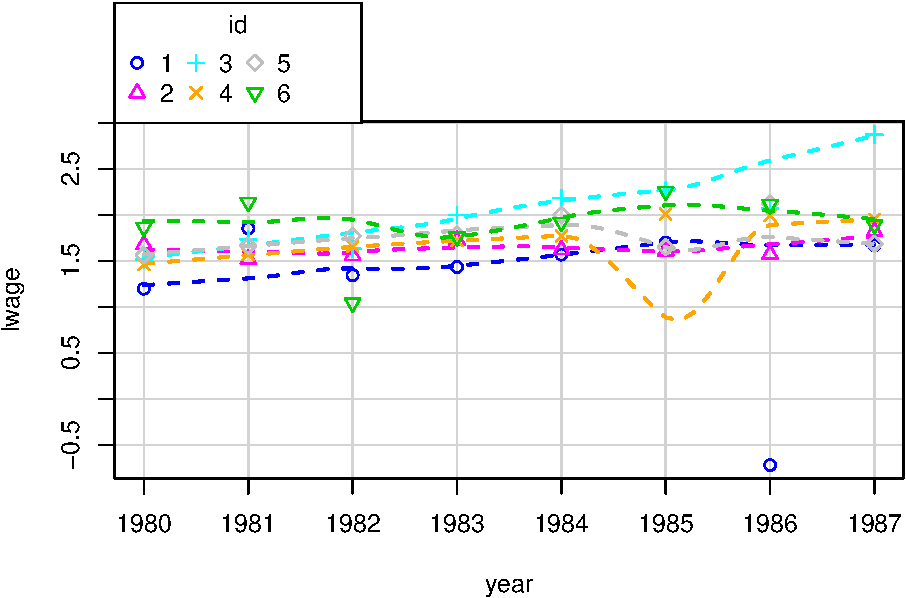
\includegraphics{09-paneldata_files/figure-latex/scatterplot chunk-1.pdf}

Для получения графиков на различных плитках можно использовать coplot.

\begin{Shaded}
\begin{Highlighting}[]
\KeywordTok{coplot}\NormalTok{(lwage }\OperatorTok{~}\StringTok{ }\NormalTok{year}\OperatorTok{|}\NormalTok{id, }\DataTypeTok{type =} \StringTok{'b'}\NormalTok{, }\DataTypeTok{data =}\NormalTok{ panel)}
\end{Highlighting}
\end{Shaded}

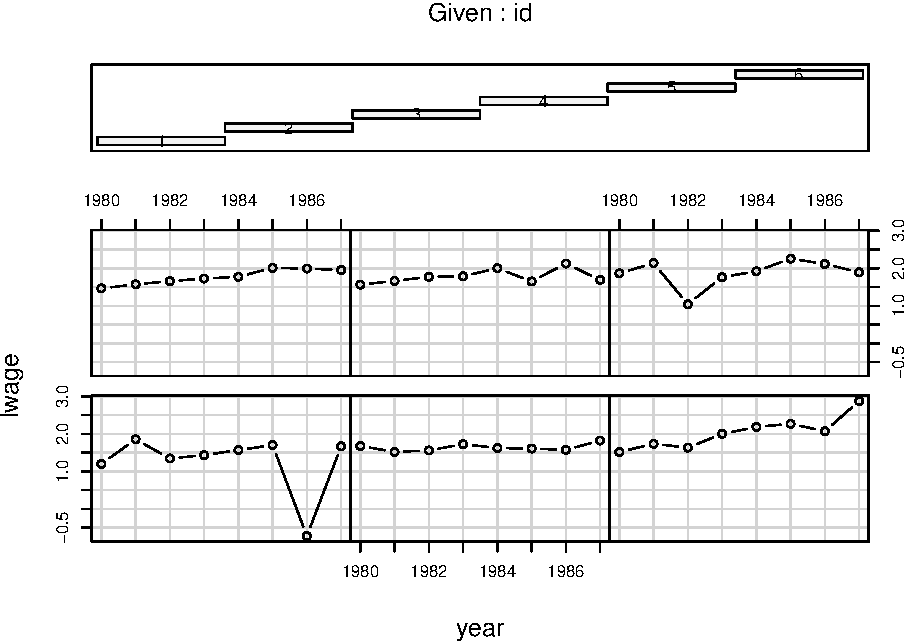
\includegraphics{09-paneldata_files/figure-latex/1 coplot chunk-1.pdf}

Сгруппировать можно по разным признакам. Например, в зависимости от расы индивидов.

\begin{Shaded}
\begin{Highlighting}[]
\NormalTok{panel}\OperatorTok{$}\NormalTok{year =}\StringTok{ }\KeywordTok{factor}\NormalTok{(panel}\OperatorTok{$}\NormalTok{year)}
\KeywordTok{coplot}\NormalTok{(lwage }\OperatorTok{~}\StringTok{ }\NormalTok{year}\OperatorTok{|}\NormalTok{black, }\DataTypeTok{type=}\StringTok{"l"}\NormalTok{, }\DataTypeTok{data=}\NormalTok{panel, }\DataTypeTok{panel =} \ControlFlowTok{function}\NormalTok{(x, y, ...) }\KeywordTok{panel.smooth}\NormalTok{(x, y, }\DataTypeTok{span =} \FloatTok{0.3}\NormalTok{, ...), }\DataTypeTok{pch =} \DecValTok{16}\NormalTok{, }\DataTypeTok{show.given =}\NormalTok{ F, }\DataTypeTok{xlab =} \StringTok{"Mean dependence lwage of year for white and black people"}\NormalTok{)}
\end{Highlighting}
\end{Shaded}

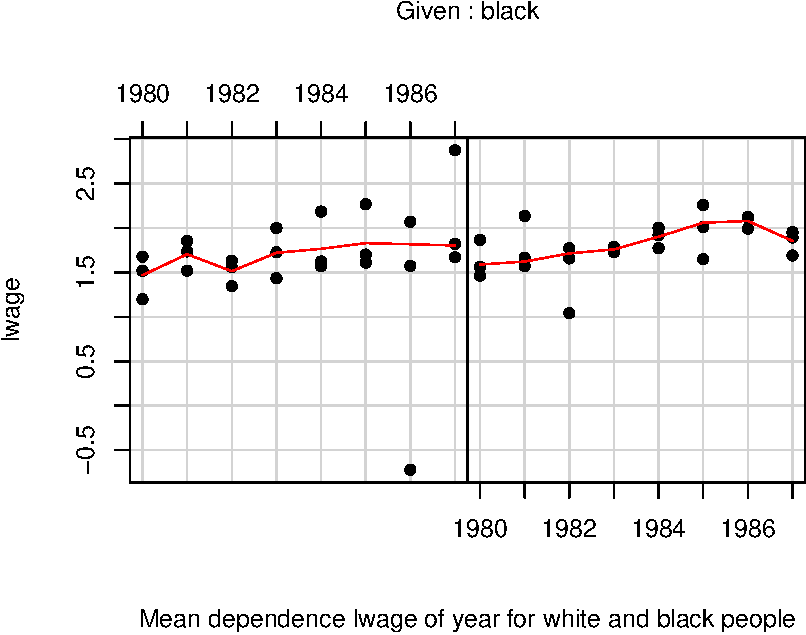
\includegraphics{09-paneldata_files/figure-latex/2 coplot chunk-1.pdf}

Импортируем основной датасет.

\begin{Shaded}
\begin{Highlighting}[]
\NormalTok{Panel =}\StringTok{ }\KeywordTok{import}\NormalTok{(}\StringTok{'lwage_panel_large.csv'}\NormalTok{)}
\end{Highlighting}
\end{Shaded}

Визуализируем гетерогенный эффект. Можно визуализировать по годам или по индивидам. Здесь уже можно использовать полный датасет. Так как доверительные интервалы с интервалом в год не пересекаются, можно увидеть явную гетерогенность.

\begin{Shaded}
\begin{Highlighting}[]
\KeywordTok{plotmeans}\NormalTok{(lwage }\OperatorTok{~}\StringTok{ }\NormalTok{year, }\DataTypeTok{main=}\StringTok{"Heterogeineity across years"}\NormalTok{, }\DataTypeTok{data=}\NormalTok{Panel)}
\end{Highlighting}
\end{Shaded}

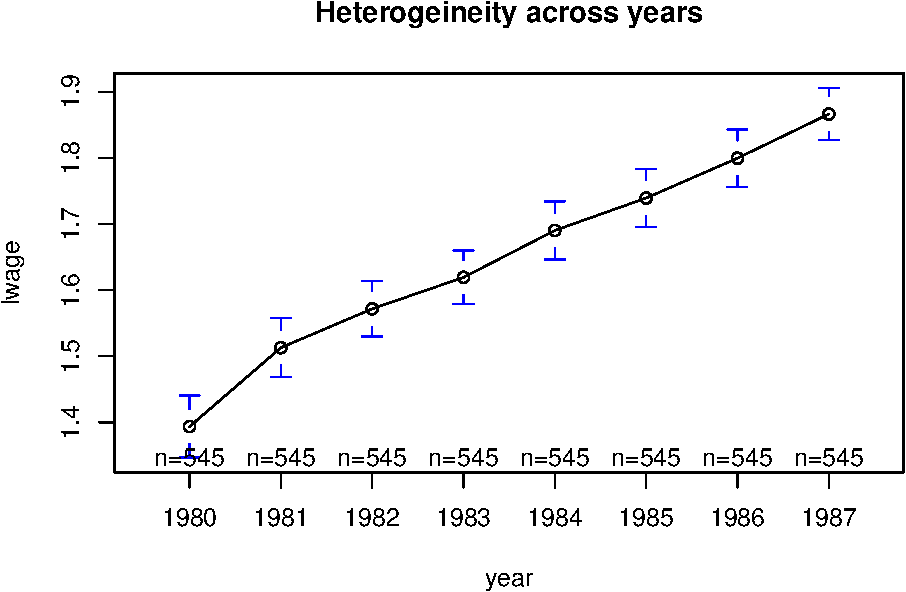
\includegraphics{09-paneldata_files/figure-latex/heterogenity plot-1.pdf}

Модель панельных данных будет выглядеть следующим образом:

\begin{equation}
y_{i t}=\alpha+x_{i t}^{\prime} \beta+z_{i}^{\prime} \gamma+c_{i}+u_{i t}
\end{equation}

где \(\alpha\) -- константа, \(c_{i}\) - индивидуальные эффекты индивидов, а \(z_i\) -- независимые от времени переменные. Следовательно, матрица \(X\) - матрица зависимых от времени регрессов, \(Z\) - матрица независимых от времени регрессоров. Дополнительно обозначим как \(l_n\) вектор из единиц.

Оценим простую модель с фиксированными эффектами через within-оценку. Вычитая \(\overline{y}_{i}=1 / T \sum_{t} y_{i t}\) из исходной модели, получим within-модель:

\begin{equation}
\ddot{y}_{i t}=\ddot{x}_{i t}^{\prime} \beta+\ddot{u}_{i t}
\end{equation}

где \(\ddot{y}_{i t}=y_{i t}-\overline{y}_{i}, \ddot{x}_{i t k}=x_{i t k}-\overline{x}_{i k}\) and \(\ddot{u}_{i t}=u_{i t}-\overline{u}_{i}\). Следует заметить, что константа \(\alpha\), индивидуальные эффекты \(c_i\) и инвариантные ко времени регрессоры \(z_i\) исчезают из модели.

\begin{equation}
\widehat{\beta}_{F E}=\left(\ddot{X}^{\prime} \ddot{X}\right)^{-1} \ddot{X}^{\prime} \ddot{y}
\end{equation}

\begin{Shaded}
\begin{Highlighting}[]
\NormalTok{ffe =}\StringTok{ }\KeywordTok{plm}\NormalTok{(lwage }\OperatorTok{~}\StringTok{ }\NormalTok{hours, }\DataTypeTok{model=}\StringTok{"within"}\NormalTok{, }\DataTypeTok{data =}\NormalTok{ Panel)}
\KeywordTok{summary}\NormalTok{(ffe)}
\end{Highlighting}
\end{Shaded}

\begin{verbatim}
Oneway (individual) effect Within Model

Call:
plm(formula = lwage ~ hours, data = Panel, model = "within")

Balanced Panel: n = 545, T = 8, N = 4360

Residuals:
     Min.   1st Qu.    Median   3rd Qu.      Max. 
-4.116091 -0.136963  0.015755  0.182507  1.555059 

Coefficients:
         Estimate  Std. Error t-value Pr(>|t|)
hours -5.5854e-07  1.4013e-05 -0.0399   0.9682

Total Sum of Squares:    572.05
Residual Sum of Squares: 572.05
R-Squared:      4.1656e-07
Adj. R-Squared: -0.14289
F-statistic: 0.00158875 on 1 and 3814 DF, p-value: 0.96821
\end{verbatim}

Проверим значимость коэффициентов, используя ковариационную матрицу ошибок Хубера - Уайта.

\begin{Shaded}
\begin{Highlighting}[]
\KeywordTok{coeftest}\NormalTok{(ffe, }\DataTypeTok{vcov=}\KeywordTok{vcovHC}\NormalTok{(ffe, }\DataTypeTok{cluster=}\StringTok{"group"}\NormalTok{))}
\end{Highlighting}
\end{Shaded}

\begin{verbatim}

t test of coefficients:

         Estimate  Std. Error t value Pr(>|t|)
hours -5.5854e-07  2.5051e-05 -0.0223   0.9822
\end{verbatim}

Оценим модель со случайными эффектами, используя достижимый обобщённый МНК (FGLS).

\begin{equation}
\left(\begin{array}{c}{\widehat{\alpha}_{R E}} \\ {\widehat{\beta}_{R E}} \\ {\widehat{\gamma}_{R E}}\end{array}\right)=\left(W^{\prime} \widehat{\Omega}_{v}^{-1} W\right)^{-1} W^{\prime} \widehat{\Omega}_{v}^{-1} y
\end{equation}

где

\(W=\left[\iota_{N T} X Z\right] \text { и } \iota_{N T} \text { это вектор из единиц размерности } N T \times 1\)

\begin{Shaded}
\begin{Highlighting}[]
\NormalTok{fre =}\StringTok{ }\KeywordTok{plm}\NormalTok{(lwage }\OperatorTok{~}\StringTok{ }\NormalTok{hours, }\DataTypeTok{model=}\StringTok{"random"}\NormalTok{, }\DataTypeTok{data =}\NormalTok{ Panel)}
\KeywordTok{summary}\NormalTok{(fre)}
\end{Highlighting}
\end{Shaded}

\begin{verbatim}
Oneway (individual) effect Random Effect Model 
   (Swamy-Arora's transformation)

Call:
plm(formula = lwage ~ hours, data = Panel, model = "random")

Balanced Panel: n = 545, T = 8, N = 4360

Effects:
                 var std.dev share
idiosyncratic 0.1500  0.3873 0.528
individual    0.1341  0.3663 0.472
theta: 0.6498

Residuals:
     Min.   1st Qu.    Median   3rd Qu.      Max. 
-4.506028 -0.164365  0.028671  0.218928  1.605623 

Coefficients:
              Estimate Std. Error z-value Pr(>|z|)    
(Intercept) 1.6459e+00 3.3705e-02 48.8332   <2e-16 ***
hours       1.4611e-06 1.3348e-05  0.1095   0.9128    
---
Signif. codes:  0 '***' 0.001 '**' 0.01 '*' 0.05 '.' 0.1 ' ' 1

Total Sum of Squares:    653.53
Residual Sum of Squares: 653.53
R-Squared:      2.7494e-06
Adj. R-Squared: -0.00022671
Chisq: 0.0119818 on 1 DF, p-value: 0.91284
\end{verbatim}

Проверим значимость коэффициентов, используя ковариационную матрицу ошибок Хубера - Уайта.

\begin{Shaded}
\begin{Highlighting}[]
\KeywordTok{coeftest}\NormalTok{(fre, }\DataTypeTok{vcov=}\KeywordTok{vcovHC}\NormalTok{(ffe, }\DataTypeTok{cluster=}\StringTok{"group"}\NormalTok{))}
\end{Highlighting}
\end{Shaded}

\begin{verbatim}

t test of coefficients:

        Estimate Std. Error t value Pr(>|t|)
hours 1.4611e-06 2.5051e-05  0.0583   0.9535
\end{verbatim}

Проведём тест Хаусмана

\begin{Shaded}
\begin{Highlighting}[]
\KeywordTok{phtest}\NormalTok{(ffe, fre)}
\end{Highlighting}
\end{Shaded}

\begin{verbatim}

    Hausman Test

data:  lwage ~ hours
chisq = 0.22438, df = 1, p-value = 0.6357
alternative hypothesis: one model is inconsistent
\end{verbatim}

Построим FD-оценку.

\begin{equation}
\dot{y}_{i t}=\dot{x}_{i t}^{\prime} \beta+\dot{u}_{i t}
\end{equation}

\(\dot{y}_{i t}=y_{i t}-y_{i, t-1}, \dot{x}_{i t}=x_{i t}-x_{i, t-1}\) и \(\dot{u}_{i t}=u_{i t}-u_{i, t-1}\)

\begin{Shaded}
\begin{Highlighting}[]
\NormalTok{fd =}\StringTok{ }\KeywordTok{plm}\NormalTok{(lwage }\OperatorTok{~}\StringTok{ }\NormalTok{hours }\OperatorTok{-}\StringTok{ }\DecValTok{1}\NormalTok{, }\DataTypeTok{model=}\StringTok{"fd"}\NormalTok{, }\DataTypeTok{data =}\NormalTok{ Panel)}
\KeywordTok{summary}\NormalTok{(fd)}
\end{Highlighting}
\end{Shaded}

\begin{verbatim}
Oneway (individual) effect First-Difference Model

Call:
plm(formula = lwage ~ hours - 1, data = Panel, model = "fd")

Balanced Panel: n = 545, T = 8, N = 4360
Observations used in estimation: 3815

Residuals:
   Min. 1st Qu.  Median    Mean 3rd Qu.    Max. 
-4.4590 -0.0585  0.0554  0.0793  0.1935  4.7557 

Coefficients:
         Estimate  Std. Error t-value  Pr(>|t|)    
hours -2.0303e-04  1.4585e-05  -13.92 < 2.2e-16 ***
---
Signif. codes:  0 '***' 0.001 '**' 0.01 '*' 0.05 '.' 0.1 ' ' 1

Total Sum of Squares:    751.19
Residual Sum of Squares: 731.45
R-Squared:      0.058688
Adj. R-Squared: 0.058688
F-statistic: 102.938 on 1 and 3814 DF, p-value: < 2.22e-16
\end{verbatim}

Построим LS-оценку с дамми-переменными по каждому индивиду (LSDV). Видим, что численно её результаты идентичны withih-регрессии, как и должно быть.

\begin{Shaded}
\begin{Highlighting}[]
\NormalTok{lsdv =}\StringTok{ }\KeywordTok{lm}\NormalTok{(lwage }\OperatorTok{~}\StringTok{ }\NormalTok{hours }\OperatorTok{+}\StringTok{ }\KeywordTok{factor}\NormalTok{(id) }\OperatorTok{-}\StringTok{ }\DecValTok{1}\NormalTok{, }\DataTypeTok{data=}\NormalTok{Panel)}
\KeywordTok{summary}\NormalTok{(lsdv)}
\end{Highlighting}
\end{Shaded}

\begin{verbatim}

Call:
lm(formula = lwage ~ hours + factor(id) - 1, data = Panel)

Residuals:
    Min      1Q  Median      3Q     Max 
-4.1161 -0.1370  0.0158  0.1825  1.5551 

Coefficients:
                Estimate Std. Error t value Pr(>|t|)    
hours         -5.585e-07  1.401e-05  -0.040 0.968208    
factor(id)1    1.257e+00  1.425e-01   8.825  < 2e-16 ***
factor(id)2    1.639e+00  1.413e-01  11.597  < 2e-16 ***
factor(id)3    2.036e+00  1.408e-01  14.455  < 2e-16 ***
factor(id)4    1.775e+00  1.404e-01  12.639  < 2e-16 ***
factor(id)5    2.056e+00  1.401e-01  14.680  < 2e-16 ***
factor(id)6    1.435e+00  1.424e-01  10.076  < 2e-16 ***
factor(id)7    1.996e+00  1.418e-01  14.077  < 2e-16 ***
factor(id)8    1.065e+00  1.434e-01   7.426 1.37e-13 ***
factor(id)9    1.474e+00  1.398e-01  10.537  < 2e-16 ***
factor(id)10   1.395e+00  1.394e-01  10.005  < 2e-16 ***
factor(id)11   1.385e+00  1.378e-01  10.052  < 2e-16 ***
factor(id)12   2.193e+00  1.396e-01  15.711  < 2e-16 ***
factor(id)13   1.840e+00  1.404e-01  13.103  < 2e-16 ***
factor(id)14   2.060e+00  1.413e-01  14.581  < 2e-16 ***
factor(id)15   2.455e+00  1.405e-01  17.468  < 2e-16 ***
factor(id)16   1.675e+00  1.400e-01  11.963  < 2e-16 ***
factor(id)17   1.697e+00  1.411e-01  12.031  < 2e-16 ***
factor(id)18   2.033e+00  1.398e-01  14.544  < 2e-16 ***
factor(id)19   2.214e+00  1.425e-01  15.533  < 2e-16 ***
factor(id)20   1.525e+00  1.400e-01  10.896  < 2e-16 ***
factor(id)21   1.726e+00  1.401e-01  12.321  < 2e-16 ***
factor(id)22   1.769e+00  1.400e-01  12.635  < 2e-16 ***
factor(id)23   2.077e+00  1.408e-01  14.754  < 2e-16 ***
factor(id)24   2.368e+00  1.400e-01  16.919  < 2e-16 ***
factor(id)25   1.311e+00  1.443e-01   9.085  < 2e-16 ***
factor(id)26   1.700e+00  1.399e-01  12.153  < 2e-16 ***
factor(id)27   2.284e+00  1.409e-01  16.214  < 2e-16 ***
factor(id)28   1.411e+00  1.411e-01  10.000  < 2e-16 ***
factor(id)29   7.640e-01  1.412e-01   5.409 6.71e-08 ***
factor(id)30   1.950e+00  1.403e-01  13.895  < 2e-16 ***
factor(id)31   1.670e+00  1.402e-01  11.917  < 2e-16 ***
factor(id)32   1.928e+00  1.407e-01  13.709  < 2e-16 ***
factor(id)33   2.362e+00  1.396e-01  16.918  < 2e-16 ***
factor(id)34   1.098e+00  1.409e-01   7.791 8.49e-15 ***
factor(id)35   2.103e+00  1.402e-01  14.995  < 2e-16 ***
factor(id)36   1.657e+00  1.402e-01  11.816  < 2e-16 ***
factor(id)37   1.664e+00  1.416e-01  11.753  < 2e-16 ***
factor(id)38   1.694e+00  1.406e-01  12.045  < 2e-16 ***
factor(id)39   2.063e+00  1.416e-01  14.576  < 2e-16 ***
factor(id)40   1.657e+00  1.400e-01  11.833  < 2e-16 ***
factor(id)41   5.381e-01  1.386e-01   3.883 0.000105 ***
factor(id)42   7.392e-01  1.390e-01   5.319 1.10e-07 ***
factor(id)43   1.713e+00  1.388e-01  12.345  < 2e-16 ***
factor(id)44   1.782e+00  1.408e-01  12.660  < 2e-16 ***
factor(id)45   1.989e+00  1.399e-01  14.215  < 2e-16 ***
factor(id)46   1.763e+00  1.413e-01  12.476  < 2e-16 ***
factor(id)47   1.128e+00  1.393e-01   8.095 7.63e-16 ***
factor(id)48   2.019e+00  1.416e-01  14.260  < 2e-16 ***
factor(id)49   8.453e-01  1.383e-01   6.112 1.08e-09 ***
factor(id)50   1.874e+00  1.409e-01  13.301  < 2e-16 ***
factor(id)51   1.759e+00  1.391e-01  12.644  < 2e-16 ***
factor(id)52   1.487e+00  1.397e-01  10.648  < 2e-16 ***
factor(id)53   2.212e+00  1.413e-01  15.658  < 2e-16 ***
factor(id)54   1.182e+00  1.391e-01   8.494  < 2e-16 ***
factor(id)55   2.022e+00  1.403e-01  14.411  < 2e-16 ***
factor(id)56   1.301e+00  1.390e-01   9.354  < 2e-16 ***
factor(id)57   1.353e+00  1.420e-01   9.525  < 2e-16 ***
factor(id)58   2.352e+00  1.406e-01  16.729  < 2e-16 ***
factor(id)59   2.146e+00  1.398e-01  15.346  < 2e-16 ***
factor(id)60   1.435e+00  1.400e-01  10.249  < 2e-16 ***
factor(id)61   1.250e+00  1.436e-01   8.703  < 2e-16 ***
factor(id)62   2.068e+00  1.402e-01  14.756  < 2e-16 ***
factor(id)63   1.305e+00  1.410e-01   9.257  < 2e-16 ***
factor(id)64   1.965e+00  1.404e-01  13.994  < 2e-16 ***
factor(id)65   1.374e+00  1.395e-01   9.852  < 2e-16 ***
factor(id)66   1.379e+00  1.421e-01   9.704  < 2e-16 ***
factor(id)67   1.181e+00  1.415e-01   8.346  < 2e-16 ***
factor(id)68   1.779e+00  1.401e-01  12.702  < 2e-16 ***
factor(id)69   1.157e+00  1.439e-01   8.040 1.19e-15 ***
factor(id)70   2.089e+00  1.387e-01  15.058  < 2e-16 ***
factor(id)71   2.081e+00  1.403e-01  14.829  < 2e-16 ***
factor(id)72   1.780e+00  1.400e-01  12.714  < 2e-16 ***
factor(id)73   1.927e+00  1.405e-01  13.716  < 2e-16 ***
factor(id)74   1.546e+00  1.395e-01  11.084  < 2e-16 ***
factor(id)75   1.874e+00  1.402e-01  13.369  < 2e-16 ***
factor(id)76   1.319e+00  1.397e-01   9.444  < 2e-16 ***
factor(id)77   1.935e+00  1.400e-01  13.819  < 2e-16 ***
factor(id)78   1.469e+00  1.420e-01  10.343  < 2e-16 ***
factor(id)79   1.782e+00  1.393e-01  12.792  < 2e-16 ***
factor(id)80   1.677e+00  1.484e-01  11.304  < 2e-16 ***
factor(id)81   2.016e+00  1.399e-01  14.405  < 2e-16 ***
factor(id)82   1.291e+00  1.407e-01   9.175  < 2e-16 ***
factor(id)83   1.650e+00  1.410e-01  11.707  < 2e-16 ***
factor(id)84   1.710e+00  1.400e-01  12.214  < 2e-16 ***
factor(id)85   1.194e+00  1.413e-01   8.452  < 2e-16 ***
factor(id)86   1.491e+00  1.399e-01  10.661  < 2e-16 ***
factor(id)87   1.049e+00  1.426e-01   7.354 2.35e-13 ***
factor(id)88   1.215e+00  1.401e-01   8.669  < 2e-16 ***
factor(id)89   1.492e+00  1.406e-01  10.612  < 2e-16 ***
factor(id)90   1.429e+00  1.413e-01  10.115  < 2e-16 ***
factor(id)91   1.206e+00  1.396e-01   8.640  < 2e-16 ***
factor(id)92   1.558e+00  1.406e-01  11.082  < 2e-16 ***
factor(id)93   1.751e+00  1.422e-01  12.312  < 2e-16 ***
factor(id)94   1.728e+00  1.402e-01  12.327  < 2e-16 ***
factor(id)95   1.573e+00  1.398e-01  11.250  < 2e-16 ***
factor(id)96   2.075e+00  1.401e-01  14.812  < 2e-16 ***
factor(id)97   1.526e+00  1.400e-01  10.897  < 2e-16 ***
factor(id)98   1.874e+00  1.407e-01  13.318  < 2e-16 ***
factor(id)99   1.741e+00  1.396e-01  12.472  < 2e-16 ***
factor(id)100  2.157e+00  1.400e-01  15.408  < 2e-16 ***
factor(id)101  2.087e+00  1.402e-01  14.887  < 2e-16 ***
factor(id)102  1.832e+00  1.390e-01  13.178  < 2e-16 ***
factor(id)103  1.072e+00  1.386e-01   7.736 1.31e-14 ***
factor(id)104  1.393e+00  1.408e-01   9.898  < 2e-16 ***
factor(id)105  2.552e+00  1.401e-01  18.215  < 2e-16 ***
factor(id)106  1.115e+00  1.396e-01   7.989 1.78e-15 ***
factor(id)107  1.900e+00  1.402e-01  13.545  < 2e-16 ***
factor(id)108  1.339e+00  1.400e-01   9.565  < 2e-16 ***
factor(id)109  1.707e+00  1.410e-01  12.101  < 2e-16 ***
factor(id)110  1.452e+00  1.387e-01  10.469  < 2e-16 ***
factor(id)111  1.853e+00  1.417e-01  13.073  < 2e-16 ***
factor(id)112  1.700e+00  1.421e-01  11.964  < 2e-16 ***
factor(id)113  1.997e+00  1.394e-01  14.327  < 2e-16 ***
factor(id)114  1.143e+00  1.402e-01   8.152 4.79e-16 ***
factor(id)115  1.835e+00  1.418e-01  12.945  < 2e-16 ***
factor(id)116  1.515e+00  1.397e-01  10.847  < 2e-16 ***
factor(id)117  1.679e+00  1.443e-01  11.635  < 2e-16 ***
factor(id)118  1.374e+00  1.379e-01   9.969  < 2e-16 ***
factor(id)119  1.982e+00  1.402e-01  14.130  < 2e-16 ***
factor(id)120  2.333e+00  1.403e-01  16.626  < 2e-16 ***
factor(id)121  1.764e+00  1.398e-01  12.620  < 2e-16 ***
factor(id)122  1.698e+00  1.394e-01  12.180  < 2e-16 ***
factor(id)123  2.116e+00  1.409e-01  15.022  < 2e-16 ***
factor(id)124  3.344e-01  1.394e-01   2.398 0.016514 *  
factor(id)125  1.083e+00  1.414e-01   7.658 2.37e-14 ***
factor(id)126  2.279e+00  1.400e-01  16.280  < 2e-16 ***
factor(id)127  1.372e+00  1.400e-01   9.804  < 2e-16 ***
factor(id)128  1.629e+00  1.398e-01  11.650  < 2e-16 ***
factor(id)129  1.669e+00  1.409e-01  11.845  < 2e-16 ***
factor(id)130  1.826e+00  1.423e-01  12.831  < 2e-16 ***
factor(id)131  2.243e+00  1.405e-01  15.960  < 2e-16 ***
factor(id)132  1.448e+00  1.399e-01  10.349  < 2e-16 ***
factor(id)133  1.154e+00  1.396e-01   8.261  < 2e-16 ***
factor(id)134  1.131e+00  1.392e-01   8.125 5.97e-16 ***
factor(id)135  2.035e+00  1.405e-01  14.485  < 2e-16 ***
factor(id)136  2.016e+00  1.405e-01  14.348  < 2e-16 ***
factor(id)137  1.839e+00  1.401e-01  13.131  < 2e-16 ***
factor(id)138  1.489e+00  1.399e-01  10.644  < 2e-16 ***
factor(id)139  1.736e+00  1.399e-01  12.413  < 2e-16 ***
factor(id)140  1.241e+00  1.390e-01   8.926  < 2e-16 ***
factor(id)141  1.067e+00  1.392e-01   7.668 2.21e-14 ***
factor(id)142  1.717e+00  1.404e-01  12.227  < 2e-16 ***
factor(id)143  2.174e+00  1.403e-01  15.494  < 2e-16 ***
factor(id)144  1.199e+00  1.455e-01   8.241 2.32e-16 ***
factor(id)145  1.574e+00  1.409e-01  11.171  < 2e-16 ***
factor(id)146  1.834e+00  1.411e-01  12.991  < 2e-16 ***
factor(id)147  1.319e+00  1.400e-01   9.422  < 2e-16 ***
factor(id)148  2.021e+00  1.401e-01  14.424  < 2e-16 ***
factor(id)149  1.622e+00  1.403e-01  11.567  < 2e-16 ***
factor(id)150  1.163e+00  1.407e-01   8.270  < 2e-16 ***
factor(id)151  2.226e+00  1.400e-01  15.900  < 2e-16 ***
factor(id)152  1.304e+00  1.416e-01   9.208  < 2e-16 ***
factor(id)153  2.283e+00  1.402e-01  16.290  < 2e-16 ***
factor(id)154  1.108e+00  1.403e-01   7.893 3.83e-15 ***
factor(id)155  9.691e-01  1.413e-01   6.860 8.00e-12 ***
factor(id)156  1.453e+00  1.400e-01  10.378  < 2e-16 ***
factor(id)157  1.716e+00  1.398e-01  12.279  < 2e-16 ***
factor(id)158  1.617e+00  1.405e-01  11.510  < 2e-16 ***
factor(id)159  2.082e+00  1.392e-01  14.963  < 2e-16 ***
factor(id)160  1.294e+00  1.400e-01   9.241  < 2e-16 ***
factor(id)161  1.464e+00  1.401e-01  10.445  < 2e-16 ***
factor(id)162  1.863e+00  1.407e-01  13.247  < 2e-16 ***
factor(id)163  1.778e+00  1.399e-01  12.708  < 2e-16 ***
factor(id)164  2.002e+00  1.396e-01  14.341  < 2e-16 ***
factor(id)165  1.891e+00  1.422e-01  13.297  < 2e-16 ***
factor(id)166  2.150e+00  1.395e-01  15.414  < 2e-16 ***
factor(id)167  1.067e+00  1.392e-01   7.662 2.31e-14 ***
factor(id)168  1.539e+00  1.387e-01  11.100  < 2e-16 ***
factor(id)169  1.196e+00  1.400e-01   8.548  < 2e-16 ***
factor(id)170  1.568e+00  1.395e-01  11.244  < 2e-16 ***
factor(id)171  1.674e+00  1.426e-01  11.740  < 2e-16 ***
factor(id)172  1.751e+00  1.411e-01  12.407  < 2e-16 ***
factor(id)173  2.264e+00  1.408e-01  16.077  < 2e-16 ***
factor(id)174  2.221e+00  1.402e-01  15.842  < 2e-16 ***
factor(id)175  1.775e+00  1.414e-01  12.547  < 2e-16 ***
factor(id)176  2.361e+00  1.400e-01  16.867  < 2e-16 ***
factor(id)177  1.784e+00  1.407e-01  12.680  < 2e-16 ***
factor(id)178  9.877e-01  1.407e-01   7.018 2.66e-12 ***
factor(id)179  7.941e-01  1.395e-01   5.691 1.36e-08 ***
factor(id)180  1.910e+00  1.400e-01  13.646  < 2e-16 ***
factor(id)181  2.093e+00  1.398e-01  14.972  < 2e-16 ***
factor(id)182  1.775e+00  1.393e-01  12.741  < 2e-16 ***
factor(id)183  2.011e+00  1.406e-01  14.302  < 2e-16 ***
factor(id)184  1.898e+00  1.398e-01  13.575  < 2e-16 ***
factor(id)185  1.884e+00  1.410e-01  13.361  < 2e-16 ***
factor(id)186  1.606e+00  1.392e-01  11.537  < 2e-16 ***
factor(id)187  1.841e+00  1.401e-01  13.143  < 2e-16 ***
factor(id)188  1.578e+00  1.405e-01  11.230  < 2e-16 ***
factor(id)189  2.079e+00  1.402e-01  14.825  < 2e-16 ***
factor(id)190  1.963e+00  1.386e-01  14.161  < 2e-16 ***
factor(id)191  1.444e+00  1.392e-01  10.373  < 2e-16 ***
factor(id)192  1.462e+00  1.400e-01  10.438  < 2e-16 ***
factor(id)193  1.786e+00  1.386e-01  12.892  < 2e-16 ***
factor(id)194  1.390e+00  1.409e-01   9.864  < 2e-16 ***
factor(id)195  8.809e-01  1.375e-01   6.406 1.68e-10 ***
factor(id)196  1.660e+00  1.403e-01  11.831  < 2e-16 ***
factor(id)197  1.788e+00  1.386e-01  12.904  < 2e-16 ***
factor(id)198  1.813e+00  1.393e-01  13.015  < 2e-16 ***
factor(id)199  1.740e+00  1.399e-01  12.436  < 2e-16 ***
factor(id)200  1.730e+00  1.393e-01  12.424  < 2e-16 ***
factor(id)201  2.524e+00  1.395e-01  18.096  < 2e-16 ***
factor(id)202  1.174e+00  1.393e-01   8.432  < 2e-16 ***
factor(id)203  1.215e+00  1.393e-01   8.726  < 2e-16 ***
factor(id)204  1.746e+00  1.411e-01  12.378  < 2e-16 ***
factor(id)205  1.806e+00  1.406e-01  12.839  < 2e-16 ***
factor(id)206  1.829e+00  1.419e-01  12.888  < 2e-16 ***
factor(id)207  1.874e+00  1.398e-01  13.401  < 2e-16 ***
factor(id)208  1.621e+00  1.405e-01  11.539  < 2e-16 ***
factor(id)209  1.965e+00  1.407e-01  13.968  < 2e-16 ***
factor(id)210  1.496e+00  1.395e-01  10.719  < 2e-16 ***
factor(id)211  1.063e+00  1.395e-01   7.623 3.12e-14 ***
factor(id)212  1.906e+00  1.406e-01  13.558  < 2e-16 ***
factor(id)213  1.442e+00  1.402e-01  10.284  < 2e-16 ***
factor(id)214  2.195e+00  1.404e-01  15.638  < 2e-16 ***
factor(id)215  1.597e+00  1.398e-01  11.425  < 2e-16 ***
factor(id)216  2.107e+00  1.400e-01  15.050  < 2e-16 ***
factor(id)217  2.296e+00  1.382e-01  16.612  < 2e-16 ***
factor(id)218  1.735e+00  1.399e-01  12.400  < 2e-16 ***
factor(id)219  2.044e+00  1.399e-01  14.608  < 2e-16 ***
factor(id)220  1.842e+00  1.399e-01  13.167  < 2e-16 ***
factor(id)221  2.098e+00  1.400e-01  14.987  < 2e-16 ***
factor(id)222  1.562e+00  1.399e-01  11.162  < 2e-16 ***
factor(id)223  1.889e+00  1.390e-01  13.597  < 2e-16 ***
factor(id)224  1.609e+00  1.411e-01  11.405  < 2e-16 ***
factor(id)225  1.953e+00  1.403e-01  13.917  < 2e-16 ***
factor(id)226  2.024e+00  1.412e-01  14.331  < 2e-16 ***
factor(id)227  2.148e+00  1.406e-01  15.282  < 2e-16 ***
factor(id)228  7.610e-01  1.389e-01   5.478 4.57e-08 ***
factor(id)229  1.648e+00  1.401e-01  11.765  < 2e-16 ***
factor(id)230  2.164e+00  1.424e-01  15.196  < 2e-16 ***
factor(id)231  1.953e+00  1.410e-01  13.854  < 2e-16 ***
factor(id)232  1.717e+00  1.404e-01  12.229  < 2e-16 ***
factor(id)233  1.791e+00  1.400e-01  12.799  < 2e-16 ***
factor(id)234  1.924e+00  1.408e-01  13.665  < 2e-16 ***
factor(id)235  1.877e+00  1.398e-01  13.423  < 2e-16 ***
factor(id)236  2.054e+00  1.402e-01  14.649  < 2e-16 ***
factor(id)237  1.377e+00  1.398e-01   9.851  < 2e-16 ***
factor(id)238  1.642e+00  1.405e-01  11.686  < 2e-16 ***
factor(id)239  2.352e+00  1.396e-01  16.854  < 2e-16 ***
factor(id)240  1.858e+00  1.403e-01  13.241  < 2e-16 ***
factor(id)241  1.303e+00  1.391e-01   9.368  < 2e-16 ***
factor(id)242  1.721e+00  1.422e-01  12.104  < 2e-16 ***
factor(id)243  1.643e+00  1.402e-01  11.713  < 2e-16 ***
factor(id)244  2.042e+00  1.400e-01  14.583  < 2e-16 ***
factor(id)245  1.352e+00  1.398e-01   9.667  < 2e-16 ***
factor(id)246  1.419e+00  1.413e-01  10.046  < 2e-16 ***
factor(id)247  1.495e+00  1.424e-01  10.497  < 2e-16 ***
factor(id)248  2.519e+00  1.403e-01  17.953  < 2e-16 ***
factor(id)249  2.531e+00  1.399e-01  18.087  < 2e-16 ***
factor(id)250  2.048e+00  1.400e-01  14.625  < 2e-16 ***
factor(id)251  1.288e+00  1.394e-01   9.241  < 2e-16 ***
factor(id)252  1.428e+00  1.407e-01  10.146  < 2e-16 ***
factor(id)253  1.873e+00  1.402e-01  13.362  < 2e-16 ***
factor(id)254  1.410e+00  1.402e-01  10.056  < 2e-16 ***
factor(id)255  1.509e+00  1.418e-01  10.643  < 2e-16 ***
factor(id)256  1.993e+00  1.403e-01  14.209  < 2e-16 ***
factor(id)257  1.911e+00  1.396e-01  13.689  < 2e-16 ***
factor(id)258  1.184e+00  1.415e-01   8.367  < 2e-16 ***
factor(id)259  1.773e+00  1.404e-01  12.632  < 2e-16 ***
factor(id)260  1.772e+00  1.427e-01  12.417  < 2e-16 ***
factor(id)261  1.071e+00  1.380e-01   7.758 1.10e-14 ***
factor(id)262  1.814e+00  1.404e-01  12.920  < 2e-16 ***
factor(id)263  1.300e+00  1.401e-01   9.278  < 2e-16 ***
factor(id)264  8.232e-01  1.385e-01   5.945 3.00e-09 ***
factor(id)265  1.521e+00  1.399e-01  10.873  < 2e-16 ***
factor(id)266  1.735e+00  1.395e-01  12.434  < 2e-16 ***
factor(id)267  1.191e+00  1.401e-01   8.501  < 2e-16 ***
factor(id)268  2.020e+00  1.408e-01  14.341  < 2e-16 ***
factor(id)269  1.939e+00  1.393e-01  13.917  < 2e-16 ***
factor(id)270  1.853e+00  1.390e-01  13.332  < 2e-16 ***
factor(id)271  1.393e+00  1.407e-01   9.899  < 2e-16 ***
factor(id)272  1.303e+00  1.402e-01   9.297  < 2e-16 ***
factor(id)273  2.135e+00  1.395e-01  15.303  < 2e-16 ***
factor(id)274  2.009e+00  1.397e-01  14.385  < 2e-16 ***
factor(id)275  1.382e+00  1.384e-01   9.988  < 2e-16 ***
factor(id)276  1.666e+00  1.416e-01  11.764  < 2e-16 ***
factor(id)277  1.320e+00  1.401e-01   9.420  < 2e-16 ***
factor(id)278  2.165e+00  1.400e-01  15.461  < 2e-16 ***
factor(id)279  1.372e+00  1.408e-01   9.739  < 2e-16 ***
factor(id)280  2.221e+00  1.400e-01  15.865  < 2e-16 ***
factor(id)281  1.767e+00  1.401e-01  12.611  < 2e-16 ***
factor(id)282  1.782e+00  1.414e-01  12.605  < 2e-16 ***
factor(id)283  1.311e+00  1.405e-01   9.333  < 2e-16 ***
factor(id)284  1.324e+00  1.402e-01   9.445  < 2e-16 ***
factor(id)285  1.051e+00  1.384e-01   7.598 3.75e-14 ***
factor(id)286  2.216e+00  1.398e-01  15.852  < 2e-16 ***
factor(id)287  1.226e+00  1.391e-01   8.816  < 2e-16 ***
factor(id)288  2.122e+00  1.400e-01  15.159  < 2e-16 ***
factor(id)289  1.599e+00  1.402e-01  11.407  < 2e-16 ***
factor(id)290  1.647e+00  1.403e-01  11.737  < 2e-16 ***
factor(id)291  1.373e+00  1.431e-01   9.594  < 2e-16 ***
factor(id)292  1.399e+00  1.400e-01   9.996  < 2e-16 ***
factor(id)293  1.120e+00  1.406e-01   7.965 2.17e-15 ***
factor(id)294  1.582e+00  1.409e-01  11.222  < 2e-16 ***
factor(id)295  1.179e+00  1.394e-01   8.456  < 2e-16 ***
factor(id)296  2.352e+00  1.403e-01  16.762  < 2e-16 ***
factor(id)297  2.279e+00  1.402e-01  16.257  < 2e-16 ***
factor(id)298  1.466e+00  1.433e-01  10.229  < 2e-16 ***
factor(id)299  1.836e+00  1.409e-01  13.033  < 2e-16 ***
factor(id)300  1.953e+00  1.407e-01  13.882  < 2e-16 ***
factor(id)301  2.216e+00  1.409e-01  15.728  < 2e-16 ***
factor(id)302  1.850e+00  1.399e-01  13.224  < 2e-16 ***
factor(id)303  1.739e+00  1.398e-01  12.446  < 2e-16 ***
factor(id)304  1.619e+00  1.414e-01  11.450  < 2e-16 ***
factor(id)305  1.650e+00  1.402e-01  11.768  < 2e-16 ***
factor(id)306  1.390e+00  1.415e-01   9.825  < 2e-16 ***
factor(id)307  1.322e+00  1.417e-01   9.329  < 2e-16 ***
factor(id)308  1.667e+00  1.404e-01  11.877  < 2e-16 ***
factor(id)309  2.002e+00  1.413e-01  14.169  < 2e-16 ***
factor(id)310  1.502e+00  1.416e-01  10.609  < 2e-16 ***
factor(id)311  1.434e+00  1.401e-01  10.232  < 2e-16 ***
factor(id)312  9.779e-01  1.396e-01   7.005 2.90e-12 ***
factor(id)313  1.342e+00  1.400e-01   9.584  < 2e-16 ***
factor(id)314  1.577e+00  1.397e-01  11.291  < 2e-16 ***
factor(id)315  1.530e+00  1.418e-01  10.784  < 2e-16 ***
factor(id)316  1.352e+00  1.395e-01   9.688  < 2e-16 ***
factor(id)317  1.258e+00  1.409e-01   8.925  < 2e-16 ***
factor(id)318  1.507e+00  1.413e-01  10.664  < 2e-16 ***
factor(id)319  1.437e+00  1.418e-01  10.133  < 2e-16 ***
factor(id)320  1.315e+00  1.406e-01   9.352  < 2e-16 ***
factor(id)321  1.680e+00  1.398e-01  12.014  < 2e-16 ***
factor(id)322  1.927e+00  1.414e-01  13.630  < 2e-16 ***
factor(id)323  1.447e+00  1.397e-01  10.358  < 2e-16 ***
factor(id)324  1.653e+00  1.420e-01  11.644  < 2e-16 ***
factor(id)325  1.805e+00  1.397e-01  12.921  < 2e-16 ***
factor(id)326  1.572e+00  1.401e-01  11.218  < 2e-16 ***
factor(id)327  1.948e+00  1.410e-01  13.818  < 2e-16 ***
factor(id)328  1.317e+00  1.409e-01   9.350  < 2e-16 ***
factor(id)329  1.777e+00  1.403e-01  12.663  < 2e-16 ***
factor(id)330  1.847e+00  1.397e-01  13.224  < 2e-16 ***
factor(id)331  1.914e+00  1.396e-01  13.709  < 2e-16 ***
factor(id)332  1.518e+00  1.400e-01  10.842  < 2e-16 ***
factor(id)333  1.725e+00  1.400e-01  12.320  < 2e-16 ***
factor(id)334  1.673e+00  1.399e-01  11.956  < 2e-16 ***
factor(id)335  1.233e+00  1.424e-01   8.661  < 2e-16 ***
factor(id)336  1.373e+00  1.402e-01   9.793  < 2e-16 ***
factor(id)337  1.249e+00  1.406e-01   8.888  < 2e-16 ***
factor(id)338  1.307e+00  1.391e-01   9.399  < 2e-16 ***
factor(id)339  1.633e+00  1.406e-01  11.615  < 2e-16 ***
factor(id)340  1.669e+00  1.397e-01  11.942  < 2e-16 ***
factor(id)341  1.989e+00  1.400e-01  14.209  < 2e-16 ***
factor(id)342  7.782e-01  1.417e-01   5.492 4.24e-08 ***
factor(id)343  7.649e-01  1.399e-01   5.466 4.89e-08 ***
factor(id)344  1.091e+00  1.401e-01   7.782 9.09e-15 ***
factor(id)345  1.593e+00  1.429e-01  11.149  < 2e-16 ***
factor(id)346  1.717e+00  1.401e-01  12.250  < 2e-16 ***
factor(id)347  1.800e+00  1.401e-01  12.846  < 2e-16 ***
factor(id)348  1.450e+00  1.395e-01  10.400  < 2e-16 ***
factor(id)349  1.851e+00  1.402e-01  13.208  < 2e-16 ***
factor(id)350  1.161e+00  1.392e-01   8.345  < 2e-16 ***
factor(id)351  2.047e+00  1.399e-01  14.632  < 2e-16 ***
factor(id)352  1.816e+00  1.406e-01  12.923  < 2e-16 ***
factor(id)353  2.172e+00  1.409e-01  15.414  < 2e-16 ***
factor(id)354  1.244e+00  1.398e-01   8.896  < 2e-16 ***
factor(id)355  2.019e+00  1.401e-01  14.415  < 2e-16 ***
factor(id)356  1.467e+00  1.400e-01  10.476  < 2e-16 ***
factor(id)357  1.600e+00  1.400e-01  11.430  < 2e-16 ***
factor(id)358  1.302e+00  1.415e-01   9.202  < 2e-16 ***
factor(id)359  1.698e+00  1.408e-01  12.057  < 2e-16 ***
factor(id)360  1.807e+00  1.408e-01  12.832  < 2e-16 ***
factor(id)361  1.837e+00  1.451e-01  12.660  < 2e-16 ***
factor(id)362  1.482e+00  1.394e-01  10.630  < 2e-16 ***
factor(id)363  2.686e+00  1.407e-01  19.096  < 2e-16 ***
factor(id)364  2.075e+00  1.400e-01  14.817  < 2e-16 ***
factor(id)365  1.734e+00  1.400e-01  12.387  < 2e-16 ***
factor(id)366  1.715e+00  1.400e-01  12.248  < 2e-16 ***
factor(id)367  1.018e+00  1.395e-01   7.297 3.55e-13 ***
factor(id)368  1.391e+00  1.394e-01   9.979  < 2e-16 ***
factor(id)369  1.410e+00  1.400e-01  10.071  < 2e-16 ***
factor(id)370  1.409e+00  1.397e-01  10.081  < 2e-16 ***
factor(id)371  1.666e+00  1.410e-01  11.815  < 2e-16 ***
factor(id)372  1.219e+00  1.407e-01   8.665  < 2e-16 ***
factor(id)373  1.963e+00  1.396e-01  14.061  < 2e-16 ***
factor(id)374  1.415e+00  1.413e-01  10.013  < 2e-16 ***
factor(id)375  1.925e+00  1.403e-01  13.718  < 2e-16 ***
factor(id)376  1.605e+00  1.414e-01  11.358  < 2e-16 ***
factor(id)377  1.592e+00  1.422e-01  11.194  < 2e-16 ***
factor(id)378  1.783e+00  1.400e-01  12.734  < 2e-16 ***
factor(id)379  1.309e+00  1.440e-01   9.088  < 2e-16 ***
factor(id)380  1.897e+00  1.410e-01  13.452  < 2e-16 ***
factor(id)381  1.581e+00  1.387e-01  11.406  < 2e-16 ***
factor(id)382  3.175e+00  1.393e-01  22.796  < 2e-16 ***
factor(id)383  1.219e+00  1.389e-01   8.775  < 2e-16 ***
factor(id)384  1.769e+00  1.411e-01  12.532  < 2e-16 ***
factor(id)385  2.302e+00  1.405e-01  16.388  < 2e-16 ***
factor(id)386  1.732e+00  1.403e-01  12.346  < 2e-16 ***
factor(id)387  2.297e+00  1.400e-01  16.409  < 2e-16 ***
factor(id)388  1.802e+00  1.400e-01  12.867  < 2e-16 ***
factor(id)389  2.019e+00  1.410e-01  14.323  < 2e-16 ***
factor(id)390  1.593e+00  1.400e-01  11.381  < 2e-16 ***
factor(id)391  1.384e+00  1.401e-01   9.878  < 2e-16 ***
factor(id)392  2.439e+00  1.409e-01  17.310  < 2e-16 ***
factor(id)393  1.571e+00  1.402e-01  11.200  < 2e-16 ***
factor(id)394  1.505e+00  1.401e-01  10.745  < 2e-16 ***
factor(id)395  1.448e+00  1.402e-01  10.330  < 2e-16 ***
factor(id)396  1.377e+00  1.407e-01   9.783  < 2e-16 ***
factor(id)397  1.845e+00  1.402e-01  13.162  < 2e-16 ***
factor(id)398  1.497e+00  1.398e-01  10.710  < 2e-16 ***
factor(id)399  2.313e+00  1.408e-01  16.434  < 2e-16 ***
factor(id)400  1.224e+00  1.409e-01   8.690  < 2e-16 ***
factor(id)401  1.804e+00  1.416e-01  12.739  < 2e-16 ***
factor(id)402  2.198e+00  1.405e-01  15.648  < 2e-16 ***
factor(id)403  1.715e+00  1.400e-01  12.244  < 2e-16 ***
factor(id)404  1.699e+00  1.408e-01  12.069  < 2e-16 ***
factor(id)405  1.531e+00  1.397e-01  10.964  < 2e-16 ***
factor(id)406  2.051e+00  1.400e-01  14.650  < 2e-16 ***
factor(id)407  1.423e+00  1.411e-01  10.085  < 2e-16 ***
factor(id)408  1.456e+00  1.431e-01  10.177  < 2e-16 ***
factor(id)409  1.566e+00  1.400e-01  11.184  < 2e-16 ***
factor(id)410  1.326e+00  1.392e-01   9.530  < 2e-16 ***
factor(id)411  1.088e+00  1.393e-01   7.815 7.08e-15 ***
factor(id)412  9.472e-01  1.398e-01   6.774 1.45e-11 ***
factor(id)413  2.315e+00  1.398e-01  16.562  < 2e-16 ***
factor(id)414  8.820e-01  1.448e-01   6.092 1.23e-09 ***
factor(id)415  1.235e+00  1.398e-01   8.837  < 2e-16 ***
factor(id)416  1.254e+00  1.398e-01   8.968  < 2e-16 ***
factor(id)417  1.849e+00  1.403e-01  13.180  < 2e-16 ***
factor(id)418  1.394e+00  1.419e-01   9.825  < 2e-16 ***
factor(id)419  9.013e-01  1.407e-01   6.407 1.67e-10 ***
factor(id)420  1.391e+00  1.405e-01   9.900  < 2e-16 ***
factor(id)421  7.832e-01  1.400e-01   5.595 2.36e-08 ***
factor(id)422  1.735e+00  1.396e-01  12.430  < 2e-16 ***
factor(id)423  1.388e+00  1.412e-01   9.830  < 2e-16 ***
factor(id)424  1.697e+00  1.397e-01  12.146  < 2e-16 ***
factor(id)425  1.695e+00  1.430e-01  11.848  < 2e-16 ***
factor(id)426  1.529e+00  1.396e-01  10.948  < 2e-16 ***
factor(id)427  1.715e+00  1.411e-01  12.150  < 2e-16 ***
factor(id)428  2.054e+00  1.379e-01  14.897  < 2e-16 ***
factor(id)429  1.551e+00  1.401e-01  11.067  < 2e-16 ***
factor(id)430  1.369e+00  1.400e-01   9.777  < 2e-16 ***
factor(id)431  1.434e+00  1.403e-01  10.218  < 2e-16 ***
factor(id)432  1.238e+00  1.398e-01   8.853  < 2e-16 ***
factor(id)433  1.594e+00  1.402e-01  11.370  < 2e-16 ***
factor(id)434  2.363e+00  1.401e-01  16.866  < 2e-16 ***
factor(id)435  1.620e+00  1.402e-01  11.554  < 2e-16 ***
factor(id)436  9.913e-01  1.398e-01   7.091 1.58e-12 ***
factor(id)437  1.253e+00  1.426e-01   8.793  < 2e-16 ***
factor(id)438  1.066e+00  1.400e-01   7.615 3.29e-14 ***
factor(id)439  1.874e+00  1.439e-01  13.026  < 2e-16 ***
factor(id)440  2.082e+00  1.407e-01  14.789  < 2e-16 ***
factor(id)441  2.173e+00  1.400e-01  15.525  < 2e-16 ***
factor(id)442  1.622e+00  1.402e-01  11.572  < 2e-16 ***
factor(id)443  1.527e+00  1.444e-01  10.577  < 2e-16 ***
factor(id)444  2.185e+00  1.400e-01  15.602  < 2e-16 ***
factor(id)445  1.124e+00  1.429e-01   7.868 4.66e-15 ***
factor(id)446  1.357e+00  1.396e-01   9.721  < 2e-16 ***
factor(id)447  1.340e+00  1.404e-01   9.542  < 2e-16 ***
factor(id)448  1.545e+00  1.399e-01  11.045  < 2e-16 ***
factor(id)449  2.378e+00  1.396e-01  17.032  < 2e-16 ***
factor(id)450  1.193e+00  1.409e-01   8.463  < 2e-16 ***
factor(id)451  1.338e+00  1.439e-01   9.297  < 2e-16 ***
factor(id)452  1.425e+00  1.395e-01  10.214  < 2e-16 ***
factor(id)453  1.694e+00  1.402e-01  12.081  < 2e-16 ***
factor(id)454  1.402e+00  1.396e-01  10.046  < 2e-16 ***
factor(id)455  1.835e+00  1.407e-01  13.037  < 2e-16 ***
factor(id)456  1.503e+00  1.401e-01  10.730  < 2e-16 ***
factor(id)457  2.358e+00  1.407e-01  16.759  < 2e-16 ***
factor(id)458  2.015e+00  1.402e-01  14.369  < 2e-16 ***
factor(id)459  1.641e+00  1.395e-01  11.768  < 2e-16 ***
factor(id)460  1.551e+00  1.394e-01  11.124  < 2e-16 ***
factor(id)461  2.027e+00  1.402e-01  14.457  < 2e-16 ***
factor(id)462  1.757e+00  1.401e-01  12.547  < 2e-16 ***
factor(id)463  1.959e+00  1.406e-01  13.932  < 2e-16 ***
factor(id)464  1.024e+00  1.400e-01   7.311 3.20e-13 ***
factor(id)465  1.125e+00  1.406e-01   8.004 1.58e-15 ***
factor(id)466  1.627e+00  1.384e-01  11.761  < 2e-16 ***
factor(id)467  2.347e+00  1.396e-01  16.810  < 2e-16 ***
factor(id)468  1.161e+00  1.446e-01   8.030 1.29e-15 ***
factor(id)469  2.123e+00  1.397e-01  15.199  < 2e-16 ***
factor(id)470  1.340e+00  1.405e-01   9.538  < 2e-16 ***
factor(id)471  2.196e+00  1.382e-01  15.891  < 2e-16 ***
factor(id)472  1.569e+00  1.409e-01  11.134  < 2e-16 ***
factor(id)473  1.916e+00  1.407e-01  13.622  < 2e-16 ***
factor(id)474  2.626e+00  1.454e-01  18.065  < 2e-16 ***
factor(id)475  2.197e+00  1.402e-01  15.667  < 2e-16 ***
factor(id)476  1.859e+00  1.404e-01  13.244  < 2e-16 ***
factor(id)477  1.604e+00  1.421e-01  11.284  < 2e-16 ***
factor(id)478  1.707e+00  1.397e-01  12.217  < 2e-16 ***
factor(id)479  1.091e+00  1.464e-01   7.454 1.12e-13 ***
factor(id)480  2.014e+00  1.409e-01  14.297  < 2e-16 ***
factor(id)481  1.278e+00  1.408e-01   9.072  < 2e-16 ***
factor(id)482  1.245e+00  1.395e-01   8.929  < 2e-16 ***
factor(id)483  1.960e+00  1.429e-01  13.719  < 2e-16 ***
factor(id)484  1.972e+00  1.412e-01  13.967  < 2e-16 ***
factor(id)485  2.230e+00  1.402e-01  15.899  < 2e-16 ***
factor(id)486  1.769e+00  1.401e-01  12.630  < 2e-16 ***
factor(id)487  2.108e+00  1.406e-01  14.992  < 2e-16 ***
factor(id)488  1.473e+00  1.406e-01  10.476  < 2e-16 ***
factor(id)489  9.278e-01  1.414e-01   6.560 6.12e-11 ***
factor(id)490  1.740e+00  1.398e-01  12.443  < 2e-16 ***
factor(id)491  1.731e+00  1.411e-01  12.266  < 2e-16 ***
factor(id)492  1.089e+00  1.389e-01   7.835 6.05e-15 ***
factor(id)493  1.520e+00  1.403e-01  10.834  < 2e-16 ***
factor(id)494  1.707e+00  1.400e-01  12.195  < 2e-16 ***
factor(id)495  1.256e+00  1.401e-01   8.965  < 2e-16 ***
factor(id)496  1.730e+00  1.402e-01  12.343  < 2e-16 ***
factor(id)497  2.238e+00  1.402e-01  15.968  < 2e-16 ***
factor(id)498  1.575e+00  1.403e-01  11.225  < 2e-16 ***
factor(id)499  1.530e+00  1.409e-01  10.857  < 2e-16 ***
factor(id)500  1.168e+00  1.396e-01   8.370  < 2e-16 ***
factor(id)501  2.247e+00  1.423e-01  15.789  < 2e-16 ***
factor(id)502  1.389e+00  1.396e-01   9.949  < 2e-16 ***
factor(id)503  1.676e+00  1.391e-01  12.048  < 2e-16 ***
factor(id)504  1.600e+00  1.399e-01  11.436  < 2e-16 ***
factor(id)505  1.149e+00  1.420e-01   8.090 7.92e-16 ***
factor(id)506  9.673e-01  1.395e-01   6.932 4.84e-12 ***
factor(id)507  1.813e+00  1.407e-01  12.886  < 2e-16 ***
factor(id)508  4.152e-01  1.399e-01   2.968 0.003015 ** 
factor(id)509  1.254e+00  1.400e-01   8.956  < 2e-16 ***
factor(id)510  8.598e-01  1.392e-01   6.175 7.32e-10 ***
factor(id)511  1.279e+00  1.393e-01   9.178  < 2e-16 ***
factor(id)512  1.472e+00  1.383e-01  10.646  < 2e-16 ***
factor(id)513  1.579e+00  1.409e-01  11.205  < 2e-16 ***
factor(id)514  2.003e+00  1.404e-01  14.269  < 2e-16 ***
factor(id)515  2.164e+00  1.415e-01  15.294  < 2e-16 ***
factor(id)516  1.545e+00  1.374e-01  11.246  < 2e-16 ***
factor(id)517  1.546e+00  1.409e-01  10.975  < 2e-16 ***
factor(id)518  2.192e+00  1.397e-01  15.690  < 2e-16 ***
factor(id)519  1.562e+00  1.494e-01  10.453  < 2e-16 ***
factor(id)520  1.644e+00  1.428e-01  11.517  < 2e-16 ***
factor(id)521  1.094e+00  1.400e-01   7.819 6.85e-15 ***
factor(id)522  1.648e+00  1.406e-01  11.723  < 2e-16 ***
factor(id)523  2.240e+00  1.394e-01  16.072  < 2e-16 ***
factor(id)524  1.506e+00  1.408e-01  10.700  < 2e-16 ***
factor(id)525  1.773e+00  1.390e-01  12.755  < 2e-16 ***
factor(id)526  1.487e+00  1.382e-01  10.757  < 2e-16 ***
factor(id)527  1.856e+00  1.407e-01  13.190  < 2e-16 ***
factor(id)528  1.433e+00  1.391e-01  10.301  < 2e-16 ***
factor(id)529  1.311e+00  1.391e-01   9.427  < 2e-16 ***
factor(id)530  1.174e+00  1.423e-01   8.251  < 2e-16 ***
factor(id)531  1.493e+00  1.389e-01  10.752  < 2e-16 ***
factor(id)532  1.839e+00  1.393e-01  13.204  < 2e-16 ***
factor(id)533  1.969e+00  1.405e-01  14.013  < 2e-16 ***
factor(id)534  7.982e-01  1.402e-01   5.694 1.33e-08 ***
factor(id)535  1.137e+00  1.414e-01   8.042 1.17e-15 ***
factor(id)536  1.715e+00  1.408e-01  12.181  < 2e-16 ***
factor(id)537  1.803e+00  1.417e-01  12.723  < 2e-16 ***
factor(id)538  1.284e+00  1.408e-01   9.116  < 2e-16 ***
factor(id)539  2.039e+00  1.405e-01  14.518  < 2e-16 ***
factor(id)540  1.617e+00  1.391e-01  11.629  < 2e-16 ***
factor(id)541  1.655e+00  1.390e-01  11.910  < 2e-16 ***
factor(id)542  2.179e+00  1.399e-01  15.582  < 2e-16 ***
factor(id)543  1.317e+00  1.418e-01   9.289  < 2e-16 ***
factor(id)544  2.172e+00  1.399e-01  15.531  < 2e-16 ***
factor(id)545  1.383e+00  1.405e-01   9.849  < 2e-16 ***
---
Signif. codes:  0 '***' 0.001 '**' 0.01 '*' 0.05 '.' 0.1 ' ' 1

Residual standard error: 0.3873 on 3814 degrees of freedom
Multiple R-squared:  0.9563,    Adjusted R-squared:  0.9501 
F-statistic: 152.9 on 546 and 3814 DF,  p-value: < 2.2e-16
\end{verbatim}

Построим оценку Pooled OLS. Проверим значимость коэффициентов, используя ковариационную матрицу ошибок Хубера - Уайта. Визуализируем игнорирование этой моделью гетерогенного эффекта.

\begin{Shaded}
\begin{Highlighting}[]
\NormalTok{fpo =}\StringTok{ }\KeywordTok{plm}\NormalTok{(lwage }\OperatorTok{~}\StringTok{ }\NormalTok{hours, }\DataTypeTok{model=}\StringTok{"pooling"}\NormalTok{,}\DataTypeTok{data =}\NormalTok{ Panel)}
\KeywordTok{coeftest}\NormalTok{(fpo, }\DataTypeTok{vcov=}\KeywordTok{vcovHC}\NormalTok{(fpo, }\DataTypeTok{cluster=}\StringTok{"group"}\NormalTok{))}
\end{Highlighting}
\end{Shaded}

\begin{verbatim}

t test of coefficients:

              Estimate Std. Error t value Pr(>|t|)    
(Intercept) 1.6286e+00 6.2980e-02  25.860   <2e-16 ***
hours       9.3560e-06 2.7040e-05   0.346   0.7294    
---
Signif. codes:  0 '***' 0.001 '**' 0.01 '*' 0.05 '.' 0.1 ' ' 1
\end{verbatim}

\begin{Shaded}
\begin{Highlighting}[]
\KeywordTok{summary}\NormalTok{(fpo)}
\end{Highlighting}
\end{Shaded}

\begin{verbatim}
Pooling Model

Call:
plm(formula = lwage ~ hours, data = Panel, model = "pooling")

Balanced Panel: n = 545, T = 8, N = 4360

Residuals:
     Min.   1st Qu.    Median   3rd Qu.      Max. 
-5.226250 -0.297525  0.021354  0.342911  2.414420 

Coefficients:
              Estimate Std. Error t-value Pr(>|t|)    
(Intercept) 1.6286e+00 3.2240e-02 50.5170   <2e-16 ***
hours       9.3560e-06 1.4245e-05  0.6568   0.5113    
---
Signif. codes:  0 '***' 0.001 '**' 0.01 '*' 0.05 '.' 0.1 ' ' 1

Total Sum of Squares:    1236.5
Residual Sum of Squares: 1236.4
R-Squared:      9.8978e-05
Adj. R-Squared: -0.00013046
F-statistic: 0.431389 on 1 and 4358 DF, p-value: 0.51134
\end{verbatim}

\begin{Shaded}
\begin{Highlighting}[]
\NormalTok{panel =}\StringTok{ }\KeywordTok{import}\NormalTok{(}\StringTok{'lwage_panel_small.csv'}\NormalTok{)}
\NormalTok{panel}\OperatorTok{$}\NormalTok{black =}\StringTok{ }\KeywordTok{factor}\NormalTok{(panel}\OperatorTok{$}\NormalTok{black)}
\NormalTok{panel}\OperatorTok{$}\NormalTok{id =}\StringTok{ }\KeywordTok{factor}\NormalTok{(panel}\OperatorTok{$}\NormalTok{id)}

\NormalTok{lsdv_small =}\StringTok{ }\KeywordTok{lm}\NormalTok{(lwage }\OperatorTok{~}\StringTok{ }\NormalTok{hours }\OperatorTok{+}\StringTok{ }\KeywordTok{factor}\NormalTok{(id) }\OperatorTok{-}\StringTok{ }\DecValTok{1}\NormalTok{, }\DataTypeTok{data=}\NormalTok{panel)}
\NormalTok{yhat_lsdv <-}\StringTok{ }\NormalTok{lsdv_small}\OperatorTok{$}\NormalTok{fitted.values}


\KeywordTok{library}\NormalTok{(ggplot2)}
\NormalTok{g <-}\StringTok{ }\KeywordTok{ggplot}\NormalTok{(panel, }\KeywordTok{aes}\NormalTok{(hours, yhat_lsdv, }\DataTypeTok{col =}\NormalTok{ id))}
\NormalTok{g }\OperatorTok{+}\StringTok{ }\KeywordTok{geom_point}\NormalTok{() }\OperatorTok{+}\StringTok{ }
\StringTok{  }\KeywordTok{geom_smooth}\NormalTok{(}\KeywordTok{aes}\NormalTok{(}\DataTypeTok{group =}\NormalTok{ id, }\DataTypeTok{col =}\NormalTok{ id), }\DataTypeTok{method =} \StringTok{'lm'}\NormalTok{) }\OperatorTok{+}\StringTok{ }
\StringTok{  }\KeywordTok{geom_smooth}\NormalTok{(}\KeywordTok{aes}\NormalTok{(}\DataTypeTok{col =} \StringTok{'Pooled OLS'}\NormalTok{),}\DataTypeTok{method =} \StringTok{'lm'}\NormalTok{, }\DataTypeTok{se =}\NormalTok{ F) }\OperatorTok{+}\StringTok{ }
\StringTok{  }\KeywordTok{labs}\NormalTok{(}\DataTypeTok{title =} \StringTok{'Ignoring of heterogeneous effect'}\NormalTok{)}
\end{Highlighting}
\end{Shaded}

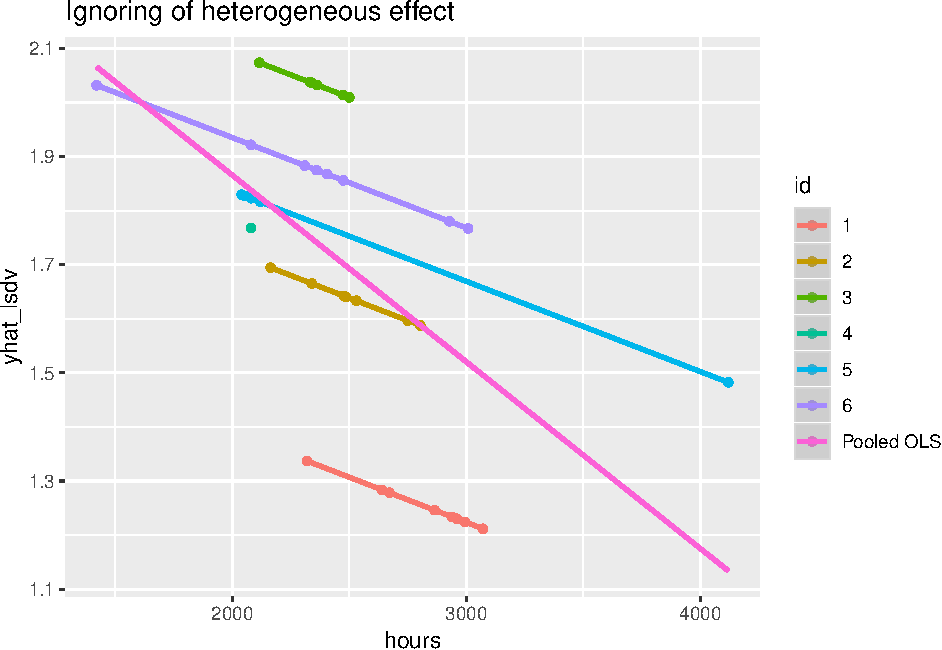
\includegraphics{09-paneldata_files/figure-latex/ignoring hetero-1.pdf}

Теперь то же самое в Stata

Для начала подгрузим данные и посмотрим на них. Сперва визуализируем малый датасет.

\begin{verbatim}
use lwage_panel_small
summarize
\end{verbatim}

\begin{verbatim}
    Variable |        Obs        Mean    Std. Dev.       Min        Max
-------------+---------------------------------------------------------
          nr |         48    364.6667    390.3276         13        910
        year |         48      1983.5    2.315535       1980       1987
       black |         48          .5    .5052912          0          1
       exper |         48    5.833333    2.636353          1         11
        hisp |         48           0           0          0          0
-------------+---------------------------------------------------------
       hours |         48    2407.875    425.1116       1420       4120
     married |         48       .1875    .3944428          0          1
        educ |         48          13     .825137         12         14
       union |         48        .125    .3342187          0          1
       lwage |         48    1.724878    .4719456  -.7202626   2.873161
-------------+---------------------------------------------------------
     expersq |         48    40.83333      31.933          1        121
  occupation |         48    4.083333    2.359529          1          9
          id |         48         3.5    1.725898          1          6
\end{verbatim}

\begin{verbatim}
xtset id year
xtline hours, overlay
clear
\end{verbatim}

\begin{verbatim}
       panel variable:  id (strongly balanced)
        time variable:  year, 1980 to 1987
                delta:  1 unit
\end{verbatim}

\begin{verbatim}
use lwage_panel_large
xtset id year
summarize
\end{verbatim}

\begin{verbatim}
       panel variable:  id (strongly balanced)
        time variable:  year, 1980 to 1987
                delta:  1 unit

    Variable |        Obs        Mean    Std. Dev.       Min        Max
-------------+---------------------------------------------------------
          nr |      4,360    5262.059     3496.15         13      12548
        year |      4,360      1983.5    2.291551       1980       1987
       black |      4,360    .1155963    .3197769          0          1
       exper |      4,360    6.514679    2.825873          0         18
        hisp |      4,360    .1559633    .3628622          0          1
-------------+---------------------------------------------------------
       hours |      4,360    2191.257    566.3523        120       4992
     married |      4,360    .4389908    .4963208          0          1
        educ |      4,360    11.76697    1.746181          3         16
       union |      4,360    .2440367    .4295639          0          1
       lwage |      4,360    1.649147    .5326094  -3.579079    4.05186
-------------+---------------------------------------------------------
     expersq |      4,360    50.42477    40.78199          0        324
  occupation |      4,360    4.988532    2.319978          1          9
          id |      4,360         273    157.3457          1        545
\end{verbatim}

Визуализируем данные. Если необходимо разнести линии на разные графики, следует убрать прараметр `overlay'.

Сгенерируем новую переменную и оценим модель с фиксированными эффектами. Последний аргумент произведёт оценку стандартных ошибок переменных в форме Хубера/Уайта

\begin{verbatim}

xtreg lwage hours, fe vce(robust)
\end{verbatim}

\begin{verbatim}
Fixed-effects (within) regression               Number of obs     =      4,360
Group variable: id                              Number of groups  =        545

R-sq:                                           Obs per group:
     within  = 0.0000                                         min =          8
     between = 0.0004                                         avg =        8.0
     overall = 0.0001                                         max =          8

                                                F(1,544)          =       0.00
corr(u_i, Xb)  = -0.0144                        Prob > F          =     0.9822

                                   (Std. Err. adjusted for 545 clusters in id)
------------------------------------------------------------------------------
             |               Robust
       lwage |      Coef.   Std. Err.      t    P>|t|     [95% Conf. Interval]
-------------+----------------------------------------------------------------
       hours |  -5.59e-07   .0000251    -0.02   0.982    -.0000498    .0000487
       _cons |   1.650371   .0549505    30.03   0.000      1.54243    1.758312
-------------+----------------------------------------------------------------
     sigma_u |  .39075125
     sigma_e |  .38728237
         rho |  .50445844   (fraction of variance due to u_i)
------------------------------------------------------------------------------
\end{verbatim}

Сделаем то же самое для модели со случайными эффектами.

\begin{verbatim}
xtreg lwage hours, re vce(robust)
\end{verbatim}

\begin{verbatim}
Random-effects GLS regression                   Number of obs     =      4,360
Group variable: id                              Number of groups  =        545

R-sq:                                           Obs per group:
     within  = 0.0000                                         min =          8
     between = 0.0004                                         avg =        8.0
     overall = 0.0001                                         max =          8

                                                Wald chi2(1)      =       0.00
corr(u_i, X)   = 0 (assumed)                    Prob > chi2       =     0.9510

                                   (Std. Err. adjusted for 545 clusters in id)
------------------------------------------------------------------------------
             |               Robust
       lwage |      Coef.   Std. Err.      z    P>|z|     [95% Conf. Interval]
-------------+----------------------------------------------------------------
       hours |   1.46e-06   .0000238     0.06   0.951    -.0000451    .0000481
       _cons |   1.645945   .0549594    29.95   0.000     1.538227    1.753664
-------------+----------------------------------------------------------------
     sigma_u |  .36626431
     sigma_e |  .38728237
         rho |   .4721295   (fraction of variance due to u_i)
------------------------------------------------------------------------------
\end{verbatim}

Тест Хаусмана.

\begin{verbatim}
xtreg lwage hours, re
estimates store b_re
xtreg lwage hours, fe
estimates store b_fe
hausman b_fe b_re, sigmamore
\end{verbatim}

\begin{verbatim}
Random-effects GLS regression                   Number of obs     =      4,360
Group variable: id                              Number of groups  =        545

R-sq:                                           Obs per group:
     within  = 0.0000                                         min =          8
     between = 0.0004                                         avg =        8.0
     overall = 0.0001                                         max =          8

                                                Wald chi2(1)      =       0.01
corr(u_i, X)   = 0 (assumed)                    Prob > chi2       =     0.9128

------------------------------------------------------------------------------
       lwage |      Coef.   Std. Err.      z    P>|z|     [95% Conf. Interval]
-------------+----------------------------------------------------------------
       hours |   1.46e-06   .0000133     0.11   0.913    -.0000247    .0000276
       _cons |   1.645945   .0337055    48.83   0.000     1.579884    1.712007
-------------+----------------------------------------------------------------
     sigma_u |  .36626431
     sigma_e |  .38728237
         rho |   .4721295   (fraction of variance due to u_i)
------------------------------------------------------------------------------



Fixed-effects (within) regression               Number of obs     =      4,360
Group variable: id                              Number of groups  =        545

R-sq:                                           Obs per group:
     within  = 0.0000                                         min =          8
     between = 0.0004                                         avg =        8.0
     overall = 0.0001                                         max =          8

                                                F(1,3814)         =       0.00
corr(u_i, Xb)  = -0.0144                        Prob > F          =     0.9682

------------------------------------------------------------------------------
       lwage |      Coef.   Std. Err.      t    P>|t|     [95% Conf. Interval]
-------------+----------------------------------------------------------------
       hours |  -5.59e-07    .000014    -0.04   0.968     -.000028    .0000269
       _cons |   1.650371   .0312611    52.79   0.000     1.589081    1.711661
-------------+----------------------------------------------------------------
     sigma_u |  .39075125
     sigma_e |  .38728237
         rho |  .50445844   (fraction of variance due to u_i)
------------------------------------------------------------------------------
F test that all u_i=0: F(544, 3814) = 8.14                   Prob > F = 0.0000

                 ---- Coefficients ----
             |      (b)          (B)            (b-B)     sqrt(diag(V_b-V_B))
             |      b_fe         b_re        Difference          S.E.
-------------+----------------------------------------------------------------
       hours |   -5.59e-07     1.46e-06       -2.02e-06        4.26e-06
------------------------------------------------------------------------------
                           b = consistent under Ho and Ha; obtained from xtreg
            B = inconsistent under Ha, efficient under Ho; obtained from xtreg

    Test:  Ho:  difference in coefficients not systematic

                  chi2(1) = (b-B)'[(V_b-V_B)^(-1)](b-B)
                          =        0.22
                Prob>chi2 =      0.6354
\end{verbatim}

Оценим FD-модель.

\begin{verbatim}
reg D.(lwage hours), vce(robust) nocon
\end{verbatim}

\begin{verbatim}
Linear regression                               Number of obs     =      3,815
                                                F(1, 3814)        =      93.15
                                                Prob > F          =     0.0000
                                                R-squared         =     0.0483
                                                Root MSE          =     .43793

------------------------------------------------------------------------------
             |               Robust
     D.lwage |      Coef.   Std. Err.      t    P>|t|     [95% Conf. Interval]
-------------+----------------------------------------------------------------
       hours |
         D1. |   -.000203    .000021    -9.65   0.000    -.0002443   -.0001618
------------------------------------------------------------------------------
\end{verbatim}

Аналогично оцениваем модель pooled OLS.

\begin{verbatim}
reg lwage hours, vce(robust)
\end{verbatim}

\begin{verbatim}
Linear regression                               Number of obs     =      4,360
                                                F(1, 4358)        =       0.27
                                                Prob > F          =     0.6059
                                                R-squared         =     0.0001
                                                Root MSE          =     .53264

------------------------------------------------------------------------------
             |               Robust
       lwage |      Coef.   Std. Err.      t    P>|t|     [95% Conf. Interval]
-------------+----------------------------------------------------------------
       hours |   9.36e-06   .0000181     0.52   0.606    -.0000262    .0000449
       _cons |   1.628646   .0415015    39.24   0.000     1.547282     1.71001
------------------------------------------------------------------------------
\end{verbatim}

Оценим LSDV-модель.

\begin{verbatim}
areg lwage hours, absorb(id)
\end{verbatim}

\begin{verbatim}
Linear regression, absorbing indicators         Number of obs     =      4,360
                                                F(   1,   3814)   =       0.00
                                                Prob > F          =     0.9682
                                                R-squared         =     0.5374
                                                Adj R-squared     =     0.4713
                                                Root MSE          =     0.3873

------------------------------------------------------------------------------
       lwage |      Coef.   Std. Err.      t    P>|t|     [95% Conf. Interval]
-------------+----------------------------------------------------------------
       hours |  -5.59e-07    .000014    -0.04   0.968     -.000028    .0000269
       _cons |   1.650371   .0312611    52.79   0.000     1.589081    1.711661
-------------+----------------------------------------------------------------
          id |      F(544, 3814) =      8.142   0.000         (545 categories)
\end{verbatim}

Повторим в Python.

\begin{Shaded}
\begin{Highlighting}[]
\ImportTok{import}\NormalTok{ numpy }\ImportTok{as}\NormalTok{ np}
\ImportTok{import}\NormalTok{ pandas }\ImportTok{as}\NormalTok{ pd}
\end{Highlighting}
\end{Shaded}

\begin{verbatim}
Error in py_call_impl(callable, dots$args, dots$keywords): ModuleNotFoundError: No module named 'pandas'

Detailed traceback: 
  File "<string>", line 1, in <module>
\end{verbatim}

Подгрузим данные и для обозначения панельных данных присвоим соответствующие индексы. Зададим соответствующие зависимые и независимые переменные, а также регрессионную формулу. Переменная ``Entity effects'' (Фиксированные эффекты) обязательна для включения для корректного распознавания панельных данных. Если её не включить, результат будет отличаться от R и STATA.

\begin{Shaded}
\begin{Highlighting}[]
\NormalTok{df }\OperatorTok{=}\NormalTok{ pd.read_csv(}\StringTok{"lwage_panel_large.csv"}\NormalTok{)}
\end{Highlighting}
\end{Shaded}

\begin{verbatim}
Error in py_call_impl(callable, dots$args, dots$keywords): NameError: name 'pd' is not defined

Detailed traceback: 
  File "<string>", line 1, in <module>
\end{verbatim}

\begin{Shaded}
\begin{Highlighting}[]
\NormalTok{df }\OperatorTok{=}\NormalTok{ df.set_index([}\StringTok{'id'}\NormalTok{, }\StringTok{'year'}\NormalTok{])}
\end{Highlighting}
\end{Shaded}

\begin{verbatim}
Error in py_call_impl(callable, dots$args, dots$keywords): NameError: name 'df' is not defined

Detailed traceback: 
  File "<string>", line 1, in <module>
\end{verbatim}

\begin{Shaded}
\begin{Highlighting}[]
\NormalTok{formula }\OperatorTok{=} \StringTok{'lwage ~ 1 + hours + EntityEffects'}
\NormalTok{dependent }\OperatorTok{=}\NormalTok{ df.lwage}
\end{Highlighting}
\end{Shaded}

\begin{verbatim}
Error in py_call_impl(callable, dots$args, dots$keywords): NameError: name 'df' is not defined

Detailed traceback: 
  File "<string>", line 1, in <module>
\end{verbatim}

\begin{Shaded}
\begin{Highlighting}[]
\NormalTok{regressors }\OperatorTok{=}\NormalTok{ df[[}\StringTok{'hours'}\NormalTok{]]}
\end{Highlighting}
\end{Shaded}

\begin{verbatim}
Error in py_call_impl(callable, dots$args, dots$keywords): NameError: name 'df' is not defined

Detailed traceback: 
  File "<string>", line 1, in <module>
\end{verbatim}

\begin{Shaded}
\begin{Highlighting}[]
\BuiltInTok{print}\NormalTok{(df.head())}
\end{Highlighting}
\end{Shaded}

\begin{verbatim}
Error in py_call_impl(callable, dots$args, dots$keywords): NameError: name 'df' is not defined

Detailed traceback: 
  File "<string>", line 1, in <module>
\end{verbatim}

Оценим FE-модель, используя within-оценку.

\begin{Shaded}
\begin{Highlighting}[]
\ImportTok{from}\NormalTok{ linearmodels }\ImportTok{import}\NormalTok{ PanelOLS}
\end{Highlighting}
\end{Shaded}

\begin{verbatim}
Error in py_call_impl(callable, dots$args, dots$keywords): ModuleNotFoundError: No module named 'linearmodels'

Detailed traceback: 
  File "<string>", line 1, in <module>
\end{verbatim}

\begin{Shaded}
\begin{Highlighting}[]
\NormalTok{model_fe }\OperatorTok{=}\NormalTok{ PanelOLS.from_formula(formula, df)}
\end{Highlighting}
\end{Shaded}

\begin{verbatim}
Error in py_call_impl(callable, dots$args, dots$keywords): NameError: name 'PanelOLS' is not defined

Detailed traceback: 
  File "<string>", line 1, in <module>
\end{verbatim}

\begin{Shaded}
\begin{Highlighting}[]
\NormalTok{model_fe_fitted }\OperatorTok{=}\NormalTok{ model_fe.fit(cov_type}\OperatorTok{=}\StringTok{'clustered'}\NormalTok{, cluster_entity }\OperatorTok{=} \VariableTok{True}\NormalTok{)}
\end{Highlighting}
\end{Shaded}

\begin{verbatim}
Error in py_call_impl(callable, dots$args, dots$keywords): NameError: name 'model_fe' is not defined

Detailed traceback: 
  File "<string>", line 1, in <module>
\end{verbatim}

\begin{Shaded}
\begin{Highlighting}[]
\BuiltInTok{print}\NormalTok{(model_fe_fitted)}
\end{Highlighting}
\end{Shaded}

\begin{verbatim}
Error in py_call_impl(callable, dots$args, dots$keywords): NameError: name 'model_fe_fitted' is not defined

Detailed traceback: 
  File "<string>", line 1, in <module>
\end{verbatim}

Оценим RE-модель, используя FGLS-оценку.

\begin{Shaded}
\begin{Highlighting}[]
\ImportTok{from}\NormalTok{ linearmodels.panel }\ImportTok{import}\NormalTok{ RandomEffects}
\end{Highlighting}
\end{Shaded}

\begin{verbatim}
Error in py_call_impl(callable, dots$args, dots$keywords): ModuleNotFoundError: No module named 'linearmodels'

Detailed traceback: 
  File "<string>", line 1, in <module>
\end{verbatim}

\begin{Shaded}
\begin{Highlighting}[]
\NormalTok{model_re }\OperatorTok{=}\NormalTok{ RandomEffects.from_formula(formula, df)}
\end{Highlighting}
\end{Shaded}

\begin{verbatim}
Error in py_call_impl(callable, dots$args, dots$keywords): NameError: name 'RandomEffects' is not defined

Detailed traceback: 
  File "<string>", line 1, in <module>
\end{verbatim}

\begin{Shaded}
\begin{Highlighting}[]
\NormalTok{model_re_fitted }\OperatorTok{=}\NormalTok{ model_re.fit(cov_type}\OperatorTok{=}\StringTok{'clustered'}\NormalTok{, cluster_entity }\OperatorTok{=} \VariableTok{True}\NormalTok{)}
\end{Highlighting}
\end{Shaded}

\begin{verbatim}
Error in py_call_impl(callable, dots$args, dots$keywords): NameError: name 'model_re' is not defined

Detailed traceback: 
  File "<string>", line 1, in <module>
\end{verbatim}

\begin{Shaded}
\begin{Highlighting}[]
\BuiltInTok{dir}\NormalTok{(model_re_fitted)}
\end{Highlighting}
\end{Shaded}

\begin{verbatim}
Error in py_call_impl(callable, dots$args, dots$keywords): NameError: name 'model_re_fitted' is not defined

Detailed traceback: 
  File "<string>", line 1, in <module>
\end{verbatim}

\begin{Shaded}
\begin{Highlighting}[]
\BuiltInTok{print}\NormalTok{(model_re_fitted)}
\end{Highlighting}
\end{Shaded}

\begin{verbatim}
Error in py_call_impl(callable, dots$args, dots$keywords): NameError: name 'model_re_fitted' is not defined

Detailed traceback: 
  File "<string>", line 1, in <module>
\end{verbatim}

Тест Хаусмана в соответствующем пакете на данный момент не реализован.

Оценим модель Pooled OLS

\begin{Shaded}
\begin{Highlighting}[]
\ImportTok{from}\NormalTok{ linearmodels.panel }\ImportTok{import}\NormalTok{ PooledOLS}
\end{Highlighting}
\end{Shaded}

\begin{verbatim}
Error in py_call_impl(callable, dots$args, dots$keywords): ModuleNotFoundError: No module named 'linearmodels'

Detailed traceback: 
  File "<string>", line 1, in <module>
\end{verbatim}

\begin{Shaded}
\begin{Highlighting}[]
\NormalTok{model_pool }\OperatorTok{=}\NormalTok{ PooledOLS.from_formula(formula, df)}
\end{Highlighting}
\end{Shaded}

\begin{verbatim}
Error in py_call_impl(callable, dots$args, dots$keywords): NameError: name 'PooledOLS' is not defined

Detailed traceback: 
  File "<string>", line 1, in <module>
\end{verbatim}

\begin{Shaded}
\begin{Highlighting}[]
\NormalTok{model_pool_fitted }\OperatorTok{=}\NormalTok{ model_pool.fit(cov_type}\OperatorTok{=}\StringTok{'clustered'}\NormalTok{, cluster_entity }\OperatorTok{=} \VariableTok{True}\NormalTok{)}
\end{Highlighting}
\end{Shaded}

\begin{verbatim}
Error in py_call_impl(callable, dots$args, dots$keywords): NameError: name 'model_pool' is not defined

Detailed traceback: 
  File "<string>", line 1, in <module>
\end{verbatim}

\begin{Shaded}
\begin{Highlighting}[]
\BuiltInTok{print}\NormalTok{(model_pool_fitted)}
\end{Highlighting}
\end{Shaded}

\begin{verbatim}
Error in py_call_impl(callable, dots$args, dots$keywords): NameError: name 'model_pool_fitted' is not defined

Detailed traceback: 
  File "<string>", line 1, in <module>
\end{verbatim}

Оценим LSDV-модель

\begin{Shaded}
\begin{Highlighting}[]
\NormalTok{model_lsdv }\OperatorTok{=}\NormalTok{ PanelOLS.from_formula(formula, df)}
\NormalTok{model_lsdv_fitted }\OperatorTok{=}\NormalTok{ model_lsdv.fit(cov_type}\OperatorTok{=}\StringTok{'clustered'}\NormalTok{, cluster_entity }\OperatorTok{=} \VariableTok{True}\NormalTok{, use_lsdv }\OperatorTok{=} \VariableTok{True}\NormalTok{)}
\BuiltInTok{print}\NormalTok{(model_lsdv_fitted)}
\end{Highlighting}
\end{Shaded}

Построим FD-оценку. Здесь необходимо убрать константный признак, так как данная модель начинает выдавать ошибку. Логически, конечно, он автоматически должен исчезнуть по построению модели, но в данной реализации это требуется задать на уровне пользователя.

\begin{Shaded}
\begin{Highlighting}[]
\ImportTok{from}\NormalTok{ linearmodels.panel }\ImportTok{import}\NormalTok{ FirstDifferenceOLS}
\end{Highlighting}
\end{Shaded}

\begin{verbatim}
Error in py_call_impl(callable, dots$args, dots$keywords): ModuleNotFoundError: No module named 'linearmodels'

Detailed traceback: 
  File "<string>", line 1, in <module>
\end{verbatim}

\begin{Shaded}
\begin{Highlighting}[]
\NormalTok{formula_fd }\OperatorTok{=} \StringTok{'lwage ~ hours + EntityEffects'}
\NormalTok{model_fd }\OperatorTok{=}\NormalTok{ FirstDifferenceOLS.from_formula(formula_fd, df)}
\end{Highlighting}
\end{Shaded}

\begin{verbatim}
Error in py_call_impl(callable, dots$args, dots$keywords): NameError: name 'FirstDifferenceOLS' is not defined

Detailed traceback: 
  File "<string>", line 1, in <module>
\end{verbatim}

\begin{Shaded}
\begin{Highlighting}[]
\NormalTok{model_fd_fitted }\OperatorTok{=}\NormalTok{ model_fd.fit(cov_type}\OperatorTok{=}\StringTok{'clustered'}\NormalTok{, cluster_entity }\OperatorTok{=} \VariableTok{True}\NormalTok{)}
\end{Highlighting}
\end{Shaded}

\begin{verbatim}
Error in py_call_impl(callable, dots$args, dots$keywords): NameError: name 'model_fd' is not defined

Detailed traceback: 
  File "<string>", line 1, in <module>
\end{verbatim}

\begin{Shaded}
\begin{Highlighting}[]
\BuiltInTok{print}\NormalTok{(model_fd_fitted)}
\end{Highlighting}
\end{Shaded}

\begin{verbatim}
Error in py_call_impl(callable, dots$args, dots$keywords): NameError: name 'model_fd_fitted' is not defined

Detailed traceback: 
  File "<string>", line 1, in <module>
\end{verbatim}

\hypertarget{heterosked}{%
\chapter{Гетероскедастичность в простой регрессии}\label{heterosked}}

\begin{quote}
Одним из нарушений условий ТГМ является гетероскедастичность, возникающая ввиду неодинаковых дисперсий для разных наблюдений. Она нежелательна ввиду того, что оценки МНК не являются эффективными (но остаются несмещёнными), и предпосылки для использования \texttt{t}-статистик нарушены, что даёт неверный результат о значимости коэффициентов.
\end{quote}

Этот коан благословит Вас на поиски гетероскедастичности и просветит о способах борьбы с ней.

Будем анализировать гетероскедастичность на данных о стоимости квартир.

\hypertarget{r-3}{%
\section{r}\label{r-3}}

Вызовем \textbf{r} в помощь в охоте на гетероскедастичность. Импортируем его оружейные пакеты.

\begin{Shaded}
\begin{Highlighting}[]
\KeywordTok{library}\NormalTok{(rio) }\CommentTok{# импорт и экспорт данных в разных форматах}
\KeywordTok{library}\NormalTok{(dplyr) }\CommentTok{# манипуляции с данными}
\KeywordTok{library}\NormalTok{(lmtest) }\CommentTok{# тест Бройша-Пагана}
\KeywordTok{library}\NormalTok{(sandwich) }\CommentTok{# оценка дисперсии при гетероскедастичности}
\KeywordTok{library}\NormalTok{(UStatBookABSC) }\CommentTok{# WLS}
\end{Highlighting}
\end{Shaded}

\begin{verbatim}
Error in library(UStatBookABSC): there is no package called 'UStatBookABSC'
\end{verbatim}

\begin{Shaded}
\begin{Highlighting}[]
\KeywordTok{library}\NormalTok{ (estimatr) }\CommentTok{# получение робастных оценок}
\KeywordTok{library}\NormalTok{(ggpubr) }\CommentTok{# для графиков}
\KeywordTok{library}\NormalTok{(skimr) }\CommentTok{# для описательных статистик}
\end{Highlighting}
\end{Shaded}

Импортируем наш dataset, \texttt{flats.dta}:

\begin{Shaded}
\begin{Highlighting}[]
\NormalTok{flats=}\StringTok{ }\KeywordTok{import}\NormalTok{(}\StringTok{"data/flats.dta"}\NormalTok{)}
\end{Highlighting}
\end{Shaded}

\begin{verbatim}
Error in import("data/flats.dta"): No such file
\end{verbatim}

Рассмотрим описательные статистики загруженного датасета.

\begin{Shaded}
\begin{Highlighting}[]
\KeywordTok{skim}\NormalTok{(flats)}
\end{Highlighting}
\end{Shaded}

\begin{verbatim}
Error in skim(flats): object 'flats' not found
\end{verbatim}

Построим простую линейную регрессионную модель, на которой будем проверять гетероскедастичность.

\begin{Shaded}
\begin{Highlighting}[]
\NormalTok{reg =}\StringTok{ }\KeywordTok{lm}\NormalTok{(ln_price_metr }\OperatorTok{~}\StringTok{ }\DecValTok{1} \OperatorTok{+}\StringTok{ }\NormalTok{ln_livesp }\OperatorTok{+}\StringTok{ }\NormalTok{ln_kitsp }\OperatorTok{+}\StringTok{ }\NormalTok{ln_dist }\OperatorTok{+}\StringTok{ }\NormalTok{ln_metrdist, }\DataTypeTok{data=}\NormalTok{flats)}
\end{Highlighting}
\end{Shaded}

\begin{verbatim}
Error in is.data.frame(data): object 'flats' not found
\end{verbatim}

\begin{Shaded}
\begin{Highlighting}[]
\KeywordTok{summary}\NormalTok{(reg)}
\end{Highlighting}
\end{Shaded}

\begin{verbatim}
Error in summary(reg): object 'reg' not found
\end{verbatim}

Проверим наличие гетероскедастичности визуально. Построим зависимости цены квартир от объясняющих факторов.

\begin{Shaded}
\begin{Highlighting}[]
\NormalTok{kit =}\StringTok{ }\KeywordTok{ggplot}\NormalTok{(flats) }\OperatorTok{+}\StringTok{ }\KeywordTok{geom_point}\NormalTok{(}\KeywordTok{aes}\NormalTok{(}\DataTypeTok{x =}\NormalTok{ ln_kitsp, }\DataTypeTok{y =}\NormalTok{ ln_price_metr)) }\OperatorTok{+}\StringTok{ }
\StringTok{  }\KeywordTok{labs}\NormalTok{(}\DataTypeTok{x =} \StringTok{"Площадь кухни, кв.м"}\NormalTok{, }\DataTypeTok{y =} \StringTok{"Цена квартиры, $1000"}\NormalTok{, }
  \DataTypeTok{title =} \StringTok{"Стоимость квартир в Москве"}\NormalTok{)}
\end{Highlighting}
\end{Shaded}

\begin{verbatim}
Error in ggplot(flats): object 'flats' not found
\end{verbatim}

\begin{Shaded}
\begin{Highlighting}[]
\NormalTok{live =}\StringTok{ }\KeywordTok{ggplot}\NormalTok{(flats) }\OperatorTok{+}\StringTok{ }\KeywordTok{geom_point}\NormalTok{(}\KeywordTok{aes}\NormalTok{(}\DataTypeTok{x =}\NormalTok{ ln_livesp, }\DataTypeTok{y =}\NormalTok{ ln_price_metr)) }\OperatorTok{+}\StringTok{ }
\StringTok{  }\KeywordTok{labs}\NormalTok{(}\DataTypeTok{x =} \StringTok{"Жилая площадь, кв.м"}\NormalTok{, }\DataTypeTok{y =} \StringTok{"Цена квартиры, $1000"}\NormalTok{, }
  \DataTypeTok{title =} \StringTok{"Стоимость квартир в Москве"}\NormalTok{)}
\end{Highlighting}
\end{Shaded}

\begin{verbatim}
Error in ggplot(flats): object 'flats' not found
\end{verbatim}

\begin{Shaded}
\begin{Highlighting}[]
\NormalTok{dist =}\StringTok{ }\KeywordTok{ggplot}\NormalTok{(flats) }\OperatorTok{+}\StringTok{ }\KeywordTok{geom_point}\NormalTok{(}\KeywordTok{aes}\NormalTok{(}\DataTypeTok{x =}\NormalTok{ ln_dist, }\DataTypeTok{y =}\NormalTok{ ln_price_metr)) }\OperatorTok{+}\StringTok{ }
\StringTok{  }\KeywordTok{labs}\NormalTok{(}\DataTypeTok{x =} \StringTok{"Расстояние до центра, м"}\NormalTok{, }\DataTypeTok{y =} \StringTok{"Цена квартиры, $1000"}\NormalTok{,}
  \DataTypeTok{title =} \StringTok{"Стоимость квартир в Москве"}\NormalTok{)}
\end{Highlighting}
\end{Shaded}

\begin{verbatim}
Error in ggplot(flats): object 'flats' not found
\end{verbatim}

\begin{Shaded}
\begin{Highlighting}[]
\NormalTok{metrdist =}\StringTok{ }\KeywordTok{ggplot}\NormalTok{(flats) }\OperatorTok{+}\StringTok{ }\KeywordTok{geom_point}\NormalTok{(}\KeywordTok{aes}\NormalTok{(}\DataTypeTok{x =}\NormalTok{ ln_metrdist, }\DataTypeTok{y =}\NormalTok{ ln_price_metr)) }\OperatorTok{+}\StringTok{ }
\StringTok{  }\KeywordTok{labs}\NormalTok{(}\DataTypeTok{x =} \StringTok{"Расстояние до метро, м"}\NormalTok{, }\DataTypeTok{y =} \StringTok{"Цена квартиры, $1000"}\NormalTok{, }
  \DataTypeTok{title =} \StringTok{"Стоимость квартир в Москве"}\NormalTok{)}
\end{Highlighting}
\end{Shaded}

\begin{verbatim}
Error in ggplot(flats): object 'flats' not found
\end{verbatim}

\begin{Shaded}
\begin{Highlighting}[]
\KeywordTok{ggarrange}\NormalTok{(kit, live, dist, metrdist, }\DataTypeTok{ncol=}\DecValTok{2}\NormalTok{, }\DataTypeTok{nrow=}\DecValTok{2}\NormalTok{)}
\end{Highlighting}
\end{Shaded}

\begin{verbatim}
Error in ggarrange(kit, live, dist, metrdist, ncol = 2, nrow = 2): object 'kit' not found
\end{verbatim}

Из сета красивых графиков видно, что гетероскедастичность присутствует. В частности, подозрительны переменные \texttt{ln\_kitsp} и \texttt{ln\_metrdist}.

Проверим наличие гетероскедастичности с помощью тестов. Начнём с теста Уайта. Он неконструктивный, он может лишь показать наличие гетероскедастичности, асимптотический. Нормальность остатков в предпосылках не требуется, подразумевается, что \[E{\varepsilon^4_i} = const\].

\[
\begin{cases}
H_0: \sigma^2_i = \sigma^2 \\
H_1: \sigma^2_i \neq = \sigma^2 \\
\end{cases}
\]

На первом шаге тест сохраняет остатки от построения начальной регрессии.
\[
\hat{\ln{(pricemetr_i)}} = \hat{\beta}_0 + \hat{\beta}_{\ln{(kitsp)}} \cdot \ln{(kitsp_i)} + \hat{\beta}_{\ln{(livesp)}}\cdot \ln{(livesp_i)} + \hat{\beta}_{\ln{(dist)}}\cdot \ln{(dist_i)} + \hat{\beta}_{\ln{(metrdist)}}\cdot \ln{(metrdist_i)}
\]
На втором - строится вспомогательная регрессия (X\_j-вектор j-го фактора).
\[
\hat{e}^2_i = \hat{\alpha}_0 + \sum_{j=1}^{k} \hat{\alpha}_j \cdot X_j + \sum_{j=1}^{k} \hat{\gamma}_j \cdot X^2_j + \sum_{j < m}^{k} \hat{\delta}_j X_j \cdot X_m
\]

\texttt{R-squared} построенной вспомогательной регрессии должен быть распределён как:
\[
n \cdot R^2_{aux} \sim \chi^2_{K-1}
\]
где \texttt{K} -- число факторов во вспомогательной регрессии.

Тест Уайта реализуется (ручками) как:

\begin{Shaded}
\begin{Highlighting}[]
\KeywordTok{bptest}\NormalTok{(reg, }\DataTypeTok{varformula =} \OperatorTok{~}\StringTok{ }\DecValTok{1} \OperatorTok{+}\StringTok{ }\NormalTok{ln_livesp }\OperatorTok{+}\StringTok{ }\NormalTok{ln_kitsp }\OperatorTok{+}\StringTok{ }\NormalTok{ln_dist }\OperatorTok{+}\StringTok{ }\NormalTok{ln_metrdist }\OperatorTok{+}\StringTok{ }\KeywordTok{I}\NormalTok{(ln_livesp }\OperatorTok{^}\StringTok{ }\DecValTok{2}\NormalTok{) }\OperatorTok{+}\StringTok{ }\KeywordTok{I}\NormalTok{(ln_kitsp }\OperatorTok{^}\StringTok{ }\DecValTok{2}\NormalTok{) }\OperatorTok{+}\StringTok{ }\KeywordTok{I}\NormalTok{(ln_dist }\OperatorTok{^}\StringTok{ }\DecValTok{2}\NormalTok{) }\OperatorTok{+}\StringTok{ }\KeywordTok{I}\NormalTok{(ln_metrdist }\OperatorTok{^}\StringTok{ }\DecValTok{2}\NormalTok{) }\OperatorTok{+}\StringTok{ }\KeywordTok{I}\NormalTok{(ln_livesp }\OperatorTok{*}\StringTok{ }\NormalTok{ln_kitsp) }\OperatorTok{+}\StringTok{ }\KeywordTok{I}\NormalTok{(ln_livesp }\OperatorTok{*}\StringTok{ }\NormalTok{ln_dist) }\OperatorTok{+}\StringTok{ }\KeywordTok{I}\NormalTok{(ln_livesp }\OperatorTok{*}\StringTok{ }\NormalTok{ln_metrdist) }\OperatorTok{+}\StringTok{ }\KeywordTok{I}\NormalTok{(ln_kitsp }\OperatorTok{*}\StringTok{ }\NormalTok{ln_dist) }\OperatorTok{+}\StringTok{ }\KeywordTok{I}\NormalTok{(ln_kitsp }\OperatorTok{*}\StringTok{ }\NormalTok{ln_metrdist) }\OperatorTok{+}\StringTok{ }\KeywordTok{I}\NormalTok{(ln_dist }\OperatorTok{*}\StringTok{ }\NormalTok{ln_metrdist), }\DataTypeTok{data=}\NormalTok{flats)}
\end{Highlighting}
\end{Shaded}

\begin{verbatim}
Error in bptest(reg, varformula = ~1 + ln_livesp + ln_kitsp + ln_dist + : object 'reg' not found
\end{verbatim}

Тест Уайта выявил гетероскедастичность.

Тест Бройша-Пагана -- обобщённый вариант теста Уайта. В тесте Бройша-Пагана во вспомогательной регрессии можно брать любые функции от регрессоров, в тесте Уайта - регрессоры, их квадраты и кросс-произведения. Тест Бройша-Пагана является асимптотическим.

\[
\begin{cases}
H_0: \sigma^2_i = \sigma^2 \\
H_1: \sigma^2_i \propto f(\alpha_0 + \alpha_1 \cdot Z_1 +  \ldots + \alpha_p \cdot Z_p) \\
\end{cases}
\]

Классическая версия Бройша-Пагана строится на основе метода максимального правдоподобия. Предпосылками классической версии теста являются нормальность остатков, существование у функции дисперсии из альтернативной гипотезы первой и второй производной. Считается LM-статистика, которая, при верной основной гипотезе об отсутствии гетероскедастичности, имеет хи-квадратное распределение с p-1 степенью свободы.

Классическая версия Бройша-Пагана реализуется в \textbf{r} по команде:

\begin{Shaded}
\begin{Highlighting}[]
\KeywordTok{bptest}\NormalTok{(reg, }\DataTypeTok{studentize=}\OtherTok{FALSE}\NormalTok{)}
\end{Highlighting}
\end{Shaded}

\begin{verbatim}
Error in bptest(reg, studentize = FALSE): object 'reg' not found
\end{verbatim}

Современная модификация теста не требует нормальности остатков, лишь \[{\mathbb E}({\varepsilon^4_i}) = const\].
На первом шаге строится исходная регрессия и сохраняются остатки. Затем строится состоятельная оценка дисперсии:
\[
\hat{\sigma}^2 = \frac{1}{n} \cdot \sum_{i=1}^{n} {e^2_i}
\]
Потом строится вспомогательная регрессия:
\[
\frac{e^2}{\hat{\sigma}^2} = \alpha_0 + \alpha_1 \cdot Z_1 + \ldots + \alpha_p \cdot Z_p + u
\]
И рассчитывается тестовая статистика:
\[
\frac{RSS_{aux}}{2} \sim \chi^2_{p}
\]
Модифицированная версия теста Бройша-Пагана реализуется по команде:

\begin{Shaded}
\begin{Highlighting}[]
\KeywordTok{bptest}\NormalTok{(reg)}
\end{Highlighting}
\end{Shaded}

\begin{verbatim}
Error in bptest(reg): object 'reg' not found
\end{verbatim}

Причем, если отдельно не указать спецификацию вспомогательной регрессии, то \texttt{bptest()} возьмёт все регрессоры исходной модели.

В обеих версиях теста Бройша-Пагана гетероскедастичность обнаружена.

Ещё есть тест Голдфелда-Квандта.

\[
\begin{cases}
H_0: \sigma^2_i = \sigma^2 \\
H_1: \sigma^2_i \propto X_i \\
\end{cases}
\]

Этот тест предполагает нормальность остатков и является неасимптотическим.

Процедура:

Сначала все наблюдения сортируются по возрастанию абсолютного значения фактора, вызывающего гетероскедастичность.

Затем отсортированный ряд по фактору делится на 3 примерно равные части. Считаются гетероскедастичности по первой и третьей части ряда.
Строится \texttt{F}-статистика:
\[
\frac{RSS_2}{RSS_1} \sim F_{r - k, r-k}
\]

где \texttt{r} - размер первой и третьей частей отсортированного ряда.

Данный тест в \textbf{r} реализуется по командам (предполагается, что дисперсии пропорциональны переменной \texttt{ln\_kitsp}):

\begin{Shaded}
\begin{Highlighting}[]
\NormalTok{flats_ordered =}\StringTok{ }\NormalTok{flats[}\KeywordTok{order}\NormalTok{(flats}\OperatorTok{$}\NormalTok{ln_kitsp), ]}
\end{Highlighting}
\end{Shaded}

\begin{verbatim}
Error in eval(expr, envir, enclos): object 'flats' not found
\end{verbatim}

\begin{Shaded}
\begin{Highlighting}[]
\NormalTok{reg_gqtest =}\StringTok{ }\KeywordTok{lm}\NormalTok{(ln_price_metr }\OperatorTok{~}\StringTok{ }\DecValTok{1} \OperatorTok{+}\StringTok{ }\NormalTok{ln_livesp }\OperatorTok{+}\StringTok{ }\NormalTok{ln_kitsp }\OperatorTok{+}\StringTok{ }\NormalTok{ln_dist }\OperatorTok{+}\StringTok{ }\NormalTok{ln_metrdist, }\DataTypeTok{data=}\NormalTok{flats_ordered)}
\end{Highlighting}
\end{Shaded}

\begin{verbatim}
Error in is.data.frame(data): object 'flats_ordered' not found
\end{verbatim}

\begin{Shaded}
\begin{Highlighting}[]
\KeywordTok{gqtest}\NormalTok{(reg_gqtest, }\DataTypeTok{fraction=}\FloatTok{0.34}\NormalTok{) }\CommentTok{# посередине отсортированного ряда лежит 34% наблюдений}
\end{Highlighting}
\end{Shaded}

\begin{verbatim}
Error in gqtest(reg_gqtest, fraction = 0.34): object 'reg_gqtest' not found
\end{verbatim}

Будет также полезным познакомиться с методами борьбы с гетероскедастичностью.

Способ 1. Взвешенный МНК. Веса -- оценка обратной дисперсии переменной, вызывающей гетероскедачность.
То есть оценим регрессию:
\[
\frac{\ln{(pricemetr_i)}}{\hat{\sigma}_i} = 
\frac{\beta_0}{\hat{\sigma}_i} + 
\frac{\beta_{\ln{(kitsp)}} \cdot \ln{(kitsp_i)}}{\hat{\sigma}_i} + \frac{\beta_{\ln{(livesp)}} \cdot \ln{(livesp_i)}}{\hat{\sigma}_i} + \frac{\beta_{\ln{(dist)}} \cdot \ln{(dist_i)}}{\hat{\sigma}_i} + \frac{\beta_{\ln{(metrdist)}} \cdot \ln{(metrdist_i)}}{\hat{\sigma}_i} + \frac{\varepsilon_i}{\hat{\sigma}_i}
\]

В \textbf{r} это можно сделать так:

\begin{Shaded}
\begin{Highlighting}[]
\NormalTok{reg_wls =}\StringTok{ }\KeywordTok{lm}\NormalTok{(ln_price_metr }\OperatorTok{~}\StringTok{ }\DecValTok{1} \OperatorTok{+}\StringTok{ }\NormalTok{ln_livesp }\OperatorTok{+}\StringTok{ }\NormalTok{ln_kitsp }\OperatorTok{+}\StringTok{ }\NormalTok{ln_dist }\OperatorTok{+}\StringTok{ }\NormalTok{ln_metrdist, }\DataTypeTok{data=}\NormalTok{flats, }\DataTypeTok{weights =} \DecValTok{1} \OperatorTok{/}\StringTok{ }\NormalTok{(}\DecValTok{1} \OperatorTok{/}\StringTok{ }\KeywordTok{fitted}\NormalTok{(}\KeywordTok{lm}\NormalTok{(}\KeywordTok{abs}\NormalTok{(}\KeywordTok{residuals}\NormalTok{(reg)) }\OperatorTok{~}\StringTok{ }\NormalTok{ln_kitsp)) }\OperatorTok{^}\StringTok{ }\DecValTok{2}\NormalTok{))}
\end{Highlighting}
\end{Shaded}

\begin{verbatim}
Error in is.data.frame(data): object 'flats' not found
\end{verbatim}

\begin{Shaded}
\begin{Highlighting}[]
\KeywordTok{summary}\NormalTok{(reg_wls)}
\end{Highlighting}
\end{Shaded}

\begin{verbatim}
Error in summary(reg_wls): object 'reg_wls' not found
\end{verbatim}

Способ 2. Робастные оценки Уайта.

\begin{Shaded}
\begin{Highlighting}[]
\KeywordTok{coeftest}\NormalTok{(reg, }\DataTypeTok{vcov =} \KeywordTok{vcovHC}\NormalTok{(reg, }\StringTok{"HC0"}\NormalTok{))}
\end{Highlighting}
\end{Shaded}

\begin{verbatim}
Error in coeftest(reg, vcov = vcovHC(reg, "HC0")): object 'reg' not found
\end{verbatim}

Робастные оценки коэффициентов регрессии получаются состоятельными.

\hypertarget{python-3}{%
\section{python}\label{python-3}}

Теперь попробуем проделать эти шаги в \textbf{python}.

Импотируем необходимые пакеты.

\begin{Shaded}
\begin{Highlighting}[]
\ImportTok{import}\NormalTok{ numpy }\ImportTok{as}\NormalTok{ np}
\ImportTok{import}\NormalTok{ pandas }\ImportTok{as}\NormalTok{ pd }\CommentTok{# чтение файлов}
\end{Highlighting}
\end{Shaded}

\begin{verbatim}
Error in py_call_impl(callable, dots$args, dots$keywords): ModuleNotFoundError: No module named 'pandas'

Detailed traceback: 
  File "<string>", line 1, in <module>
\end{verbatim}

\begin{Shaded}
\begin{Highlighting}[]
\ImportTok{import}\NormalTok{ matplotlib.pyplot }\ImportTok{as}\NormalTok{ plt }\CommentTok{# построение графиков}
\end{Highlighting}
\end{Shaded}

\begin{verbatim}
Error in py_call_impl(callable, dots$args, dots$keywords): ModuleNotFoundError: No module named 'matplotlib'

Detailed traceback: 
  File "<string>", line 1, in <module>
\end{verbatim}

\begin{Shaded}
\begin{Highlighting}[]
\ImportTok{import}\NormalTok{ seaborn }\ImportTok{as}\NormalTok{ sns }\CommentTok{# построение графиков}
\end{Highlighting}
\end{Shaded}

\begin{verbatim}
Error in py_call_impl(callable, dots$args, dots$keywords): ModuleNotFoundError: No module named 'seaborn'

Detailed traceback: 
  File "<string>", line 1, in <module>
\end{verbatim}

\begin{Shaded}
\begin{Highlighting}[]
\ImportTok{import}\NormalTok{ statsmodels.api }\ImportTok{as}\NormalTok{ sm }\CommentTok{# тесты}
\end{Highlighting}
\end{Shaded}

\begin{verbatim}
Error in py_call_impl(callable, dots$args, dots$keywords): ModuleNotFoundError: No module named 'statsmodels'

Detailed traceback: 
  File "<string>", line 1, in <module>
\end{verbatim}

\begin{Shaded}
\begin{Highlighting}[]
\ImportTok{from}\NormalTok{ statsmodels.formula.api }\ImportTok{import}\NormalTok{ ols, WLS }\CommentTok{# построение регрессии}
\end{Highlighting}
\end{Shaded}

\begin{verbatim}
Error in py_call_impl(callable, dots$args, dots$keywords): ModuleNotFoundError: No module named 'statsmodels'

Detailed traceback: 
  File "<string>", line 1, in <module>
\end{verbatim}

\begin{Shaded}
\begin{Highlighting}[]
\ImportTok{import}\NormalTok{ statsmodels}
\end{Highlighting}
\end{Shaded}

\begin{verbatim}
Error in py_call_impl(callable, dots$args, dots$keywords): ModuleNotFoundError: No module named 'statsmodels'

Detailed traceback: 
  File "<string>", line 1, in <module>
\end{verbatim}

\begin{Shaded}
\begin{Highlighting}[]
\ImportTok{import}\NormalTok{ statsmodels.stats.diagnostic }\ImportTok{as}\NormalTok{ sm_diagnostic }\CommentTok{# тест Бройша-Пагана}
\end{Highlighting}
\end{Shaded}

\begin{verbatim}
Error in py_call_impl(callable, dots$args, dots$keywords): ModuleNotFoundError: No module named 'statsmodels'

Detailed traceback: 
  File "<string>", line 1, in <module>
\end{verbatim}

Загрузим исследуемый датасет.

\begin{Shaded}
\begin{Highlighting}[]
\NormalTok{flats }\OperatorTok{=}\NormalTok{ pd.read_stata(}\StringTok{"data/flats.dta"}\NormalTok{)}
\end{Highlighting}
\end{Shaded}

\begin{verbatim}
Error in py_call_impl(callable, dots$args, dots$keywords): NameError: name 'pd' is not defined

Detailed traceback: 
  File "<string>", line 1, in <module>
\end{verbatim}

Построим линейную регрессионную модель.

\begin{Shaded}
\begin{Highlighting}[]
\NormalTok{reg }\OperatorTok{=}\NormalTok{ ols(}\StringTok{"ln_price_metr ~ 1 + ln_livesp + ln_kitsp + ln_dist + ln_metrdist"}\NormalTok{, flats).fit()}
\end{Highlighting}
\end{Shaded}

\begin{verbatim}
Error in py_call_impl(callable, dots$args, dots$keywords): NameError: name 'ols' is not defined

Detailed traceback: 
  File "<string>", line 1, in <module>
\end{verbatim}

\begin{Shaded}
\begin{Highlighting}[]
\NormalTok{reg.summary()}
\end{Highlighting}
\end{Shaded}

\begin{verbatim}
Error in py_call_impl(callable, dots$args, dots$keywords): NameError: name 'reg' is not defined

Detailed traceback: 
  File "<string>", line 1, in <module>
\end{verbatim}

Визуализируем зависимости регрессоров и регрессанта.

\begin{Shaded}
\begin{Highlighting}[]
\NormalTok{sns.pairplot(flats, x_vars}\OperatorTok{=}\NormalTok{[}\StringTok{"ln_metrdist"}\NormalTok{, }\StringTok{"ln_kitsp"}\NormalTok{, }\StringTok{"ln_livesp"}\NormalTok{, }\StringTok{"ln_dist"}\NormalTok{], y_vars}\OperatorTok{=}\NormalTok{[}\StringTok{"ln_price_metr"}\NormalTok{])}
\end{Highlighting}
\end{Shaded}

\begin{verbatim}
Error in py_call_impl(callable, dots$args, dots$keywords): NameError: name 'sns' is not defined

Detailed traceback: 
  File "<string>", line 1, in <module>
\end{verbatim}

\begin{Shaded}
\begin{Highlighting}[]
\NormalTok{plt.show()}
\end{Highlighting}
\end{Shaded}

\begin{verbatim}
Error in py_call_impl(callable, dots$args, dots$keywords): NameError: name 'plt' is not defined

Detailed traceback: 
  File "<string>", line 1, in <module>
\end{verbatim}

Графики всё такие же красивые, как и в предыдущем пункте:) Подозрительны переменные \texttt{ln\_kitsp} и \texttt{ln\_metrdist}
Проведём тесты на выявление гетероскедастичности в \textbf{python}.

Рассмотрим тест Бройша-Пагана на всех факторах.

\begin{Shaded}
\begin{Highlighting}[]
\NormalTok{resid }\OperatorTok{=}\NormalTok{ reg.resid}
\end{Highlighting}
\end{Shaded}

\begin{verbatim}
Error in py_call_impl(callable, dots$args, dots$keywords): NameError: name 'reg' is not defined

Detailed traceback: 
  File "<string>", line 1, in <module>
\end{verbatim}

\begin{Shaded}
\begin{Highlighting}[]
\NormalTok{X }\OperatorTok{=}\NormalTok{ flats[[}\StringTok{'ln_livesp'}\NormalTok{, }\StringTok{'ln_kitsp'}\NormalTok{, }\StringTok{'ln_dist'}\NormalTok{, }\StringTok{'ln_metrdist'}\NormalTok{]]}
\end{Highlighting}
\end{Shaded}

\begin{verbatim}
Error in py_call_impl(callable, dots$args, dots$keywords): NameError: name 'flats' is not defined

Detailed traceback: 
  File "<string>", line 1, in <module>
\end{verbatim}

\begin{Shaded}
\begin{Highlighting}[]
\NormalTok{sm_diagnostic.het_breuschpagan(resid}\OperatorTok{=}\NormalTok{resid, exog_het}\OperatorTok{=}\NormalTok{X)}
\end{Highlighting}
\end{Shaded}

\begin{verbatim}
Error in py_call_impl(callable, dots$args, dots$keywords): NameError: name 'sm_diagnostic' is not defined

Detailed traceback: 
  File "<string>", line 1, in <module>
\end{verbatim}

Интерпретация результатов теста:

Первое из выданных значений - значение тестовой статистики теста Бройша-Пагана, второе - значение p-value для выданной тестовой статистики. Третье и четвёртое - значения тестовой статистики и её p-value для на уровне значимости 5\% (табличное). Гетероскедастичность присутствует.

Посмотрим на тест Голдфелда-Квандта по переменной \texttt{ln\_kitsp}.

\begin{Shaded}
\begin{Highlighting}[]
\NormalTok{sm_diagnostic.het_goldfeldquandt(y}\OperatorTok{=}\NormalTok{flats[}\StringTok{"ln_price_metr"}\NormalTok{], x}\OperatorTok{=}\NormalTok{X, alternative}\OperatorTok{=}\StringTok{"two-sided"}\NormalTok{)}
\end{Highlighting}
\end{Shaded}

\begin{verbatim}
Error in py_call_impl(callable, dots$args, dots$keywords): NameError: name 'sm_diagnostic' is not defined

Detailed traceback: 
  File "<string>", line 1, in <module>
\end{verbatim}

Значение p-value близко к 0, следовательно, основная гипотеза о гомоскедастичности отвергается.

Теперь о способах борьбы с гетероскедастичностью.

Способ 1. Взвешенный МНК.

Взвешиваем по стандартному отклонению фактора \texttt{ln\_kitsp}.

\begin{Shaded}
\begin{Highlighting}[]
\NormalTok{reg_wls }\OperatorTok{=}\NormalTok{ statsmodels.regression.linear_model.WLS(flats[}\StringTok{"ln_price_metr"}\NormalTok{], X, weights}\OperatorTok{=}\NormalTok{flats[}\StringTok{'ln_kitsp'}\NormalTok{])}
\end{Highlighting}
\end{Shaded}

\begin{verbatim}
Error in py_call_impl(callable, dots$args, dots$keywords): NameError: name 'statsmodels' is not defined

Detailed traceback: 
  File "<string>", line 1, in <module>
\end{verbatim}

\begin{Shaded}
\begin{Highlighting}[]
\NormalTok{reg_wls_results }\OperatorTok{=}\NormalTok{ reg_wls.fit()}
\end{Highlighting}
\end{Shaded}

\begin{verbatim}
Error in py_call_impl(callable, dots$args, dots$keywords): NameError: name 'reg_wls' is not defined

Detailed traceback: 
  File "<string>", line 1, in <module>
\end{verbatim}

\begin{Shaded}
\begin{Highlighting}[]
\NormalTok{reg_wls_results.summary()}
\end{Highlighting}
\end{Shaded}

\begin{verbatim}
Error in py_call_impl(callable, dots$args, dots$keywords): NameError: name 'reg_wls_results' is not defined

Detailed traceback: 
  File "<string>", line 1, in <module>
\end{verbatim}

Способ 2. Использование робастных оценок.

\begin{Shaded}
\begin{Highlighting}[]
\NormalTok{reg_robust }\OperatorTok{=}\NormalTok{ reg.get_robustcov_results()}
\end{Highlighting}
\end{Shaded}

\begin{verbatim}
Error in py_call_impl(callable, dots$args, dots$keywords): NameError: name 'reg' is not defined

Detailed traceback: 
  File "<string>", line 1, in <module>
\end{verbatim}

\begin{Shaded}
\begin{Highlighting}[]
\NormalTok{reg_robust.summary()}
\end{Highlighting}
\end{Shaded}

\begin{verbatim}
Error in py_call_impl(callable, dots$args, dots$keywords): NameError: name 'reg_robust' is not defined

Detailed traceback: 
  File "<string>", line 1, in <module>
\end{verbatim}

\hypertarget{stata-3}{%
\section{stata}\label{stata-3}}

Теперь попробуем поработать в \textbf{stata}.

Импортируем датасет для анализа.

\begin{verbatim}
use data/flats.dta
\end{verbatim}

\begin{verbatim}
r(601);

end of do-file
r(601);
\end{verbatim}

Построим линейную регрессионную модель.

\begin{verbatim}
reg ln_price_metr ln_livesp ln_kitsp ln_dist ln_metrdist
\end{verbatim}

\begin{verbatim}
 file data/flats.dta not found
r(601);


no variables defined
r(111);

end of do-file
r(111);
\end{verbatim}

Визуализируем зависимость регрессоров и регрессанта.

\begin{verbatim}
scatter ln_price_metr ln_kitsp
\end{verbatim}

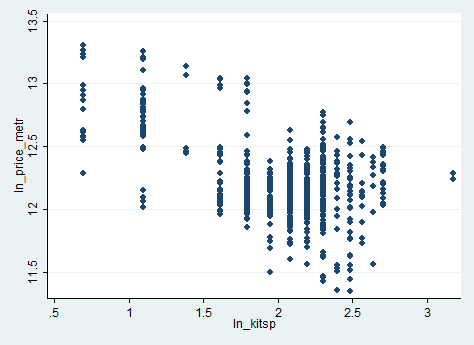
\includegraphics{kitsp.png}

\begin{verbatim}
scatter ln_price_metr ln_livesp
\end{verbatim}

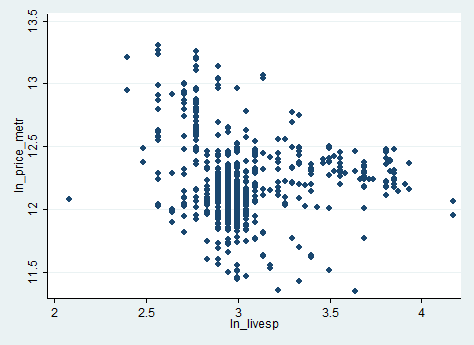
\includegraphics{livesp.png}

\begin{verbatim}
scatter ln_price_metr ln_dist
\end{verbatim}

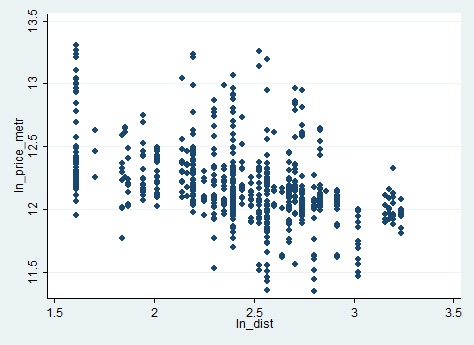
\includegraphics{dist.png}

\begin{verbatim}
scatter ln_price_metr ln_metrdist
\end{verbatim}

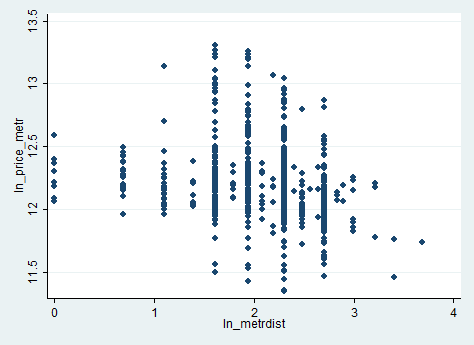
\includegraphics{metrdist.png}

Подозрительны переменные \texttt{ln\_kitsp} и \texttt{ln\_metrdist}
Проверим наличие гетероскедастичности с помощью тестов.

Тест Уайта строится по короткой команде:

\begin{verbatim}
estat imtest, white
\end{verbatim}

\begin{verbatim}
 file data/flats.dta not found
r(601);


last estimates not found
r(301);

end of do-file
r(301);
\end{verbatim}

Тест Уайта выявил гетероскедастичность. Что скажет тест Бройша-Пагана?

\begin{verbatim}
estat hettest, rhs mtest
\end{verbatim}

\begin{verbatim}
 file data/flats.dta not found
r(601);


last estimates not found
r(301);

end of do-file
r(301);
\end{verbatim}

И этот тест указывает на наличие нежелательной гетероскедастичности, особенно подозрительны переменные \texttt{ln\_kitsp} и \texttt{ln\_metrdist}.

Попробуем проверить ещё и через тест Голдфелда - Квандта. Сделаем его ручками.

Отсортируем наблюдения по возрастанию переменной \texttt{ln\_kitsp}, построим регрессию и сохраним остатки.

\begin{verbatim}
sort ln_kitsp
reg ln_price_metr ln_livesp ln_kitsp ln_dist ln_metrdist in 1 / 258
scalar rss1 = e(rss)
\end{verbatim}

\begin{verbatim}
 file data/flats.dta not found
r(601);


no variables defined
r(111);

end of do-file
r(111);
\end{verbatim}

Сохраним остатки и в последней части регрессии.

\begin{verbatim}
sort ln_kitsp
reg ln_price_metr ln_livesp ln_kitsp ln_dist ln_metrdist in 516 / 773
scalar rss2 = e(rss)
\end{verbatim}

\begin{verbatim}
 file data/flats.dta not found
r(601);


no variables defined
r(111);

end of do-file
r(111);
\end{verbatim}

Посчитаем тестовую F-статистику.

\begin{verbatim}
scalar F = rss2 / rss1
display F
display invFtail(258, 258, 0.05)
\end{verbatim}

\begin{verbatim}
 file data/flats.dta not found
r(601);


rss2 not found
r(111);

end of do-file
r(111);
\end{verbatim}

Тестовая статистика больше табличной, следовательно, гетероскедастичность присутствует.

Сейчас немного о способах борьбы с гетероскедастичностью. Подправим все коэффициенты исходной регрессии на гетероскедастичную переменную, например, на \texttt{ln\_kitsp}.

\begin{verbatim}
gen ln_price_metr_new = ln_price_metr / ln_kitsp
gen ln_livesp_new = ln_livesp / ln_kitsp
gen const_new = 1 / ln_kitsp
gen ln_dist_new = ln_dist / ln_kitsp
gen ln_metrdist_new = ln_metrdist / ln_kitsp
\end{verbatim}

\begin{verbatim}
 file data/flats.dta not found
r(601);


ln_price_metr not found
r(111);

end of do-file
r(111);
\end{verbatim}

И оценим регрессию с новыми переменными.

\begin{verbatim}
reg ln_price_metr_new ln_livesp_new const_new ln_dist_new ln_metrdist_new
\end{verbatim}

\begin{verbatim}
 file data/flats.dta not found
r(601);


no variables defined
r(111);

end of do-file
r(111);
\end{verbatim}

И полученные оценки будут эффективными оценками коэффициентов исходной регрессии.

Также можно использовать метод взвешенного МНК (WLS). Взвесим на стандартное отклонение фактора \texttt{ln\_kitsp}.

\begin{verbatim}
vwls ln_price_metr ln_livesp ln_kitsp ln_dist ln_metrdist, sd(ln_kitsp)
\end{verbatim}

\begin{verbatim}
 file data/flats.dta not found
r(601);


variable ln_price_metr not found
r(111);

end of do-file
r(111);
\end{verbatim}

Способ \#2. Используем робастные оценки Уайта.

\begin{verbatim}
reg ln_price_metr ln_livesp ln_kitsp ln_dist ln_metrdist, robust
\end{verbatim}

\begin{verbatim}
 file data/flats.dta not found
r(601);


no variables defined
r(111);

end of do-file
r(111);
\end{verbatim}

Робастные оценки Уайта позволяют снизить последствия гетероскедастичности через уменьшение стандартных ошибок коэффициентов регрессии.

\hypertarget{pca}{%
\chapter{PCA}\label{pca}}

\hypertarget{dinpanel}{%
\chapter{Динамические панели}\label{dinpanel}}

\hypertarget{tobit_heckit}{%
\chapter{TOBIT, HECKIT}\label{tobit_heckit}}

\begin{Shaded}
\begin{Highlighting}[]
\KeywordTok{library}\NormalTok{(ggplot2)}
\KeywordTok{library}\NormalTok{(AER) }\CommentTok{#tobit}
\KeywordTok{library}\NormalTok{(sampleSelection) }\CommentTok{#heckit}
\end{Highlighting}
\end{Shaded}

\begin{verbatim}
Error in library(sampleSelection): there is no package called 'sampleSelection'
\end{verbatim}

\begin{Shaded}
\begin{Highlighting}[]
\KeywordTok{library}\NormalTok{(}\StringTok{'ltm'}\NormalTok{) }\CommentTok{#margins}
\end{Highlighting}
\end{Shaded}

\begin{verbatim}
Error in library("ltm"): there is no package called 'ltm'
\end{verbatim}

\begin{Shaded}
\begin{Highlighting}[]
\KeywordTok{library}\NormalTok{(}\StringTok{'foreign'}\NormalTok{)}
\KeywordTok{library}\NormalTok{(skimr)}
\end{Highlighting}
\end{Shaded}

Данная глава посвящена моделям с цензурированными выборками. В таких выборках часть значений целевой переменной будет дискретной переменной, а часть - непрерывной. Простой пример, который указывается в некоторых учебниках, это исследование расходов семей на автомобили. Каждая семья может либо потратить какую-то сумму на автомобиль, либо, если она не может позволить себе автомобиль, то значение расходов будет равно нулю. Соответственно, переменная демонстрирует либо факт неучастия в покупке автомобиля, либо степень участия в виде суммы. Оценивается в данном случае обычная регрессионная модель, но с функцией правдоподобия следующего вида:

\begin{equation}
L=\prod_{y_{t}=0}\left(1-\Phi\left(\frac{\boldsymbol{x}_{t}^{\prime} \boldsymbol{\beta}}{\sigma}\right)\right) \prod_{y_{t}>0} \frac{1}{\sqrt{2 \pi} \sigma} \exp \left(-\frac{1}{2 \sigma^{2}}\left(y_{t}-\boldsymbol{x}_{t}^{\prime} \boldsymbol{\beta}\right)^{2}\right)
\end{equation}

Для начала подгрузим данные и визуализируем их. Этот датасет результаты тестирования двухсот школьников по шкале от 200 до 800 (apt), а также их успеваемость по чтению и математике (read и math соответственно). Построим гистограмму, наложив поверх неё функцию плотности нормального распределения.

\begin{Shaded}
\begin{Highlighting}[]
\NormalTok{data =}\StringTok{ }\KeywordTok{read.csv}\NormalTok{(}\StringTok{'tobit.csv'}\NormalTok{)}
\end{Highlighting}
\end{Shaded}

\begin{Shaded}
\begin{Highlighting}[]
\CommentTok{# Функция, генерирующая функцию плотности нормального распределения в соответствии с распределением вектора входных данных}
\NormalTok{f <-}\StringTok{ }\ControlFlowTok{function}\NormalTok{(x, var, }\DataTypeTok{bw =} \DecValTok{15}\NormalTok{) \{}
  \KeywordTok{dnorm}\NormalTok{(x, }\DataTypeTok{mean =} \KeywordTok{mean}\NormalTok{(var), }\KeywordTok{sd}\NormalTok{(var)) }\OperatorTok{*}\StringTok{ }\KeywordTok{length}\NormalTok{(var)  }\OperatorTok{*}\StringTok{ }\NormalTok{bw}
\NormalTok{\}}


\NormalTok{p <-}\StringTok{ }\KeywordTok{ggplot}\NormalTok{(data, }\KeywordTok{aes}\NormalTok{(}\DataTypeTok{x =}\NormalTok{ apt, }\DataTypeTok{fill=}\NormalTok{prog))}
\NormalTok{p }\OperatorTok{+}\StringTok{ }\KeywordTok{stat_bin}\NormalTok{(}\DataTypeTok{binwidth=}\DecValTok{15}\NormalTok{) }\OperatorTok{+}
\StringTok{  }\KeywordTok{stat_function}\NormalTok{(}\DataTypeTok{fun =}\NormalTok{ f, }\DataTypeTok{size =} \DecValTok{1}\NormalTok{,}
    \DataTypeTok{args =} \KeywordTok{list}\NormalTok{(}\DataTypeTok{var =}\NormalTok{ data}\OperatorTok{$}\NormalTok{apt))}
\end{Highlighting}
\end{Shaded}

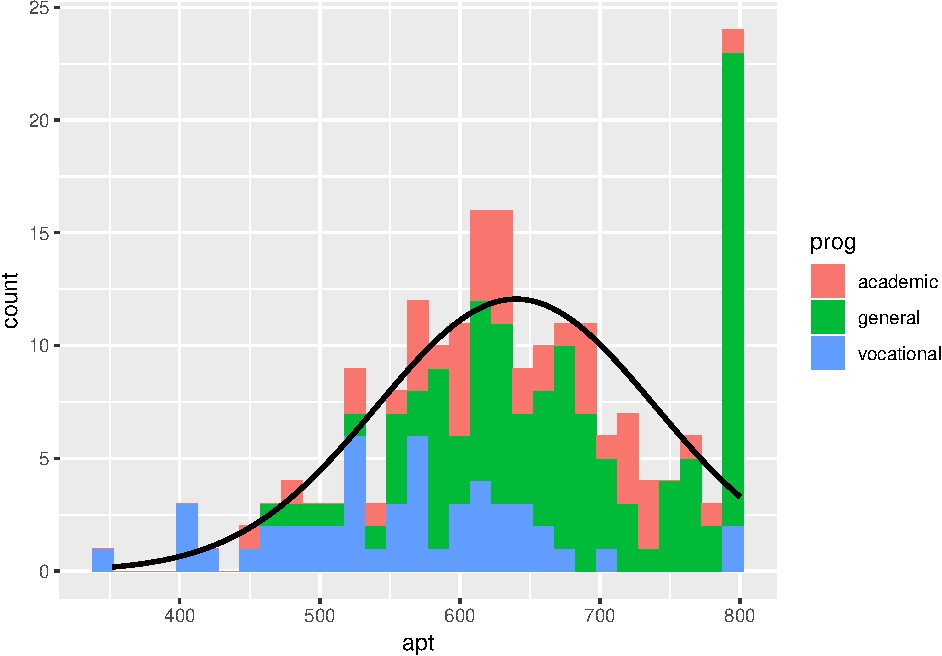
\includegraphics{13-tobit_heckit_files/figure-latex/hist plot chunk-1.pdf}

Как можем видеть, нашлось довольно много школьников, которые написали тест на высший балл. В связи с этим распределение даллеко от нормального из-за ограничений баллов теста. Вид выборки также довольно специфичен при взгляде на диаграмму рассеяния. Довольно различимая линейная зависимость как бы сплюснута сверху.

\begin{Shaded}
\begin{Highlighting}[]
\NormalTok{g <-}\StringTok{ }\KeywordTok{ggplot}\NormalTok{(data, }\KeywordTok{aes}\NormalTok{(math, apt, }\DataTypeTok{col =}\NormalTok{ prog))}
\NormalTok{g }\OperatorTok{+}\KeywordTok{geom_point}\NormalTok{()}
\end{Highlighting}
\end{Shaded}

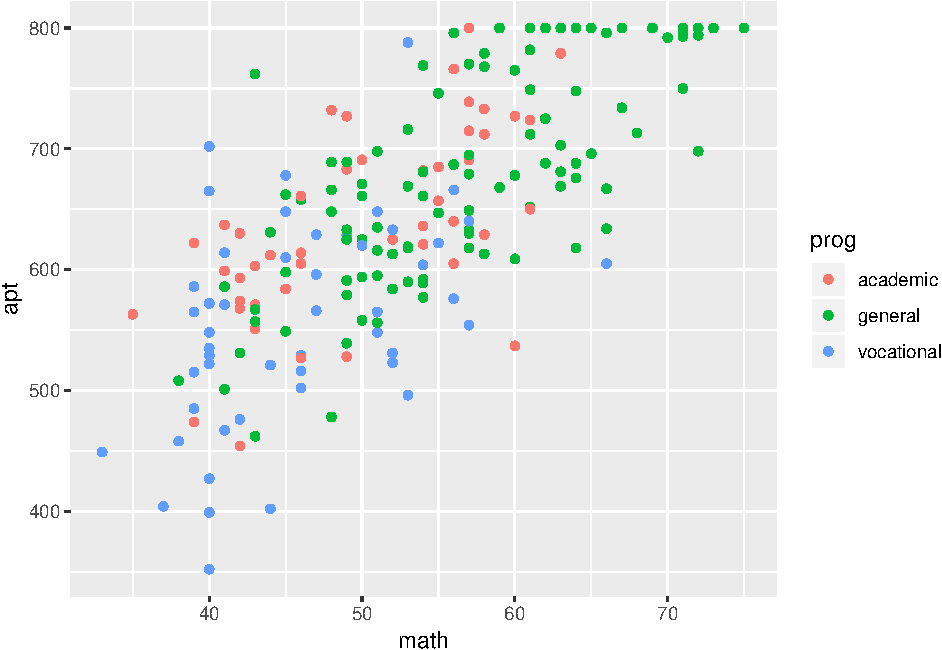
\includegraphics{13-tobit_heckit_files/figure-latex/scatter plot chunk-1.pdf}

Оценим Тобит-модель:

\begin{Shaded}
\begin{Highlighting}[]
\NormalTok{model_tobit =}\StringTok{ }\KeywordTok{tobit}\NormalTok{(apt }\OperatorTok{~}\StringTok{ }\NormalTok{math }\OperatorTok{+}\StringTok{ }\NormalTok{read, }\DataTypeTok{data =}\NormalTok{ data, }\DataTypeTok{right =} \DecValTok{800}\NormalTok{)}
\KeywordTok{summary}\NormalTok{(model_tobit)}
\end{Highlighting}
\end{Shaded}

\begin{verbatim}

Call:
tobit(formula = apt ~ math + read, right = 800, data = data)

Observations:
         Total  Left-censored     Uncensored Right-censored 
           200              0            183             17 

Coefficients:
             Estimate Std. Error z value Pr(>|z|)    
(Intercept) 159.00366   29.90374   5.317 1.05e-07 ***
math          6.34441    0.70306   9.024  < 2e-16 ***
read          2.88961    0.63295   4.565 4.99e-06 ***
Log(scale)    4.21923    0.05293  79.719  < 2e-16 ***
---
Signif. codes:  0 '***' 0.001 '**' 0.01 '*' 0.05 '.' 0.1 ' ' 1

Scale: 67.98 

Gaussian distribution
Number of Newton-Raphson Iterations: 5 
Log-likelihood: -1047 on 4 Df
Wald-statistic: 266.2 on 2 Df, p-value: < 2.22e-16 
\end{verbatim}

Модель Тобина имеет ряд ограничений. Основное из них -- это зависимость вероятности участия и интенсивности участия определяется одним и тем же набором переменных. Для преодоления этих ограничений была предложена модель Хекмана. В ней принятие решения ``участвовать - не участвовать'' и определение степени участия могут зависеть от разных переменных.

Загрузим другие данные во славу разнообразия.

\begin{Shaded}
\begin{Highlighting}[]
\NormalTok{data =}\StringTok{ }\KeywordTok{read.dta}\NormalTok{(}\StringTok{'data_alcohol&tobacco.dta'}\NormalTok{)}
\KeywordTok{summary}\NormalTok{(data)}
\end{Highlighting}
\end{Shaded}

\begin{verbatim}
     obs                 age           bluecol            lnx       
 Length:2724        Min.   :0.000   Min.   :0.0000   Min.   :11.76  
 Class :character   1st Qu.:1.000   1st Qu.:0.0000   1st Qu.:13.41  
 Mode  :character   Median :2.000   Median :0.0000   Median :13.76  
                    Mean   :2.408   Mean   :0.1468   Mean   :13.73  
                    3rd Qu.:4.000   3rd Qu.:0.0000   3rd Qu.:14.06  
                    Max.   :4.000   Max.   :1.0000   Max.   :15.33  
    flanders         nadults        ninfants           nkids       
 Min.   :0.0000   Min.   :1.00   Min.   :0.00000   Min.   :0.0000  
 1st Qu.:0.0000   1st Qu.:1.00   1st Qu.:0.00000   1st Qu.:0.0000  
 Median :0.0000   Median :2.00   Median :0.00000   Median :0.0000  
 Mean   :0.4519   Mean   :1.97   Mean   :0.04479   Mean   :0.5646  
 3rd Qu.:1.0000   3rd Qu.:2.00   3rd Qu.:0.00000   3rd Qu.:1.0000  
 Max.   :1.0000   Max.   :7.00   Max.   :2.00000   Max.   :5.0000  
     resid                shalc              shtob        
 Min.   :-0.9797682   Min.   :0.000000   Min.   :0.00000  
 1st Qu.: 0.0626030   1st Qu.:0.002906   1st Qu.:0.00000  
 Median : 0.1223031   Median :0.010898   Median :0.00000  
 Mean   : 0.0001171   Mean   :0.017828   Mean   :0.01224  
 3rd Qu.: 0.1854353   3rd Qu.:0.024244   3rd Qu.:0.01381  
 Max.   : 0.5795787   Max.   :0.211124   Max.   :0.19276  
    walloon          whitecol      shalc_tobit             alc        
 Min.   :0.0000   Min.   :0.000   Min.   :-0.005627   Min.   :0.0000  
 1st Qu.:0.0000   1st Qu.:0.000   1st Qu.: 0.010925   1st Qu.:1.0000  
 Median :0.0000   Median :0.000   Median : 0.015169   Median :1.0000  
 Mean   :0.3814   Mean   :0.333   Mean   : 0.015198   Mean   :0.8289  
 3rd Qu.:1.0000   3rd Qu.:1.000   3rd Qu.: 0.019735   3rd Qu.:1.0000  
 Max.   :1.0000   Max.   :1.000   Max.   : 0.032814   Max.   :1.0000  
      tob        
 Min.   :0.0000  
 1st Qu.:0.0000  
 Median :0.0000  
 Mean   :0.3803  
 3rd Qu.:1.0000  
 Max.   :1.0000  
\end{verbatim}

\begin{Shaded}
\begin{Highlighting}[]
\NormalTok{f <-}\StringTok{ }\ControlFlowTok{function}\NormalTok{(x, var, }\DataTypeTok{bw =} \DecValTok{15}\NormalTok{) \{}
  \KeywordTok{dnorm}\NormalTok{(x, }\DataTypeTok{mean =} \KeywordTok{mean}\NormalTok{(var), }\KeywordTok{sd}\NormalTok{(var)) }\OperatorTok{*}\StringTok{ }\KeywordTok{length}\NormalTok{(var)  }\OperatorTok{*}\StringTok{ }\NormalTok{bw}
\NormalTok{\}}


\NormalTok{p <-}\StringTok{ }\KeywordTok{ggplot}\NormalTok{(data, }\KeywordTok{aes}\NormalTok{(}\DataTypeTok{x =}\NormalTok{ shalc))}
\NormalTok{p }\OperatorTok{+}\StringTok{ }\KeywordTok{stat_bin}\NormalTok{(}\DataTypeTok{binwidth=}\FloatTok{0.01}\NormalTok{) }\OperatorTok{+}
\StringTok{  }\KeywordTok{stat_function}\NormalTok{(}\DataTypeTok{fun =}\NormalTok{ f, }\DataTypeTok{size =} \DecValTok{1}\NormalTok{,}
    \DataTypeTok{args =} \KeywordTok{list}\NormalTok{(}\DataTypeTok{var =}\NormalTok{ data}\OperatorTok{$}\NormalTok{alc))}
\end{Highlighting}
\end{Shaded}

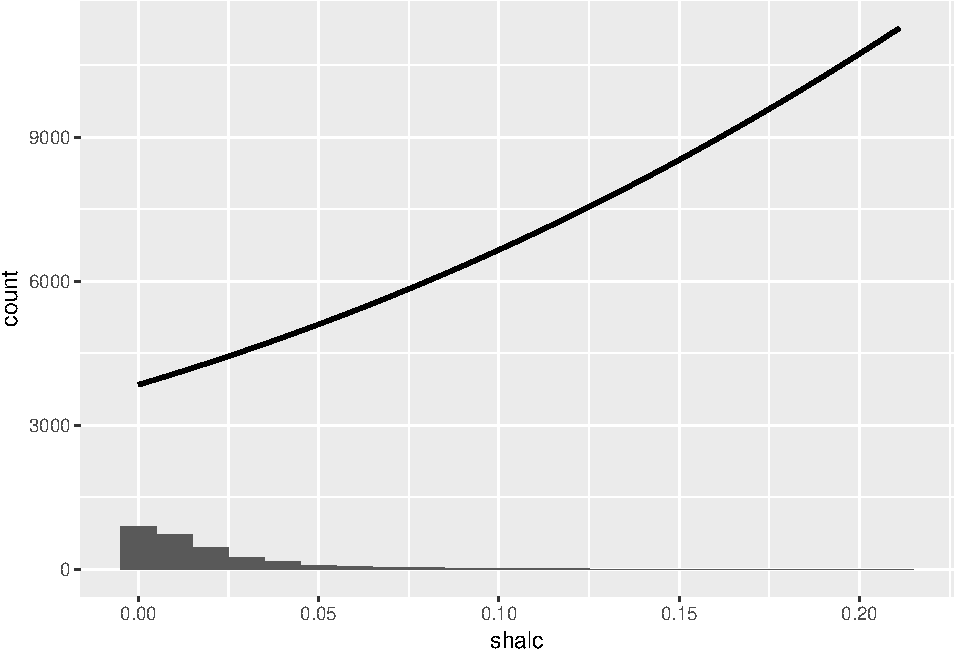
\includegraphics{13-tobit_heckit_files/figure-latex/unnamed-chunk-2-1.pdf}

\begin{Shaded}
\begin{Highlighting}[]
\NormalTok{heck1 =}\StringTok{ }\KeywordTok{heckit}\NormalTok{(alc }\OperatorTok{~}\StringTok{ }\NormalTok{age }\OperatorTok{+}\StringTok{ }\NormalTok{nadults }\OperatorTok{+}\StringTok{ }\NormalTok{nkids }\OperatorTok{+}\StringTok{ }\NormalTok{lnx }\OperatorTok{+}\StringTok{ }\NormalTok{walloon, shalc }\OperatorTok{~}\StringTok{  }\NormalTok{age }\OperatorTok{+}\StringTok{ }\NormalTok{nadults }\OperatorTok{+}\StringTok{ }\NormalTok{nkids }\OperatorTok{+}\StringTok{ }\NormalTok{lnx }\OperatorTok{+}\StringTok{ }\NormalTok{walloon, }\DataTypeTok{data =}\NormalTok{ data, }\DataTypeTok{method =} \StringTok{'ml'}\NormalTok{)}
\end{Highlighting}
\end{Shaded}

\begin{verbatim}
Error in heckit(alc ~ age + nadults + nkids + lnx + walloon, shalc ~ age + : could not find function "heckit"
\end{verbatim}

\begin{Shaded}
\begin{Highlighting}[]
\KeywordTok{summary}\NormalTok{(heck1)}
\end{Highlighting}
\end{Shaded}

\begin{verbatim}
Error in summary(heck1): object 'heck1' not found
\end{verbatim}

\begin{Shaded}
\begin{Highlighting}[]
\NormalTok{heck2 =}\StringTok{ }\KeywordTok{heckit2fit}\NormalTok{(alc }\OperatorTok{~}\StringTok{ }\NormalTok{age }\OperatorTok{+}\StringTok{ }\NormalTok{nadults }\OperatorTok{+}\StringTok{ }\NormalTok{nkids }\OperatorTok{+}\StringTok{ }\NormalTok{lnx }\OperatorTok{+}\StringTok{ }\NormalTok{walloon, shalc }\OperatorTok{~}\StringTok{  }\NormalTok{age }\OperatorTok{+}\StringTok{ }\NormalTok{nadults }\OperatorTok{+}\StringTok{ }\NormalTok{nkids }\OperatorTok{+}\StringTok{ }\NormalTok{lnx }\OperatorTok{+}\StringTok{ }\NormalTok{walloon, }\DataTypeTok{data =}\NormalTok{ data)}
\end{Highlighting}
\end{Shaded}

\begin{verbatim}
Error in heckit2fit(alc ~ age + nadults + nkids + lnx + walloon, shalc ~ : could not find function "heckit2fit"
\end{verbatim}

\begin{Shaded}
\begin{Highlighting}[]
\KeywordTok{summary}\NormalTok{(heck2)}
\end{Highlighting}
\end{Shaded}

\begin{verbatim}
Error in summary(heck2): object 'heck2' not found
\end{verbatim}

Теперь то же самое в STATA.

\begin{verbatim}
clear
use tobit
summarize
\end{verbatim}

\begin{verbatim}
    Variable |        Obs        Mean    Std. Dev.       Min        Max
-------------+---------------------------------------------------------
          v1 |        200        99.5    57.87918          0        199
    unnamed0 |        200        99.5    57.87918          0        199
          id |        200       100.5    57.87918          1        200
        read |        200       52.23    10.25294         28         76
        math |        200      52.645    9.368448         33         75
-------------+---------------------------------------------------------
        prog |          0
         apt |        200     640.035    99.21903        352        800
         top |        200        .915    .2795815          0          1
\end{verbatim}

\begin{verbatim}
egen prog_2 = group(prog)
tobit apt read math i.prog_2, ul
\end{verbatim}

\begin{verbatim}
Tobit regression                                Number of obs     =        200
                                                LR chi2(4)        =     188.97
                                                Prob > chi2       =     0.0000
Log likelihood = -1041.0629                     Pseudo R2         =     0.0832

------------------------------------------------------------------------------
         apt |      Coef.   Std. Err.      t    P>|t|     [95% Conf. Interval]
-------------+----------------------------------------------------------------
        read |   2.697939    .618798     4.36   0.000     1.477582    3.918296
        math |   5.914485   .7098063     8.33   0.000     4.514647    7.314323
             |
      prog_2 |
          2  |  -12.71476   12.40629    -1.02   0.307    -37.18173     11.7522
          3  |   -46.1439   13.72401    -3.36   0.001     -73.2096   -19.07821
             |
       _cons |    209.566   32.77154     6.39   0.000     144.9359    274.1961
-------------+----------------------------------------------------------------
      /sigma |   65.67672   3.481272                      58.81116    72.54228
------------------------------------------------------------------------------
             0  left-censored observations
           183     uncensored observations
            17 right-censored observations at apt >= 800
\end{verbatim}

\begin{verbatim}
clear all
use data_alcohol&tobacco
heckman shalc age nadults nkids lnx walloon, select(alc = age nadults nkids lnx walloon)
\end{verbatim}

\begin{verbatim}
Iteration 0:   log likelihood =  4309.5307  
Iteration 1:   log likelihood =  4311.3949  
Iteration 2:   log likelihood =  4311.4638  
Iteration 3:   log likelihood =  4311.4649  
Iteration 4:   log likelihood =  4311.4649  

Heckman selection model                         Number of obs     =      2,724
(regression model with sample selection)        Censored obs      =        466
                                                Uncensored obs    =      2,258

                                                Wald chi2(5)      =     126.74
Log likelihood =  4311.465                      Prob > chi2       =     0.0000

------------------------------------------------------------------------------
             |      Coef.   Std. Err.      z    P>|z|     [95% Conf. Interval]
-------------+----------------------------------------------------------------
shalc        |
         age |   .0022075   .0003854     5.73   0.000     .0014521     .002963
     nadults |  -.0017463   .0006455    -2.71   0.007    -.0030114   -.0004812
       nkids |  -.0021381    .000564    -3.79   0.000    -.0032435   -.0010327
         lnx |   -.001557   .0014823    -1.05   0.294    -.0044622    .0013483
     walloon |   .0025647   .0009575     2.68   0.007     .0006881    .0044413
       _cons |   .0413301   .0205898     2.01   0.045     .0009749    .0816853
-------------+----------------------------------------------------------------
alc          |
         age |    .064492   .0233269     2.76   0.006     .0187722    .1102118
     nadults |  -.0865676   .0419754    -2.06   0.039    -.1688379   -.0042973
       nkids |  -.0847672   .0362055    -2.34   0.019    -.1557287   -.0138058
         lnx |   .8839885   .0758532    11.65   0.000      .735319    1.032658
     walloon |   .1975137    .062286     3.17   0.002     .0754353    .3195921
       _cons |  -11.12847   .9982321   -11.15   0.000    -13.08497   -9.171975
-------------+----------------------------------------------------------------
     /athrho |  -.0062433   .1345632    -0.05   0.963    -.2699823    .2574956
    /lnsigma |  -3.841538   .0148838  -258.10   0.000    -3.870709   -3.812366
-------------+----------------------------------------------------------------
         rho |  -.0062433   .1345579                     -.2636083    .2519516
       sigma |   .0214606   .0003194                      .0208436    .0220958
      lambda |   -.000134   .0028877                     -.0057938    .0055259
------------------------------------------------------------------------------
LR test of indep. eqns. (rho = 0):   chi2(1) =     0.00   Prob > chi2 = 0.9640
\end{verbatim}

\begin{verbatim}
heckman shalc age nadults nkids lnx walloon, select(alc = age nadults nkids lnx walloon) twostep
\end{verbatim}

\begin{verbatim}
> nx walloon) twostep

Heckman selection model -- two-step estimates   Number of obs     =      2,724
(regression model with sample selection)        Censored obs      =        466
                                                Uncensored obs    =      2,258

                                                Wald chi2(5)      =     125.15
                                                Prob > chi2       =     0.0000

------------------------------------------------------------------------------
             |      Coef.   Std. Err.      z    P>|z|     [95% Conf. Interval]
-------------+----------------------------------------------------------------
shalc        |
         age |    .002117   .0005482     3.86   0.000     .0010426    .0031915
     nadults |  -.0016402    .000792    -2.07   0.038    -.0031925   -.0000879
       nkids |  -.0020387   .0007089    -2.88   0.004    -.0034282   -.0006492
         lnx |  -.0027209   .0052148    -0.52   0.602    -.0129417    .0074998
     walloon |   .0023175   .0014319     1.62   0.106    -.0004889     .005124
       _cons |   .0584579   .0763935     0.77   0.444    -.0912706    .2081865
-------------+----------------------------------------------------------------
alc          |
         age |    .064482   .0233247     2.76   0.006     .0187665    .1101975
     nadults |  -.0865298   .0419629    -2.06   0.039    -.1687756   -.0042839
       nkids |  -.0847535   .0362048    -2.34   0.019    -.1557135   -.0137934
         lnx |   .8839584   .0758491    11.65   0.000     .7352969     1.03262
     walloon |   .1974812   .0622813     3.17   0.002     .0754121    .3195503
       _cons |   -11.1281   .9981866   -11.15   0.000    -13.08451   -9.171695
-------------+----------------------------------------------------------------
mills        |
      lambda |   -.003805    .016022    -0.24   0.812    -.0352075    .0275975
-------------+----------------------------------------------------------------
         rho |   -0.17633
       sigma |  .02157888
------------------------------------------------------------------------------
\end{verbatim}

\hypertarget{treatment}{%
\chapter{Treatment effect}\label{treatment}}

\hypertarget{compatability}{%
\chapter{Что-то там про совместимость и языки}\label{compatability}}

\hypertarget{dict}{%
\chapter{Словарь}\label{dict}}

\bibliography{book.bib,packages.bib}


\end{document}
